% Options for packages loaded elsewhere
\PassOptionsToPackage{unicode}{hyperref}
\PassOptionsToPackage{hyphens}{url}
%
\documentclass[
]{book}
\usepackage{lmodern}
\usepackage{amssymb,amsmath}
\usepackage{ifxetex,ifluatex}
\ifnum 0\ifxetex 1\fi\ifluatex 1\fi=0 % if pdftex
  \usepackage[T1]{fontenc}
  \usepackage[utf8]{inputenc}
  \usepackage{textcomp} % provide euro and other symbols
\else % if luatex or xetex
  \usepackage{unicode-math}
  \defaultfontfeatures{Scale=MatchLowercase}
  \defaultfontfeatures[\rmfamily]{Ligatures=TeX,Scale=1}
\fi
% Use upquote if available, for straight quotes in verbatim environments
\IfFileExists{upquote.sty}{\usepackage{upquote}}{}
\IfFileExists{microtype.sty}{% use microtype if available
  \usepackage[]{microtype}
  \UseMicrotypeSet[protrusion]{basicmath} % disable protrusion for tt fonts
}{}
\makeatletter
\@ifundefined{KOMAClassName}{% if non-KOMA class
  \IfFileExists{parskip.sty}{%
    \usepackage{parskip}
  }{% else
    \setlength{\parindent}{0pt}
    \setlength{\parskip}{6pt plus 2pt minus 1pt}}
}{% if KOMA class
  \KOMAoptions{parskip=half}}
\makeatother
\usepackage{xcolor}
\IfFileExists{xurl.sty}{\usepackage{xurl}}{} % add URL line breaks if available
\IfFileExists{bookmark.sty}{\usepackage{bookmark}}{\usepackage{hyperref}}
\hypersetup{
  pdftitle={Guide d'utilisation},
  pdfauthor={Corentin J Gosling},
  hidelinks,
  pdfcreator={LaTeX via pandoc}}
\urlstyle{same} % disable monospaced font for URLs
\usepackage{color}
\usepackage{fancyvrb}
\newcommand{\VerbBar}{|}
\newcommand{\VERB}{\Verb[commandchars=\\\{\}]}
\DefineVerbatimEnvironment{Highlighting}{Verbatim}{commandchars=\\\{\}}
% Add ',fontsize=\small' for more characters per line
\usepackage{framed}
\definecolor{shadecolor}{RGB}{248,248,248}
\newenvironment{Shaded}{\begin{snugshade}}{\end{snugshade}}
\newcommand{\AlertTok}[1]{\textcolor[rgb]{0.94,0.16,0.16}{#1}}
\newcommand{\AnnotationTok}[1]{\textcolor[rgb]{0.56,0.35,0.01}{\textbf{\textit{#1}}}}
\newcommand{\AttributeTok}[1]{\textcolor[rgb]{0.77,0.63,0.00}{#1}}
\newcommand{\BaseNTok}[1]{\textcolor[rgb]{0.00,0.00,0.81}{#1}}
\newcommand{\BuiltInTok}[1]{#1}
\newcommand{\CharTok}[1]{\textcolor[rgb]{0.31,0.60,0.02}{#1}}
\newcommand{\CommentTok}[1]{\textcolor[rgb]{0.56,0.35,0.01}{\textit{#1}}}
\newcommand{\CommentVarTok}[1]{\textcolor[rgb]{0.56,0.35,0.01}{\textbf{\textit{#1}}}}
\newcommand{\ConstantTok}[1]{\textcolor[rgb]{0.00,0.00,0.00}{#1}}
\newcommand{\ControlFlowTok}[1]{\textcolor[rgb]{0.13,0.29,0.53}{\textbf{#1}}}
\newcommand{\DataTypeTok}[1]{\textcolor[rgb]{0.13,0.29,0.53}{#1}}
\newcommand{\DecValTok}[1]{\textcolor[rgb]{0.00,0.00,0.81}{#1}}
\newcommand{\DocumentationTok}[1]{\textcolor[rgb]{0.56,0.35,0.01}{\textbf{\textit{#1}}}}
\newcommand{\ErrorTok}[1]{\textcolor[rgb]{0.64,0.00,0.00}{\textbf{#1}}}
\newcommand{\ExtensionTok}[1]{#1}
\newcommand{\FloatTok}[1]{\textcolor[rgb]{0.00,0.00,0.81}{#1}}
\newcommand{\FunctionTok}[1]{\textcolor[rgb]{0.00,0.00,0.00}{#1}}
\newcommand{\ImportTok}[1]{#1}
\newcommand{\InformationTok}[1]{\textcolor[rgb]{0.56,0.35,0.01}{\textbf{\textit{#1}}}}
\newcommand{\KeywordTok}[1]{\textcolor[rgb]{0.13,0.29,0.53}{\textbf{#1}}}
\newcommand{\NormalTok}[1]{#1}
\newcommand{\OperatorTok}[1]{\textcolor[rgb]{0.81,0.36,0.00}{\textbf{#1}}}
\newcommand{\OtherTok}[1]{\textcolor[rgb]{0.56,0.35,0.01}{#1}}
\newcommand{\PreprocessorTok}[1]{\textcolor[rgb]{0.56,0.35,0.01}{\textit{#1}}}
\newcommand{\RegionMarkerTok}[1]{#1}
\newcommand{\SpecialCharTok}[1]{\textcolor[rgb]{0.00,0.00,0.00}{#1}}
\newcommand{\SpecialStringTok}[1]{\textcolor[rgb]{0.31,0.60,0.02}{#1}}
\newcommand{\StringTok}[1]{\textcolor[rgb]{0.31,0.60,0.02}{#1}}
\newcommand{\VariableTok}[1]{\textcolor[rgb]{0.00,0.00,0.00}{#1}}
\newcommand{\VerbatimStringTok}[1]{\textcolor[rgb]{0.31,0.60,0.02}{#1}}
\newcommand{\WarningTok}[1]{\textcolor[rgb]{0.56,0.35,0.01}{\textbf{\textit{#1}}}}
\usepackage{longtable,booktabs}
% Correct order of tables after \paragraph or \subparagraph
\usepackage{etoolbox}
\makeatletter
\patchcmd\longtable{\par}{\if@noskipsec\mbox{}\fi\par}{}{}
\makeatother
% Allow footnotes in longtable head/foot
\IfFileExists{footnotehyper.sty}{\usepackage{footnotehyper}}{\usepackage{footnote}}
\makesavenoteenv{longtable}
\usepackage{graphicx,grffile}
\makeatletter
\def\maxwidth{\ifdim\Gin@nat@width>\linewidth\linewidth\else\Gin@nat@width\fi}
\def\maxheight{\ifdim\Gin@nat@height>\textheight\textheight\else\Gin@nat@height\fi}
\makeatother
% Scale images if necessary, so that they will not overflow the page
% margins by default, and it is still possible to overwrite the defaults
% using explicit options in \includegraphics[width, height, ...]{}
\setkeys{Gin}{width=\maxwidth,height=\maxheight,keepaspectratio}
% Set default figure placement to htbp
\makeatletter
\def\fps@figure{htbp}
\makeatother
\setlength{\emergencystretch}{3em} % prevent overfull lines
\providecommand{\tightlist}{%
  \setlength{\itemsep}{0pt}\setlength{\parskip}{0pt}}
\setcounter{secnumdepth}{5}
\usepackage{booktabs}
\usepackage[]{natbib}
\bibliographystyle{apalike}

\title{Guide d'utilisation}
\author{Corentin J Gosling}
\date{2020-10-25}

\begin{document}
\maketitle

{
\setcounter{tocdepth}{2}
\tableofcontents
}
\hypertarget{intro}{%
\chapter{Introduction}\label{intro}}

\begin{itemize}
\item
  \textbf{ATTENTION}
  Ce manuel n'a pas fait l'objet d'une évaluation indépendante par les pairs : il reste encore un document de travail. Des corrections/améliorations seront donc apportées dans les prochaines actualisations du manuel.
\item
  \textbf{Quel est le but de ce manuel} ?
  L'unique objectif de ce manuel est de fournir un support technique pour analyser des données \textbf{indépendantes} à l'aide du logiciel R.
\item
  \textbf{Que sont des données indépendantes}
  Des données indépendantes correspondent à des plans expérimentaux où chacune de vos observations collectées sont indépendantes les unes des autres. Par exemple, si vos unités statistiques sont des individus, les données seront dites indépendantes si les informations collectées auprès d'un individu sont indépendantes des informations collectées auprès des autres individus de l'échantillon.

  \begin{itemize}
  \item
    En psychologie cognitive, des études classiques produisant des données non-indépendantes sont les études demandant à des participants de compléter des tâches expérimentales comportant de multiples essais. Dans cette situation, votre unité statistique de plus bas niveau (l'essai) n'est pas indépendante. La performance à un essai donné aura plus de chance d'être corrélée à la performance aux autres essais du même individu qu'à la performance aux essais réalisés par d'autres individus.
  \item
    En neuropsychologie, des études classiques produisant des données non-indépendantes sont les études collectant des données de patients provenant de divers hôpitaux. Dans cette situation, votre unité statistique de plus bas niveau (le patient) n'est pas indépendante. La performance d'un patient aura plus de chance d'être corrélée à la performance de patients du même hôpital qu'à la performance de patients provenant d'hôpitaux différents.
  \item
    En psychologie développementale, des études classiques produisant des données non-indépendantes sont les études collectant des données d'enfants répartis dans différentes classes ou écoles. Là encore, dans cette situation, votre unité statistique de plus bas niveau (l'enfant) n'est pas indépendante. La performance d'un enfant aura plus de chances d'être corrélée à la performance d'enfants de la même classe/école qu'à la performance d'enfants provenant de classes/écoles différentes.
  \end{itemize}
\end{itemize}

Dans ces situations de non-indépendance, deux solutions sont généralement utilisées.

\begin{enumerate}
\def\labelenumi{\arabic{enumi})}
\item
  La solution la plus recommandée est d'utiliser des analyses statistiques adaptées aux données dépendantes, parfois appelées analyses hiérarchiques ou multiniveaux (telles que les ANOVAs à mesures répétées, les modèles mixtes, les équations d'estimation généralisées, etc..). La façon d'implanter ces analyses dans R n'est pas décrite dans ce manuel, qui est centré sur les analyses adaptées aux données indépendantes. 
\item
  Une autre solution est d'aggréger vos unités statistiques de plus bas niveau non-indépendantes (e.g., les différents essais d'un même participant ou les différents enfants d'une même classe) au sein d'unités statistiques de plus haut niveau mais indépendantes. Dans une situation expérimentale comportant une tâche avec de nombreux essais, il est possible d'aggréger tous les essais en en faisant une moyenne pour chaque participant. Ce score aggrégé, propre à chaque participant, sera parfaitement indépendant du score aggrégé des autres participants. Il devient possible d'utiliser des analyses statistiques pour données indépendantes sur ce score aggrégé. Ici votre unité statistique de bas niveau (les essais) était non-indépendante, et l'utilisation d'une unité statistique de plus haut niveau (les participants) permet d'avoir des données indépendantes. Cependant, cette seconde approche n'est pas recommandée (voir par exemple la discussion au sujet des données non-indépendantes proposée par Aarts et al.~(2014) dans Nature Neuroscience).
\end{enumerate}

\begin{itemize}
\item
  \textbf{Pourquoi décrire ces analyses sur le logiciel R et non des logiciels standards (SPSS, Jamovi, \ldots{} ?)}
  Le logiciel R présente plusieurs avantages comparativements à certains logiciels statistiques plus fréquemment utilisés : (1) R est gratuit, (2) R permet de réaliser une très grande variété d'analyses statistiques et (3) R permet de partager aux lecteurs de vos articles le code qui accompagne l'analyse des données.
\item
  \textbf{Les analyses statistiques décrites dans ce manuel sont-elles suffisantes pour analyser des données collectées lors d'une étude ?}
  A l'heure actuelle, en plus des analyses statistiques, ce manuel décrit comment observer la distribution de vos variables, comment faire des graphiques illustrant les analyses statistiques réalisées et comment réaliser différents tests post-hoc et obtenir des tailles d'effet.
  En revanche, ce manuel suppose que les hypothèses fondamentales des différentes analyses statistiques sont respectées (e.g., si vous utilisez une régression linéaire, le code proposé dans ce manuel suppose que l'hypothèse de normalité des résidus est respectée).
\end{itemize}

\hypertarget{familiarisation-avec-r}{%
\chapter{Familiarisation avec R}\label{familiarisation-avec-r}}

\hypertarget{installation-de-r-et-r-studio}{%
\section{Installation de R et R studio}\label{installation-de-r-et-r-studio}}

Pour ce manuel, nous vous recommandons de travailler avec R Studio. R Studio est simplement un add-on de R permettant d'avoir une interface graphique afin -- entre autre -- de pouvoir visualiser facilement ses données.
L'installation de R Studio se fait en 2 temps. Tout d'abord, rendez vous sur la page de R puis installez la version basique de R (\url{https://cran.r-project.org/mirrors.html}). Si vous travaillez sous Mac OS X, rendez vous sur : \url{https://cran.r-project.org/bin/macosx/}.
Une fois que R est installé, vous allez pouvoir installer R Studio. Pour ce faire, rendez vous sur (\url{https://rstudio.com/products/rstudio/download/}).

\hypertarget{fonctionnement-des-packages}{%
\section{Fonctionnement des packages}\label{fonctionnement-des-packages}}

Dans R, un « package » correspond à une sorte de petit programme pouvant être ajouté à R et vous permettant d'accéder à des fonctionnalités non directement disponibles dans la version basique de R. Par exemple, la version de base de R dispose d'une fonction permettant de calculer une corrélation (cor.test) mais ne comporte pas de fonction permettant de faire des modèles mixtes. Un « package » nommé lme4 a été créé pour permettre de réaliser ces modèles mixtes dans R.
Chaque package ne nécessite d'être installé qu'une seule fois. Ceci est fait grâce à la commande :
install.packages(``Nom-du-package'')
En revanche, à chaque fois que R est fermé puis ouvert (ou juste après l'installation d'un package), vous devez obligatoirement charger la librairie d'un package si vous souhaitez l'utiliser. Ceci est fait grâce à la commande :
library(Nom-du-package)
En résumé, vous ne devez installer le package dont vous avez besoin qu'une seule fois. A chaque fois que vous fermez R, vous devrez recharger la librairie associée au package lors de la prochaine ouverture si vous souhaitez l'utiliser à nouveau.

\hypertarget{guillemets-et-r}{%
\section{Guillemets et R}\label{guillemets-et-r}}

Dans R, l'utilisation de guillemets est fréquente. Cependant, un point important est qu'il ne tolère qu'un seul type de guillemets : \texttt{"}
Tous les autres types de guillemets (e.g., \texttt{«} \texttt{»}) conduiront à un message d'erreur.
Si jamais vous importez un code R rédigé sur un éditeur de texte, il est important de convertir les guillements dans le bon format. A partir de word, vous pouvez créer ces guillemets en cliquant sur la touche de guillemet classique («) puis en appuyant immédiatement après sur les touches \texttt{ctrl+z}. Les guillemets américains requis par R (") s'afficheront automatiquement.

\hypertarget{six-commandes-indispensables}{%
\section{Six commandes INDISPENSABLES}\label{six-commandes-indispensables}}

\begin{enumerate}
\def\labelenumi{\arabic{enumi}.}
\tightlist
\item
  \texttt{\textless{}-} Assigne ce qui vient à droite de la flèche à ce qui est à gauche de la flèche. Par exemple, si un utilisateur tape la ligne de commande \texttt{x\textless{}-2} , alors la commande \texttt{x} affichera ce qui est contenu dans x (ici 2) et la commande \texttt{x+3} donnera le résultat 5. 
\end{enumerate}

\begin{Shaded}
\begin{Highlighting}[]
\NormalTok{x <-}\StringTok{ }\DecValTok{2}
\NormalTok{x}
\end{Highlighting}
\end{Shaded}

\begin{verbatim}
## [1] 2
\end{verbatim}

\begin{Shaded}
\begin{Highlighting}[]
\NormalTok{x }\OperatorTok{+}\StringTok{ }\DecValTok{3}
\end{Highlighting}
\end{Shaded}

\begin{verbatim}
## [1] 5
\end{verbatim}

\begin{enumerate}
\def\labelenumi{\arabic{enumi}.}
\setcounter{enumi}{1}
\item
  \texttt{summary()} Cette fonction permet de produire le résumé d'un jeu de données ou des résultats de divers modèles statistiques.
\item
  \texttt{\textasciitilde{}} Au sein d'une formule, ce qui vient à gauche du tilde correspond à la variable dépendante et ce qui vient à droite du tilde correspond à la variable indépendante. La commande \texttt{y\ \textasciitilde{}\ x} signifie que l'on souhaite savoir si \texttt{x} prédit, ou est lié, à \texttt{y}. 
\item
  \texttt{+} Au sein d'une formule, le symbole \texttt{+} sépare 2 effets principaux. Par exemple, la commande \texttt{y\ \textasciitilde{}\ x\ +\ z} signifie que l'on souhaite obtenir l'effet principal de \texttt{x} et l'effet principal de \texttt{z} sur la variable dépendante \texttt{y}.
\item
  \texttt{*} permet de créer des plans factoriels. Par exemple, la commande \texttt{y\ \textless{}-\ x\ *\ z} signifie que l'on souhaite obtenir l'effet principal de \texttt{x}, l'effet principal de \texttt{z} ainsi que l'interaction entre x et z.
\item
  \texttt{:} Au sein d'une formule, le symbole \texttt{:} permet de créer une interaction entre deux termes. Par exemple, la commande \texttt{y\ \textless{}-\ x\ :\ z} signifie que l'on souhaite obtenir l'interaction entre \texttt{x} et \texttt{z}. Les commandes \texttt{y\ \textless{}-\ x\ +\ z\ +\ x:z} et \texttt{y\ \textless{}-\ x\ *\ z} produisent des résultats identiques. 
\end{enumerate}

En résumé, pour construire un modèle statistique, R utilise les commandes suivantes

\begin{Shaded}
\begin{Highlighting}[]
\NormalTok{formula =}\StringTok{ }\NormalTok{y }\OperatorTok{~}\StringTok{ }\NormalTok{x }\CommentTok{# effet principal de x sur y }
\NormalTok{formula =}\StringTok{ }\NormalTok{y }\OperatorTok{~}\StringTok{ }\NormalTok{x }\OperatorTok{+}\StringTok{ }\NormalTok{z }\CommentTok{# effets principaux de x et z sur y }
\NormalTok{formula =}\StringTok{ }\NormalTok{y }\OperatorTok{~}\StringTok{ }\NormalTok{x }\OperatorTok{+}\StringTok{ }\NormalTok{z }\OperatorTok{+}\StringTok{ }\NormalTok{m }\CommentTok{# effets principaux de x, z et m sur y }
\NormalTok{formula =}\StringTok{ }\NormalTok{y }\OperatorTok{~}\StringTok{ }\NormalTok{x }\OperatorTok{+}\StringTok{ }\NormalTok{z }\OperatorTok{+}\StringTok{ }\NormalTok{m }\OperatorTok{+}\StringTok{ }\NormalTok{x}\OperatorTok{:}\NormalTok{z }\CommentTok{# effets principaux de x, z et m sur y et interaction entre x et z sur y}
\NormalTok{formula =}\StringTok{ }\NormalTok{y }\OperatorTok{~}\StringTok{ }\NormalTok{x}\OperatorTok{*}\NormalTok{z }\OperatorTok{+}\StringTok{ }\NormalTok{m }\CommentTok{# commande strictement équivalente à la ligne précédente}
\NormalTok{formula =}\StringTok{ }\NormalTok{y }\OperatorTok{~}\StringTok{ }\NormalTok{x }\OperatorTok{+}\StringTok{ }\NormalTok{z }\OperatorTok{+}\StringTok{ }\NormalTok{m }\OperatorTok{+}\StringTok{ }\NormalTok{x}\OperatorTok{:}\NormalTok{z }\OperatorTok{+}\StringTok{ }\NormalTok{x}\OperatorTok{:}\NormalTok{m }\OperatorTok{+}\StringTok{ }\NormalTok{m}\OperatorTok{:}\NormalTok{z }\OperatorTok{+}\StringTok{ }\NormalTok{x}\OperatorTok{:}\NormalTok{z}\OperatorTok{:}\NormalTok{m }\CommentTok{# analyse de tous les effets principaux, des 3 interactions simples et de l'interaction double sur y}
\NormalTok{formula =}\StringTok{ }\NormalTok{y }\OperatorTok{~}\StringTok{ }\NormalTok{x}\OperatorTok{*}\NormalTok{m}\OperatorTok{*}\NormalTok{z }\CommentTok{# commande strictement équivalente à la ligne précédente}
\end{Highlighting}
\end{Shaded}

\hypertarget{quelques-commandes-non-indispensables}{%
\section{Quelques commandes non-indispensables}\label{quelques-commandes-non-indispensables}}

\texttt{c()} Permet de créer un vecteur composé de nombres ou de caractères. Chaque élément doit être séparé par une virgule et tout caractère doit être entouré de guillemets. Concrètement, la commande \texttt{c(1,\ 2,\ 3)} donnera le résultat \texttt{1\ 2\ 3} et \texttt{c("a","b","c")} donnera le résultat \texttt{a\ b\ c}.
En combinant avec la flèche ci-dessus, si un utilisateur indique que \texttt{x\ \textless{}-\ c(1,\ 2,\ 3)} et que
\texttt{y\ \textless{}-\ c(4,\ 5,\ 6)} , alors \texttt{x+y} donnera le résultat \texttt{5\ 7\ 9}.

\texttt{cbind()} Cette fonction permet de combiner deux vecteurs de nombres ou de caractères. Les vecteurs doivent être séparés par une virgule. Par exemple si \texttt{x\ \textless{}-\ c(1,\ 2,\ 3,\ 4)} et \texttt{y\ \textless{}-\ c("a",\ "b",\ "c",\ "d")} alors \texttt{cbind(x,\ y)} comprendra 2 vecteurs de longueur 4 : \texttt{c(1,\ 2,\ 3,\ 4)} et \texttt{c("a",\ "b",\ "c",\ "d")}.

\texttt{\#} Ce symbole permet d'indiquer à R de ne pas prendre en compte ce qui vient à sa droite. Par exemple, si \texttt{x\ \textless{}-\ 2\ \#+3} alors \texttt{x+x} donne le résultat 4. Très utilisé pour décrire ce que l'on fait lorsque l'on partage le code avec des co-auteurs (par exemple \texttt{x\textless{}-2\ \#\ je\ définis\ la\ variable\ x}).

\texttt{subset} Permet de sélectionner une partie d'un jeu de données selon des conditions logiques. Par exemple, pour un jeu de données nommé my\_data comprenant 4 colonnes nommées \texttt{a} \texttt{b} \texttt{c} et \texttt{d}, \texttt{subset(my\_data,\ a==2)} ne sélectionnera que les lignes du jeu de données dont la valeur de la colonne \texttt{a} est égale à 2.

\texttt{\$} permet de sélectionner une colonne spécifique d'un jeu de données grâce à son nom. Par exemple, pour un jeu de données nommé my\_data comprenant 4 colonnes nommées \texttt{a} \texttt{b} \texttt{c} et \texttt{d}, la commande \texttt{my\_data\$d} permettra d'extraire un vecteur comprenant toutes les données de la colonne \texttt{d}.

\texttt{{[}\ ,\ {]}} L'utilisation de crochets collés au nom d'un jeu de données permet également de sélectionner une partie du jeu de données grâce à la position des lignes et des colonnes dans le jeu de données.
Les crochets contiennent 2 parties, l'une avant la virgule et l'autre après la virgule. La partie avant la virgule sert à sélectionner les lignes d'un jeu de données. Par exemple, pour un jeu de données nommé \texttt{my\_data}, \texttt{my\_data{[}4{]}} sélectionnera la ligne 4 du jeu de données et \texttt{my\_data{[}4:140{]}} sélectionnera les lignes 4 à 140. A noter que \texttt{my\_data{[}4{]}} et \texttt{my\_data{[}4,{]}} donneront des résultats identiques.
De plus, \texttt{my\_data{[}\ ,5{]}} sélectionnera la colonne 5 et \texttt{my\_data{[}24:36,\ 5{]}} permettra de sélectionner les lignes 24 à 36 de la colonne 5.

\texttt{mean()} Permet de calculer la moyenne d'un vecteur.
\texttt{sd()} Permet de calculer l'écart-type d'un vecteur.
\texttt{length} Permet de calculer le nombre d'élements compris dans un vecteur

\hypertarget{les-opuxe9rateurs-de-relation}{%
\section{Les opérateurs de relation}\label{les-opuxe9rateurs-de-relation}}

Les 6 opérateurs de relation sont :
- plus petit que : \texttt{\textless{}}
- plus grand que : \texttt{\textgreater{}}
- plus petit ou égal que : \texttt{\textless{}=}
- plus grand ou égal que : \texttt{\textgreater{}=}
- égal à : \texttt{==}
- différent de : \texttt{!=}

\hypertarget{les-principaux-opuxe9rateurs-de-logique}{%
\section{Les principaux opérateurs de logique}\label{les-principaux-opuxe9rateurs-de-logique}}

Les 3 principaux opérateurs de logique sont :
- et \texttt{\&}
- non \texttt{!}
- ou \texttt{\textbar{}}
Par exemple, pour un jeu de données nommé my\_data comprenant 4 colonnes nommées \texttt{a} \texttt{b} \texttt{c} et \texttt{d}, \texttt{subset(my\_data,\ a\ ==\ 2\ \&\ b\ !=\ "Fille")} ne sélectionnera que les lignes du jeu de données my\_data dont la valeur de la colonne \texttt{a} est égale à 2 et dont le caractère compris dans la colonne \texttt{b} est différent de Fille.

\hypertarget{etapes-dutilisation-du-manuel}{%
\chapter{Etapes d'utilisation du manuel}\label{etapes-dutilisation-du-manuel}}

Si vous n'avez jamais utilisé R auparavant, il est conseillé de commencer par vous familiariser brièvement avec les grandes fonctions de R en lisant rapidement la Section précédente ``Familiarisation''.

Une fois familiarisé avec le fonctionnement de R, vous pouvez facilement adapter le code présenté dans ce manuel à vos données. Au cours de cette section, nous vous présentons les différentes étapes vous permettant d'y arriver.

\hypertarget{etape-1-installation-des-packages-nuxe9cessaires}{%
\section{Etape 1: Installation des packages nécessaires}\label{etape-1-installation-des-packages-nuxe9cessaires}}

Pour réaliser certaines analyses et pour produire des graphiques, ce manuel requiert que différents packages soient installés. Cette étape n'a besoin d'être réalisée qu'une seule fois. Chaque fois qu'un package aura besoin d'être chargé, il sera indiqué au début du code fournit dans ce manuel, de manière à ce que vous n'ayez pas besoin de charger l'ensemble des packages requis pour ce manuel à chaque fois.
Pour installer les packages obligatoires, copiez et collez simplement le code suivant.

\begin{Shaded}
\begin{Highlighting}[]
\KeywordTok{install.packages}\NormalTok{(}
  \KeywordTok{c}\NormalTok{(}\StringTok{"ggplot2"}\NormalTok{, }
    \StringTok{"GGally"}
    \StringTok{"forcats"}\NormalTok{, }
    \StringTok{"dplyr"}\NormalTok{, }
    \StringTok{"tidyr"}\NormalTok{, }
    \StringTok{"car"} 
    \StringTok{"readxl"}\NormalTok{,  }
    \StringTok{"emmeans"}\NormalTok{, }
    \StringTok{"esc"}\NormalTok{, }
    \StringTok{"rstatix"}\NormalTok{, }
    \StringTok{"broom"}\NormalTok{, }
    \StringTok{"rcompanion"}\NormalTok{,}
    \StringTok{"MASS"}\NormalTok{,}
    \StringTok{"nnet"}\NormalTok{,}
    \StringTok{"effects"}\NormalTok{, }
    \StringTok{"lm.beta"}\NormalTok{))}
\end{Highlighting}
\end{Shaded}

\hypertarget{etape-2-suxe9lection-des-analyses-statistiques-pertinentes}{%
\section{Etape 2 : Sélection des analyses statistiques pertinentes}\label{etape-2-suxe9lection-des-analyses-statistiques-pertinentes}}

Une fois que vous vous êtes familiarisé avec le logiciel R et que l'ensemble des packages requis a été installé (Etape 1), une étape critique va être de sélectionner l'analyse statistique la plus appropriée à votre situation. Pour vous guider, nous avons construit des arbres décisionnels. Pour sélectionner les analyses pertinentes grâce aux arbres décisionnels décrits ci-dessous, vous devez simplement disposer :
- du nombre de variables indépendantes (VI) et du nombre de variables dépendantes (VD) de votre étude
- du type de chaque variable (numérique, ordinale ou catégorielle)

Une fois que vous disposez de ces informations, les arbres décisionnels vous permettront de sélectionner l'analyse pertinente et vous indiqueront le numéro de vignette décrivant la façon d'implanter cette analyse à l'aide du logiciel R.

\textbf{Votre étude ne comporte qu'une seule mesure d'une VD numérique}

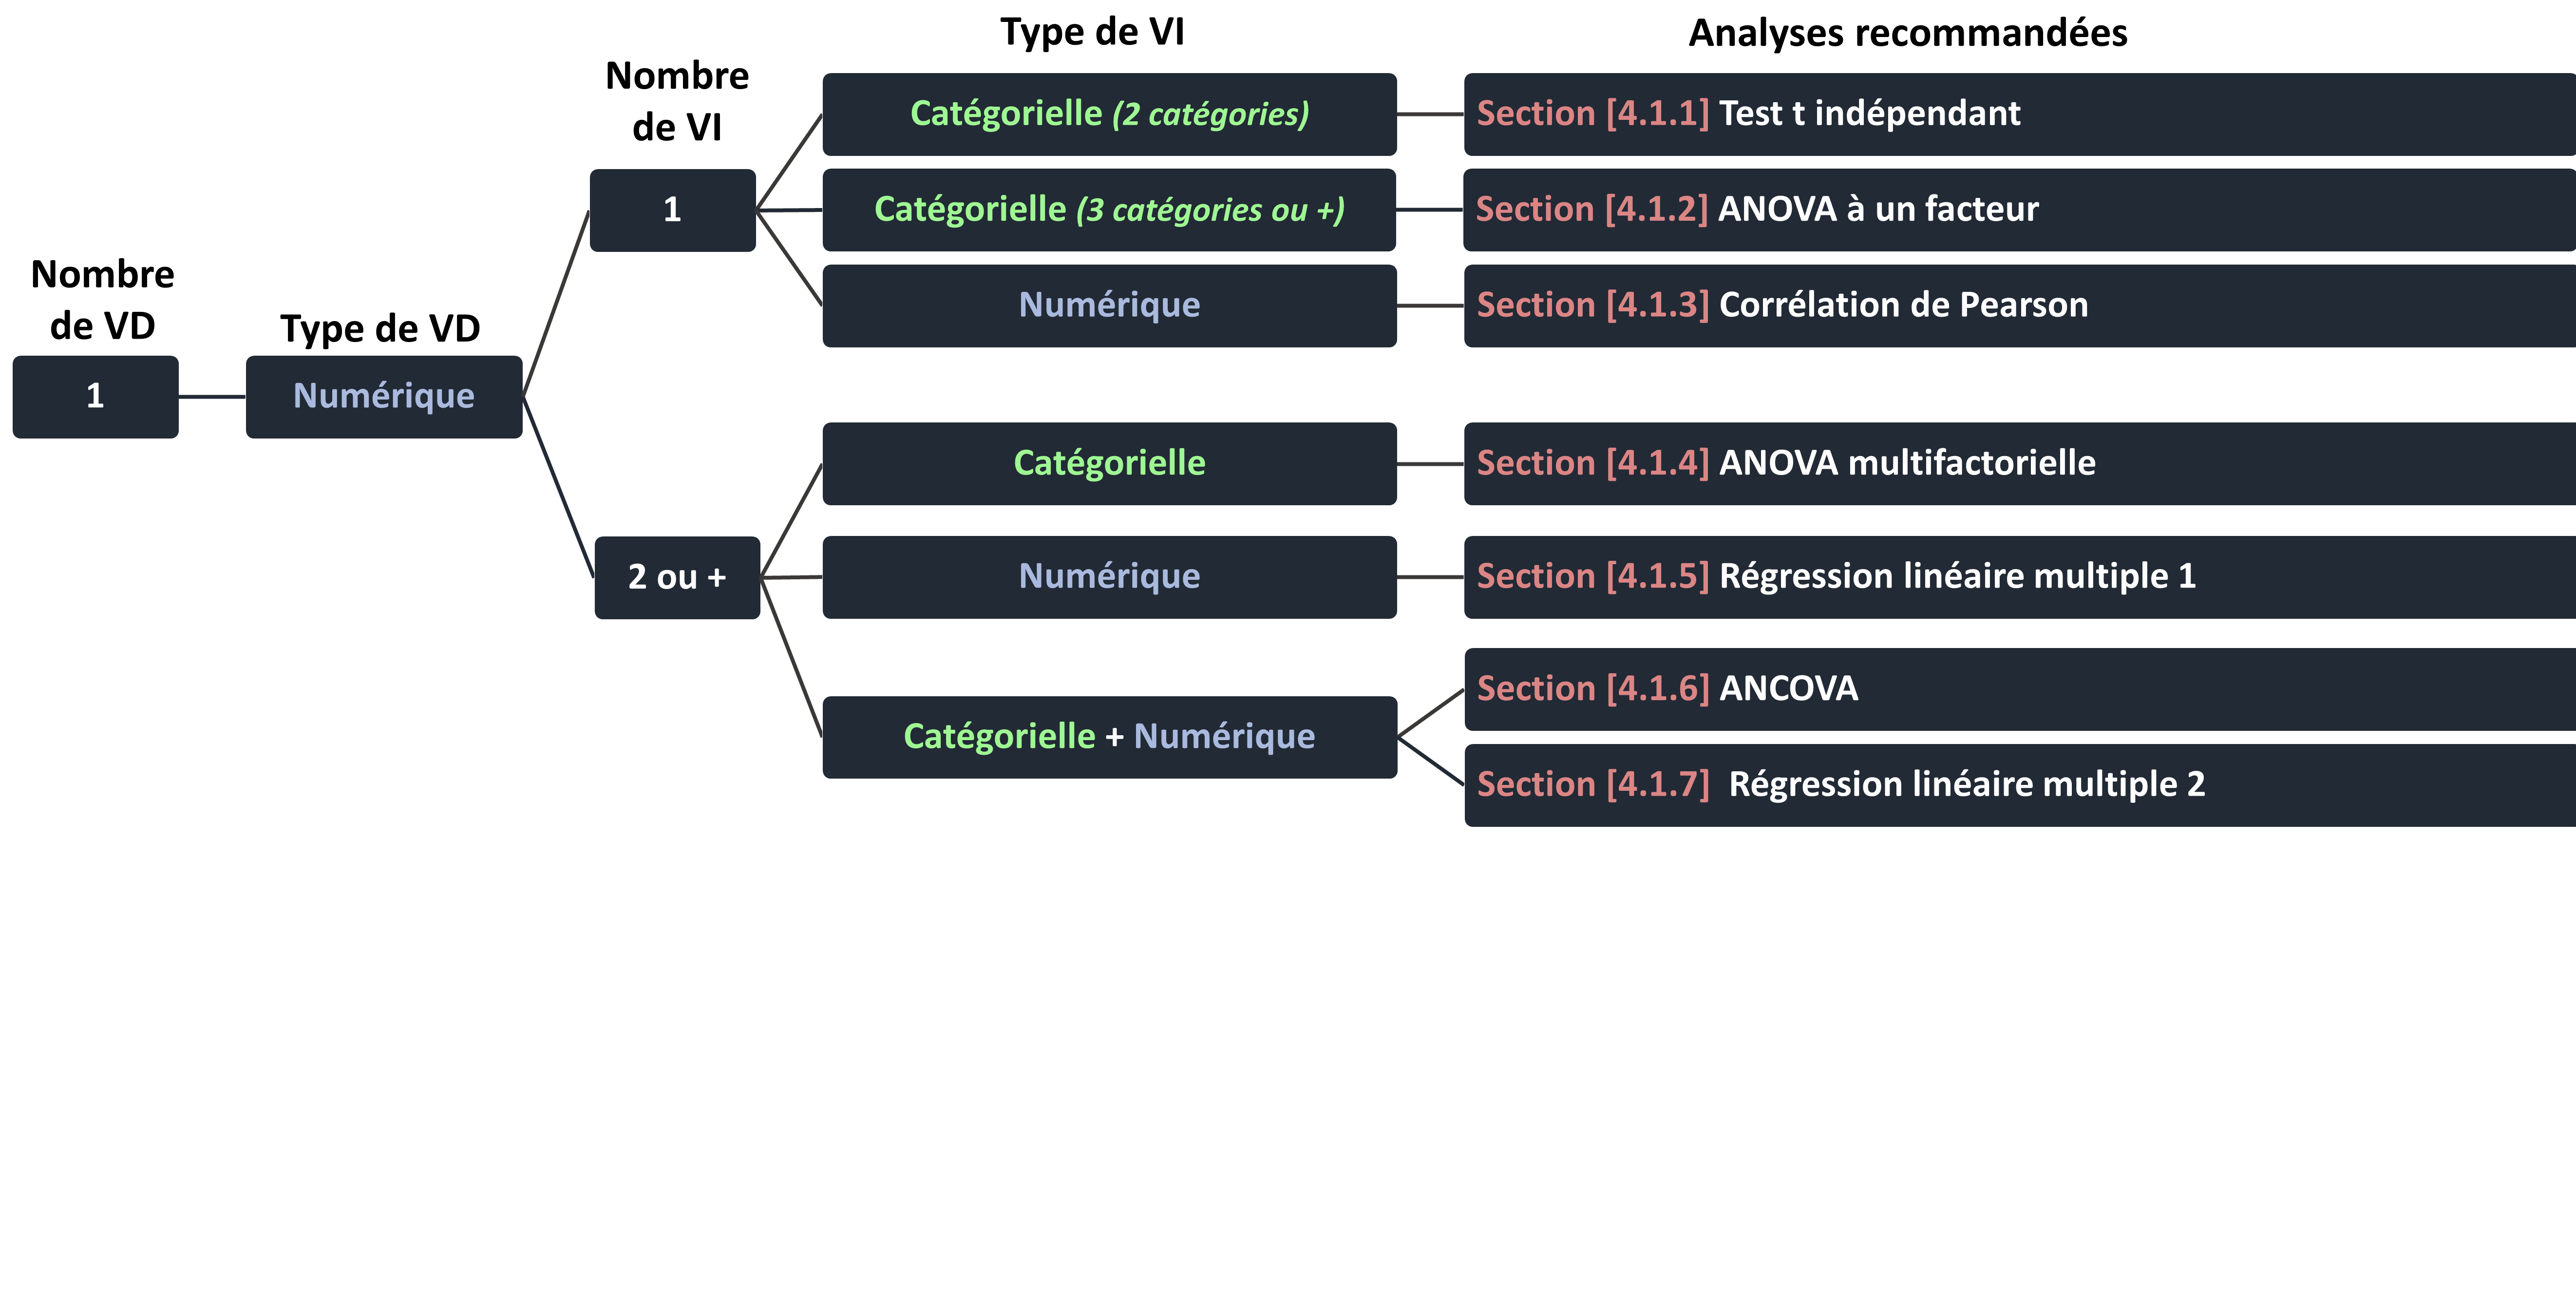
\includegraphics{/Users/coren/Documents/Manuel_R_independant/arbre1.png}

\textbf{Votre étude ne comporte qu'une seule mesure d'une VD catégorielle}

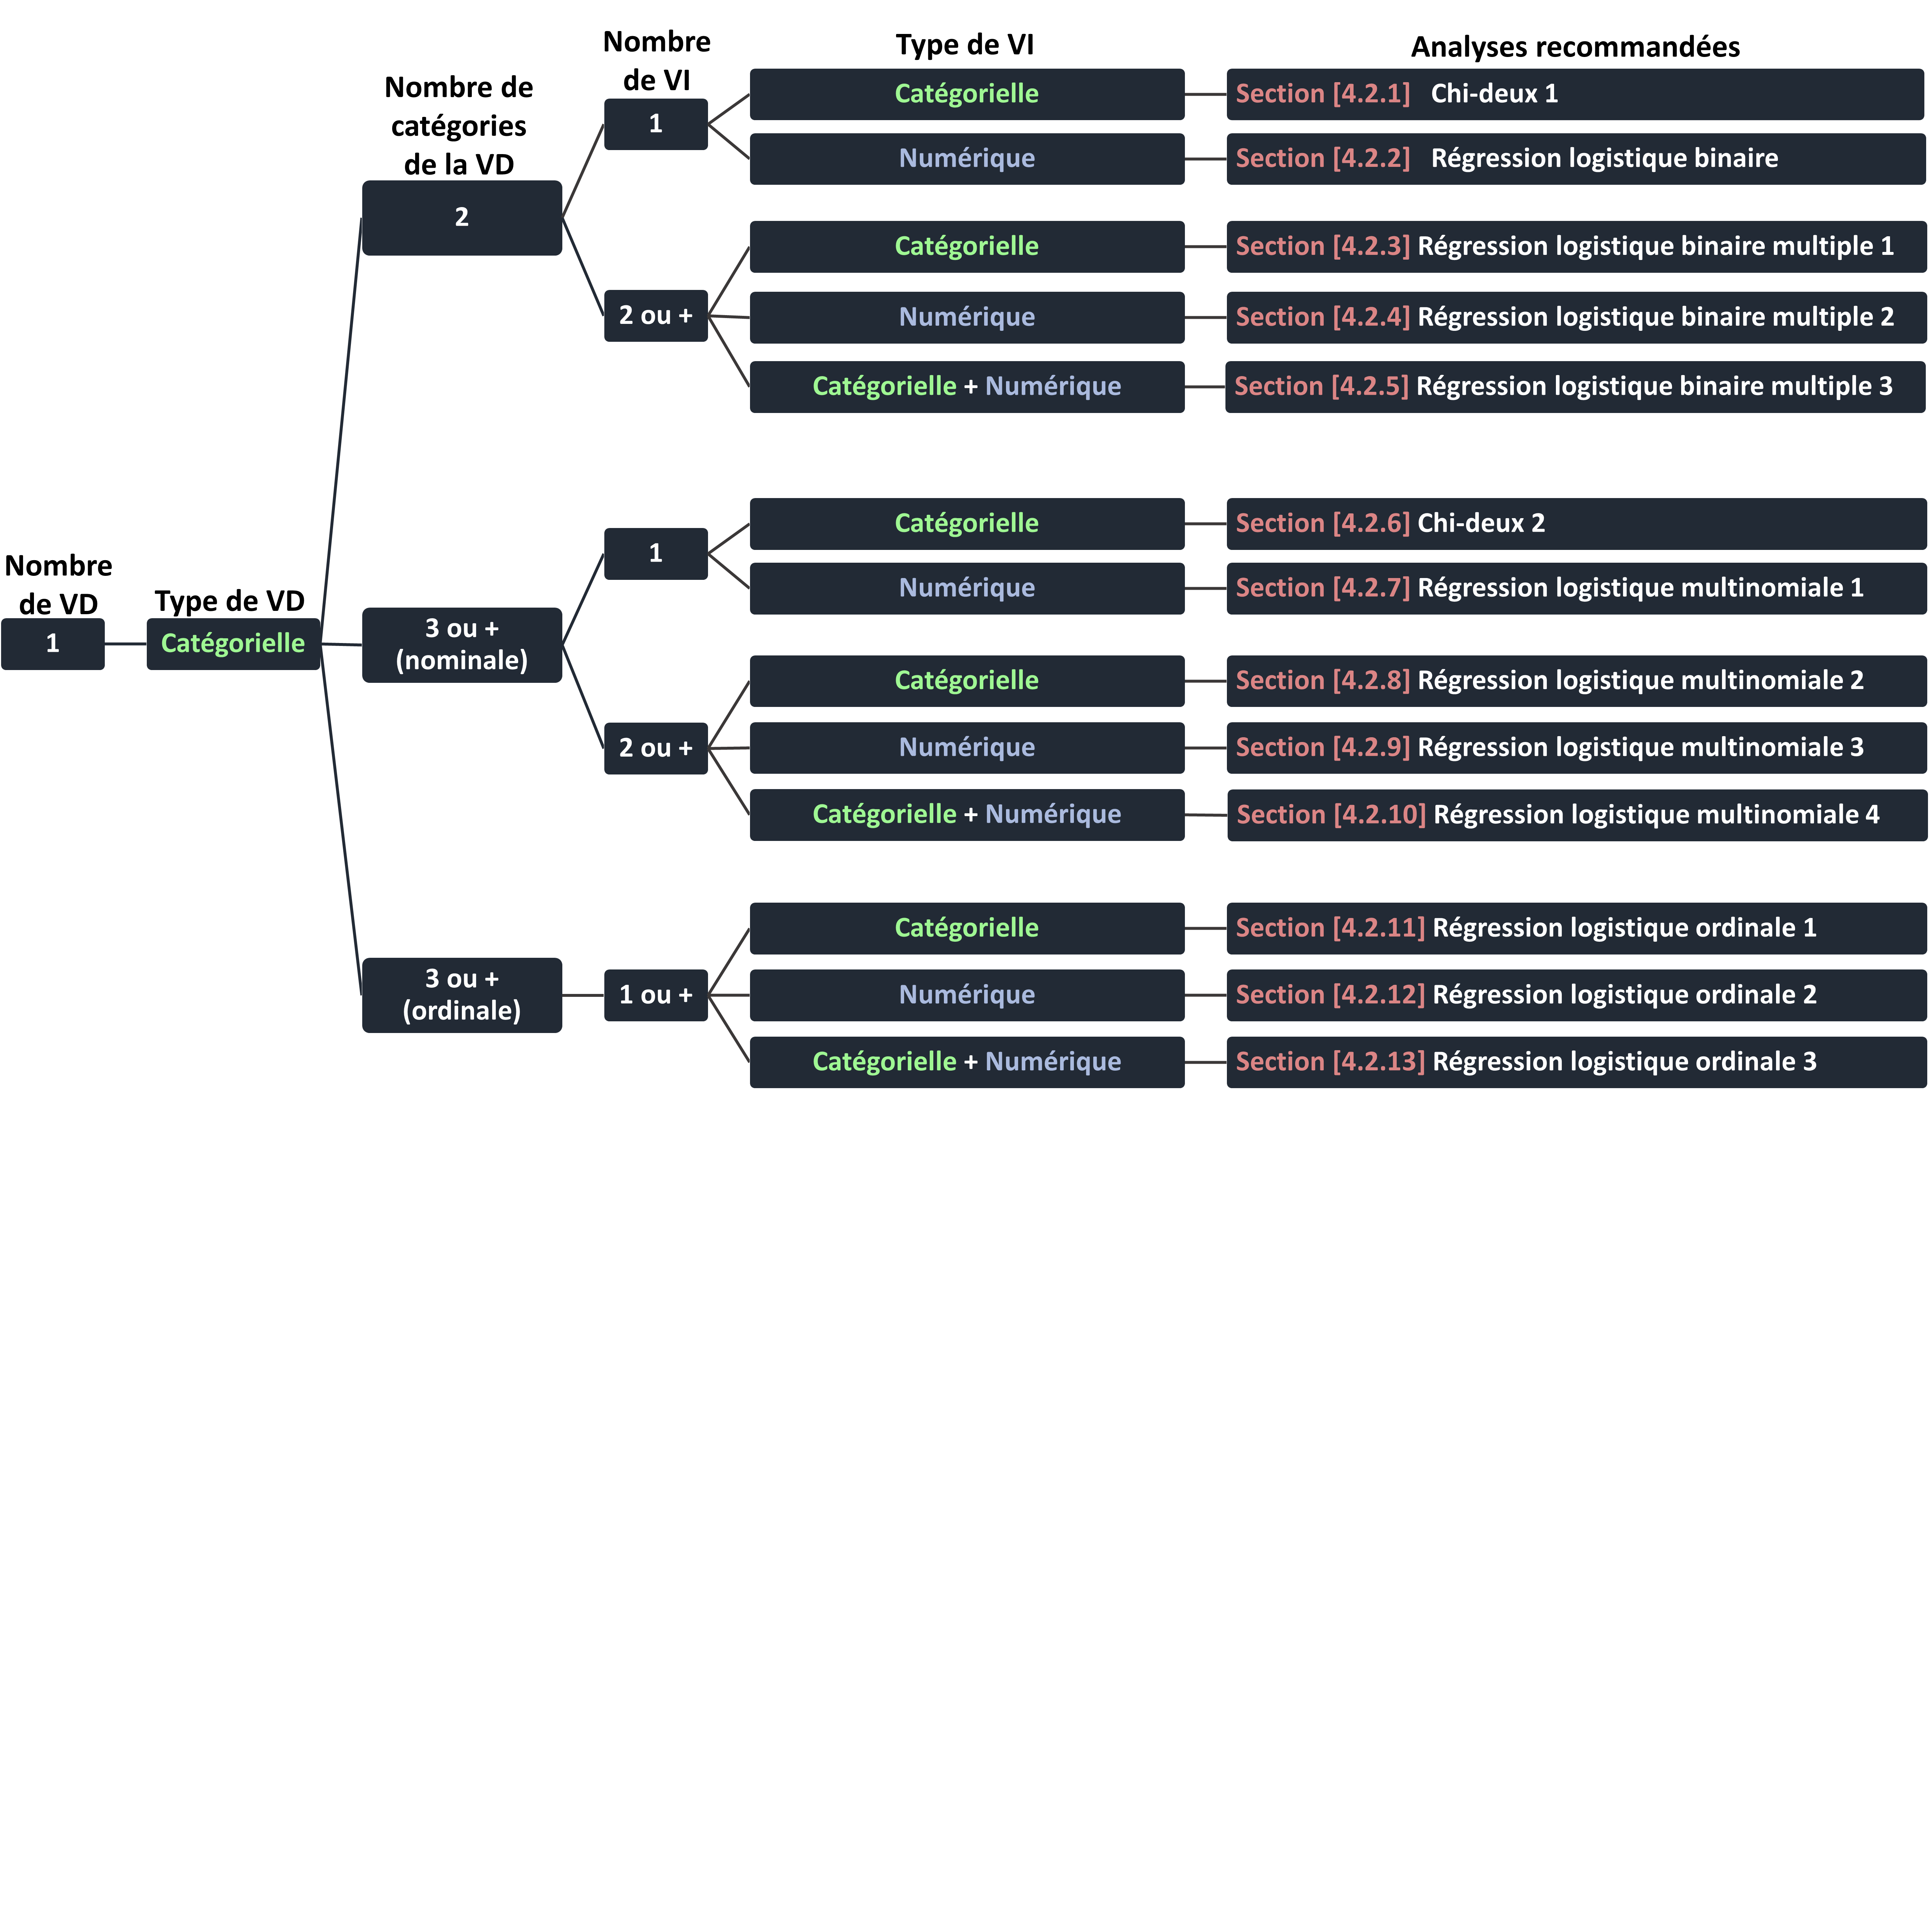
\includegraphics{/Users/coren/Documents/Manuel_R_independant/arbre2.png}

\textbf{Votre étude ne comporte qu'une seule mesure de plusieurs VD numériques}

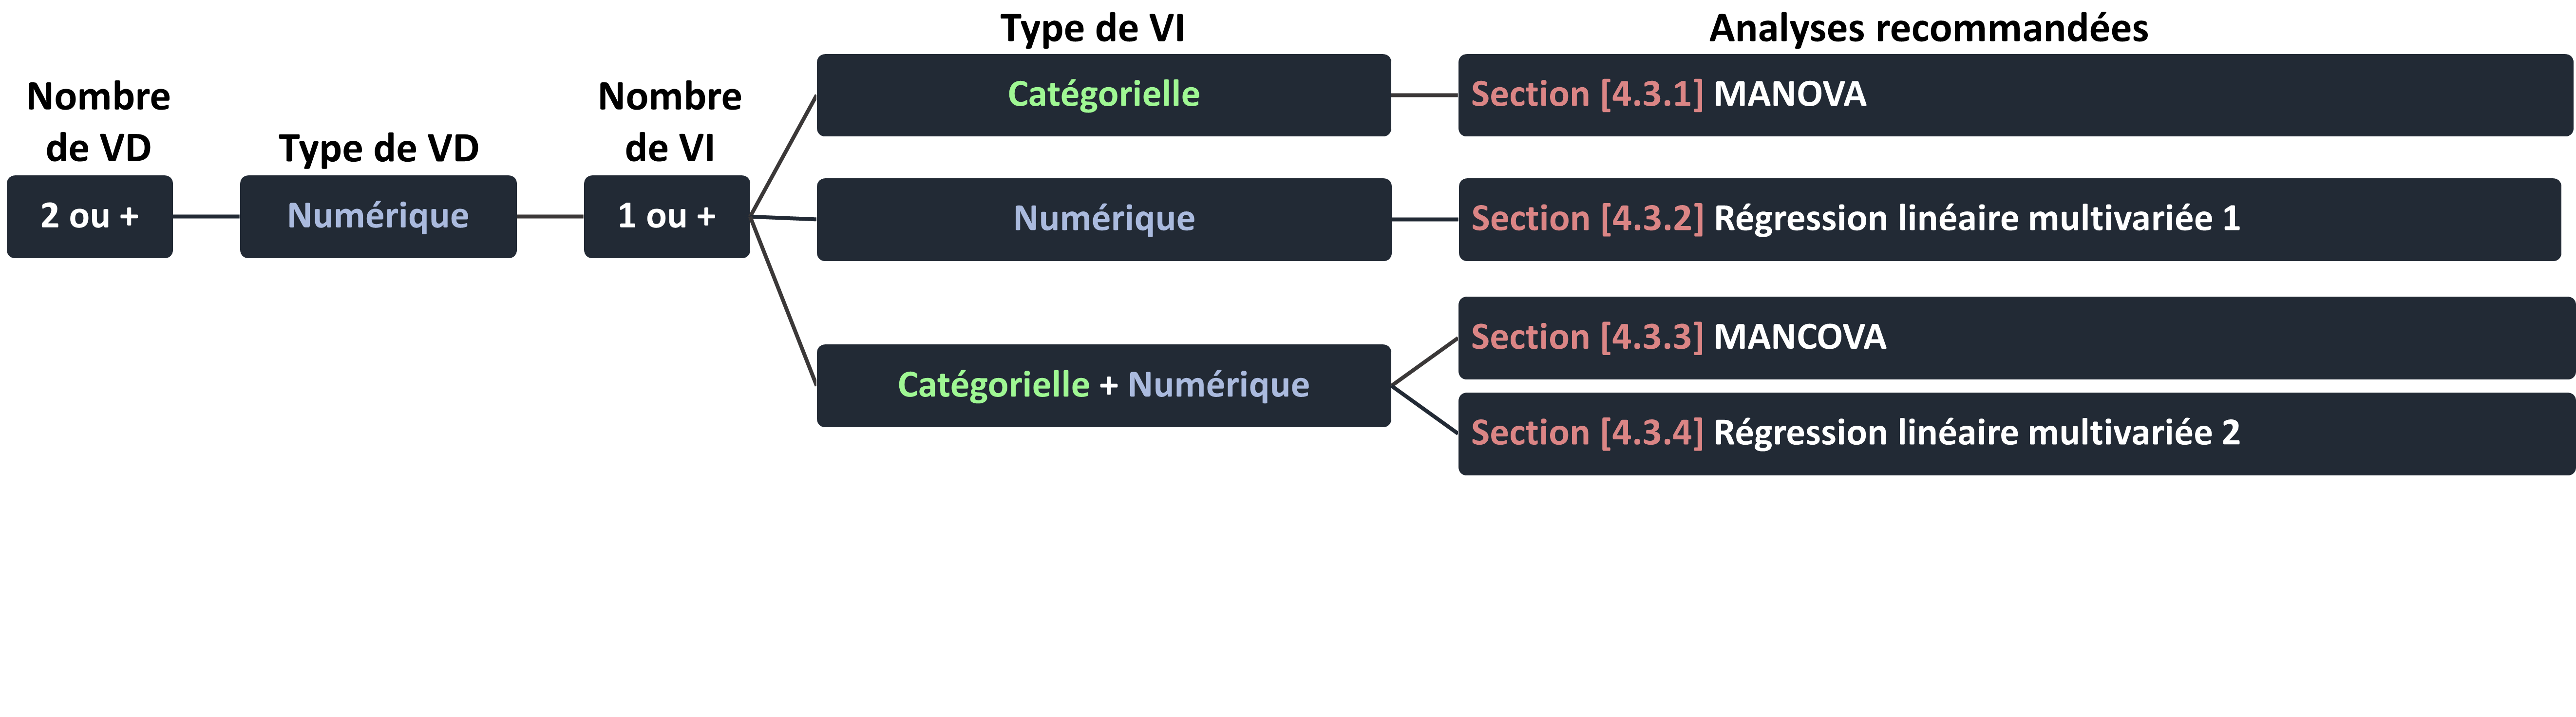
\includegraphics{/Users/coren/Documents/Manuel_R_independant/arbre3.png}

Une fois que vous avez sélectionné l'analyse statistique pertinente, reportez vous à la vignette correspondante (les numéros de section de chaque analyse sont indiqués dans les arbres décisionnels).
Le code sous-tendant chacune des étapes suivantes est systématiquement présenté au sein de chaque vignette.

\hypertarget{etape-3-charger-votre-fichier-de-donnuxe9es}{%
\section{Etape 3 : Charger votre fichier de données}\label{etape-3-charger-votre-fichier-de-donnuxe9es}}

Au début de chaque vignette, nous vous proposerons de charger votre fichier de données et de renommer les colonnes appropriées. \textbf{Cette étape n'est obligatoire que si vous souhaitez analyser vos propres données.} Si -- dans un premier temps -- vous souhaitez observer comment fonctionne le logiciel R, vous pouvez générer les données fictives. Chaque vignette comporte en effet un code permettant de générer des données fictives appropriées pour les analyses présentées dans la vignette (le code permettant de générer ces données fictives est donné au sein de la partie \textbf{Données fictives}). Ces données fictives n'ont pas d'autre but que de vous permettre d'appréhender simplement le fonctionnement de R.

Parfois, une étape relativement difficile dans R est d'arriver à charger son propre fichier de données. Afin de simplifier cette étape, une astuce est d'obliger R à ouvrir une fenêtre d'explorateur, afin que vous puissiez chercher votre fichier de données au sein de votre disque dur.

En fonction de vos besoins, copiez-collez la ligne de code dont vous avez besoin

\begin{Shaded}
\begin{Highlighting}[]
\CommentTok{# Si vous avez un fichier sauvegardé sous excel, commencez par charger la librairie du package `readxl` à l’aide de la commande suivante}
\KeywordTok{library}\NormalTok{(readxl) }
\NormalTok{my_data <-}\StringTok{ }\KeywordTok{read.delim}\NormalTok{(}\KeywordTok{file.choose}\NormalTok{()) }\CommentTok{#si vous avez un fichier .txt}
\NormalTok{my_data <-}\StringTok{ }\KeywordTok{read.csv}\NormalTok{(}\KeywordTok{file.choose}\NormalTok{()) }\CommentTok{#si vous avez un fichier .csv}
\NormalTok{my_data <-}\StringTok{ }\KeywordTok{read_excel}\NormalTok{(}\KeywordTok{file.choose}\NormalTok{()) }\CommentTok{#si vous avez un fichier .xls ou .xlsx}
\end{Highlighting}
\end{Shaded}

Si tout fonctionne bien, une fenêtre de l'explorateur devrait s'ouvrir et devrait vous permettre de localiser et d'ouvrir votre fichier de données facilement. Il arrive parfois que cette fenêtre s'ouvre en arrière-plan. Si aucune fenêtre d'exploration ne s'ouvre alors que vous avez entré une des commandes décrites, réduisez simplement la fenêtre de R ainsi que toutes vos autres fenêtres ouvertes. Vous trouverez cette fenêtre pour sélectionner votre fichier de données en arrière plan.
Une autre solution consiste à appuyer simultanément sur les touches ``alt+tab'' et de séletionner directement cette fenêtre.

\hypertarget{etape-4-duxe9clarer-le-type-de-variable}{%
\section{Etape 4 : Déclarer le type de variable}\label{etape-4-duxe9clarer-le-type-de-variable}}

R part de l'hypothèse selon laquelle toutes les variables contenant des chiffres sont des variables numériques et les variables contenants des caractères sont catégorielles. Une étape cruciale est donc de déclarer le type de chacune des variables impliquées dans les analyses.

Il existe deux types de variables catégorielles :

\textbf{1. Les variables nominales (ou facteurs)}
Les facteurs sont des variables dont les modalités ne peuvent pas être hiérarchisées. Par exemple, si vous vous intéressez aux types de pathologies mentales rencontrées par une population, vous obtiendrez une variable non-numérique, dont les modalités ne peuvent être hiérarchisées (e.g., « Schizophrénie », « Dépression », etc\ldots). Lorsqu'un facteur contient deux modalités, cette variable est généralement appelée une variable binaire ou dichotomique tandis qu'un facteur contenant plus de deux modalités est généralement appelé une variable multicatégorielle si c'est une variable indépendante ou multinomiale si c'est une variable dépendante.

\textbf{2. Les variables ordinales}
Lorsqu'une variable ne respecte pas les conditions d'une variable numérique mais dispose de catégories qui peuvent être hiérarchisées les unes avec les autres, cette variable est appelée une variable ordinale. Par exemple, si vous vous intéressez à l'influence du niveau académique des étudiants (Licence / Master / Doctorat) sur une variable dépendante, votre le niveau académique ne peut être considérée comme numérique mais dispose de modalités pouvant être hiérarchisées (les étudiants en Licence ayant un niveau académique plus faible que ceux en Master, etc\ldots).

\hypertarget{duxe9clarer-une-variable-en-tant-que-variable-nominale-facteur}{%
\subsection{Déclarer une variable en tant que variable nominale / facteur}\label{duxe9clarer-une-variable-en-tant-que-variable-nominale-facteur}}

Pour un jeu de données stocké sous le nom d'objet \texttt{my\_data} , déclarer une variable nommée \texttt{Variable1} en tant que facteur nécessite d'utiliser la commande :

\texttt{my\_data\$Variable1\ \textless{}-\ factor(my\_data\$Variable1)}

Pour rappel, le code \texttt{my\_data\$Variable1} permet de sélectionner la colonne ayant le nom Variable1 au sein du jeu de données nommé \texttt{my\_data}. Avec la commande ci-dessus, nous remplaçons la variable \texttt{Variable1} par la variable \texttt{Variable1} déclarée comme facteur. Libre à vous de stocker la variable Variable1 en tant que facteur sous un autre nom.
Par exemple :
\texttt{my\_data\$Variable1Facteur\textless{}-factor(my\_data\$Variable1)}

Dès lors, la nouvelle \texttt{Variable1Facteur} est égale à la variable \texttt{Variable1} déclarée comme facteur.

\hypertarget{duxe9clarer-une-variable-en-tant-que-variable-ordinale}{%
\subsection{Déclarer une variable en tant que variable ordinale}\label{duxe9clarer-une-variable-en-tant-que-variable-ordinale}}

Pour un jeu de données stocké sous le nom d'objet \texttt{my\_data} , déclarer une variable nommée \texttt{Variable1} en tant que variable ordinale nécessite d'utiliser la commande :

\texttt{my\_data\$Variable1\ \textless{}-\ ordered(my\_data\$Variable1)}

Pour rappel, le code \texttt{my\_data\$Variable1} permet de sélectionner la colonne ayant le nom Variable1 au sein du jeu de données nommé \texttt{my\_data}. Avec la commande ci-dessus, nous remplaçons la variable \texttt{Variable1} par la variable \texttt{Variable1} déclarée comme variable ordinale. Libre à vous de stocker la variable Variable1 en tant que variable ordinale sous un autre nom.
Par exemple :
\texttt{my\_data\$Variable1Ord\textless{}-ordered(my\_data\$Variable1)}

\hypertarget{duxe9clarer-une-variable-en-tant-que-variable-numuxe9rique}{%
\subsection{Déclarer une variable en tant que variable numérique}\label{duxe9clarer-une-variable-en-tant-que-variable-numuxe9rique}}

Pour un jeu de données stocké sous le nom d'objet \texttt{my\_data} , déclarer une variable nommée \texttt{Variable1} en tant que variable numérique nécessite d'utiliser la commande :

\texttt{my\_data\$Variable1\ \textless{}-\ as.numeric(as.character(my\_data\$Variable1))}

Pour rappel, le code \texttt{my\_data\$Variable1} permet de sélectionner la colonne ayant le nom Variable1 au sein du jeu de données nommé \texttt{my\_data}. Avec la commande ci-dessus, nous remplaçons la variable \texttt{Variable1} par la variable \texttt{Variable1} déclarée comme variable numérique. Libre à vous de stocker la variable Variable1 en tant que variable numérique sous un autre nom.
Par exemple :
\texttt{my\_data\$Variable1Num\textless{}-as.numeric(as.character(my\_data\$Variable1))}

\hypertarget{etape-5-inspecter-les-donnuxe9es-et-la-distribution-de-vos-variables}{%
\section{Etape 5 : Inspecter les données et la distribution de vos variables}\label{etape-5-inspecter-les-donnuxe9es-et-la-distribution-de-vos-variables}}

R n'ayant pas d'interface graphique, il est très important de visualiser les données chargées. Soit \texttt{my\_data} un jeu de données comprenant 4 variables (80 observations)

\begin{itemize}
\tightlist
\item
  la variable VD1.cont est une variable dépendante numérique
\item
  la variable VI1.cont est une variable indépendante numérique
\item
  la variable VI2.cat est une variable indépendante catégorielle
\item
  la variable VI3.cat est une variable indépendante catégorielle
\end{itemize}

Pour visualiser l'ensemble de votre jeu de données, il vous suffit de rentrer, dans la console de R :

\begin{itemize}
\tightlist
\item
  \texttt{View(my\_data)} pour voir l'ensemble de votre jeu de données
\item
  \texttt{head(my\_data)} pour voir les premières lignes de votre jeu de données
\item
  \texttt{tail(my\_data)} pour voir les dernières lignes de votre jeu de données
\end{itemize}

\textbf{Utilisation du package GGally pour inspecter ses données}
Une inspection visuelle de la distribution de vos variables et de leurs associations deux-à-deux est possible facilement grâce à un package : \texttt{GGally}. Nous vous décrivons un exemple afin de vous familiariser avec les sorties de ce package

\begin{Shaded}
\begin{Highlighting}[]
\KeywordTok{library}\NormalTok{(GGally)}
\KeywordTok{ggpairs}\NormalTok{(}\DataTypeTok{data =}\NormalTok{ my_data,}
        \DataTypeTok{lower =} \KeywordTok{list}\NormalTok{(}\DataTypeTok{continuous =} \KeywordTok{wrap}\NormalTok{(}\StringTok{"smooth"}\NormalTok{, }\DataTypeTok{alpha =} \FloatTok{0.7}\NormalTok{), }\DataTypeTok{combo =} \StringTok{"box_no_facet"}\NormalTok{),}
        \DataTypeTok{upper =} \KeywordTok{list}\NormalTok{(}\DataTypeTok{combo =} \StringTok{"facetdensity"}\NormalTok{, }\DataTypeTok{discrete =} \StringTok{"facetbar"}\NormalTok{), }
        \DataTypeTok{mapping =} \KeywordTok{aes}\NormalTok{(}\DataTypeTok{alpha =} \FloatTok{0.8}\NormalTok{)) }\OperatorTok{+}\StringTok{ }\KeywordTok{theme_bw}\NormalTok{()}
\end{Highlighting}
\end{Shaded}

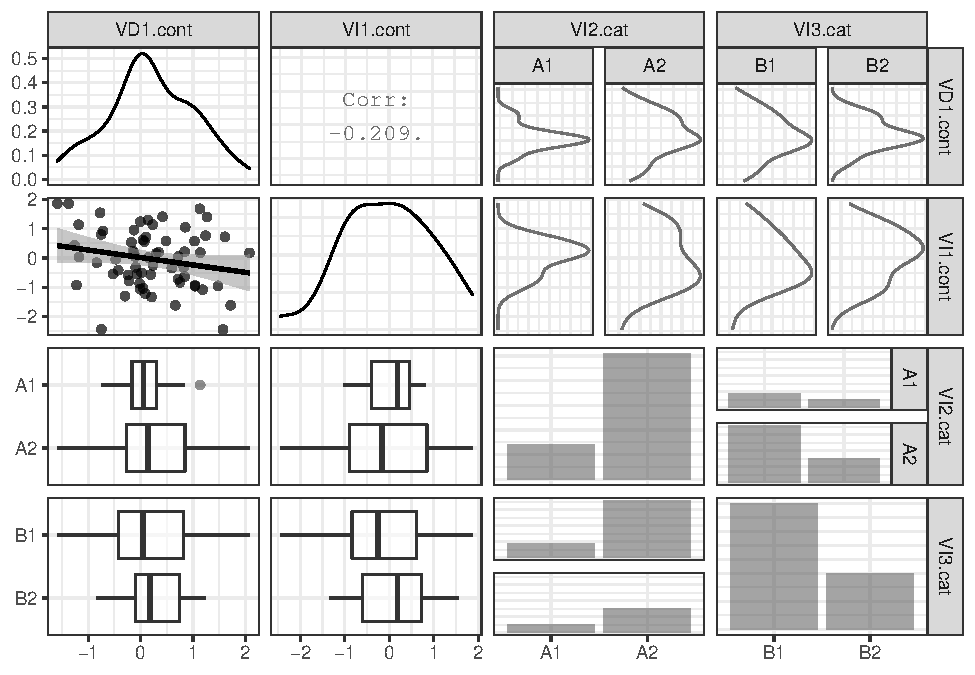
\includegraphics{Manuel_R_independant_files/figure-latex/unnamed-chunk-6-1.pdf}

\begin{enumerate}
\def\labelenumi{\arabic{enumi}.}
\item
  Au niveau de la diagonale, les graphiques représentent la ditrisbution des variables. Les variables numériques sont représentées sous la forme d'une densité tandis que les variables catégorielles sont représentées sous la forme d'un diagramme en bâton.
\item
  Au dessus et en dessous de la diagonale, les graphiques représentent les associations deux-à-deux entre chacune des variables.
\end{enumerate}

\begin{itemize}
\tightlist
\item
  \emph{Au-dessus de la diagonale:}

  \begin{itemize}
  \tightlist
  \item
    les associations entre 2 variables numériques sont représentées par leur coefficient de corrélation.
  \item
    les associations entre une variable catégorielle et une variable numérique sont représentées sous la forme d'une courbe de densité de la variable numérique pour chaque modalité de la variable catégorielle.
  \item
    les associations entre deux variables catégorielles sont représentées par le diagramme en batôn d'une variable catégorielle pour chaque modalité de l'autre variable.
  \end{itemize}
\item
  \emph{En-dessous de la diagonale:}

  \begin{itemize}
  \tightlist
  \item
    les associations entre 2 variables numériques sont représentées sous la forme d'un nuage de points (la droite représente la pente de la corrélation).
  \item
    les associations entre une variable catégorielle et une variable numérique sont représentées sous la forme d'un diagramme en boîte.
  \item
    les associations entre deux variables catégorielles sont représentées par le diagramme en batôn d'une variable catégorielle pour chaque modalité de l'autre variable.
  \end{itemize}
\end{itemize}

Pour adapter cette commande à votre propre jeu de données, la seule modification à effectuer est de remplacer \texttt{data\ =\ my\_data} par \texttt{data\ =\ le.nom.de.votre.propre.jeu.de.données}

\hypertarget{etape-6-ruxe9aliser-votre-analyse-statistique-et-obtenir-des-tailles-deffet-etou-tests-post-hoc}{%
\section{Etape 6 : Réaliser votre analyse statistique et obtenir des tailles d'effet et/ou tests-post-hoc}\label{etape-6-ruxe9aliser-votre-analyse-statistique-et-obtenir-des-tailles-deffet-etou-tests-post-hoc}}

Cette étape ne demande que de copier et coller le code décrit dans la partie \textbf{Analyse des données} présente dans chaque vignette.

\hypertarget{vous-nuxeates-pas-habituuxe9-aux-sorties-de-ruxe9sultats-guxe9nuxe9ruxe9es-par-r}{%
\subsection{Vous n'êtes pas habitué aux sorties de résultats générées par R}\label{vous-nuxeates-pas-habituuxe9-aux-sorties-de-ruxe9sultats-guxe9nuxe9ruxe9es-par-r}}

Nous vous conseillons de vous familiariser avec les sorties de résultats générées par R grâce aux données fictives associées à la partie « Interprétation » présentent dans chaque vignette.

Ces données fictives comportent :

\begin{itemize}
\tightlist
\item
  une ou plusieurs variables indépendantes. Si elles sont de type numérique, elles sont appelées VI.cont. Si elles sont de type catégoriel, elle sont appelées VI.cat (si elles comportent 2 catégories), VI.multicat (si elles comportement plus de 3 catégories) et VI.ord (si elles sont ordinales).
\item
  une ou plusieurs variables dépendantes. Si elles sont de type numérique, elles sont appelées VD.cont. Si elles sont de type catégoriel, elle sont appelées VD.cat (si elles comportent 2 catégories), VD.multicat (si elles comportement plus de 3 catégories) et VD.ord (si elles sont ordinales).
\end{itemize}

Une fois ces données fictivités générées il vous suffit de :

\begin{itemize}
\tightlist
\item
  Réaliser les analyses grâce au code fourni dans la partie \textbf{Analyse des données}
\item
  Générer la sortie graphique associée afin d'avoir une représentation visuelle des données grâce à la partie \textbf{Graphique}
\item
  Comparer la sortie de R aux résultats décrits dans la partie \textbf{Interprétation} présente dans chaque vignette. Les valeurs décrites dans la partie interprétation correspondent aux résultats produits par l'analyse des données fictives.
\end{itemize}

\hypertarget{vous-uxeates-habituuxe9-aux-sorties-de-ruxe9sultats-guxe9nuxe9ruxe9es-par-r}{%
\subsection{Vous êtes habitué aux sorties de résultats générées par R}\label{vous-uxeates-habituuxe9-aux-sorties-de-ruxe9sultats-guxe9nuxe9ruxe9es-par-r}}

Chargez votre fichier de données grâce aux commandes fournies dans la partie \textbf{Données réelles} et adaptez simplement le code des parties \textbf{Inspection des données}, \textbf{Analyse des données} et \textbf{Graphique} de la vignette correspondant à votre analyse au besoin. Lorsque vous souhaitez appliquer le code directement à vos données, il n'est pas nécessaire de générer les données fictives, et la partie interprétation ne vous sera pas utile.

\hypertarget{etape-7-obtenir-une-repruxe9sentation-graphique}{%
\section{Etape 7 : Obtenir une représentation graphique}\label{etape-7-obtenir-une-repruxe9sentation-graphique}}

Le code de la partie ``Graphique'' permet d'avoir une représentation graphique de vos données, fournissant ainsi une aide visuelle à l'interprétation de vos données.

\hypertarget{ruxe9alisation-des-analyses-statistiques}{%
\chapter{Réalisation des analyses statistiques}\label{ruxe9alisation-des-analyses-statistiques}}

Les vignettes suivantes décrivent la façon d'implanter différentes analyses statistiques. Reportez-vous au numéro de vignette indiqué par l'arbre décisionnel afin d'avoir un exemple de l'analyse statistique dont vous avez besoin.

Pour rappel, si jamais vous devez adapter le code ci-dessous pour construire un modèle statistique différent de celui rapporté, voici la syntaxe adoptée par R :

\begin{Shaded}
\begin{Highlighting}[]
\NormalTok{formula =}\StringTok{ }\NormalTok{y }\OperatorTok{~}\StringTok{ }\NormalTok{x }\CommentTok{# effet principal de x sur y }
\NormalTok{formula =}\StringTok{ }\NormalTok{y }\OperatorTok{~}\StringTok{ }\NormalTok{x }\OperatorTok{+}\StringTok{ }\NormalTok{z }\CommentTok{# effets principaux de x et z sur y }
\NormalTok{formula =}\StringTok{ }\NormalTok{y }\OperatorTok{~}\StringTok{ }\NormalTok{x }\OperatorTok{+}\StringTok{ }\NormalTok{z }\OperatorTok{+}\StringTok{ }\NormalTok{m }\CommentTok{# effets principaux de x, z et m sur y }
\NormalTok{formula =}\StringTok{ }\NormalTok{y }\OperatorTok{~}\StringTok{ }\NormalTok{x }\OperatorTok{+}\StringTok{ }\NormalTok{z }\OperatorTok{+}\StringTok{ }\NormalTok{m }\OperatorTok{+}\StringTok{ }\NormalTok{x}\OperatorTok{:}\NormalTok{z }\CommentTok{# effets principaux de x, z et m sur y et interaction entre x et z sur y}
\NormalTok{formula =}\StringTok{ }\NormalTok{y }\OperatorTok{~}\StringTok{ }\NormalTok{x}\OperatorTok{*}\NormalTok{z }\OperatorTok{+}\StringTok{ }\NormalTok{m }\CommentTok{# commande strictement équivalente à la ligne précédente}
\NormalTok{formula =}\StringTok{ }\NormalTok{y }\OperatorTok{~}\StringTok{ }\NormalTok{x }\OperatorTok{+}\StringTok{ }\NormalTok{z }\OperatorTok{+}\StringTok{ }\NormalTok{m }\OperatorTok{+}\StringTok{ }\NormalTok{x}\OperatorTok{:}\NormalTok{z }\OperatorTok{+}\StringTok{ }\NormalTok{x}\OperatorTok{:}\NormalTok{m }\OperatorTok{+}\StringTok{ }\NormalTok{m}\OperatorTok{:}\NormalTok{z }\OperatorTok{+}\StringTok{ }\NormalTok{x}\OperatorTok{:}\NormalTok{z}\OperatorTok{:}\NormalTok{m }\CommentTok{# analyse de tous les effets principaux, des 3 interactions simples et de l'interaction double sur y}
\NormalTok{formula =}\StringTok{ }\NormalTok{y }\OperatorTok{~}\StringTok{ }\NormalTok{x}\OperatorTok{*}\NormalTok{m}\OperatorTok{*}\NormalTok{z }\CommentTok{# commande strictement équivalente à la ligne précédente}
\end{Highlighting}
\end{Shaded}

\hypertarget{une-seule-vd-numuxe9rique}{%
\section{Une seule VD numérique}\label{une-seule-vd-numuxe9rique}}

\hypertarget{test-t-induxe9pendant}{%
\subsection{Test t indépendant}\label{test-t-induxe9pendant}}

\hypertarget{type-de-variables}{%
\subsubsection{Type de variables}\label{type-de-variables}}

\textbf{Variable Dépendante :} Numérique
\textbf{Variable Indépendante :} Catégorielle (2 catégories)

\hypertarget{packages-nuxe9cessaires}{%
\subsubsection{Packages nécessaires}\label{packages-nuxe9cessaires}}

\begin{Shaded}
\begin{Highlighting}[]
\KeywordTok{library}\NormalTok{(ggplot2)}
\KeywordTok{library}\NormalTok{(GGally)}
\KeywordTok{library}\NormalTok{(forcats)}
\KeywordTok{library}\NormalTok{(dplyr)}
\KeywordTok{library}\NormalTok{(rstatix)}
\KeywordTok{library}\NormalTok{(readxl)}
\end{Highlighting}
\end{Shaded}

\hypertarget{donnuxe9es-ruxe9elles}{%
\subsubsection{Données réelles}\label{donnuxe9es-ruxe9elles}}

\begin{Shaded}
\begin{Highlighting}[]
\CommentTok{# choisissez la ligne appropriée au format de votre fichier de données. }

\CommentTok{# si vos données sont dans un fichier .txt}
\NormalTok{my_data.ttest <-}\StringTok{ }\KeywordTok{read.delim}\NormalTok{(}\KeywordTok{file.choose}\NormalTok{())}

\CommentTok{# si vos données sont dans un fichier .csv}
\NormalTok{my_data.ttest <-}\StringTok{ }\KeywordTok{read.csv}\NormalTok{(}\KeywordTok{file.choose}\NormalTok{())}

\CommentTok{# si vos données sont dans un fichier .xls / .xlsx}
\NormalTok{my_data.ttest <-}\StringTok{ }\KeywordTok{read_excel}\NormalTok{(}\KeywordTok{file.choose}\NormalTok{())}

\CommentTok{# une fois vos données chargées, vous pouvez renommer vos noms de colonnes afin qu'ils correspondent à ceux utilisés dans le code ci-dessous}
\CommentTok{# Si vous ne souhaitez pas renommer vos noms de colonnes, sautez cette étape mais adaptez le code des parties suivantes en lui indiquant les noms de colonnes de vos données.}

\CommentTok{# On crée une nouvelle colonne pour votre variable dépendante continue (remplacez 'votre.nom.de.colonne' par le nom approprié)}
\NormalTok{my_data.ttest}\OperatorTok{$}\NormalTok{VD1.cont <-}\StringTok{ }\NormalTok{my_data.ttest}\OperatorTok{$}\StringTok{'votre.nom.de.colonne'}

\CommentTok{# On crée une nouvelle colonne pour votre variable indépendante catégorielle (remplacez 'votre.nom.de.colonne' par le nom approprié)}
\NormalTok{my_data.ttest}\OperatorTok{$}\NormalTok{VI1.cat <-}\StringTok{ }\NormalTok{my_data.ttest}\OperatorTok{$}\StringTok{'votre.nom.de.colonne'}
\end{Highlighting}
\end{Shaded}

\hypertarget{donnuxe9es-fictives}{%
\subsubsection{Données fictives}\label{donnuxe9es-fictives}}

\begin{Shaded}
\begin{Highlighting}[]
\KeywordTok{set.seed}\NormalTok{(}\DecValTok{4321}\NormalTok{)}
\NormalTok{my_data.ttest <-}\StringTok{ }\KeywordTok{data.frame}\NormalTok{(}
  \DataTypeTok{VD1.cont =} \KeywordTok{rnorm}\NormalTok{(}\DecValTok{30}\NormalTok{),}
  \DataTypeTok{VI1.cat =} \KeywordTok{rep}\NormalTok{(}\KeywordTok{c}\NormalTok{(}\DecValTok{1}\NormalTok{, }\DecValTok{2}\NormalTok{), }\DataTypeTok{each =} \DecValTok{15}\NormalTok{))}

\CommentTok{# On renomme les catégories de VI1.cat pour que les résultats soient plus lisibles}
\NormalTok{my_data.ttest}\OperatorTok{$}\NormalTok{VI1.cat <-}\StringTok{ }\KeywordTok{fct_recode}\NormalTok{(}\KeywordTok{factor}\NormalTok{(my_data.ttest}\OperatorTok{$}\NormalTok{VI1.cat), }
                                 \StringTok{"Groupe 1"}\NormalTok{ =}\StringTok{ "1"}\NormalTok{, }
                                 \StringTok{"Groupe 2"}\NormalTok{ =}\StringTok{ "2"}\NormalTok{) }
\end{Highlighting}
\end{Shaded}

\hypertarget{duxe9claration-du-type-de-variable}{%
\subsubsection{Déclaration du type de variable}\label{duxe9claration-du-type-de-variable}}

\begin{Shaded}
\begin{Highlighting}[]
\NormalTok{my_data.ttest}\OperatorTok{$}\NormalTok{VD1.cont <-}\StringTok{ }\KeywordTok{as.numeric}\NormalTok{(}\KeywordTok{as.character}\NormalTok{(my_data.ttest}\OperatorTok{$}\NormalTok{VD1.cont))}
\NormalTok{my_data.ttest}\OperatorTok{$}\NormalTok{VI1.cat <-}\StringTok{ }\KeywordTok{factor}\NormalTok{(my_data.ttest}\OperatorTok{$}\NormalTok{VI1.cat)}
\end{Highlighting}
\end{Shaded}

\hypertarget{inspection-visuelle-des-donnuxe9es}{%
\subsubsection{Inspection visuelle des données}\label{inspection-visuelle-des-donnuxe9es}}

\begin{Shaded}
\begin{Highlighting}[]
\CommentTok{## Les graphiques situés sur la diagonale représentent la distribution des variables}
\CommentTok{## Les graphiques (ou les valeurs de corrélation) situés au dessus et en dessous de la diagonale représentent les associations deux-à-deux}
\KeywordTok{ggpairs}\NormalTok{(my_data.ttest,}
        \DataTypeTok{lower =} \KeywordTok{list}\NormalTok{(}\DataTypeTok{continuous =} \KeywordTok{wrap}\NormalTok{(}\StringTok{"smooth"}\NormalTok{, }\DataTypeTok{alpha =} \FloatTok{0.7}\NormalTok{), }\DataTypeTok{combo =} \StringTok{"box_no_facet"}\NormalTok{),}
        \DataTypeTok{upper =} \KeywordTok{list}\NormalTok{(}\DataTypeTok{combo =} \StringTok{"facetdensity"}\NormalTok{, }\DataTypeTok{discrete =} \StringTok{"facetbar"}\NormalTok{), }
        \DataTypeTok{mapping =} \KeywordTok{aes}\NormalTok{(}\DataTypeTok{alpha =} \FloatTok{0.8}\NormalTok{)) }\OperatorTok{+}\StringTok{ }\KeywordTok{theme_bw}\NormalTok{()}
\end{Highlighting}
\end{Shaded}

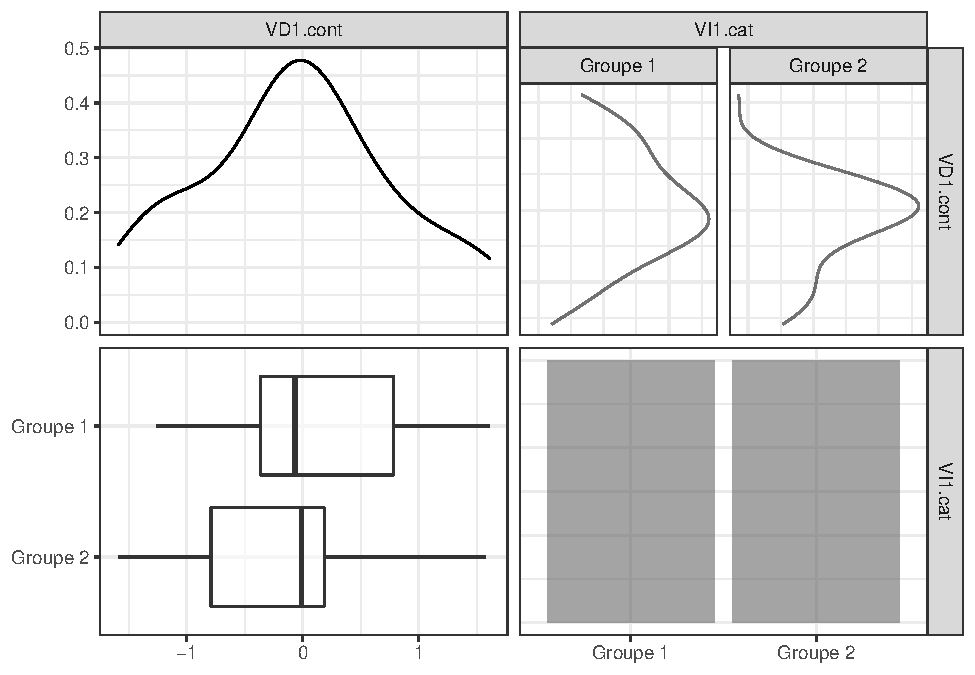
\includegraphics{Manuel_R_independant_files/figure-latex/unnamed-chunk-12-1.pdf}

\hypertarget{analyse-des-donnuxe9es}{%
\subsubsection{Analyse des données}\label{analyse-des-donnuxe9es}}

\begin{Shaded}
\begin{Highlighting}[]
\CommentTok{# calcul du test t et stockage des résultats dans l’objet t.test}
\NormalTok{t.test <-}\StringTok{ }\KeywordTok{t.test}\NormalTok{(}\DataTypeTok{formula =}\NormalTok{ VD1.cont }\OperatorTok{~}\StringTok{ }\NormalTok{VI1.cat, }
                 \DataTypeTok{data =}\NormalTok{ my_data.ttest,}
                 \DataTypeTok{var.equal =} \OtherTok{TRUE}\NormalTok{)}

\CommentTok{# calcul des moyennes et écarts types pour les deux modalités de VI.cat}
\NormalTok{description.ttest <-}\StringTok{ }\NormalTok{my_data.ttest }\OperatorTok\StringTok{ }
\StringTok{  }\KeywordTok{group_by}\NormalTok{(VI1.cat) }\OperatorTok\StringTok{ }
\StringTok{  }\KeywordTok{summarise}\NormalTok{(}
    \DataTypeTok{Mean =} \KeywordTok{mean}\NormalTok{(VD1.cont),}
    \DataTypeTok{SD =} \KeywordTok{sd}\NormalTok{(VD1.cont),}
    \DataTypeTok{N =} \KeywordTok{n}\NormalTok{())}

\CommentTok{# calcul de la taille d'effet de VI1.cat sur VD1.cont (SMD / d de cohen)}
\NormalTok{cohensd.ttest <-}\StringTok{ }\NormalTok{rstatix}\OperatorTok{::}\KeywordTok{cohens_d}\NormalTok{(}\DataTypeTok{data =}\NormalTok{ my_data.ttest,}
                    \DataTypeTok{formula =}\NormalTok{ VD1.cont }\OperatorTok{~}\StringTok{ }\NormalTok{VI1.cat, }
                    \DataTypeTok{var.equal =} \OtherTok{TRUE}\NormalTok{)}

\CommentTok{# obtention des différentes moyennes/écarts-types }
\NormalTok{description.ttest}
\end{Highlighting}
\end{Shaded}

\begin{verbatim}
## # A tibble: 2 x 4
##   VI1.cat    Mean    SD     N
##   <fct>     <dbl> <dbl> <int>
## 1 Groupe 1  0.116 0.868    15
## 2 Groupe 2 -0.200 0.831    15
\end{verbatim}

\begin{Shaded}
\begin{Highlighting}[]
\CommentTok{# obtention des résultats du test t }
\NormalTok{t.test}
\end{Highlighting}
\end{Shaded}

\begin{verbatim}
## 
## 	Two Sample t-test
## 
## data:  VD1.cont by VI1.cat
## t = 1.0194, df = 28, p-value = 0.3167
## alternative hypothesis: true difference in means is not equal to 0
## 95 percent confidence interval:
##  -0.3192537  0.9518066
## sample estimates:
## mean in group Groupe 1 mean in group Groupe 2 
##              0.1162924             -0.1999841
\end{verbatim}

\begin{Shaded}
\begin{Highlighting}[]
\CommentTok{# obtention de la taille d'effet}
\NormalTok{cohensd.ttest}
\end{Highlighting}
\end{Shaded}

\begin{verbatim}
## # A tibble: 1 x 7
##   .y.      group1   group2   effsize    n1    n2 magnitude
## * <chr>    <chr>    <chr>      <dbl> <int> <int> <ord>    
## 1 VD1.cont Groupe 1 Groupe 2   0.372    15    15 small
\end{verbatim}

\hypertarget{graphique}{%
\subsubsection{Graphique}\label{graphique}}

\begin{Shaded}
\begin{Highlighting}[]
\KeywordTok{ggplot}\NormalTok{(my_data.ttest, }\KeywordTok{aes}\NormalTok{(}\DataTypeTok{x =}\NormalTok{ VI1.cat, }\DataTypeTok{y =}\NormalTok{ VD1.cont, }\DataTypeTok{fill =}\NormalTok{ VI1.cat)) }\OperatorTok{+}
\StringTok{  }\KeywordTok{geom_boxplot}\NormalTok{(}\DataTypeTok{color =} \StringTok{"black"}\NormalTok{, }\DataTypeTok{outlier.color =} \StringTok{"red"}\NormalTok{) }\OperatorTok{+}\StringTok{ }
\StringTok{  }\KeywordTok{geom_jitter}\NormalTok{(}\DataTypeTok{size =} \DecValTok{3}\NormalTok{, }\DataTypeTok{alpha =} \FloatTok{0.4}\NormalTok{, }\DataTypeTok{width =} \FloatTok{0.1}\NormalTok{) }\OperatorTok{+}\StringTok{ }
\StringTok{  }\KeywordTok{ylab}\NormalTok{(}\StringTok{"VD1.cont"}\NormalTok{) }\OperatorTok{+}\StringTok{ }\KeywordTok{xlab}\NormalTok{(}\StringTok{"VI1.cat"}\NormalTok{) }\OperatorTok{+}\StringTok{ }
\StringTok{  }\KeywordTok{theme_bw}\NormalTok{() }\OperatorTok{+}\StringTok{ }
\StringTok{  }\KeywordTok{theme}\NormalTok{(}\DataTypeTok{axis.title.y =} \KeywordTok{element_text}\NormalTok{(}\DataTypeTok{size =} \DecValTok{14}\NormalTok{, }\DataTypeTok{hjust =} \FloatTok{0.5}\NormalTok{, }\DataTypeTok{face =} \StringTok{"bold"}\NormalTok{), }
        \DataTypeTok{axis.title.x =} \KeywordTok{element_text}\NormalTok{(}\DataTypeTok{face =}\StringTok{"bold"}\NormalTok{, }\DataTypeTok{size =} \DecValTok{14}\NormalTok{, }\DataTypeTok{hjust =} \FloatTok{0.5}\NormalTok{)) }\OperatorTok{+}
\StringTok{  }\KeywordTok{scale_fill_grey}\NormalTok{(}\DataTypeTok{start =} \FloatTok{0.8}\NormalTok{, }\DataTypeTok{end =} \FloatTok{0.5}\NormalTok{) }\OperatorTok{+}
\StringTok{  }\KeywordTok{guides}\NormalTok{(}\DataTypeTok{fill =} \OtherTok{FALSE}\NormalTok{)}
\end{Highlighting}
\end{Shaded}

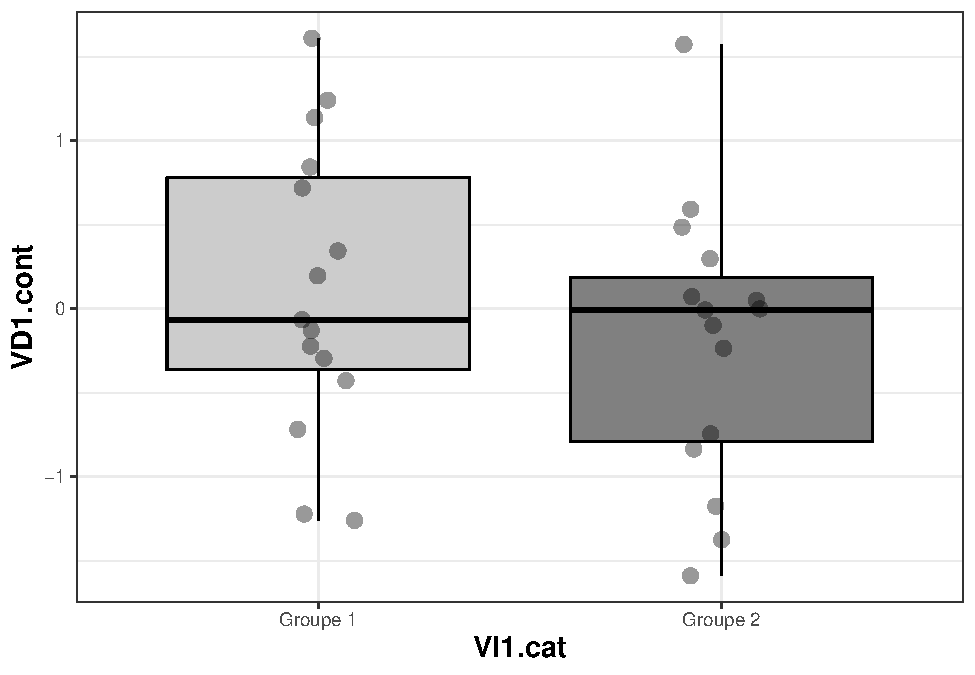
\includegraphics{Manuel_R_independant_files/figure-latex/unnamed-chunk-14-1.pdf}

\hypertarget{interpretation}{%
\subsubsection{Interpretation}\label{interpretation}}

{[}1{]} ``Les scores moyens du groupe 1 (M = 0.116, SD = 0.868, N = 15) et du groupe 2 (M = -0.2, SD = 0.831, N = 15) ne diffèrent pas statistiquement (t = 1.019, p = 0.317, d de cohen = 0.372)''

\hypertarget{anova-uxe0-un-facteur}{%
\subsection{ANOVA à un facteur}\label{anova-uxe0-un-facteur}}

\hypertarget{type-de-variables-1}{%
\subsubsection{Type de variables}\label{type-de-variables-1}}

\textbf{Variable Dépendante :} Numérique
\textbf{Variable Indépendante :} Catégorielle (3 catégories ou +)

\hypertarget{packages-nuxe9cessaires-1}{%
\subsubsection{Packages nécessaires}\label{packages-nuxe9cessaires-1}}

\begin{Shaded}
\begin{Highlighting}[]
\KeywordTok{library}\NormalTok{(ggplot2)}
\KeywordTok{library}\NormalTok{(GGally)}
\KeywordTok{library}\NormalTok{(dplyr)}
\KeywordTok{library}\NormalTok{(emmeans)}
\KeywordTok{library}\NormalTok{(car)}
\KeywordTok{library}\NormalTok{(forcats)}
\KeywordTok{library}\NormalTok{(rstatix)}
\KeywordTok{library}\NormalTok{(broom)}
\end{Highlighting}
\end{Shaded}

\hypertarget{donnuxe9es-ruxe9elles-1}{%
\subsubsection{Données réelles}\label{donnuxe9es-ruxe9elles-1}}

\begin{Shaded}
\begin{Highlighting}[]
\CommentTok{# choisissez la ligne appropriée au format de votre fichier de données. }

\CommentTok{# si vos données sont dans un fichier .txt}
\NormalTok{my_data.anova <-}\StringTok{ }\KeywordTok{read.delim}\NormalTok{(}\KeywordTok{file.choose}\NormalTok{())}

\CommentTok{# si vos données sont dans un fichier .csv}
\NormalTok{my_data.anova <-}\StringTok{ }\KeywordTok{read.csv}\NormalTok{(}\KeywordTok{file.choose}\NormalTok{())}

\CommentTok{# si vos données sont dans un fichier .xls / .xlsx}
\NormalTok{my_data.anova <-}\StringTok{ }\KeywordTok{read_excel}\NormalTok{(}\KeywordTok{file.choose}\NormalTok{())}

\CommentTok{# une fois vos données chargées, vous pouvez renommer vos noms de colonnes afin qu'ils correspondent à ceux utilisés dans le code ci-dessous}
\CommentTok{# Si vous ne souhaitez pas renommer vos noms de colonnes, sautez cette étape mais adaptez le code des parties suivantes en lui indiquant les noms de colonnes de vos données.}

\CommentTok{# On crée une nouvelle colonne pour votre variable dépendante continue (remplacez 'votre.nom.de.colonne' par le nom approprié)}
\NormalTok{my_data.anova}\OperatorTok{$}\NormalTok{VD1.cont <-}\StringTok{ }\NormalTok{my_data.anova}\OperatorTok{$}\StringTok{'votre.nom.de.colonne'}

\CommentTok{# On crée une nouvelle colonne pour votre variable indépendante catégorielle (remplacez 'votre.nom.de.colonne' par le nom approprié)}
\NormalTok{my_data.anova}\OperatorTok{$}\NormalTok{VI1.multicat <-}\StringTok{ }\NormalTok{my_data.anova}\OperatorTok{$}\StringTok{'votre.nom.de.colonne'}
\end{Highlighting}
\end{Shaded}

\hypertarget{donnuxe9es-fictives-1}{%
\subsubsection{Données fictives}\label{donnuxe9es-fictives-1}}

\begin{Shaded}
\begin{Highlighting}[]
\KeywordTok{set.seed}\NormalTok{(}\DecValTok{4321}\NormalTok{)}
\NormalTok{my_data.anova <-}\StringTok{ }\KeywordTok{data.frame}\NormalTok{(}
  \DataTypeTok{VD1.cont =} \KeywordTok{c}\NormalTok{(}\KeywordTok{rnorm}\NormalTok{(}\DecValTok{30}\NormalTok{)}\OperatorTok{-}\DecValTok{1}\NormalTok{, }\KeywordTok{rnorm}\NormalTok{(}\DecValTok{90}\NormalTok{)),}
  \DataTypeTok{VI1.multicat =} \KeywordTok{rep}\NormalTok{(}\KeywordTok{c}\NormalTok{(}\DecValTok{1}\NormalTok{, }\DecValTok{2}\NormalTok{, }\DecValTok{3}\NormalTok{, }\DecValTok{4}\NormalTok{), }\DataTypeTok{each =} \DecValTok{30}\NormalTok{))}

\CommentTok{# On renomme les catégories de VI1.cat pour que les résultats soient plus lisibles}
\NormalTok{ my_data.anova}\OperatorTok{$}\NormalTok{VI1.multicat <-}\StringTok{ }\KeywordTok{fct_recode}\NormalTok{(}\KeywordTok{factor}\NormalTok{(my_data.anova}\OperatorTok{$}\NormalTok{VI1.multicat), }
                                 \StringTok{"Groupe 1"}\NormalTok{ =}\StringTok{ "1"}\NormalTok{, }
                                 \StringTok{"Groupe 2"}\NormalTok{ =}\StringTok{ "2"}\NormalTok{, }
                                 \StringTok{"Groupe 3"}\NormalTok{ =}\StringTok{ "3"}\NormalTok{, }
                                 \StringTok{"Groupe 4"}\NormalTok{ =}\StringTok{ "4"}\NormalTok{) }
\end{Highlighting}
\end{Shaded}

\hypertarget{duxe9claration-du-type-de-variables}{%
\subsubsection{Déclaration du type de variables}\label{duxe9claration-du-type-de-variables}}

\begin{Shaded}
\begin{Highlighting}[]
\NormalTok{my_data.anova}\OperatorTok{$}\NormalTok{VD1.cont <-}\StringTok{ }\KeywordTok{as.numeric}\NormalTok{(}\KeywordTok{as.character}\NormalTok{(my_data.anova}\OperatorTok{$}\NormalTok{VD1.cont))}
\NormalTok{my_data.anova}\OperatorTok{$}\NormalTok{VI1.multicat <-}\StringTok{ }\KeywordTok{factor}\NormalTok{(my_data.anova}\OperatorTok{$}\NormalTok{VI1.multicat)}
\end{Highlighting}
\end{Shaded}

\hypertarget{inspection-des-donnuxe9es}{%
\subsubsection{Inspection des données}\label{inspection-des-donnuxe9es}}

\begin{Shaded}
\begin{Highlighting}[]
\CommentTok{## Les graphiques situés sur la diagonale représentent la distribution des variables}
\CommentTok{## Les graphiques (ou les valeurs de corrélation) situés au dessus et en dessous de la diagonale représentent les associations deux-à-deux}
\KeywordTok{ggpairs}\NormalTok{(my_data.anova,}
        \DataTypeTok{lower =} \KeywordTok{list}\NormalTok{(}\DataTypeTok{continuous =} \KeywordTok{wrap}\NormalTok{(}\StringTok{"smooth"}\NormalTok{, }\DataTypeTok{alpha =} \FloatTok{0.7}\NormalTok{), }\DataTypeTok{combo =} \StringTok{"box_no_facet"}\NormalTok{),}
        \DataTypeTok{upper =} \KeywordTok{list}\NormalTok{(}\DataTypeTok{combo =} \StringTok{"facetdensity"}\NormalTok{), }
        \DataTypeTok{mapping =} \KeywordTok{aes}\NormalTok{(}\DataTypeTok{alpha =} \FloatTok{0.8}\NormalTok{)) }\OperatorTok{+}\StringTok{ }\KeywordTok{theme_bw}\NormalTok{()}
\end{Highlighting}
\end{Shaded}

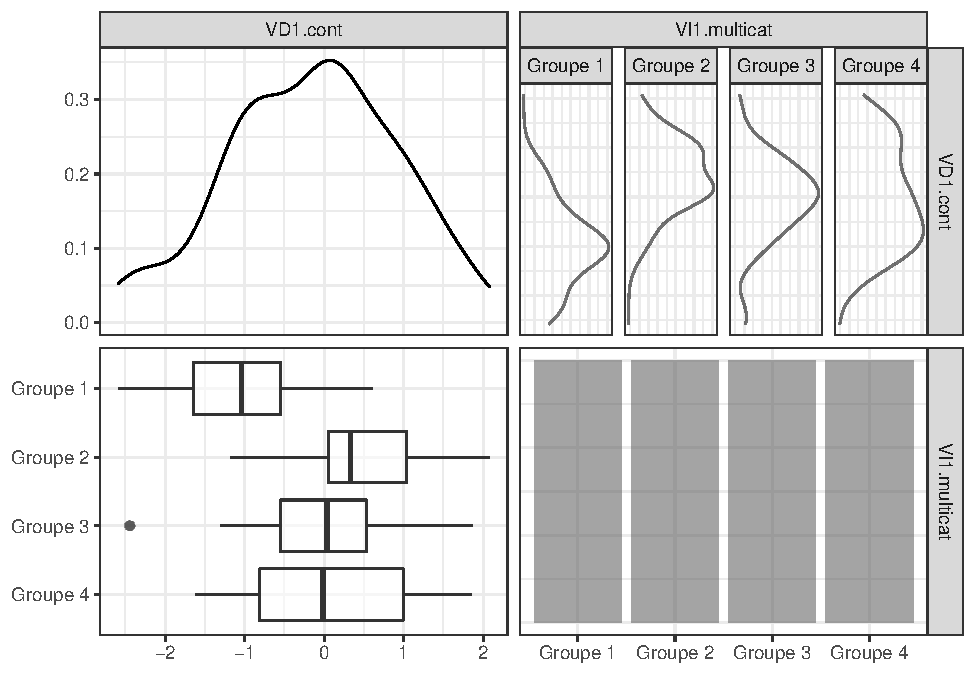
\includegraphics{Manuel_R_independant_files/figure-latex/unnamed-chunk-20-1.pdf}

\hypertarget{analyse-des-donnuxe9es-1}{%
\subsubsection{Analyse des données}\label{analyse-des-donnuxe9es-1}}

\begin{Shaded}
\begin{Highlighting}[]
\CommentTok{# calcul de l'ANOVA et stockage des résultats dans l’objet anova.test}
\NormalTok{anova.test <-}\StringTok{ }\KeywordTok{lm}\NormalTok{(}\DataTypeTok{formula =}\NormalTok{ VD1.cont }\OperatorTok{~}\StringTok{ }\NormalTok{VI1.multicat,}
                 \DataTypeTok{data =}\NormalTok{ my_data.anova)}

\CommentTok{# calcul des moyennes et écarts types pour chaque modalité de VI.multicat}
\NormalTok{description.anova <-}\StringTok{ }\NormalTok{my_data.anova }\OperatorTok\StringTok{ }
\StringTok{  }\KeywordTok{group_by}\NormalTok{(VI1.multicat) }\OperatorTok\StringTok{ }
\StringTok{  }\KeywordTok{summarise}\NormalTok{(}
    \DataTypeTok{Mean =} \KeywordTok{mean}\NormalTok{(VD1.cont),}
    \DataTypeTok{SD =} \KeywordTok{sd}\NormalTok{(VD1.cont),}
    \DataTypeTok{N =} \KeywordTok{n}\NormalTok{())}

\CommentTok{# calcul des tests post hoc (comparaison de moyennes deux à deux) ajustées par une procédure tukey.}
\NormalTok{posthoc.anova <-}\StringTok{ }\KeywordTok{emmeans}\NormalTok{(anova.test, pairwise }\OperatorTok{~}\StringTok{ }\NormalTok{VI1.multicat, }\DataTypeTok{adjust =} \StringTok{"tukey"}\NormalTok{)}

\CommentTok{# calcul de la taille d'effet de VI1.multicat sur VD1.cont (SMD / d de cohen)}
\NormalTok{cohensd.anova <-}\StringTok{ }\NormalTok{rstatix}\OperatorTok{::}\KeywordTok{cohens_d}\NormalTok{(}\DataTypeTok{data =}\NormalTok{ my_data.anova,}
                    \DataTypeTok{formula =}\NormalTok{ VD1.cont }\OperatorTok{~}\StringTok{ }\NormalTok{VI1.multicat, }
                    \DataTypeTok{var.equal =} \OtherTok{TRUE}\NormalTok{)}


\CommentTok{# obtention des différentes moyennes/écarts-types pour chaque groupe}
\NormalTok{description.anova}
\end{Highlighting}
\end{Shaded}

\begin{verbatim}
## # A tibble: 4 x 4
##   VI1.multicat    Mean    SD     N
##   <fct>          <dbl> <dbl> <int>
## 1 Groupe 1     -1.04   0.850    30
## 2 Groupe 2      0.464  0.758    30
## 3 Groupe 3     -0.0927 0.946    30
## 4 Groupe 4      0.0700 1.03     30
\end{verbatim}

\begin{Shaded}
\begin{Highlighting}[]
\CommentTok{# obtention des résultats de l'anova }
\KeywordTok{Anova}\NormalTok{(anova.test)}
\end{Highlighting}
\end{Shaded}

\begin{verbatim}
## Anova Table (Type II tests)
## 
## Response: VD1.cont
##              Sum Sq  Df F value    Pr(>F)    
## VI1.multicat 36.727   3  15.081 2.371e-08 ***
## Residuals    94.169 116                      
## ---
## Signif. codes:  0 '***' 0.001 '**' 0.01 '*' 0.05 '.' 0.1 ' ' 1
\end{verbatim}

\begin{Shaded}
\begin{Highlighting}[]
\CommentTok{# obtention des tests post hoc }
\NormalTok{posthoc.anova}
\end{Highlighting}
\end{Shaded}

\begin{verbatim}
## $emmeans
##  VI1.multicat  emmean    SE  df lower.CL upper.CL
##  Groupe 1     -1.0418 0.164 116  -1.4581   -0.626
##  Groupe 2      0.4642 0.164 116   0.0479    0.880
##  Groupe 3     -0.0927 0.164 116  -0.5089    0.324
##  Groupe 4      0.0700 0.164 116  -0.3462    0.486
## 
## Confidence level used: 0.95 
## Conf-level adjustment: sidak method for 4 estimates 
## 
## $contrasts
##  contrast            estimate    SE  df t.ratio p.value
##  Groupe 1 - Groupe 2   -1.506 0.233 116 -6.474  <.0001 
##  Groupe 1 - Groupe 3   -0.949 0.233 116 -4.080  0.0005 
##  Groupe 1 - Groupe 4   -1.112 0.233 116 -4.779  <.0001 
##  Groupe 2 - Groupe 3    0.557 0.233 116  2.394  0.0840 
##  Groupe 2 - Groupe 4    0.394 0.233 116  1.694  0.3313 
##  Groupe 3 - Groupe 4   -0.163 0.233 116 -0.699  0.8972 
## 
## P value adjustment: tukey method for comparing a family of 4 estimates
\end{verbatim}

\begin{Shaded}
\begin{Highlighting}[]
\CommentTok{# obtention des tailles d'effet }
\NormalTok{cohensd.anova}
\end{Highlighting}
\end{Shaded}

\begin{verbatim}
## # A tibble: 6 x 7
##   .y.      group1   group2   effsize    n1    n2 magnitude 
## * <chr>    <chr>    <chr>      <dbl> <int> <int> <ord>     
## 1 VD1.cont Groupe 1 Groupe 2  -1.87     30    30 large     
## 2 VD1.cont Groupe 1 Groupe 3  -1.06     30    30 large     
## 3 VD1.cont Groupe 1 Groupe 4  -1.18     30    30 large     
## 4 VD1.cont Groupe 2 Groupe 3   0.650    30    30 moderate  
## 5 VD1.cont Groupe 2 Groupe 4   0.437    30    30 small     
## 6 VD1.cont Groupe 3 Groupe 4  -0.165    30    30 negligible
\end{verbatim}

\hypertarget{graphique-1}{%
\subsubsection{Graphique}\label{graphique-1}}

\begin{Shaded}
\begin{Highlighting}[]
\KeywordTok{ggplot}\NormalTok{(my_data.anova, }\KeywordTok{aes}\NormalTok{(}\DataTypeTok{x =}\NormalTok{ VI1.multicat, }\DataTypeTok{y =}\NormalTok{ VD1.cont, }\DataTypeTok{fill =}\NormalTok{ VI1.multicat)) }\OperatorTok{+}
\StringTok{  }\KeywordTok{geom_boxplot}\NormalTok{(}\DataTypeTok{color=}\StringTok{"black"}\NormalTok{, }\DataTypeTok{outlier.color=}\StringTok{"red"}\NormalTok{) }\OperatorTok{+}\StringTok{ }
\StringTok{  }\KeywordTok{geom_jitter}\NormalTok{(}\DataTypeTok{size =} \DecValTok{3}\NormalTok{, }\DataTypeTok{alpha=}\FloatTok{0.4}\NormalTok{, }\DataTypeTok{width=}\FloatTok{0.1}\NormalTok{) }\OperatorTok{+}\StringTok{ }
\StringTok{  }\KeywordTok{ylab}\NormalTok{(}\StringTok{"VD1.cont"}\NormalTok{) }\OperatorTok{+}\StringTok{ }\KeywordTok{xlab}\NormalTok{(}\StringTok{"VI1.cat"}\NormalTok{) }\OperatorTok{+}\StringTok{ }
\StringTok{  }\KeywordTok{theme_bw}\NormalTok{() }\OperatorTok{+}\StringTok{ }
\StringTok{  }\KeywordTok{theme}\NormalTok{(}\DataTypeTok{axis.title.y =} \KeywordTok{element_text}\NormalTok{(}\DataTypeTok{size =} \DecValTok{14}\NormalTok{, }\DataTypeTok{hjust =} \FloatTok{0.5}\NormalTok{, }\DataTypeTok{face=}\StringTok{"bold"}\NormalTok{), }
        \DataTypeTok{axis.title.x =} \KeywordTok{element_text}\NormalTok{(}\DataTypeTok{face=}\StringTok{"bold"}\NormalTok{, }\DataTypeTok{size =} \DecValTok{14}\NormalTok{, }\DataTypeTok{hjust =} \FloatTok{0.5}\NormalTok{)) }\OperatorTok{+}
\StringTok{  }\KeywordTok{scale_fill_grey}\NormalTok{(}\DataTypeTok{start =} \FloatTok{0.9}\NormalTok{, }\DataTypeTok{end =} \FloatTok{0.5}\NormalTok{) }\OperatorTok{+}
\StringTok{  }\KeywordTok{guides}\NormalTok{(}\DataTypeTok{fill =} \OtherTok{FALSE}\NormalTok{)}
\end{Highlighting}
\end{Shaded}

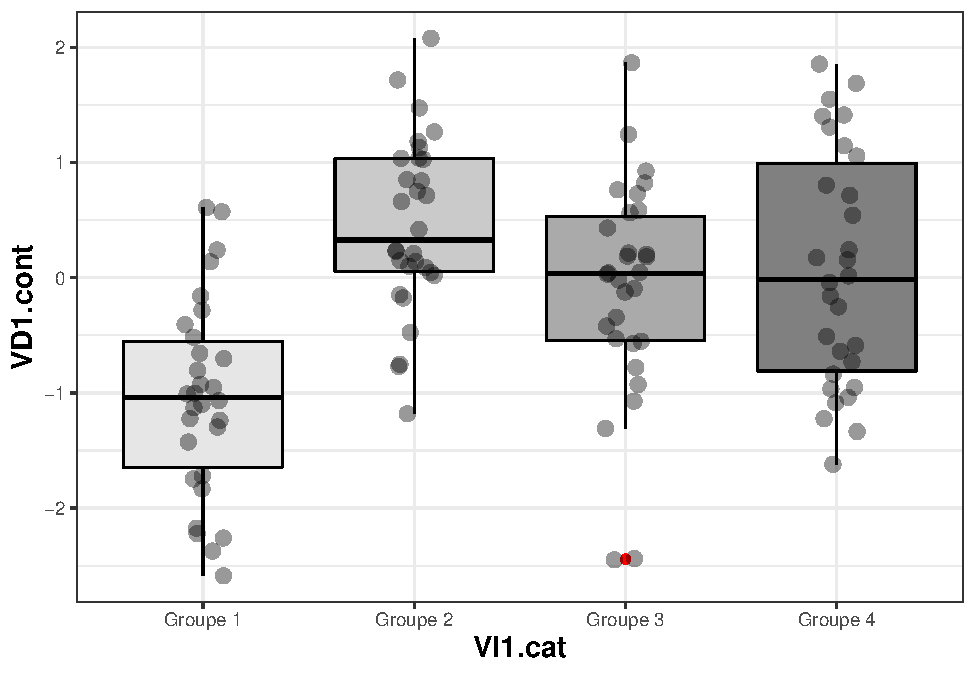
\includegraphics{Manuel_R_independant_files/figure-latex/unnamed-chunk-22-1.pdf}

\hypertarget{interpretation-1}{%
\subsubsection{Interpretation}\label{interpretation-1}}

{[}1{]} ``L'effet principal de VI1.multicat est significatif (F = 15.081, p = 2e-08). Les scores moyens du groupe 1 (M = -1.042, SD = 0.85, N = 30) sont significativement plus faibles que les scores moyens de 3 autres groupes (toutes les valeurs p ajustées \textless{} 0.00048, d de cohen \textgreater{} 1.055). Aucune autre différence n'atteint la significativité (toutes les valeurs p ajustées \textgreater{} 0.084, d de cohen \textless{} 0.65)''

\hypertarget{corruxe9lation}{%
\subsection{Corrélation}\label{corruxe9lation}}

\hypertarget{type-de-variables-2}{%
\subsubsection{Type de variables}\label{type-de-variables-2}}

\textbf{Variable Dépendante :} Numérique
\textbf{Variable Indépendante :} Numérique

\hypertarget{packages-nuxe9cessaires-2}{%
\subsubsection{Packages nécessaires}\label{packages-nuxe9cessaires-2}}

\begin{Shaded}
\begin{Highlighting}[]
\KeywordTok{library}\NormalTok{(ggplot2)}
\KeywordTok{library}\NormalTok{(GGally)}
\KeywordTok{library}\NormalTok{(rstatix)}
\KeywordTok{library}\NormalTok{(dplyr)}
\end{Highlighting}
\end{Shaded}

\hypertarget{donnuxe9es-ruxe9elles-2}{%
\subsubsection{Données réelles}\label{donnuxe9es-ruxe9elles-2}}

\begin{Shaded}
\begin{Highlighting}[]
\CommentTok{# choisissez la ligne appropriée au format de votre fichier de données. }

\CommentTok{# si vos données sont dans un fichier .txt}
\NormalTok{my_data.correlation <-}\StringTok{ }\KeywordTok{read.delim}\NormalTok{(}\KeywordTok{file.choose}\NormalTok{())}

\CommentTok{# si vos données sont dans un fichier .csv}
\NormalTok{my_data.correlation <-}\StringTok{ }\KeywordTok{read.csv}\NormalTok{(}\KeywordTok{file.choose}\NormalTok{())}

\CommentTok{# si vos données sont dans un fichier .xls / .xlsx}
\NormalTok{my_data.correlation <-}\StringTok{ }\KeywordTok{read_excel}\NormalTok{(}\KeywordTok{file.choose}\NormalTok{())}

\CommentTok{# une fois vos données chargées, vous pouvez renommer vos noms de colonnes afin qu'ils correspondent à ceux utilisés dans le code ci-dessous}
\CommentTok{# Si vous ne souhaitez pas renommer vos noms de colonnes, sautez cette étape mais adaptez le code des parties suivantes en lui indiquant les noms de colonnes de vos données.}

\CommentTok{# On crée une nouvelle colonne pour votre variable dépendante continue (remplacez 'votre.nom.de.colonne' par le nom approprié)}
\NormalTok{my_data.correlation}\OperatorTok{$}\NormalTok{VD1.cont <-}\StringTok{ }\NormalTok{my_data.correlation}\OperatorTok{$}\StringTok{'votre.nom.de.colonne'}

\CommentTok{# On crée une nouvelle colonne pour votre variable indépendante continue (remplacez 'votre.nom.de.colonne' par le nom approprié)}
\NormalTok{my_data.correlation}\OperatorTok{$}\NormalTok{VI1.cont <-}\StringTok{ }\NormalTok{my_data.correlation}\OperatorTok{$}\StringTok{'votre.nom.de.colonne'}
\end{Highlighting}
\end{Shaded}

\hypertarget{donnuxe9es-fictives-2}{%
\subsubsection{Données fictives}\label{donnuxe9es-fictives-2}}

\begin{Shaded}
\begin{Highlighting}[]
\KeywordTok{set.seed}\NormalTok{(}\DecValTok{4321}\NormalTok{)}
\NormalTok{cor <-}\StringTok{ }\KeywordTok{rnorm}\NormalTok{(}\DecValTok{130}\NormalTok{)}
\NormalTok{my_data.correlation <-}\StringTok{ }\KeywordTok{data.frame}\NormalTok{(}
  \DataTypeTok{VD1.cont =} \KeywordTok{rnorm}\NormalTok{(}\DecValTok{130}\NormalTok{) }\OperatorTok{+}\StringTok{ }\FloatTok{0.5}\OperatorTok{*}\NormalTok{cor,}
  \DataTypeTok{VI1.cont =} \KeywordTok{rnorm}\NormalTok{(}\DecValTok{130}\NormalTok{) }\OperatorTok{+}\StringTok{ }\FloatTok{0.5}\OperatorTok{*}\NormalTok{cor)}
\end{Highlighting}
\end{Shaded}

\hypertarget{duxe9claration-du-type-de-variables-1}{%
\subsubsection{Déclaration du type de variables}\label{duxe9claration-du-type-de-variables-1}}

\begin{Shaded}
\begin{Highlighting}[]
\NormalTok{my_data.correlation}\OperatorTok{$}\NormalTok{VD1.cont <-}\StringTok{ }\KeywordTok{as.numeric}\NormalTok{(}\KeywordTok{as.character}\NormalTok{(my_data.correlation}\OperatorTok{$}\NormalTok{VD1.cont))}
\NormalTok{my_data.correlation}\OperatorTok{$}\NormalTok{VI1.cont <-}\StringTok{ }\KeywordTok{as.numeric}\NormalTok{(}\KeywordTok{as.character}\NormalTok{(my_data.correlation}\OperatorTok{$}\NormalTok{VI1.cont))}
\end{Highlighting}
\end{Shaded}

\hypertarget{inspection-des-donnuxe9es-1}{%
\subsubsection{Inspection des données}\label{inspection-des-donnuxe9es-1}}

\begin{Shaded}
\begin{Highlighting}[]
\CommentTok{## Les graphiques situés sur la diagonale représentent la distribution des variables}
\CommentTok{## Les graphiques (ou les valeurs de corrélation) situés au dessus et en dessous de la diagonale représentent les associations deux-à-deux}
\KeywordTok{ggpairs}\NormalTok{(my_data.correlation,}
        \DataTypeTok{lower =} \KeywordTok{list}\NormalTok{(}\DataTypeTok{continuous =} \KeywordTok{wrap}\NormalTok{(}\StringTok{"smooth"}\NormalTok{, }\DataTypeTok{alpha =} \FloatTok{0.7}\NormalTok{), }\DataTypeTok{combo =} \StringTok{"box_no_facet"}\NormalTok{),}
        \DataTypeTok{upper =} \KeywordTok{list}\NormalTok{(}\DataTypeTok{combo =} \StringTok{"facetdensity"}\NormalTok{, }\DataTypeTok{discrete =} \StringTok{"facetbar"}\NormalTok{), }
        \DataTypeTok{mapping =} \KeywordTok{aes}\NormalTok{(}\DataTypeTok{alpha =} \FloatTok{0.8}\NormalTok{)) }\OperatorTok{+}\StringTok{ }\KeywordTok{theme_bw}\NormalTok{()}
\end{Highlighting}
\end{Shaded}

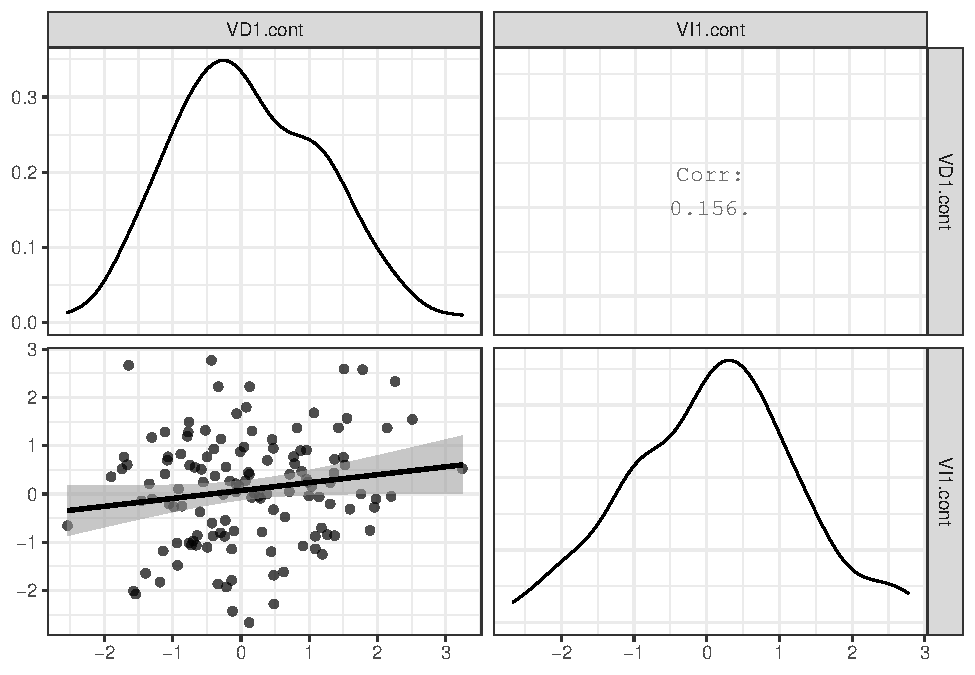
\includegraphics{Manuel_R_independant_files/figure-latex/unnamed-chunk-28-1.pdf}

\hypertarget{analyse-des-donnuxe9es-2}{%
\subsubsection{Analyse des données}\label{analyse-des-donnuxe9es-2}}

\begin{Shaded}
\begin{Highlighting}[]
\CommentTok{# calcul de la corrélation et stockage des résultats dans l’objet correlation.test}
\NormalTok{correlation.test <-}\StringTok{ }\KeywordTok{cor.test}\NormalTok{(}\DataTypeTok{formula =} \OperatorTok{~}\StringTok{ }\NormalTok{VD1.cont }\OperatorTok{+}\StringTok{ }\NormalTok{VI1.cont, }
                 \DataTypeTok{data =}\NormalTok{ my_data.correlation,}
                 \DataTypeTok{method =} \StringTok{"pearson"}\NormalTok{)}

\CommentTok{# obtention des résultats de la correlation }
\NormalTok{correlation.test}
\end{Highlighting}
\end{Shaded}

\begin{verbatim}
## 
## 	Pearson's product-moment correlation
## 
## data:  VD1.cont and VI1.cont
## t = 1.7884, df = 128, p-value = 0.07607
## alternative hypothesis: true correlation is not equal to 0
## 95 percent confidence interval:
##  -0.01649018  0.31972942
## sample estimates:
##       cor 
## 0.1561393
\end{verbatim}

\hypertarget{graphique-2}
\KeywordTok{ggplot}\NormalTok{(my_data.correlation, }\KeywordTok{aes}\NormalTok{(}\DataTypeTok{x =}\NormalTok{ VI1.cont, }\DataTypeTok{y =}\NormalTok{ VD1.cont)) }\OperatorTok{+}
\StringTok{  }\KeywordTok{geom_point}\NormalTok{(}\DataTypeTok{size =} \DecValTok{3}\NormalTok{, }\DataTypeTok{alpha =} \FloatTok{0.4}\NormalTok{) }\OperatorTok{+}\StringTok{ }
\StringTok{  }\KeywordTok{geom_smooth}\NormalTok{(}\DataTypeTok{formula =}\NormalTok{ y }\OperatorTok{~}\StringTok{ }\NormalTok{x, }\DataTypeTok{method =} \StringTok{"lm"}\NormalTok{) }\OperatorTok{+}
\StringTok{  }\KeywordTok{ylab}\NormalTok{(}\StringTok{"VD1.cont"}\NormalTok{) }\OperatorTok{+}\StringTok{ }\KeywordTok{xlab}\NormalTok{(}\StringTok{"VI1.cont"}\NormalTok{) }\OperatorTok{+}\StringTok{ }
\StringTok{  }\KeywordTok{theme_bw}\NormalTok{() }\OperatorTok{+}\StringTok{ }
\StringTok{  }\KeywordTok{theme}\NormalTok{(}\DataTypeTok{axis.title.y =} \KeywordTok{element_text}\NormalTok{(}\DataTypeTok{size =} \DecValTok{14}\NormalTok{, }\DataTypeTok{hjust =} \FloatTok{0.5}\NormalTok{, }\DataTypeTok{face =} \StringTok{"bold"}\NormalTok{), }
        \DataTypeTok{axis.title.x =} \KeywordTok{element_text}\NormalTok{(}\DataTypeTok{face =} \StringTok{"bold"}\NormalTok{, }\DataTypeTok{size =} \DecValTok{14}\NormalTok{, }\DataTypeTok{hjust =} \FloatTok{0.5}\NormalTok{))}
\end{Highlighting}
\end{Shaded}

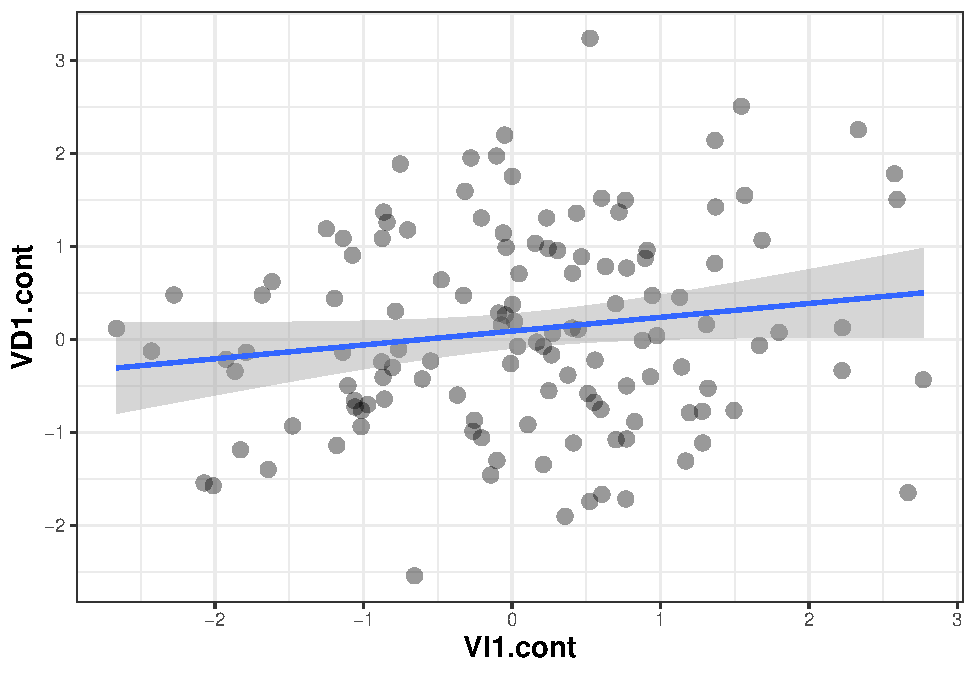
\includegraphics{Manuel_R_independant_files/figure-latex/unnamed-chunk-30-1.pdf}

\hypertarget{interpretation-2}{%
\subsubsection{Interpretation}\label{interpretation-2}}

{[}1{]} ``La correlation entre les variables VD1.cont et VI.cont est faible et la valeur p de cette association est marginalement significative (r = 0.156, 95\% IC = {[}-0.016, 0.32{]}, p = 0.076)''

\hypertarget{anova-multifactorielle}{%
\subsection{ANOVA multifactorielle}\label{anova-multifactorielle}}

\hypertarget{type-de-variables-3}{%
\subsubsection{Type de variables}\label{type-de-variables-3}}

\textbf{Variable Dépendante :} Numérique
\textbf{Variables Indépendantes :} Catégorielles (2 catégories ou +)

\hypertarget{packages-nuxe9cessaires-3}{%
\subsubsection{Packages nécessaires}\label{packages-nuxe9cessaires-3}}

\begin{Shaded}
\begin{Highlighting}[]
\KeywordTok{library}\NormalTok{(ggplot2)}
\KeywordTok{library}\NormalTok{(GGally)}
\KeywordTok{library}\NormalTok{(dplyr)}
\KeywordTok{library}\NormalTok{(emmeans)}
\KeywordTok{library}\NormalTok{(car)}
\KeywordTok{library}\NormalTok{(forcats)}
\KeywordTok{library}\NormalTok{(rstatix)}
\end{Highlighting}
\end{Shaded}

\hypertarget{donnuxe9es-ruxe9elles-3}{%
\subsubsection{Données réelles}\label{donnuxe9es-ruxe9elles-3}}

\begin{Shaded}
\begin{Highlighting}[]
\CommentTok{# choisissez la ligne appropriée au format de votre fichier de données. }

\CommentTok{# si vos données sont dans un fichier .txt}
\NormalTok{my_data.anovafact <-}\StringTok{ }\KeywordTok{read.delim}\NormalTok{(}\KeywordTok{file.choose}\NormalTok{())}

\CommentTok{# si vos données sont dans un fichier .csv}
\NormalTok{my_data.anovafact <-}\StringTok{ }\KeywordTok{read.csv}\NormalTok{(}\KeywordTok{file.choose}\NormalTok{())}

\CommentTok{# si vos données sont dans un fichier .xls / .xlsx}
\NormalTok{my_data.anovafact <-}\StringTok{ }\KeywordTok{read_excel}\NormalTok{(}\KeywordTok{file.choose}\NormalTok{())}

\CommentTok{# une fois vos données chargées, vous pouvez renommer vos noms de colonnes afin qu'ils correspondent à ceux utilisés dans le code ci-dessous}
\CommentTok{# Si vous ne souhaitez pas renommer vos noms de colonnes, sautez cette étape mais adaptez le code des parties suivantes en lui indiquant les noms de colonnes de vos données.}

\CommentTok{# On crée une nouvelle colonne pour votre variable dépendante continue (remplacez 'votre.nom.de.colonne' par le nom approprié)}
\NormalTok{my_data.anovafact}\OperatorTok{$}\NormalTok{VD1.cont <-}\StringTok{ }\NormalTok{my_data.anovafact}\OperatorTok{$}\StringTok{'votre.nom.de.colonne'}

\CommentTok{# On crée une nouvelle colonne pour vos variables indépendantes catégorielles (remplacez 'votre.nom.de.colonne' par les noms appropriés)}
\NormalTok{my_data.anovafact}\OperatorTok{$}\NormalTok{VI1.cat <-}\StringTok{ }\NormalTok{my_data.anovafact}\OperatorTok{$}\StringTok{'votre.nom.de.colonne'}
\NormalTok{my_data.anovafact}\OperatorTok{$}\NormalTok{VI2.cat <-}\StringTok{ }\NormalTok{my_data.anovafact}\OperatorTok{$}\StringTok{'votre.nom.de.colonne'}
\end{Highlighting}
\end{Shaded}

\hypertarget{donnuxe9es-fictives-3}{%
\subsubsection{Données fictives}\label{donnuxe9es-fictives-3}}

\begin{Shaded}
\begin{Highlighting}[]
\KeywordTok{set.seed}\NormalTok{(}\DecValTok{4321}\NormalTok{)}
\NormalTok{my_data.anovafact <-}\StringTok{ }\KeywordTok{data.frame}\NormalTok{(}
  \DataTypeTok{VD1.cont =} \KeywordTok{c}\NormalTok{(}\KeywordTok{rnorm}\NormalTok{(}\DecValTok{20}\NormalTok{)}\OperatorTok{-}\FloatTok{0.5}\NormalTok{, }\KeywordTok{rnorm}\NormalTok{(}\DecValTok{20}\NormalTok{), }\KeywordTok{rnorm}\NormalTok{(}\DecValTok{20}\NormalTok{)}\OperatorTok{+}\FloatTok{0.5}\NormalTok{, }\KeywordTok{rnorm}\NormalTok{(}\DecValTok{20}\NormalTok{)),}
  \DataTypeTok{VI1.cat =} \KeywordTok{rep}\NormalTok{(}\KeywordTok{c}\NormalTok{(}\DecValTok{1}\NormalTok{, }\DecValTok{2}\NormalTok{), }\DataTypeTok{each =} \DecValTok{40}\NormalTok{),}
  \DataTypeTok{VI2.cat =} \KeywordTok{rep}\NormalTok{(}\KeywordTok{c}\NormalTok{(}\DecValTok{1}\NormalTok{, }\DecValTok{2}\NormalTok{, }\DecValTok{1}\NormalTok{, }\DecValTok{2}\NormalTok{), }\DataTypeTok{each =} \DecValTok{20}\NormalTok{))}

\CommentTok{# On renomme les catégories de VI1.cat et VI2.cat pour que les résultats soient plus lisibles}
\NormalTok{my_data.anovafact}\OperatorTok{$}\NormalTok{VI1.cat <-}\StringTok{ }\KeywordTok{fct_recode}\NormalTok{(}\KeywordTok{factor}\NormalTok{(my_data.anovafact}\OperatorTok{$}\NormalTok{VI1.cat), }
                                        \StringTok{"Groupe 1"}\NormalTok{ =}\StringTok{ "1"}\NormalTok{, }
                                        \StringTok{"Groupe 2"}\NormalTok{ =}\StringTok{ "2"}\NormalTok{) }

\NormalTok{my_data.anovafact}\OperatorTok{$}\NormalTok{VI2.cat <-}\StringTok{ }\KeywordTok{fct_recode}\NormalTok{(}\KeywordTok{factor}\NormalTok{(my_data.anovafact}\OperatorTok{$}\NormalTok{VI2.cat), }
                                        \StringTok{"Modalite 1"}\NormalTok{ =}\StringTok{ "1"}\NormalTok{, }
                                        \StringTok{"Modalite 2"}\NormalTok{ =}\StringTok{ "2"}\NormalTok{) }
\end{Highlighting}
\end{Shaded}

\hypertarget{duxe9claration-du-type-de-variables-2}{%
\subsubsection{Déclaration du type de variables}\label{duxe9claration-du-type-de-variables-2}}

\begin{Shaded}
\begin{Highlighting}[]
\NormalTok{my_data.anovafact}\OperatorTok{$}\NormalTok{VD1.cont <-}\StringTok{ }\KeywordTok{as.numeric}\NormalTok{(}\KeywordTok{as.character}\NormalTok{(my_data.anovafact}\OperatorTok{$}\NormalTok{VD1.cont))}
\NormalTok{my_data.anovafact}\OperatorTok{$}\NormalTok{VI1.cat <-}\StringTok{ }\KeywordTok{factor}\NormalTok{(my_data.anovafact}\OperatorTok{$}\NormalTok{VI1.cat)}
\NormalTok{my_data.anovafact}\OperatorTok{$}\NormalTok{VI2.cat <-}\StringTok{ }\KeywordTok{factor}\NormalTok{(my_data.anovafact}\OperatorTok{$}\NormalTok{VI2.cat)}
\end{Highlighting}
\end{Shaded}

\hypertarget{inspection-des-donnuxe9es-2}{%
\subsubsection{Inspection des données}\label{inspection-des-donnuxe9es-2}}

\begin{Shaded}
\begin{Highlighting}[]
\CommentTok{## Les graphiques situés sur la diagonale représentent la distribution des variables}
\CommentTok{## Les graphiques (ou les valeurs de corrélation) situés au dessus et en dessous de la diagonale représentent l'association entre les différentes variables}
\KeywordTok{ggpairs}\NormalTok{(my_data.anovafact,}
        \DataTypeTok{lower =} \KeywordTok{list}\NormalTok{(}\DataTypeTok{continuous =} \KeywordTok{wrap}\NormalTok{(}\StringTok{"smooth"}\NormalTok{, }\DataTypeTok{alpha =} \FloatTok{0.7}\NormalTok{), }\DataTypeTok{combo =} \StringTok{"box_no_facet"}\NormalTok{),}
        \DataTypeTok{upper =} \KeywordTok{list}\NormalTok{(}\DataTypeTok{combo =} \StringTok{"facetdensity"}\NormalTok{, }\DataTypeTok{discrete =} \StringTok{"facetbar"}\NormalTok{), }
        \DataTypeTok{mapping =} \KeywordTok{aes}\NormalTok{(}\DataTypeTok{alpha =} \FloatTok{0.8}\NormalTok{)) }\OperatorTok{+}\StringTok{ }\KeywordTok{theme_bw}\NormalTok{()}
\end{Highlighting}
\end{Shaded}

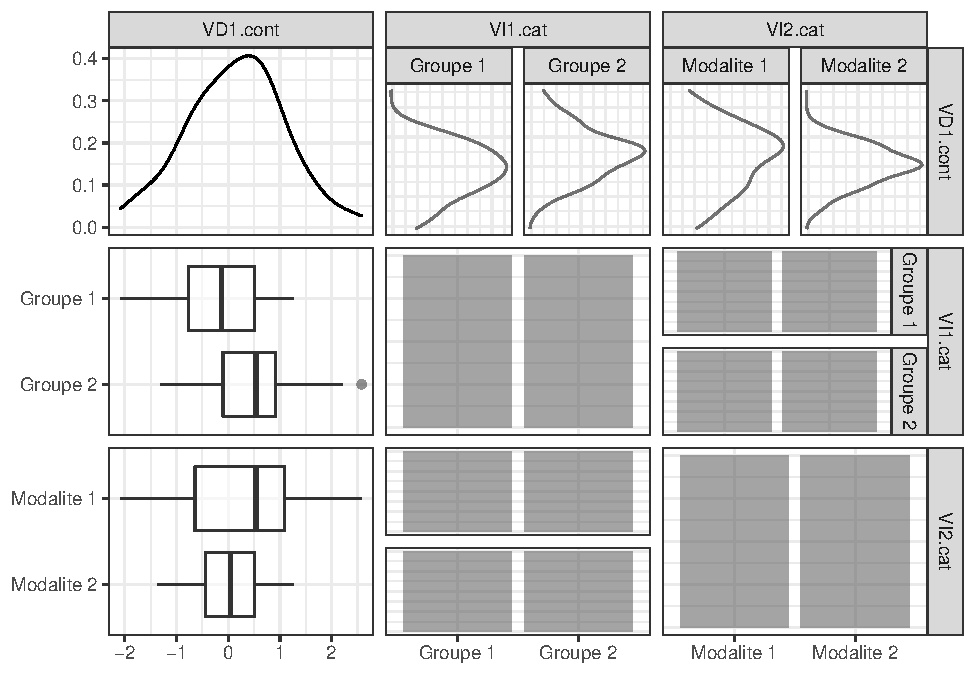
\includegraphics{Manuel_R_independant_files/figure-latex/unnamed-chunk-36-1.pdf}

\hypertarget{analyse-des-donnuxe9es-3}{%
\subsubsection{Analyse des données}\label{analyse-des-donnuxe9es-3}}

\begin{Shaded}
\begin{Highlighting}[]
\CommentTok{# calcul de l'ANOVA et stockage des résultats dans l’objet anovafact.test}
\NormalTok{anovafact.test <-}\StringTok{ }\KeywordTok{lm}\NormalTok{(}\DataTypeTok{formula =}\NormalTok{ VD1.cont }\OperatorTok{~}\StringTok{ }\NormalTok{VI1.cat}\OperatorTok{*}\NormalTok{VI2.cat,}
                     \DataTypeTok{contrasts =} \KeywordTok{list}\NormalTok{(}
                       \DataTypeTok{VI1.cat=}\StringTok{"contr.sum"}\NormalTok{,}
                       \DataTypeTok{VI2.cat=}\StringTok{"contr.sum"}\NormalTok{),}
                     \DataTypeTok{data =}\NormalTok{ my_data.anovafact)}

\CommentTok{# calcul des moyennes et écarts types pour lchaque modalité de VI.multicat}
\NormalTok{description.anovafact <-}\StringTok{ }\NormalTok{my_data.anovafact }\OperatorTok\StringTok{ }
\StringTok{  }\KeywordTok{group_by}\NormalTok{(VI1.cat, VI2.cat) }\OperatorTok\StringTok{ }
\StringTok{  }\KeywordTok{summarise}\NormalTok{(}
    \DataTypeTok{Mean=}\KeywordTok{mean}\NormalTok{(VD1.cont),}
    \DataTypeTok{SD=}\KeywordTok{sd}\NormalTok{(VD1.cont),}
    \DataTypeTok{N=}\KeywordTok{n}\NormalTok{())}

\CommentTok{# calcul des tests post hoc (comparaison de moyennes deux à deux) sans ajuster la valeur p}
\NormalTok{posthoc.anovafact <-}\StringTok{ }\KeywordTok{emmeans}\NormalTok{(anovafact.test, consec }\OperatorTok{~}\StringTok{ }\NormalTok{VI1.cat }\OperatorTok{|}\StringTok{ }\NormalTok{VI2.cat, }\DataTypeTok{adjust=}\StringTok{"none"}\NormalTok{)}

\CommentTok{# calcul de la taille d'effet de VI1.cat et VI2.cat sur VD1.cont (SMD / d de cohen)}
\NormalTok{my_data.anovafact}\OperatorTok{$}\NormalTok{VI.comb <-}\StringTok{ }\KeywordTok{interaction}\NormalTok{(my_data.anovafact}\OperatorTok{$}\NormalTok{VI1.cat, my_data.anovafact}\OperatorTok{$}\NormalTok{VI2.cat)}
\NormalTok{cohensd.anovafact <-}\StringTok{ }\NormalTok{rstatix}\OperatorTok{::}\KeywordTok{cohens_d}\NormalTok{(}\DataTypeTok{data =}\NormalTok{ my_data.anovafact,}
                              \DataTypeTok{formula =}\NormalTok{ VD1.cont }\OperatorTok{~}\StringTok{ }\NormalTok{VI.comb, }
                              \DataTypeTok{var.equal =} \OtherTok{TRUE}\NormalTok{)}

\CommentTok{# obtention des différentes moyennes/écarts-types }
\NormalTok{description.anovafact}
\end{Highlighting}
\end{Shaded}

\begin{verbatim}
## # A tibble: 4 x 5
## # Groups:   VI1.cat [2]
##   VI1.cat  VI2.cat       Mean    SD     N
##   <fct>    <fct>        <dbl> <dbl> <int>
## 1 Groupe 1 Modalite 1 -0.506  0.965    20
## 2 Groupe 1 Modalite 2  0.125  0.670    20
## 3 Groupe 2 Modalite 1  1.01   0.806    20
## 4 Groupe 2 Modalite 2 -0.0407 0.618    20
\end{verbatim}

\begin{Shaded}
\begin{Highlighting}[]
\CommentTok{# obtention des résultats de l'anova }
\KeywordTok{Anova}\NormalTok{(anovafact.test, }\DataTypeTok{type =} \DecValTok{3}\NormalTok{)}
\end{Highlighting}
\end{Shaded}

\begin{verbatim}
## Anova Table (Type III tests)
## 
## Response: VD1.cont
##                 Sum Sq Df F value    Pr(>F)    
## (Intercept)      1.757  1  2.9149 0.0918473 .  
## VI1.cat          9.170  1 15.2159 0.0002055 ***
## VI2.cat          0.898  1  1.4897 0.2260313    
## VI1.cat:VI2.cat 14.215  1 23.5880 6.245e-06 ***
## Residuals       45.802 76                      
## ---
## Signif. codes:  0 '***' 0.001 '**' 0.01 '*' 0.05 '.' 0.1 ' ' 1
\end{verbatim}

\begin{Shaded}
\begin{Highlighting}[]
\CommentTok{# obtention des tests post hoc }
\NormalTok{posthoc.anovafact}
\end{Highlighting}
\end{Shaded}

\begin{verbatim}
## $emmeans
## VI2.cat = Modalite 1:
##  VI1.cat   emmean    SE df lower.CL upper.CL
##  Groupe 1 -0.5060 0.174 76   -0.852   -0.160
##  Groupe 2  1.0142 0.174 76    0.668    1.360
## 
## VI2.cat = Modalite 2:
##  VI1.cat   emmean    SE df lower.CL upper.CL
##  Groupe 1  0.1252 0.174 76   -0.221    0.471
##  Groupe 2 -0.0407 0.174 76   -0.386    0.305
## 
## Confidence level used: 0.95 
## 
## $contrasts
## VI2.cat = Modalite 1:
##  contrast            estimate    SE df t.ratio p.value
##  Groupe 2 - Groupe 1    1.520 0.245 76  6.192  <.0001 
## 
## VI2.cat = Modalite 2:
##  contrast            estimate    SE df t.ratio p.value
##  Groupe 2 - Groupe 1   -0.166 0.245 76 -0.676  0.5011
\end{verbatim}

\begin{Shaded}
\begin{Highlighting}[]
\CommentTok{# obtention de la taille d'effet }
\NormalTok{cohensd.anovafact}
\end{Highlighting}
\end{Shaded}

\begin{verbatim}
## # A tibble: 6 x 7
##   .y.      group1              group2              effsize    n1    n2 magnitude
## * <chr>    <chr>               <chr>                 <dbl> <int> <int> <ord>    
## 1 VD1.cont Groupe 1.Modalite 1 Groupe 2.Modalite 1  -1.71     20    20 large    
## 2 VD1.cont Groupe 1.Modalite 1 Groupe 1.Modalite 2  -0.760    20    20 moderate 
## 3 VD1.cont Groupe 1.Modalite 1 Groupe 2.Modalite 2  -0.574    20    20 moderate 
## 4 VD1.cont Groupe 2.Modalite 1 Groupe 1.Modalite 2   1.20     20    20 large    
## 5 VD1.cont Groupe 2.Modalite 1 Groupe 2.Modalite 2   1.47     20    20 large    
## 6 VD1.cont Groupe 1.Modalite 2 Groupe 2.Modalite 2   0.258    20    20 small
\end{verbatim}

\hypertarget{graphique-3}{%
\subsubsection{Graphique}\label{graphique-3}}

\begin{Shaded}
\begin{Highlighting}[]
\KeywordTok{ggplot}\NormalTok{(my_data.anovafact, }\KeywordTok{aes}\NormalTok{(}\DataTypeTok{x =}\NormalTok{ VI1.cat, }\DataTypeTok{y =}\NormalTok{ VD1.cont, }\DataTypeTok{fill =}\NormalTok{ VI1.cat)) }\OperatorTok{+}
\StringTok{  }\KeywordTok{geom_boxplot}\NormalTok{(}\DataTypeTok{color=}\StringTok{"black"}\NormalTok{, }\DataTypeTok{outlier.color=}\StringTok{"red"}\NormalTok{) }\OperatorTok{+}\StringTok{ }
\StringTok{  }\KeywordTok{geom_jitter}\NormalTok{(}\DataTypeTok{size =} \DecValTok{3}\NormalTok{, }\DataTypeTok{alpha=}\FloatTok{0.4}\NormalTok{, }\DataTypeTok{width=}\FloatTok{0.1}\NormalTok{) }\OperatorTok{+}
\StringTok{  }\KeywordTok{facet_wrap}\NormalTok{(}\OperatorTok{~}\NormalTok{VI2.cat) }\OperatorTok{+}
\StringTok{  }\KeywordTok{ylab}\NormalTok{(}\StringTok{"VD1.cont"}\NormalTok{) }\OperatorTok{+}\StringTok{ }\KeywordTok{xlab}\NormalTok{(}\StringTok{"VI1.cat"}\NormalTok{) }\OperatorTok{+}\StringTok{ }
\StringTok{  }\KeywordTok{theme_bw}\NormalTok{() }\OperatorTok{+}\StringTok{ }
\StringTok{  }\KeywordTok{theme}\NormalTok{(}\DataTypeTok{axis.title.y =} \KeywordTok{element_text}\NormalTok{(}\DataTypeTok{size =} \DecValTok{14}\NormalTok{, }\DataTypeTok{hjust =} \FloatTok{0.5}\NormalTok{, }\DataTypeTok{face=}\StringTok{"bold"}\NormalTok{), }
        \DataTypeTok{axis.title.x =} \KeywordTok{element_text}\NormalTok{(}\DataTypeTok{face=}\StringTok{"bold"}\NormalTok{, }\DataTypeTok{size =} \DecValTok{14}\NormalTok{, }\DataTypeTok{hjust =} \FloatTok{0.5}\NormalTok{)) }\OperatorTok{+}\StringTok{ }
\StringTok{  }\KeywordTok{scale_fill_grey}\NormalTok{(}\DataTypeTok{start =} \FloatTok{0.9}\NormalTok{, }\DataTypeTok{end =} \FloatTok{0.5}\NormalTok{) }\OperatorTok{+}
\StringTok{  }\KeywordTok{guides}\NormalTok{(}\DataTypeTok{fill =} \OtherTok{FALSE}\NormalTok{)}
\end{Highlighting}
\end{Shaded}

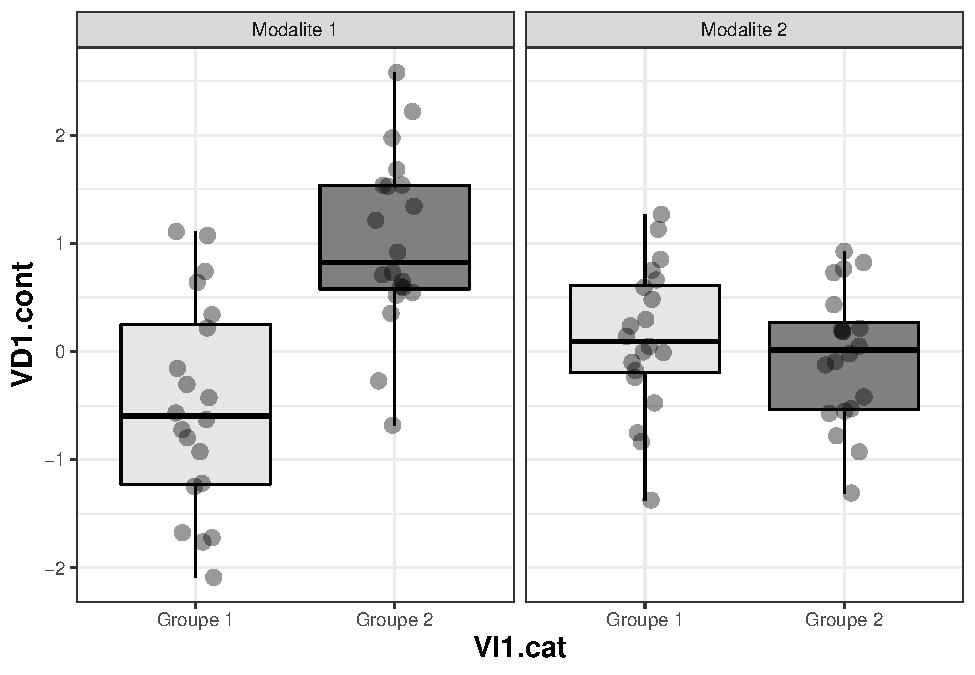
\includegraphics{Manuel_R_independant_files/figure-latex/unnamed-chunk-38-1.pdf}

\hypertarget{interpretation-3}{%
\subsubsection{Interpretation}\label{interpretation-3}}

{[}1{]} ``L'interaction entre VI1.cat et VI2.cat est significative (F = 23.588, p = 6.24e-06). La différence entre les scores obtenus par le groupe 1 et le groupe 2 est significative pour la modalité 1 de VI2.cat (moyenne groupe 1 = -0.506, SD groupe 1 = 0.965, N groupe 1 = 20; moyenne groupe 2 = 1.014, SD groupe 2 = 0.806, N groupe 2 = 20; p = 3e-08, d de cohen = -1.71), mais pas pour la modalité 2 de VI2.cat (M.grp1 = 0.125, SD groupe 1 = 0.67, N groupe 1 = 20; M groupe 2 = -0.041, SD groupe 2 = 0.618, N groupe 2 = 20; p = 0.501, d de cohen = 0.258)''

\hypertarget{regression-linuxe9aire-multiple-1}{%
\subsection{Regression linéaire multiple 1}\label{regression-linuxe9aire-multiple-1}}

\hypertarget{type-de-variables-4}{%
\subsubsection{Type de variables}\label{type-de-variables-4}}

\textbf{Variable Dépendante :} Numérique
\textbf{Variables Indépendantes :} Numériques

\hypertarget{packages-nuxe9cessaires-4}{%
\subsubsection{Packages nécessaires}\label{packages-nuxe9cessaires-4}}

\begin{Shaded}
\begin{Highlighting}[]
\KeywordTok{library}\NormalTok{(ggplot2)}
\KeywordTok{library}\NormalTok{(GGally)}
\KeywordTok{library}\NormalTok{(rstatix)}
\KeywordTok{library}\NormalTok{(dplyr)}
\KeywordTok{library}\NormalTok{(effects)}
\KeywordTok{library}\NormalTok{(lm.beta)}
\end{Highlighting}
\end{Shaded}

\hypertarget{donnuxe9es-ruxe9elles-4}{%
\subsubsection{Données réelles}\label{donnuxe9es-ruxe9elles-4}}

\begin{Shaded}
\begin{Highlighting}[]
\CommentTok{# choisissez la ligne appropriée au format de votre fichier de données. }

\CommentTok{# si vos données sont dans un fichier .txt}
\NormalTok{my_data.regmult1 <-}\StringTok{ }\KeywordTok{read.delim}\NormalTok{(}\KeywordTok{file.choose}\NormalTok{())}

\CommentTok{# si vos données sont dans un fichier .csv}
\NormalTok{my_data.regmult1 <-}\StringTok{ }\KeywordTok{read.csv}\NormalTok{(}\KeywordTok{file.choose}\NormalTok{())}

\CommentTok{# si vos données sont dans un fichier .xls / .xlsx}
\NormalTok{my_data.regmult1 <-}\StringTok{ }\KeywordTok{read_excel}\NormalTok{(}\KeywordTok{file.choose}\NormalTok{())}

\CommentTok{# une fois vos données chargées, vous pouvez renommer vos noms de colonnes afin qu'ils correspondent à ceux utilisés dans le code ci-dessous}
\CommentTok{# Si vous ne souhaitez pas renommer vos noms de colonnes, sautez cette étape mais adaptez le code des parties suivantes en lui indiquant les noms de colonnes de vos données.}

\CommentTok{# On crée une nouvelle colonne pour votre variable dépendante continue (remplacez 'votre.nom.de.colonne' par le nom approprié)}
\NormalTok{my_data.regmult1}\OperatorTok{$}\NormalTok{VD1.cont <-}\StringTok{ }\NormalTok{my_data.regmult1}\OperatorTok{$}\StringTok{'votre.nom.de.colonne'}

\CommentTok{# On crée une nouvelle colonne pour votre variable indépendante continue (remplacez 'votre.nom.de.colonne' par le nom approprié)}
\NormalTok{my_data.regmult1}\OperatorTok{$}\NormalTok{VI1.cont <-}\StringTok{ }\NormalTok{my_data.regmult1}\OperatorTok{$}\StringTok{'votre.nom.de.colonne'}
\NormalTok{my_data.regmult1}\OperatorTok{$}\NormalTok{VI2.cont <-}\StringTok{ }\NormalTok{my_data.regmult1}\OperatorTok{$}\StringTok{'votre.nom.de.colonne'}
\end{Highlighting}
\end{Shaded}

\hypertarget{donnuxe9es-fictives-4}{%
\subsubsection{Données fictives}\label{donnuxe9es-fictives-4}}

\begin{Shaded}
\begin{Highlighting}[]
\KeywordTok{set.seed}\NormalTok{(}\DecValTok{4321}\NormalTok{)}
\NormalTok{regmult1 <-}\StringTok{ }\KeywordTok{rnorm}\NormalTok{(}\DecValTok{50}\NormalTok{)}\OperatorTok{*}\DecValTok{3}
\NormalTok{my_data.regmult1 <-}\StringTok{ }\KeywordTok{data.frame}\NormalTok{(}
  \DataTypeTok{VD1.cont =} \KeywordTok{rnorm}\NormalTok{(}\DecValTok{50}\NormalTok{)}\OperatorTok{*}\DecValTok{2} \OperatorTok{+}\StringTok{ }\DecValTok{1}\OperatorTok{*}\NormalTok{regmult1,}
  \DataTypeTok{VI1.cont =} \KeywordTok{rnorm}\NormalTok{(}\DecValTok{50}\NormalTok{)}\OperatorTok{+}\StringTok{ }\FloatTok{0.2}\OperatorTok{*}\NormalTok{regmult1,}
  \DataTypeTok{VI2.cont =} \KeywordTok{rnorm}\NormalTok{(}\DecValTok{50}\NormalTok{))}
\end{Highlighting}
\end{Shaded}

\hypertarget{duxe9claration-du-type-de-variables-3}{%
\subsubsection{Déclaration du type de variables}\label{duxe9claration-du-type-de-variables-3}}

\begin{Shaded}
\begin{Highlighting}[]
\NormalTok{my_data.regmult1}\OperatorTok{$}\NormalTok{VD1.cont <-}\StringTok{ }\KeywordTok{as.numeric}\NormalTok{(}\KeywordTok{as.character}\NormalTok{(my_data.regmult1}\OperatorTok{$}\NormalTok{VD1.cont))}
\NormalTok{my_data.regmult1}\OperatorTok{$}\NormalTok{VI1.cont <-}\StringTok{ }\KeywordTok{as.numeric}\NormalTok{(}\KeywordTok{as.character}\NormalTok{(my_data.regmult1}\OperatorTok{$}\NormalTok{VI1.cont))}
\NormalTok{my_data.regmult1}\OperatorTok{$}\NormalTok{VI2.cont <-}\StringTok{ }\KeywordTok{as.numeric}\NormalTok{(}\KeywordTok{as.character}\NormalTok{(my_data.regmult1}\OperatorTok{$}\NormalTok{VI2.cont))}
\end{Highlighting}
\end{Shaded}

\hypertarget{inspection-des-donnuxe9es-3}{%
\subsubsection{Inspection des données}\label{inspection-des-donnuxe9es-3}}

\begin{Shaded}
\begin{Highlighting}[]
\CommentTok{## Les graphiques situés sur la diagonale représentent la distribution des variables}
\CommentTok{## Les graphiques (ou les valeurs de corrélation) situés au dessus et en dessous de la diagonale représentent l'association entre les différentes variables}
\KeywordTok{ggpairs}\NormalTok{(my_data.regmult1,}
        \DataTypeTok{lower =} \KeywordTok{list}\NormalTok{(}\DataTypeTok{continuous =} \KeywordTok{wrap}\NormalTok{(}\StringTok{"smooth"}\NormalTok{, }\DataTypeTok{alpha =} \FloatTok{0.7}\NormalTok{), }\DataTypeTok{combo =} \StringTok{"box_no_facet"}\NormalTok{),}
        \DataTypeTok{upper =} \KeywordTok{list}\NormalTok{(}\DataTypeTok{combo =} \StringTok{"facetdensity"}\NormalTok{, }\DataTypeTok{discrete =} \StringTok{"facetbar"}\NormalTok{), }
        \DataTypeTok{mapping =} \KeywordTok{aes}\NormalTok{(}\DataTypeTok{alpha =} \FloatTok{0.8}\NormalTok{)) }\OperatorTok{+}\StringTok{ }\KeywordTok{theme_bw}\NormalTok{()}
\end{Highlighting}
\end{Shaded}

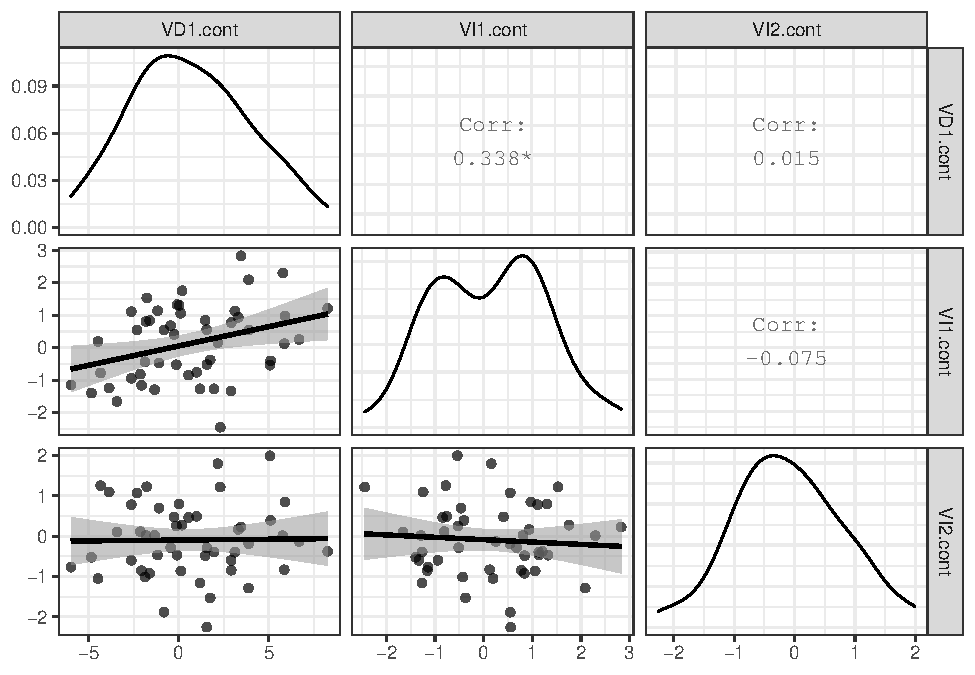
\includegraphics{Manuel_R_independant_files/figure-latex/unnamed-chunk-44-1.pdf}

\hypertarget{analyse-des-donnuxe9es-4}{%
\subsubsection{Analyse des données}\label{analyse-des-donnuxe9es-4}}

\begin{Shaded}
\begin{Highlighting}[]
\CommentTok{# calcul de la régression multiple et stockage des résultats dans l’objet regmult1.test}
\NormalTok{regmult1.test <-}\StringTok{ }\KeywordTok{lm}\NormalTok{(}\DataTypeTok{formula =}\NormalTok{ VD1.cont }\OperatorTok{~}\StringTok{ }\NormalTok{VI1.cont }\OperatorTok{+}\StringTok{ }\NormalTok{VI2.cont, }
                 \DataTypeTok{data =}\NormalTok{ my_data.regmult1)}

\CommentTok{# obtention des résultats de la régression linéaire multiple }

\CommentTok{## coefficients non-standardisés}
\KeywordTok{summary}\NormalTok{(regmult1.test)}
\end{Highlighting}
\end{Shaded}

\begin{verbatim}
## 
## Call:
## lm(formula = VD1.cont ~ VI1.cont + VI2.cont, data = my_data.regmult1)
## 
## Residuals:
##     Min      1Q  Median      3Q     Max 
## -5.2632 -2.1164 -0.3808  1.8615  6.6408 
## 
## Coefficients:
##             Estimate Std. Error t value Pr(>|t|)  
## (Intercept)   0.5084     0.4494   1.131   0.2636  
## VI1.cont      0.9693     0.3908   2.481   0.0168 *
## VI2.cont      0.1477     0.4984   0.296   0.7682  
## ---
## Signif. codes:  0 '***' 0.001 '**' 0.01 '*' 0.05 '.' 0.1 ' ' 1
## 
## Residual standard error: 3.143 on 47 degrees of freedom
## Multiple R-squared:  0.116,	Adjusted R-squared:  0.07835 
## F-statistic: 3.083 on 2 and 47 DF,  p-value: 0.05521
\end{verbatim}

\begin{Shaded}
\begin{Highlighting}[]
\CommentTok{## coefficients standardisés}
\KeywordTok{lm.beta}\NormalTok{(regmult1.test)}
\end{Highlighting}
\end{Shaded}

\begin{verbatim}
## 
## Call:
## lm(formula = VD1.cont ~ VI1.cont + VI2.cont, data = my_data.regmult1)
## 
## Standardized Coefficients::
## (Intercept)    VI1.cont    VI2.cont 
##  0.00000000  0.34115683  0.04076203
\end{verbatim}

\hypertarget{graphique-4}
\NormalTok{adjusted.slope.regmult1 <-}\StringTok{ }\KeywordTok{as.data.frame}\NormalTok{(}
  \KeywordTok{effect}\NormalTok{(}
    \DataTypeTok{term =} \StringTok{"VI1.cont"}\NormalTok{, }
    \DataTypeTok{mod =}\NormalTok{ regmult1.test))}

\KeywordTok{ggplot}\NormalTok{(my_data.regmult1, }\KeywordTok{aes}\NormalTok{(}\DataTypeTok{x =}\NormalTok{ VI1.cont, }\DataTypeTok{y =}\NormalTok{ VD1.cont)) }\OperatorTok{+}
\StringTok{  }\KeywordTok{geom_point}\NormalTok{(}\DataTypeTok{size =} \DecValTok{3}\NormalTok{, }\DataTypeTok{alpha =} \FloatTok{0.4}\NormalTok{) }\OperatorTok{+}\StringTok{ }
\StringTok{  }\KeywordTok{geom_ribbon}\NormalTok{(}\DataTypeTok{data =}\NormalTok{ adjusted.slope.regmult1, }
              \KeywordTok{aes}\NormalTok{(}\DataTypeTok{x =}\NormalTok{ VI1.cont, }\DataTypeTok{y =}\NormalTok{ fit, }\DataTypeTok{ymin =}\NormalTok{ lower, }\DataTypeTok{ymax =}\NormalTok{ upper), }
              \DataTypeTok{fill=}\StringTok{"grey"}\NormalTok{, }\DataTypeTok{alpha  =} \FloatTok{0.8}\NormalTok{) }\OperatorTok{+}
\StringTok{  }\KeywordTok{geom_line}\NormalTok{(}\DataTypeTok{data =}\NormalTok{ adjusted.slope.regmult1, }
            \KeywordTok{aes}\NormalTok{(}\DataTypeTok{x =}\NormalTok{ VI1.cont , }\DataTypeTok{y =}\NormalTok{ fit), }
            \DataTypeTok{color =} \StringTok{"black"}\NormalTok{, }\DataTypeTok{size =} \DecValTok{1}\NormalTok{) }\OperatorTok{+}
\StringTok{  }\KeywordTok{ylab}\NormalTok{(}\StringTok{"VD1.cont"}\NormalTok{) }\OperatorTok{+}\StringTok{ }\KeywordTok{xlab}\NormalTok{(}\StringTok{"VI1.cont"}\NormalTok{) }\OperatorTok{+}\StringTok{ }
\StringTok{  }\KeywordTok{theme_bw}\NormalTok{() }\OperatorTok{+}\StringTok{ }
\StringTok{  }\KeywordTok{theme}\NormalTok{(}\DataTypeTok{axis.title.y =} \KeywordTok{element_text}\NormalTok{(}\DataTypeTok{size =} \DecValTok{14}\NormalTok{, }\DataTypeTok{hjust =} \FloatTok{0.5}\NormalTok{, }\DataTypeTok{face=}\StringTok{"bold"}\NormalTok{), }
        \DataTypeTok{axis.title.x =} \KeywordTok{element_text}\NormalTok{(}\DataTypeTok{face=}\StringTok{"bold"}\NormalTok{, }\DataTypeTok{size =} \DecValTok{14}\NormalTok{, }\DataTypeTok{hjust =} \FloatTok{0.5}\NormalTok{))}
\end{Highlighting}
\end{Shaded}

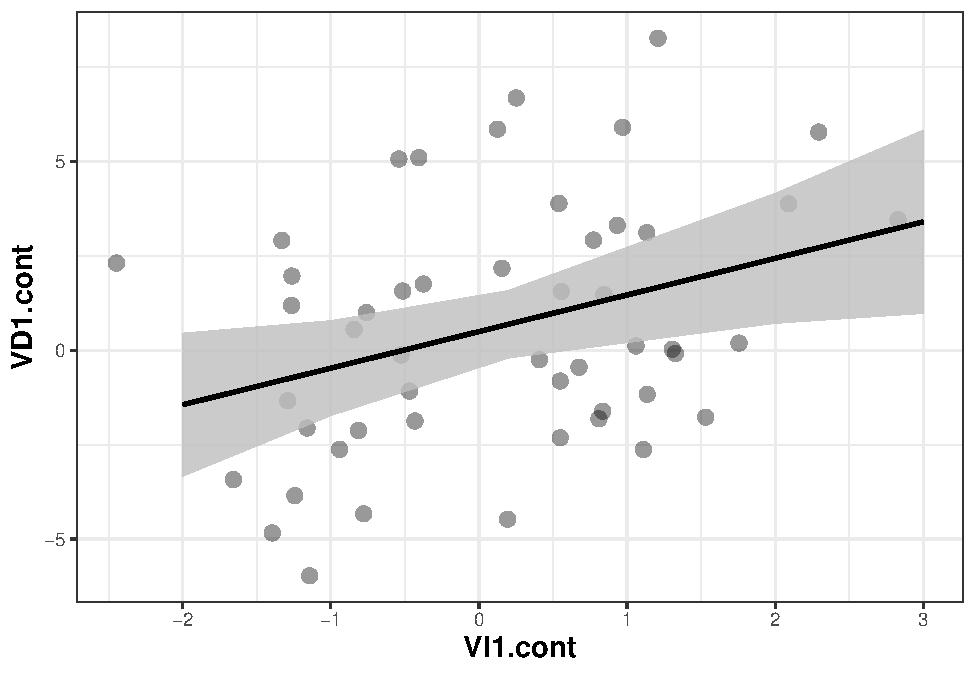
\includegraphics{Manuel_R_independant_files/figure-latex/unnamed-chunk-46-1.pdf}

\hypertarget{interpretation-4}{%
\subsubsection{Interpretation}\label{interpretation-4}}

{[}1{]} ``VI1.cont est significativement associé à VD1.cont même si l'on ajuste par l'effet de VI2.cont (b = 0.969, SE = 0.391, beta = 0.341, p = 0.017, N = 50)''

\hypertarget{ancova}{%
\subsection{ANCOVA}\label{ancova}}

ATTENTION : si votre variable indépendante principale est \textbf{Numérique} OU que vous faites une hypothèse d'interaction entre votre VI principale catégorielle et une autre covariable, reportez-vous à la section suivante \textbf{Régression linéaire multiple 2}.
Dans le cas contraire (votre VI principale est catégorielle ET vous ne faites pas d'hypothèse d'interaction entre votre VI catégorielle et une covariable), utilisez une ANCOVA décrite dans cette vignette.

\hypertarget{type-de-variables-5}{%
\subsubsection{Type de variables}\label{type-de-variables-5}}

\textbf{Variable Dépendante :} Numérique
\textbf{Variable indépendante principale:} Catégorielle (2 catégories ou +)
\textbf{Autres variables indépendantes (covariables) :} Numériques / Catégorielles

\hypertarget{packages-nuxe9cessaires-5}{%
\subsubsection{Packages nécessaires}\label{packages-nuxe9cessaires-5}}

\begin{Shaded}
\begin{Highlighting}[]
\KeywordTok{library}\NormalTok{(ggplot2)}
\KeywordTok{library}\NormalTok{(GGally)}
\KeywordTok{library}\NormalTok{(emmeans)}
\KeywordTok{library}\NormalTok{(effects)}
\KeywordTok{library}\NormalTok{(car)}
\KeywordTok{library}\NormalTok{(forcats)}
\KeywordTok{library}\NormalTok{(esc)}
\end{Highlighting}
\end{Shaded}

\hypertarget{donnuxe9es-ruxe9elles-5}{%
\subsubsection{Données réelles}\label{donnuxe9es-ruxe9elles-5}}

\begin{Shaded}
\begin{Highlighting}[]
\CommentTok{# choisissez la ligne appropriée au format de votre fichier de données. }

\CommentTok{# si vos données sont dans un fichier .txt}
\NormalTok{my_data.ancova <-}\StringTok{ }\KeywordTok{read.delim}\NormalTok{(}\KeywordTok{file.choose}\NormalTok{())}

\CommentTok{# si vos données sont dans un fichier .csv}
\NormalTok{my_data.ancova <-}\StringTok{ }\KeywordTok{read.csv}\NormalTok{(}\KeywordTok{file.choose}\NormalTok{())}

\CommentTok{# si vos données sont dans un fichier .xls / .xlsx}
\NormalTok{my_data.ancova <-}\StringTok{ }\KeywordTok{read_excel}\NormalTok{(}\KeywordTok{file.choose}\NormalTok{())}

\CommentTok{# une fois vos données chargées, vous pouvez renommer vos noms de colonnes afin qu'ils correspondent à ceux utilisés dans le code ci-dessous}
\CommentTok{# Si vous ne souhaitez pas renommer vos noms de colonnes, sautez cette étape mais adaptez le code des parties suivantes en lui indiquant les noms de colonnes de vos données.}

\CommentTok{# On crée une nouvelle colonne pour votre variable dépendante continue (remplacez 'votre.nom.de.colonne' par le nom approprié)}
\NormalTok{my_data.ancova}\OperatorTok{$}\NormalTok{VD1.cont <-}\StringTok{ }\NormalTok{my_data.ancova}\OperatorTok{$}\StringTok{'votre.nom.de.colonne'}

\CommentTok{# On crée une nouvelle colonne pour votre variable indépendante catégorielle (remplacez 'votre.nom.de.colonne' par le nom approprié)}
\NormalTok{my_data.ancova}\OperatorTok{$}\NormalTok{VI1.cat <-}\StringTok{ }\NormalTok{my_data.ancova}\OperatorTok{$}\StringTok{'votre.nom.de.colonne'}

\CommentTok{# On crée une nouvelle colonne pour votre variable indépendante continue (remplacez 'votre.nom.de.colonne' par le nom approprié)}
\NormalTok{my_data.ancova}\OperatorTok{$}\NormalTok{VI2.cont <-}\StringTok{ }\NormalTok{my_data.ancova}\OperatorTok{$}\StringTok{'votre.nom.de.colonne'}
\end{Highlighting}
\end{Shaded}

\hypertarget{donnuxe9es-fictives-5}{%
\subsubsection{Données fictives}\label{donnuxe9es-fictives-5}}

\begin{Shaded}
\begin{Highlighting}[]
\KeywordTok{set.seed}\NormalTok{(}\DecValTok{4321}\NormalTok{)}
\NormalTok{ancova <-}\StringTok{ }\KeywordTok{rnorm}\NormalTok{(}\DecValTok{200}\NormalTok{)}
\NormalTok{my_data.ancova <-}\StringTok{ }\KeywordTok{data.frame}\NormalTok{(}
  \DataTypeTok{VD1.cont =} \KeywordTok{rnorm}\NormalTok{(}\DecValTok{200}\NormalTok{) }\OperatorTok{+}\StringTok{ }\FloatTok{0.8}\OperatorTok{*}\NormalTok{ancova,}
  \DataTypeTok{VI1.cat =} \KeywordTok{rep}\NormalTok{(}\KeywordTok{c}\NormalTok{(}\DecValTok{1}\NormalTok{, }\DecValTok{2}\NormalTok{), }\DataTypeTok{each =} \DecValTok{100}\NormalTok{),}
  \DataTypeTok{VI2.cont =} \KeywordTok{c}\NormalTok{(}\KeywordTok{rnorm}\NormalTok{(}\DecValTok{200}\NormalTok{)}\OperatorTok{+}\FloatTok{0.8}\OperatorTok{*}\NormalTok{ancova))}

\CommentTok{# on renomme les catégories de VI1.cat pour que les résultats soient plus lisibles}
\NormalTok{my_data.ancova}\OperatorTok{$}\NormalTok{VI1.cat <-}\StringTok{ }\KeywordTok{fct_recode}\NormalTok{(}\KeywordTok{factor}\NormalTok{(my_data.ancova}\OperatorTok{$}\NormalTok{VI1.cat), }
                                        \StringTok{"Groupe 1"}\NormalTok{ =}\StringTok{ "1"}\NormalTok{, }
                                        \StringTok{"Groupe 2"}\NormalTok{ =}\StringTok{ "2"}\NormalTok{) }
\end{Highlighting}
\end{Shaded}

\hypertarget{duxe9claration-du-type-de-variables-4}{%
\subsubsection{Déclaration du type de variables}\label{duxe9claration-du-type-de-variables-4}}

\begin{Shaded}
\begin{Highlighting}[]
\NormalTok{my_data.ancova}\OperatorTok{$}\NormalTok{VD1.cont <-}\StringTok{ }\KeywordTok{as.numeric}\NormalTok{(}\KeywordTok{as.character}\NormalTok{(my_data.ancova}\OperatorTok{$}\NormalTok{VD1.cont))}
\NormalTok{my_data.ancova}\OperatorTok{$}\NormalTok{VI1.cat <-}\StringTok{ }\KeywordTok{factor}\NormalTok{(my_data.ancova}\OperatorTok{$}\NormalTok{VI1.cat)}
\NormalTok{my_data.ancova}\OperatorTok{$}\NormalTok{VI2.cont <-}\StringTok{ }\KeywordTok{as.numeric}\NormalTok{(}\KeywordTok{as.character}\NormalTok{(my_data.ancova}\OperatorTok{$}\NormalTok{VI2.cont))}
\end{Highlighting}
\end{Shaded}

\hypertarget{inspection-des-donnuxe9es-4}{%
\subsubsection{Inspection des données}\label{inspection-des-donnuxe9es-4}}

\begin{Shaded}
\begin{Highlighting}[]
\CommentTok{## Les graphiques situés sur la diagonale représentent la distribution des variables}
\CommentTok{## Les graphiques (ou les valeurs de corrélation) situés au dessus et en dessous de la diagonale représentent l'association entre les différentes variables}
\KeywordTok{ggpairs}\NormalTok{(my_data.ancova,}
        \DataTypeTok{lower =} \KeywordTok{list}\NormalTok{(}\DataTypeTok{continuous =} \KeywordTok{wrap}\NormalTok{(}\StringTok{"smooth"}\NormalTok{, }\DataTypeTok{alpha =} \FloatTok{0.7}\NormalTok{), }\DataTypeTok{combo =} \StringTok{"box_no_facet"}\NormalTok{),}
        \DataTypeTok{upper =} \KeywordTok{list}\NormalTok{(}\DataTypeTok{combo =} \StringTok{"facetdensity"}\NormalTok{, }\DataTypeTok{discrete =} \StringTok{"facetbar"}\NormalTok{), }
        \DataTypeTok{mapping =} \KeywordTok{aes}\NormalTok{(}\DataTypeTok{alpha =} \FloatTok{0.8}\NormalTok{)) }\OperatorTok{+}\StringTok{ }\KeywordTok{theme_bw}\NormalTok{()}
\end{Highlighting}
\end{Shaded}

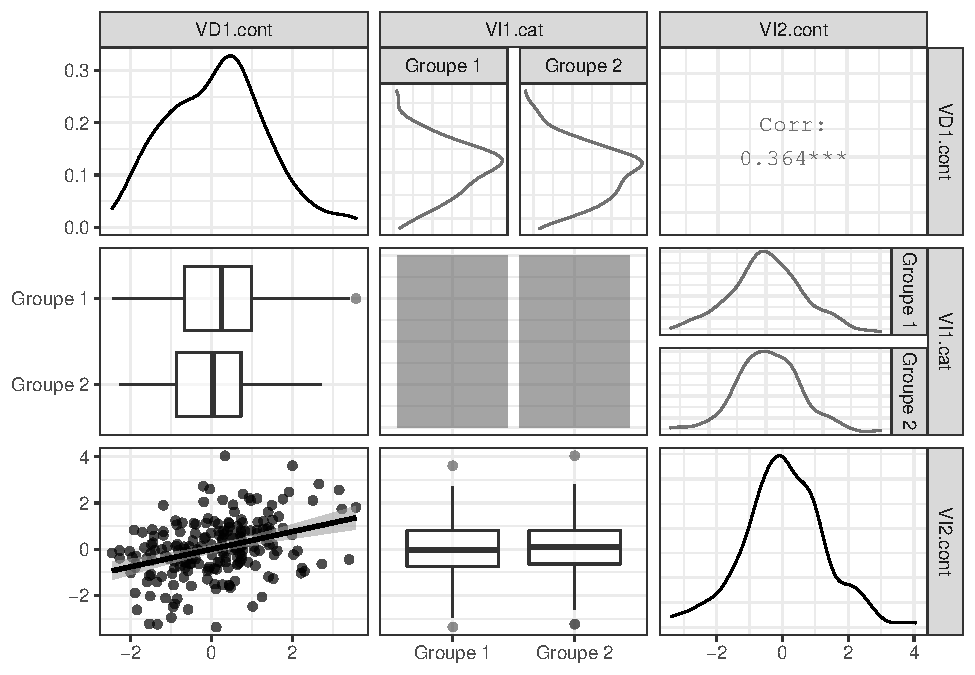
\includegraphics{Manuel_R_independant_files/figure-latex/unnamed-chunk-52-1.pdf}

\hypertarget{analyse-des-donnuxe9es-5}{%
\subsubsection{Analyse des données}\label{analyse-des-donnuxe9es-5}}

\begin{Shaded}
\begin{Highlighting}[]
\CommentTok{# calcul de l'ANCOVA et stockage des résultats dans l’objet ancova.test}
\NormalTok{ancova.test <-}\StringTok{ }\KeywordTok{lm}\NormalTok{(}\DataTypeTok{formula =}\NormalTok{ VD1.cont }\OperatorTok{~}\StringTok{ }\NormalTok{VI1.cat }\OperatorTok{+}\StringTok{ }\NormalTok{VI2.cont,}
                     \DataTypeTok{data =}\NormalTok{ my_data.ancova)}

\CommentTok{# calcul des moyennes marginales estimées et écarts types pour chaque modalité de VI1.cat}
\NormalTok{description.anovafact <-}\StringTok{ }\KeywordTok{emmeans}\NormalTok{(ancova.test, }\OperatorTok{~}\NormalTok{VI1.cat)}

\CommentTok{# calcul de la taille d'effet de VI1.cat sur VD1.cont (SMD/d de cohen ajusté par VI2.cont)}
\NormalTok{cohensd.ancova <-}\StringTok{ }\KeywordTok{esc_mean_se}\NormalTok{(}
  \DataTypeTok{grp1m =} \KeywordTok{summary}\NormalTok{(description.anovafact)}\OperatorTok{$}\NormalTok{emmean[}\DecValTok{1}\NormalTok{],}
  \DataTypeTok{grp1se =} \KeywordTok{summary}\NormalTok{(description.anovafact)}\OperatorTok{$}\NormalTok{SE[}\DecValTok{1}\NormalTok{],}
  \DataTypeTok{grp1n =} \KeywordTok{nrow}\NormalTok{(}\KeywordTok{subset}\NormalTok{(my_data.ancova, VI1.cat }\OperatorTok{==}\StringTok{ "Groupe 1"}\NormalTok{)),}
  \DataTypeTok{grp2m =} \KeywordTok{summary}\NormalTok{(description.anovafact)}\OperatorTok{$}\NormalTok{emmean[}\DecValTok{2}\NormalTok{],}
  \DataTypeTok{grp2se =} \KeywordTok{summary}\NormalTok{(description.anovafact)}\OperatorTok{$}\NormalTok{SE[}\DecValTok{2}\NormalTok{],}
  \DataTypeTok{grp2n =} \KeywordTok{nrow}\NormalTok{(}\KeywordTok{subset}\NormalTok{(my_data.ancova, VI1.cat }\OperatorTok{==}\StringTok{ "Groupe 2"}\NormalTok{)),}
  \DataTypeTok{es.type =} \StringTok{"d"}\NormalTok{)}

\CommentTok{# obtention des différentes moyennes/écarts-types }
\NormalTok{description.anovafact}
\end{Highlighting}
\end{Shaded}

\begin{verbatim}
##  VI1.cat   emmean    SE  df lower.CL upper.CL
##  Groupe 1  0.2580 0.113 197   0.0359    0.480
##  Groupe 2 -0.0369 0.113 197  -0.2591    0.185
## 
## Confidence level used: 0.95
\end{verbatim}

\begin{Shaded}
\begin{Highlighting}[]
\CommentTok{# obtention des résultats de l'anova }
\KeywordTok{Anova}\NormalTok{(ancova.test, }\DataTypeTok{type =} \DecValTok{2}\NormalTok{)}
\end{Highlighting}
\end{Shaded}

\begin{verbatim}
## Anova Table (Type II tests)
## 
## Response: VD1.cont
##            Sum Sq  Df F value   Pr(>F)    
## VI1.cat     4.349   1  3.4289  0.06556 .  
## VI2.cont   39.391   1 31.0605 8.15e-08 ***
## Residuals 249.838 197                     
## ---
## Signif. codes:  0 '***' 0.001 '**' 0.01 '*' 0.05 '.' 0.1 ' ' 1
\end{verbatim}

\begin{Shaded}
\begin{Highlighting}[]
\CommentTok{# obtention des tailles d'effet }
\NormalTok{cohensd.ancova}
\end{Highlighting}
\end{Shaded}

\begin{verbatim}
## 
## Effect Size Calculation for Meta Analysis
## 
##      Conversion: mean and se to effect size d
##     Effect Size:   0.2632
##  Standard Error:   0.1420
##        Variance:   0.0202
##        Lower CI:  -0.0152
##        Upper CI:   0.5416
##          Weight:  49.5707
\end{verbatim}

\hypertarget{graphique-5}{%
\subsubsection{Graphique}\label{graphique-5}}

\begin{Shaded}
\begin{Highlighting}[]
\CommentTok{# les barres d'erreurs représentent l'erreur standard.}
\NormalTok{adjusted.means.ancova <-}\StringTok{ }\KeywordTok{as.data.frame}\NormalTok{(}
  \KeywordTok{effect}\NormalTok{(}
    \DataTypeTok{term =} \StringTok{"VI1.cat"}\NormalTok{, }
    \DataTypeTok{mod =}\NormalTok{ ancova.test))}

\KeywordTok{ggplot}\NormalTok{(adjusted.means.ancova, }
       \KeywordTok{aes}\NormalTok{(}\DataTypeTok{x =}\NormalTok{ VI1.cat, }\DataTypeTok{y =}\NormalTok{ fit, }\DataTypeTok{fill =}\NormalTok{ VI1.cat)) }\OperatorTok{+}
\StringTok{  }\KeywordTok{geom_hline}\NormalTok{(}\KeywordTok{aes}\NormalTok{(}\DataTypeTok{yintercept =} \DecValTok{0}\NormalTok{)) }\OperatorTok{+}\StringTok{ }
\StringTok{  }\KeywordTok{geom_bar}\NormalTok{(}\DataTypeTok{stat =} \StringTok{"identity"}\NormalTok{, }\DataTypeTok{color =} \StringTok{"black"}\NormalTok{, }\DataTypeTok{alpha =} \FloatTok{0.7}\NormalTok{) }\OperatorTok{+}
\StringTok{  }\KeywordTok{geom_errorbar}\NormalTok{(}\KeywordTok{aes}\NormalTok{(}\DataTypeTok{ymin =}\NormalTok{ fit }\OperatorTok{-}\StringTok{ }\NormalTok{se, }
                    \DataTypeTok{ymax =}\NormalTok{ fit }\OperatorTok{+}\StringTok{ }\NormalTok{se), }
                \DataTypeTok{width =} \FloatTok{.1}\NormalTok{, }\DataTypeTok{col =} \StringTok{"black"}\NormalTok{) }\OperatorTok{+}
\StringTok{  }\KeywordTok{ylab}\NormalTok{(}\StringTok{"VD1.cont"}\NormalTok{) }\OperatorTok{+}\StringTok{ }\KeywordTok{xlab}\NormalTok{(}\StringTok{"VI1.cat"}\NormalTok{) }\OperatorTok{+}\StringTok{ }
\StringTok{  }\KeywordTok{theme_bw}\NormalTok{() }\OperatorTok{+}\StringTok{ }
\StringTok{  }\KeywordTok{theme}\NormalTok{(}\DataTypeTok{axis.title.y =} \KeywordTok{element_text}\NormalTok{(}\DataTypeTok{size =} \DecValTok{14}\NormalTok{, }\DataTypeTok{hjust =} \FloatTok{0.5}\NormalTok{, }\DataTypeTok{face =} \StringTok{"bold"}\NormalTok{), }
        \DataTypeTok{axis.title.x =} \KeywordTok{element_text}\NormalTok{(}\DataTypeTok{face =} \StringTok{"bold"}\NormalTok{, }\DataTypeTok{size =} \DecValTok{14}\NormalTok{, }\DataTypeTok{hjust =} \FloatTok{0.5}\NormalTok{)) }\OperatorTok{+}\StringTok{ }
\StringTok{  }\KeywordTok{scale_fill_grey}\NormalTok{(}\DataTypeTok{start =} \FloatTok{0.9}\NormalTok{, }\DataTypeTok{end =} \FloatTok{0.5}\NormalTok{) }\OperatorTok{+}
\StringTok{  }\KeywordTok{guides}\NormalTok{(}\DataTypeTok{fill =} \OtherTok{FALSE}\NormalTok{)}
\end{Highlighting}
\end{Shaded}

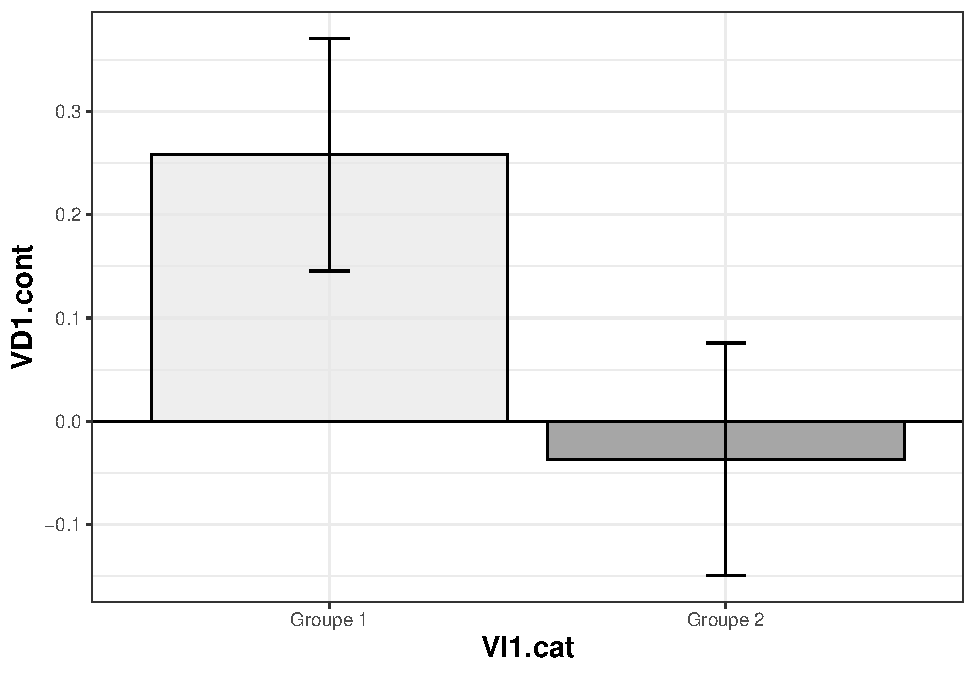
\includegraphics{Manuel_R_independant_files/figure-latex/unnamed-chunk-54-1.pdf}

\hypertarget{interpretation-5}{%
\subsubsection{Interpretation}\label{interpretation-5}}

{[}1{]} ``Les scores obtenus par le groupe 1 (moyenne groupe 1 = 0.258, SE groupe 1 = 0.113, N groupe 1 = 100) et le groupe 2 (moyenne groupe 2 = -0.037, SE groupe 2 = 0.113, N groupe 2 = 100) diffèrent de façon marginale lorsque la diférence est ajustée par l'effet de VI2.cont (F = 3.429, p = 0.066, d de cohen = 0.263)''

\hypertarget{regression-linuxe9aire-multiple-2}{%
\subsection{Regression linéaire multiple 2}\label{regression-linuxe9aire-multiple-2}}

ATTENTION : si votre variable indépendante principale est \textbf{catégorielle} ET que vous ne faites pas d'hypothèse d'interaction entre cette VI principale catégorielle et une autre covariable, reportez-vous à la section précédente \textbf{MANCOVA}.
Dans le cas contraire (votre VI principale est Numérique OU vous faites une hypothèse d'interaction entre votre VI catégorielle et une covariable), utilisez une régression linéaire décrite dans cette vignette.

\hypertarget{type-de-variables-6}{%
\subsubsection{Type de variables}\label{type-de-variables-6}}

\textbf{Variable Dépendante :} Numérique
\textbf{Variable indépendante principale:} Numérique
\textbf{Autres variables indépendantes :} Numériques / Catégorielles

\hypertarget{packages-nuxe9cessaires-6}{%
\subsubsection{Packages nécessaires}\label{packages-nuxe9cessaires-6}}

\begin{Shaded}
\begin{Highlighting}[]
\KeywordTok{library}\NormalTok{(ggplot2)}
\KeywordTok{library}\NormalTok{(GGally)}
\KeywordTok{library}\NormalTok{(rstatix)}
\KeywordTok{library}\NormalTok{(dplyr)}
\KeywordTok{library}\NormalTok{(effects)}
\KeywordTok{library}\NormalTok{(lm.beta)}
\end{Highlighting}
\end{Shaded}

\hypertarget{donnuxe9es-ruxe9elles-6}{%
\subsubsection{Données réelles}\label{donnuxe9es-ruxe9elles-6}}

\begin{Shaded}
\begin{Highlighting}[]
\CommentTok{# choisissez la ligne appropriée au format de votre fichier de données. }

\CommentTok{# si vos données sont dans un fichier .txt}
\NormalTok{my_data.regmult2 <-}\StringTok{ }\KeywordTok{read.delim}\NormalTok{(}\KeywordTok{file.choose}\NormalTok{())}

\CommentTok{# si vos données sont dans un fichier .csv}
\NormalTok{my_data.regmult2 <-}\StringTok{ }\KeywordTok{read.csv}\NormalTok{(}\KeywordTok{file.choose}\NormalTok{())}

\CommentTok{# si vos données sont dans un fichier .xls / .xlsx}
\NormalTok{my_data.regmult2 <-}\StringTok{ }\KeywordTok{read_excel}\NormalTok{(}\KeywordTok{file.choose}\NormalTok{())}

\CommentTok{# une fois vos données chargées, vous pouvez renommer vos noms de colonnes afin qu'ils correspondent à ceux utilisés dans le code ci-dessous}
\CommentTok{# Si vous ne souhaitez pas renommer vos noms de colonnes, sautez cette étape mais adaptez le code des parties suivantes en lui indiquant les noms de colonnes de vos données.}

\CommentTok{# On crée une nouvelle colonne pour votre variable dépendante continue (remplacez 'votre.nom.de.colonne' par le nom approprié)}
\NormalTok{my_data.regmult2}\OperatorTok{$}\NormalTok{VD1.cont <-}\StringTok{ }\NormalTok{my_data.regmult2}\OperatorTok{$}\StringTok{'votre.nom.de.colonne'}

\CommentTok{# On crée une nouvelle colonne pour votre variable indépendante continue (remplacez 'votre.nom.de.colonne' par le nom approprié)}
\NormalTok{my_data.regmult2}\OperatorTok{$}\NormalTok{VI1.cont <-}\StringTok{ }\NormalTok{my_data.regmult2}\OperatorTok{$}\StringTok{'votre.nom.de.colonne'}

\CommentTok{# On crée une nouvelle colonne pour votre variable indépendante catégorielle (remplacez 'votre.nom.de.colonne' par le nom approprié)}
\NormalTok{my_data.regmult2}\OperatorTok{$}\NormalTok{VI2.cat <-}\StringTok{ }\NormalTok{my_data.regmult2}\OperatorTok{$}\StringTok{'votre.nom.de.colonne'}
\end{Highlighting}
\end{Shaded}

\hypertarget{donnuxe9es-fictives-6}{%
\subsubsection{Données fictives}\label{donnuxe9es-fictives-6}}

\begin{Shaded}
\begin{Highlighting}[]
\KeywordTok{set.seed}\NormalTok{(}\DecValTok{4321}\NormalTok{)}
\NormalTok{my_data.regmult2 <-}\StringTok{ }\KeywordTok{data.frame}\NormalTok{(}
  \DataTypeTok{VD1.cont =} \KeywordTok{rnorm}\NormalTok{(}\DecValTok{150}\NormalTok{),}
  \DataTypeTok{VI1.cont =} \KeywordTok{rnorm}\NormalTok{(}\DecValTok{150}\NormalTok{),}
  \DataTypeTok{VI2.cat =} \KeywordTok{rbinom}\NormalTok{(}\DecValTok{150}\NormalTok{, }\DecValTok{2}\NormalTok{, }\FloatTok{0.4}\NormalTok{))}
\end{Highlighting}
\end{Shaded}

\hypertarget{duxe9claration-du-type-de-variables-5}{%
\subsubsection{Déclaration du type de variables}\label{duxe9claration-du-type-de-variables-5}}

\begin{Shaded}
\begin{Highlighting}[]
\NormalTok{my_data.regmult2}\OperatorTok{$}\NormalTok{VD1.cont <-}\StringTok{ }\KeywordTok{as.numeric}\NormalTok{(}\KeywordTok{as.character}\NormalTok{(my_data.regmult2}\OperatorTok{$}\NormalTok{VD1.cont))}
\NormalTok{my_data.regmult2}\OperatorTok{$}\NormalTok{VI1.cont <-}\StringTok{ }\KeywordTok{as.numeric}\NormalTok{(}\KeywordTok{as.character}\NormalTok{(my_data.regmult2}\OperatorTok{$}\NormalTok{VI1.cont))}
\NormalTok{my_data.regmult2}\OperatorTok{$}\NormalTok{VI2.cat <-}\StringTok{ }\KeywordTok{factor}\NormalTok{(my_data.regmult2}\OperatorTok{$}\NormalTok{VI2.cat)}
\end{Highlighting}
\end{Shaded}

\hypertarget{inspection-des-donnuxe9es-5}{%
\subsubsection{Inspection des données}\label{inspection-des-donnuxe9es-5}}

\begin{Shaded}
\begin{Highlighting}[]
\CommentTok{## Les graphiques situés sur la diagonale représentent la distribution des variables}
\CommentTok{## Les graphiques (ou les valeurs de corrélation) situés au dessus et en dessous de la diagonale représentent l'association entre les différentes variables}
\KeywordTok{ggpairs}\NormalTok{(my_data.regmult2,}
        \DataTypeTok{lower =} \KeywordTok{list}\NormalTok{(}\DataTypeTok{continuous =} \KeywordTok{wrap}\NormalTok{(}\StringTok{"smooth"}\NormalTok{, }\DataTypeTok{alpha =} \FloatTok{0.7}\NormalTok{), }\DataTypeTok{combo =} \StringTok{"box_no_facet"}\NormalTok{),}
        \DataTypeTok{upper =} \KeywordTok{list}\NormalTok{(}\DataTypeTok{combo =} \StringTok{"facetdensity"}\NormalTok{, }\DataTypeTok{discrete =} \StringTok{"facetbar"}\NormalTok{), }
        \DataTypeTok{mapping =} \KeywordTok{aes}\NormalTok{(}\DataTypeTok{alpha =} \FloatTok{0.8}\NormalTok{)) }\OperatorTok{+}\StringTok{ }\KeywordTok{theme_bw}\NormalTok{()}
\end{Highlighting}
\end{Shaded}

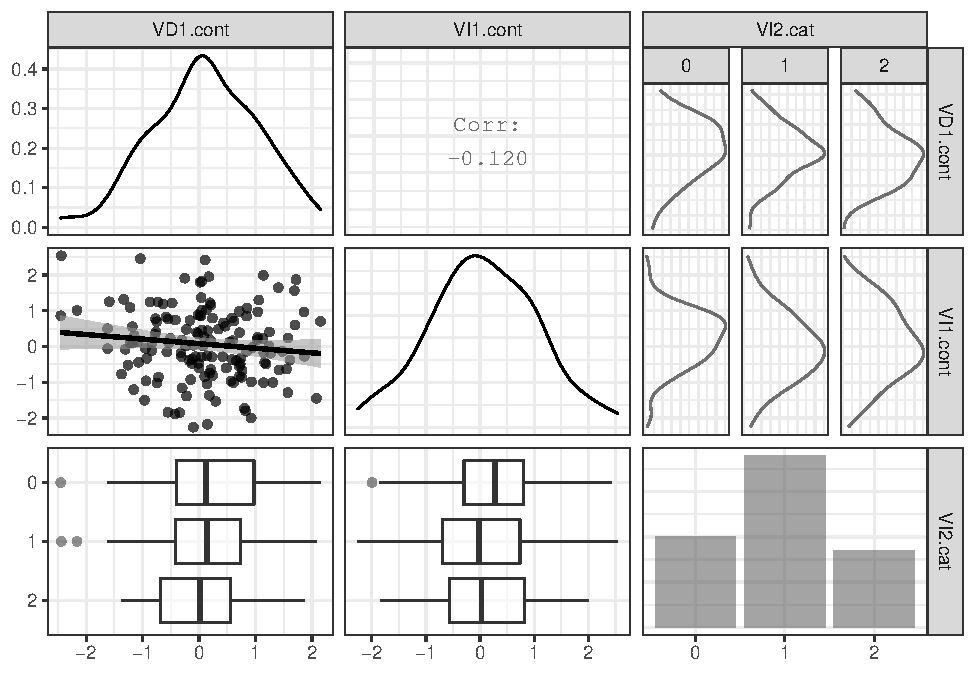
\includegraphics{Manuel_R_independant_files/figure-latex/unnamed-chunk-60-1.pdf}

\hypertarget{analyse-des-donnuxe9es-6}{%
\subsubsection{Analyse des données}\label{analyse-des-donnuxe9es-6}}

\begin{Shaded}
\begin{Highlighting}[]
\CommentTok{# calcul de la régression linéaire multiple et stockage des résultats dans l’objet regmult2.test}
\NormalTok{regmult2.test <-}\StringTok{ }\KeywordTok{lm}\NormalTok{(}\DataTypeTok{formula =}\NormalTok{ VD1.cont }\OperatorTok{~}\StringTok{ }\NormalTok{VI1.cont }\OperatorTok{+}\StringTok{ }\NormalTok{VI2.cat, }
                 \DataTypeTok{data =}\NormalTok{ my_data.regmult2)}

\CommentTok{# obtention des résultats de la régression linéaire multiple }

\CommentTok{## coefficients non-standardisés}
\KeywordTok{summary}\NormalTok{(regmult2.test)}
\end{Highlighting}
\end{Shaded}

\begin{verbatim}
## 
## Call:
## lm(formula = VD1.cont ~ VI1.cont + VI2.cat, data = my_data.regmult2)
## 
## Residuals:
##      Min       1Q   Median       3Q      Max 
## -2.54914 -0.62000  0.01413  0.57802  2.03373 
## 
## Coefficients:
##             Estimate Std. Error t value Pr(>|t|)
## (Intercept)  0.19946    0.14830   1.345    0.181
## VI1.cont    -0.11666    0.07727  -1.510    0.133
## VI2.cat1    -0.10452    0.18289  -0.572    0.569
## VI2.cat2    -0.16059    0.21770  -0.738    0.462
## 
## Residual standard error: 0.932 on 146 degrees of freedom
## Multiple R-squared:  0.01828,	Adjusted R-squared:  -0.001887 
## F-statistic: 0.9064 on 3 and 146 DF,  p-value: 0.4396
\end{verbatim}

\begin{Shaded}
\begin{Highlighting}[]
\CommentTok{## coefficients standardisés}
\KeywordTok{lm.beta}\NormalTok{(regmult2.test)}
\end{Highlighting}
\end{Shaded}

\begin{verbatim}
## 
## Call:
## lm(formula = VD1.cont ~ VI1.cont + VI2.cat, data = my_data.regmult2)
## 
## Standardized Coefficients::
## (Intercept)    VI1.cont    VI2.cat1    VI2.cat2 
##  0.00000000 -0.12437621 -0.05631223 -0.07245262
\end{verbatim}

\hypertarget{graphique-6}
\NormalTok{adjusted.slope.regmult2 <-}\StringTok{ }\KeywordTok{as.data.frame}\NormalTok{(}
  \KeywordTok{effect}\NormalTok{(}
    \DataTypeTok{term =} \StringTok{"VI1.cont"}\NormalTok{, }
    \DataTypeTok{mod =}\NormalTok{ regmult2.test))}

\KeywordTok{ggplot}\NormalTok{(my_data.regmult2, }\KeywordTok{aes}\NormalTok{(}\DataTypeTok{x =}\NormalTok{ VI1.cont, }\DataTypeTok{y =}\NormalTok{ VD1.cont)) }\OperatorTok{+}
\StringTok{  }\KeywordTok{geom_point}\NormalTok{(}\DataTypeTok{size =} \DecValTok{3}\NormalTok{, }\DataTypeTok{alpha =} \FloatTok{0.4}\NormalTok{) }\OperatorTok{+}\StringTok{ }
\StringTok{  }\KeywordTok{geom_ribbon}\NormalTok{(}\DataTypeTok{data =}\NormalTok{ adjusted.slope.regmult2, }
              \KeywordTok{aes}\NormalTok{(}\DataTypeTok{x =}\NormalTok{ VI1.cont, }\DataTypeTok{y =}\NormalTok{ fit, }\DataTypeTok{ymin =}\NormalTok{ lower, }\DataTypeTok{ymax =}\NormalTok{ upper), }
              \DataTypeTok{fill =} \StringTok{"grey"}\NormalTok{, }\DataTypeTok{alpha =} \FloatTok{0.8}\NormalTok{) }\OperatorTok{+}
\StringTok{  }\KeywordTok{geom_line}\NormalTok{(}\DataTypeTok{data =}\NormalTok{ adjusted.slope.regmult2, }
            \KeywordTok{aes}\NormalTok{(}\DataTypeTok{x =}\NormalTok{ VI1.cont , }\DataTypeTok{y =}\NormalTok{ fit), }
            \DataTypeTok{color =} \StringTok{"black"}\NormalTok{, }\DataTypeTok{size =} \DecValTok{1}\NormalTok{) }\OperatorTok{+}
\StringTok{  }\KeywordTok{ylab}\NormalTok{(}\StringTok{"VD1.cont"}\NormalTok{) }\OperatorTok{+}\StringTok{ }\KeywordTok{xlab}\NormalTok{(}\StringTok{"VI1.cont"}\NormalTok{) }\OperatorTok{+}\StringTok{ }
\StringTok{  }\KeywordTok{theme_bw}\NormalTok{() }\OperatorTok{+}\StringTok{ }
\StringTok{  }\KeywordTok{theme}\NormalTok{(}\DataTypeTok{axis.title.y =} \KeywordTok{element_text}\NormalTok{(}\DataTypeTok{size =} \DecValTok{14}\NormalTok{, }\DataTypeTok{hjust =} \FloatTok{0.5}\NormalTok{, }\DataTypeTok{face =} \StringTok{"bold"}\NormalTok{), }
        \DataTypeTok{axis.title.x =} \KeywordTok{element_text}\NormalTok{(}\DataTypeTok{face =} \StringTok{"bold"}\NormalTok{, }\DataTypeTok{size =} \DecValTok{14}\NormalTok{, }\DataTypeTok{hjust =} \FloatTok{0.5}\NormalTok{))}
\end{Highlighting}
\end{Shaded}

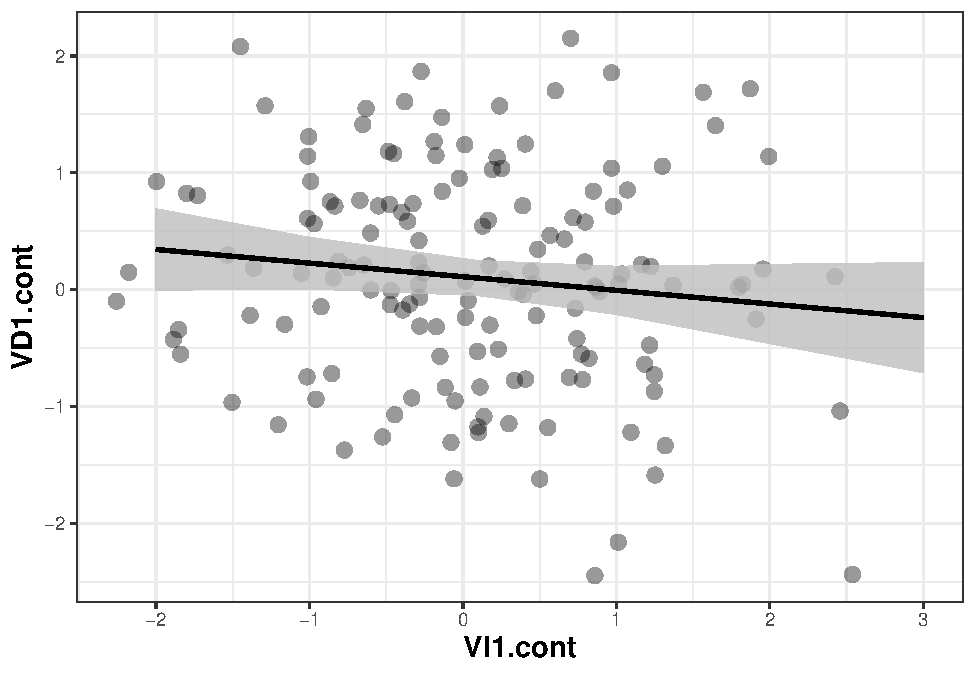
\includegraphics{Manuel_R_independant_files/figure-latex/unnamed-chunk-62-1.pdf}

\hypertarget{interpretation-6}{%
\subsubsection{Interpretation}\label{interpretation-6}}

{[}1{]} ``VI1.cont n'est pas significativement associée à VD1.cont lorsque l'on ajuste par l'effet de VI2.cat et VI3.cat (b = -0.117, SE = 0.077, beta = -0.124, p = 0.133, N = 150)''

\hypertarget{une-seule-vd-catuxe9gorielle}{%
\section{Une seule VD catégorielle}\label{une-seule-vd-catuxe9gorielle}}

\hypertarget{chi-deux-1}{%
\subsection{Chi-deux 1}\label{chi-deux-1}}

\hypertarget{type-de-variables-7}{%
\subsubsection{Type de variables}\label{type-de-variables-7}}

\textbf{Variable Dépendante :} Catégorielle (2 catégories)
\textbf{Variable Indépendante :} Catégorielle (2 catégories ou +)

\hypertarget{packages-nuxe9cessaires-7}{%
\subsubsection{Packages nécessaires}\label{packages-nuxe9cessaires-7}}

\begin{Shaded}
\begin{Highlighting}[]
\KeywordTok{library}\NormalTok{(ggplot2)}
\KeywordTok{library}\NormalTok{(GGally)}
\KeywordTok{library}\NormalTok{(forcats)}
\KeywordTok{library}\NormalTok{(dplyr)}
\end{Highlighting}
\end{Shaded}

\hypertarget{donnuxe9es-ruxe9elles-7}{%
\subsubsection{Données réelles}\label{donnuxe9es-ruxe9elles-7}}

\begin{Shaded}
\begin{Highlighting}[]
\CommentTok{# choisissez la ligne appropriée au format de votre fichier de données. }

\CommentTok{# si vos données sont dans un fichier .txt}
\NormalTok{my_data.chideux1 <-}\StringTok{ }\KeywordTok{read.delim}\NormalTok{(}\KeywordTok{file.choose}\NormalTok{())}

\CommentTok{# si vos données sont dans un fichier .csv}
\NormalTok{my_data.chideux1 <-}\StringTok{ }\KeywordTok{read.csv}\NormalTok{(}\KeywordTok{file.choose}\NormalTok{())}

\CommentTok{# si vos données sont dans un fichier .xls / .xlsx}
\NormalTok{my_data.chideux1 <-}\StringTok{ }\KeywordTok{read_excel}\NormalTok{(}\KeywordTok{file.choose}\NormalTok{())}

\CommentTok{# une fois vos données chargées, vous pouvez renommer vos noms de colonnes afin qu'ils correspondent à ceux utilisés dans le code ci-dessous}
\CommentTok{# Si vous ne souhaitez pas renommer vos noms de colonnes, sautez cette étape mais adaptez le code des parties suivantes en lui indiquant les noms de colonnes de vos données.}

\CommentTok{# On crée une nouvelle colonne pour votre variable dépendante catégorielle (remplacez 'votre.nom.de.colonne' par le nom approprié)}
\NormalTok{my_data.chideux1}\OperatorTok{$}\NormalTok{VD1.cat <-}\StringTok{ }\NormalTok{my_data.chideux1}\OperatorTok{$}\StringTok{'votre.nom.de.colonne'}

\CommentTok{# On crée une nouvelle colonne pour votre variable indépendante catégorielle (remplacez 'votre.nom.de.colonne' par le nom approprié)}
\NormalTok{my_data.chideux1}\OperatorTok{$}\NormalTok{VI1.cat <-}\StringTok{ }\NormalTok{my_data.chideux1}\OperatorTok{$}\StringTok{'votre.nom.de.colonne'}
\end{Highlighting}
\end{Shaded}

\hypertarget{donnuxe9es-fictives-7}{%
\subsubsection{Données fictives}\label{donnuxe9es-fictives-7}}

\begin{Shaded}
\begin{Highlighting}[]
\KeywordTok{set.seed}\NormalTok{(}\DecValTok{4321}\NormalTok{)}
\NormalTok{my_data.chideux1 <-}\StringTok{ }\KeywordTok{data.frame}\NormalTok{(}
  \DataTypeTok{VD1.cat =} \KeywordTok{rbinom}\NormalTok{(}\DecValTok{55}\NormalTok{, }\DecValTok{1}\NormalTok{, }\FloatTok{0.5}\NormalTok{) }\OperatorTok{+}\StringTok{ }\DecValTok{1}\NormalTok{,}
  \DataTypeTok{VI1.cat =} \KeywordTok{rbinom}\NormalTok{(}\DecValTok{55}\NormalTok{, }\DecValTok{1}\NormalTok{, }\FloatTok{0.3}\NormalTok{) }\OperatorTok{+}\StringTok{ }\DecValTok{1}\NormalTok{)}

\CommentTok{# on renomme les catégories de VD1.cat et VI1.cat pour que les résultats soient plus lisibles}
\NormalTok{my_data.chideux1}\OperatorTok{$}\NormalTok{VD1.cat <-}\StringTok{ }\KeywordTok{fct_recode}\NormalTok{(}\KeywordTok{factor}\NormalTok{(my_data.chideux1}\OperatorTok{$}\NormalTok{VD1.cat), }
                                    \StringTok{"Positif"}\NormalTok{ =}\StringTok{ "1"}\NormalTok{, }
                                    \StringTok{"Negatif"}\NormalTok{ =}\StringTok{ "2"}\NormalTok{) }

\NormalTok{my_data.chideux1}\OperatorTok{$}\NormalTok{VI1.cat <-}\StringTok{ }\KeywordTok{fct_recode}\NormalTok{(}\KeywordTok{factor}\NormalTok{(my_data.chideux1}\OperatorTok{$}\NormalTok{VI1.cat), }
                                    \StringTok{"Groupe 1"}\NormalTok{ =}\StringTok{ "1"}\NormalTok{, }
                                    \StringTok{"Groupe 2"}\NormalTok{ =}\StringTok{ "2"}\NormalTok{) }
\end{Highlighting}
\end{Shaded}

\hypertarget{duxe9claration-du-type-de-variables-6}{%
\subsubsection{Déclaration du type de variables}\label{duxe9claration-du-type-de-variables-6}}

\begin{Shaded}
\begin{Highlighting}[]
\NormalTok{my_data.chideux1}\OperatorTok{$}\NormalTok{VD1.cat <-}\StringTok{ }\KeywordTok{factor}\NormalTok{(my_data.chideux1}\OperatorTok{$}\NormalTok{VD1.cat)}
\NormalTok{my_data.chideux1}\OperatorTok{$}\NormalTok{VI1.cat <-}\StringTok{ }\KeywordTok{factor}\NormalTok{(my_data.chideux1}\OperatorTok{$}\NormalTok{VI1.cat)}
\end{Highlighting}
\end{Shaded}

\hypertarget{inspection-des-donnuxe9es-6}{%
\subsubsection{Inspection des données}\label{inspection-des-donnuxe9es-6}}

\begin{Shaded}
\begin{Highlighting}[]
\CommentTok{## Les graphiques situés sur la diagonale représentent la distribution des variables}
\CommentTok{## Les graphiques (ou les valeurs de corrélation) situés au dessus et en dessous de la diagonale représentent l'association entre les différentes variables}
\KeywordTok{ggpairs}\NormalTok{(my_data.chideux1,}
        \DataTypeTok{lower =} \KeywordTok{list}\NormalTok{(}\DataTypeTok{continuous =} \KeywordTok{wrap}\NormalTok{(}\StringTok{"smooth"}\NormalTok{, }\DataTypeTok{alpha =} \FloatTok{0.7}\NormalTok{), }\DataTypeTok{combo =} \StringTok{"box_no_facet"}\NormalTok{),}
        \DataTypeTok{upper =} \KeywordTok{list}\NormalTok{(}\DataTypeTok{combo =} \StringTok{"facetdensity"}\NormalTok{, }\DataTypeTok{discrete =} \StringTok{"facetbar"}\NormalTok{), }
        \DataTypeTok{mapping =} \KeywordTok{aes}\NormalTok{(}\DataTypeTok{alpha =} \FloatTok{0.8}\NormalTok{)) }\OperatorTok{+}\StringTok{ }\KeywordTok{theme_bw}\NormalTok{()}
\end{Highlighting}
\end{Shaded}

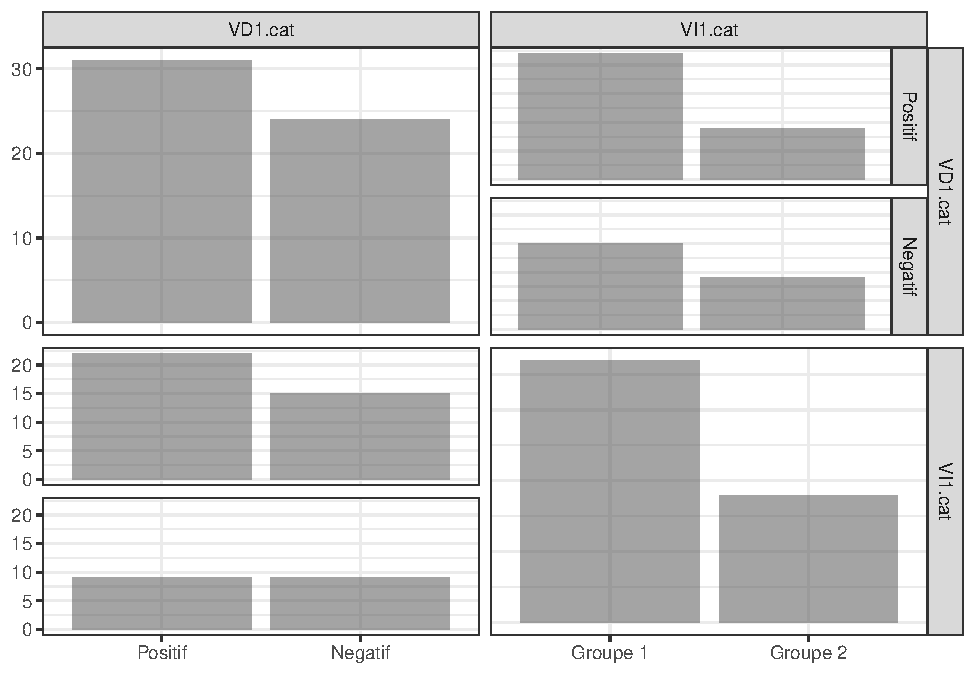
\includegraphics{Manuel_R_independant_files/figure-latex/unnamed-chunk-68-1.pdf}

\hypertarget{analyse-des-donnuxe9es-7}{%
\subsubsection{Analyse des données}\label{analyse-des-donnuxe9es-7}}

\begin{Shaded}
\begin{Highlighting}[]
\CommentTok{# on range les données sous forme de table }
\NormalTok{my_table.chideux1 <-}\StringTok{ }\KeywordTok{with}\NormalTok{(my_data.chideux1, }\KeywordTok{table}\NormalTok{(VI1.cat, VD1.cat))}

\CommentTok{# calcul du test de chi-deux et stockage des résultats dans l’objet chideux1.test}
\CommentTok{# la correction de Yates peut être obtenue en indiquant l'argument "correct = TRUE"}
\NormalTok{chideux1.test <-}\StringTok{ }\KeywordTok{chisq.test}\NormalTok{(my_table.chideux1, }\DataTypeTok{correct =} \OtherTok{FALSE}\NormalTok{)}

\CommentTok{# calcul des proportions de VD1.cat dans chaque modalité de VI1.cat}
\NormalTok{description.chideux1 <-}\StringTok{ }\KeywordTok{data.frame}\NormalTok{(my_table.chideux1) }\OperatorTok
\StringTok{    }\KeywordTok{group_by}\NormalTok{(VI1.cat) }\OperatorTok
\StringTok{    }\KeywordTok{summarise}\NormalTok{(}\DataTypeTok{proportion =}\NormalTok{ Freq }\OperatorTok{/}\StringTok{ }\KeywordTok{sum}\NormalTok{(Freq),}
              \DataTypeTok{VD1.cat =}\NormalTok{ VD1.cat)}

\CommentTok{# calcul de la taille d'effet de VI1.cat sur VD1.cat (odds ratio)}
\NormalTok{odds.ratio.chideux1 <-}\StringTok{ }\NormalTok{(my_table.chideux1[}\DecValTok{1}\NormalTok{,}\DecValTok{1}\NormalTok{]}\OperatorTok{/}\NormalTok{my_table.chideux1[}\DecValTok{1}\NormalTok{,}\DecValTok{2}\NormalTok{])}\OperatorTok{/}\NormalTok{(my_table.chideux1[}\DecValTok{2}\NormalTok{,}\DecValTok{1}\NormalTok{]}\OperatorTok{/}\NormalTok{my_table.chideux1[}\DecValTok{2}\NormalTok{,}\DecValTok{2}\NormalTok{])}

\CommentTok{# obtention des résultats tableau de contigence et des proportions  }
\NormalTok{my_table.chideux1; description.chideux1}
\end{Highlighting}
\end{Shaded}

\begin{verbatim}
##           VD1.cat
## VI1.cat    Positif Negatif
##   Groupe 1      22      15
##   Groupe 2       9       9
\end{verbatim}

\begin{verbatim}
## # A tibble: 4 x 3
## # Groups:   VI1.cat [2]
##   VI1.cat  proportion VD1.cat
##   <fct>         <dbl> <fct>  
## 1 Groupe 1      0.595 Positif
## 2 Groupe 1      0.405 Negatif
## 3 Groupe 2      0.5   Positif
## 4 Groupe 2      0.5   Negatif
\end{verbatim}

\begin{Shaded}
\begin{Highlighting}[]
\CommentTok{# obtention du test de chi deux }
\NormalTok{chideux1.test}
\end{Highlighting}
\end{Shaded}

\begin{verbatim}
## 
## 	Pearson's Chi-squared test
## 
## data:  my_table.chideux1
## X-squared = 0.44055, df = 1, p-value = 0.5069
\end{verbatim}

\begin{Shaded}
\begin{Highlighting}[]
\CommentTok{# obtention des tailles d'effet}
\NormalTok{odds.ratio.chideux1}
\end{Highlighting}
\end{Shaded}

\begin{verbatim}
## [1] 1.466667
\end{verbatim}

\hypertarget{graphique-7}{%
\subsubsection{Graphique}\label{graphique-7}}

\begin{Shaded}
\begin{Highlighting}[]
\KeywordTok{ggplot}\NormalTok{(my_data.chideux1, }\KeywordTok{aes}\NormalTok{(}\DataTypeTok{x =} \KeywordTok{factor}\NormalTok{(VI1.cat), }\DataTypeTok{fill =}\NormalTok{ VD1.cat)) }\OperatorTok{+}\StringTok{ }
\StringTok{  }\KeywordTok{geom_bar}\NormalTok{(}\DataTypeTok{stat =} \StringTok{"count"}\NormalTok{, }\DataTypeTok{position =} \KeywordTok{position_dodge2}\NormalTok{())  }\OperatorTok{+}
\StringTok{  }\KeywordTok{scale_fill_grey}\NormalTok{(}\DataTypeTok{start =} \FloatTok{0.8}\NormalTok{, }\DataTypeTok{end =} \FloatTok{0.5}\NormalTok{) }\OperatorTok{+}
\StringTok{  }\KeywordTok{ylab}\NormalTok{(}\StringTok{"Nombre de personnes"}\NormalTok{) }\OperatorTok{+}\StringTok{ }\KeywordTok{xlab}\NormalTok{(}\StringTok{"VI1.cat"}\NormalTok{) }\OperatorTok{+}\StringTok{ }
\StringTok{  }\KeywordTok{theme_bw}\NormalTok{() }\OperatorTok{+}\StringTok{ }
\StringTok{  }\KeywordTok{theme}\NormalTok{(}\DataTypeTok{axis.title.y =} \KeywordTok{element_text}\NormalTok{(}\DataTypeTok{size =} \DecValTok{14}\NormalTok{, }\DataTypeTok{hjust =} \FloatTok{0.5}\NormalTok{, }\DataTypeTok{face =} \StringTok{"bold"}\NormalTok{), }
        \DataTypeTok{axis.title.x =} \KeywordTok{element_text}\NormalTok{(}\DataTypeTok{face =} \StringTok{"bold"}\NormalTok{, }\DataTypeTok{size =} \DecValTok{14}\NormalTok{, }\DataTypeTok{hjust =} \FloatTok{0.5}\NormalTok{))}
\end{Highlighting}
\end{Shaded}

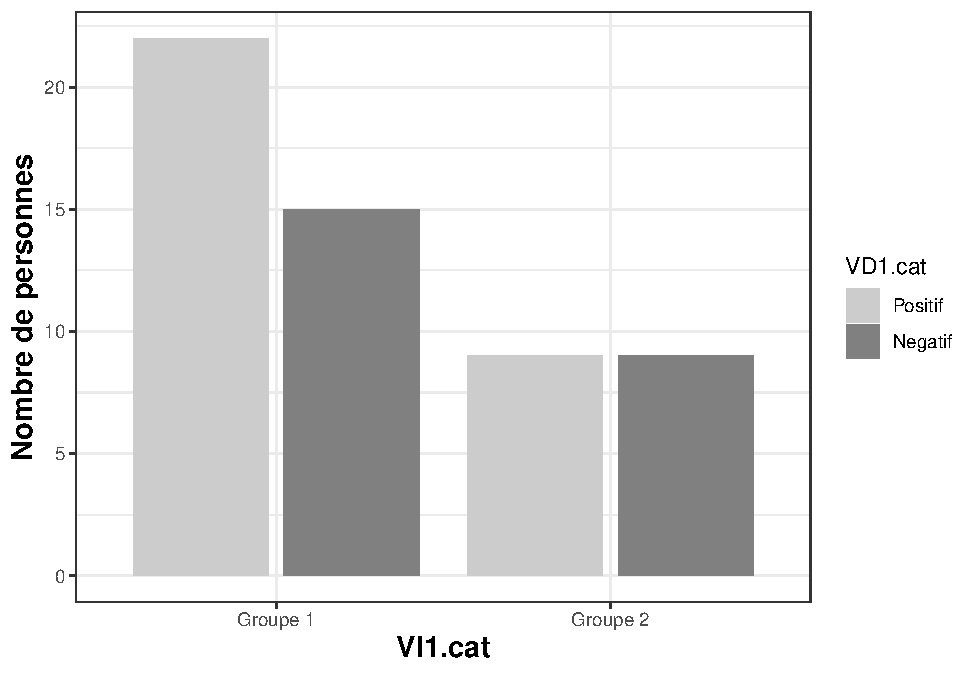
\includegraphics{Manuel_R_independant_files/figure-latex/unnamed-chunk-70-1.pdf}

\hypertarget{interpretation-7}{%
\subsubsection{Interpretation}\label{interpretation-7}}

{[}1{]} ``La proportion de cas ayant une modalité de VD1.cat égale à 1 (positif) ne diffère pas statistiquement entre les groupes 1 et 2 (groupe 1 = 59.5\%, groupe 2 = 50\%, X² = 0.441, p = 0.507, Odds Ratio = 1.467)''

\hypertarget{ruxe9gression-logistique-binaire}{%
\subsection{Régression logistique binaire}\label{ruxe9gression-logistique-binaire}}

\hypertarget{type-de-variables-8}{%
\subsubsection{Type de variables}\label{type-de-variables-8}}

\textbf{Variable Dépendante :} Catégorielle (2 catégories)
\textbf{Variable Indépendante :} Numérique

\hypertarget{packages-nuxe9cessaires-8}{%
\subsubsection{Packages nécessaires}\label{packages-nuxe9cessaires-8}}

\begin{Shaded}
\begin{Highlighting}[]
\KeywordTok{library}\NormalTok{(ggplot2)}
\KeywordTok{library}\NormalTok{(GGally)}
\KeywordTok{library}\NormalTok{(forcats)}
\KeywordTok{library}\NormalTok{(effects)}
\KeywordTok{library}\NormalTok{(dplyr)}
\end{Highlighting}
\end{Shaded}

\hypertarget{donnuxe9es-ruxe9elles-8}{%
\subsubsection{Données réelles}\label{donnuxe9es-ruxe9elles-8}}

\begin{Shaded}
\begin{Highlighting}[]
\CommentTok{# choisissez la ligne appropriée au format de votre fichier de données. }

\CommentTok{# si vos données sont dans un fichier .txt}
\NormalTok{my_data.reglog <-}\StringTok{ }\KeywordTok{read.delim}\NormalTok{(}\KeywordTok{file.choose}\NormalTok{())}

\CommentTok{# si vos données sont dans un fichier .csv}
\NormalTok{my_data.reglog <-}\StringTok{ }\KeywordTok{read.csv}\NormalTok{(}\KeywordTok{file.choose}\NormalTok{())}

\CommentTok{# si vos données sont dans un fichier .xls / .xlsx}
\NormalTok{my_data.reglog <-}\StringTok{ }\KeywordTok{read_excel}\NormalTok{(}\KeywordTok{file.choose}\NormalTok{())}

\CommentTok{# une fois vos données chargées, vous pouvez renommer vos noms de colonnes afin qu'ils correspondent à ceux utilisés dans le code ci-dessous}
\CommentTok{# Si vous ne souhaitez pas renommer vos noms de colonnes, sautez cette étape mais adaptez le code des parties suivantes en lui indiquant les noms de colonnes de vos données.}

\CommentTok{# On crée une nouvelle colonne pour votre variable dépendante catégorielle (remplacez 'votre.nom.de.colonne' par le nom approprié)}
\NormalTok{my_data.reglog}\OperatorTok{$}\NormalTok{VD1.cat <-}\StringTok{ }\NormalTok{my_data.reglog}\OperatorTok{$}\StringTok{'votre.nom.de.colonne'}

\CommentTok{# On crée une nouvelle colonne pour votre variable indépendante continue (remplacez 'votre.nom.de.colonne' par le nom approprié)}
\NormalTok{my_data.reglog}\OperatorTok{$}\NormalTok{VI1.cont <-}\StringTok{ }\NormalTok{my_data.reglog}\OperatorTok{$}\StringTok{'votre.nom.de.colonne'}
\end{Highlighting}
\end{Shaded}

\hypertarget{donnuxe9es-fictives-8}{%
\subsubsection{Données fictives}\label{donnuxe9es-fictives-8}}

\begin{Shaded}
\begin{Highlighting}[]
\KeywordTok{set.seed}\NormalTok{(}\DecValTok{4321}\NormalTok{)}
\NormalTok{my_data.reglog <-}\StringTok{ }\KeywordTok{data.frame}\NormalTok{(}
  \DataTypeTok{VD1.cat =} \KeywordTok{rep}\NormalTok{(}\KeywordTok{c}\NormalTok{(}\DecValTok{1}\NormalTok{, }\DecValTok{2}\NormalTok{), }\DataTypeTok{each =} \DecValTok{80}\NormalTok{),}
  \DataTypeTok{VI1.cont =} \KeywordTok{c}\NormalTok{(}\KeywordTok{rnorm}\NormalTok{(}\DecValTok{80}\NormalTok{) }\OperatorTok{+}\StringTok{ }\FloatTok{0.25}\NormalTok{, }\KeywordTok{rnorm}\NormalTok{(}\DecValTok{80}\NormalTok{) }\OperatorTok{-}\StringTok{ }\FloatTok{0.25}\NormalTok{))}

\CommentTok{# on renomme les catégories de VD1.cat pour que les résultats soient plus lisibles}
\NormalTok{my_data.reglog}\OperatorTok{$}\NormalTok{VD1.cat <-}\StringTok{ }\KeywordTok{fct_recode}\NormalTok{(}\KeywordTok{factor}\NormalTok{(my_data.reglog}\OperatorTok{$}\NormalTok{VD1.cat), }
                                    \StringTok{"Positif"}\NormalTok{ =}\StringTok{ "1"}\NormalTok{, }
                                    \StringTok{"Negatif"}\NormalTok{ =}\StringTok{ "2"}\NormalTok{) }
\end{Highlighting}
\end{Shaded}

\hypertarget{duxe9claration-du-type-de-variables-7}{%
\subsubsection{Déclaration du type de variables}\label{duxe9claration-du-type-de-variables-7}}

\begin{Shaded}
\begin{Highlighting}[]
\NormalTok{my_data.reglog}\OperatorTok{$}\NormalTok{VD1.cat <-}\StringTok{ }\KeywordTok{factor}\NormalTok{(my_data.reglog}\OperatorTok{$}\NormalTok{VD1.cat)}
\NormalTok{my_data.reglog}\OperatorTok{$}\NormalTok{VI1.cont <-}\StringTok{ }\KeywordTok{as.numeric}\NormalTok{(}\KeywordTok{as.character}\NormalTok{(my_data.reglog}\OperatorTok{$}\NormalTok{VI1.cont))}
\end{Highlighting}
\end{Shaded}

\hypertarget{inspection-des-donnuxe9es-7}{%
\subsubsection{Inspection des données}\label{inspection-des-donnuxe9es-7}}

\begin{Shaded}
\begin{Highlighting}[]
\CommentTok{## Les graphiques situés sur la diagonale représentent la distribution des variables}
\CommentTok{## Les graphiques (ou les valeurs de corrélation) situés au dessus et en dessous de la diagonale représentent l'association entre les différentes variables}
\KeywordTok{ggpairs}\NormalTok{(my_data.reglog,}
        \DataTypeTok{lower =} \KeywordTok{list}\NormalTok{(}\DataTypeTok{continuous =} \KeywordTok{wrap}\NormalTok{(}\StringTok{"smooth"}\NormalTok{, }\DataTypeTok{alpha =} \FloatTok{0.7}\NormalTok{), }\DataTypeTok{combo =} \StringTok{"box_no_facet"}\NormalTok{),}
        \DataTypeTok{upper =} \KeywordTok{list}\NormalTok{(}\DataTypeTok{combo =} \StringTok{"facetdensity"}\NormalTok{, }\DataTypeTok{discrete =} \StringTok{"facetbar"}\NormalTok{), }
        \DataTypeTok{mapping =} \KeywordTok{aes}\NormalTok{(}\DataTypeTok{alpha =} \FloatTok{0.8}\NormalTok{)) }\OperatorTok{+}\StringTok{ }\KeywordTok{theme_bw}\NormalTok{()}
\end{Highlighting}
\end{Shaded}

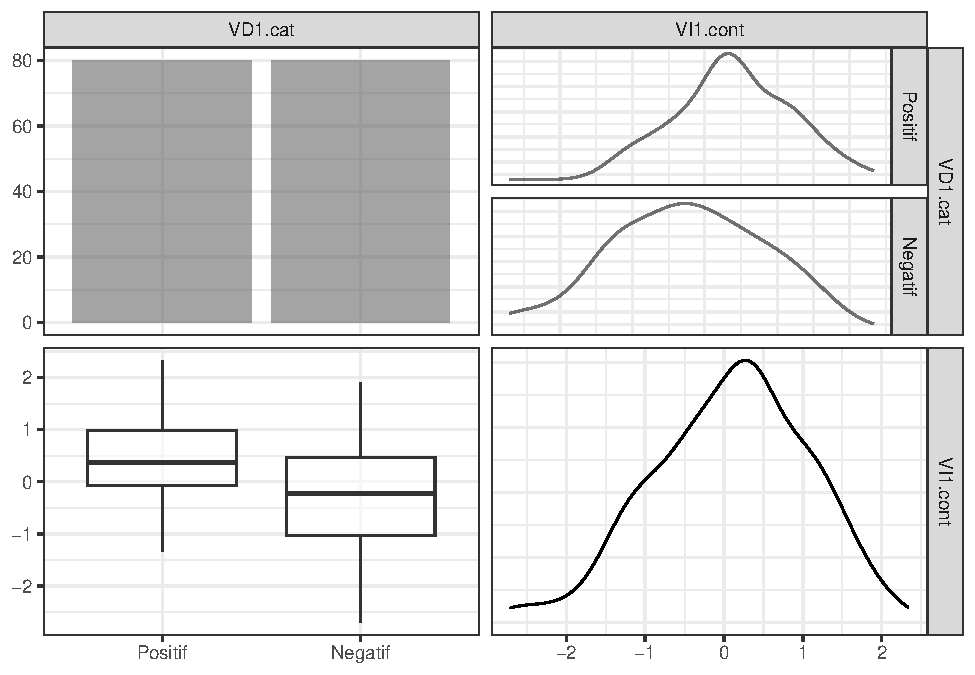
\includegraphics{Manuel_R_independant_files/figure-latex/unnamed-chunk-76-1.pdf}

\hypertarget{analyse-des-donnuxe9es-8}{%
\subsubsection{Analyse des données}\label{analyse-des-donnuxe9es-8}}

\begin{Shaded}
\begin{Highlighting}[]
\CommentTok{# calcul de la régression logistique binaire et stockage des résultats dans l’objet reglog.test}
\NormalTok{reglog.test <-}\StringTok{ }\KeywordTok{glm}\NormalTok{(}\DataTypeTok{formula =}\NormalTok{ VD1.cat }\OperatorTok{~}\StringTok{ }\NormalTok{VI1.cont, }
                   \DataTypeTok{family=} \StringTok{"binomial"}\NormalTok{, }
                   \DataTypeTok{data =}\NormalTok{ my_data.reglog)}

\CommentTok{# calcul de la taille d'effet de VD1.cont sur VI1.cat (odds ratio)}
\NormalTok{odds.ratio.reglog <-}\StringTok{ }\KeywordTok{exp}\NormalTok{(}\KeywordTok{coef}\NormalTok{(reglog.test))[}\DecValTok{2}\NormalTok{]}

\CommentTok{# obtention des résultats de la régression logistique binaire}
\KeywordTok{summary}\NormalTok{(reglog.test)}
\end{Highlighting}
\end{Shaded}

\begin{verbatim}
## 
## Call:
## glm(formula = VD1.cat ~ VI1.cont, family = "binomial", data = my_data.reglog)
## 
## Deviance Residuals: 
##      Min        1Q    Median        3Q       Max  
## -1.64933  -1.08682  -0.05088   1.07827   1.77801  
## 
## Coefficients:
##             Estimate Std. Error z value Pr(>|z|)    
## (Intercept)  0.06646    0.16855   0.394    0.693    
## VI1.cont    -0.74510    0.18973  -3.927  8.6e-05 ***
## ---
## Signif. codes:  0 '***' 0.001 '**' 0.01 '*' 0.05 '.' 0.1 ' ' 1
## 
## (Dispersion parameter for binomial family taken to be 1)
## 
##     Null deviance: 221.81  on 159  degrees of freedom
## Residual deviance: 203.78  on 158  degrees of freedom
## AIC: 207.78
## 
## Number of Fisher Scoring iterations: 4
\end{verbatim}

\begin{Shaded}
\begin{Highlighting}[]
\CommentTok{# obtention de la taille d'effet}
\NormalTok{odds.ratio.reglog}
\end{Highlighting}
\end{Shaded}

\begin{verbatim}
##  VI1.cont 
## 0.4746863
\end{verbatim}

\hypertarget{graphique-8}

\NormalTok{crude.slope.reglog <-}\StringTok{ }\KeywordTok{as.data.frame}\NormalTok{(}
  \KeywordTok{effect}\NormalTok{(}
    \DataTypeTok{term =} \StringTok{"VI1.cont"}\NormalTok{, }
    \DataTypeTok{mod =}\NormalTok{ reglog.test, }
    \DataTypeTok{data =}\NormalTok{ my_data.reglog))}

\KeywordTok{ggplot}\NormalTok{() }\OperatorTok{+}\StringTok{ }
\StringTok{  }\KeywordTok{geom_ribbon}\NormalTok{(}\DataTypeTok{data=}\NormalTok{crude.slope.reglog, }
              \KeywordTok{aes}\NormalTok{(}\DataTypeTok{x=}\NormalTok{VI1.cont, }\DataTypeTok{y=}\NormalTok{fit, }\DataTypeTok{ymin=}\NormalTok{lower, }\DataTypeTok{ymax=}\NormalTok{upper), }\DataTypeTok{fill=}\StringTok{"grey"}\NormalTok{, }\DataTypeTok{alpha=}\FloatTok{0.8}\NormalTok{) }\OperatorTok{+}\StringTok{ }
\StringTok{  }\KeywordTok{geom_line}\NormalTok{(}\DataTypeTok{data=}\NormalTok{crude.slope.reglog, }
            \KeywordTok{aes}\NormalTok{(}\DataTypeTok{x=}\NormalTok{VI1.cont, }\DataTypeTok{y=}\NormalTok{fit)) }\OperatorTok{+}\StringTok{ }
\StringTok{  }\KeywordTok{ylab}\NormalTok{(}\StringTok{"Probabilité que VD1.cat soit négatif"}\NormalTok{) }\OperatorTok{+}\StringTok{ }\KeywordTok{xlab}\NormalTok{(}\StringTok{"VI1.cont"}\NormalTok{) }\OperatorTok{+}
\StringTok{  }\KeywordTok{theme_bw}\NormalTok{() }\OperatorTok{+}\StringTok{ }
\StringTok{  }\KeywordTok{theme}\NormalTok{(}\DataTypeTok{axis.title.y =} \KeywordTok{element_text}\NormalTok{(}\DataTypeTok{size =} \DecValTok{14}\NormalTok{, }\DataTypeTok{hjust =} \FloatTok{0.5}\NormalTok{, }\DataTypeTok{face=}\StringTok{"bold"}\NormalTok{), }
        \DataTypeTok{axis.title.x =} \KeywordTok{element_text}\NormalTok{(}\DataTypeTok{face=}\StringTok{"bold"}\NormalTok{, }\DataTypeTok{size =} \DecValTok{14}\NormalTok{, }\DataTypeTok{hjust =} \FloatTok{0.5}\NormalTok{))}
\end{Highlighting}
\end{Shaded}

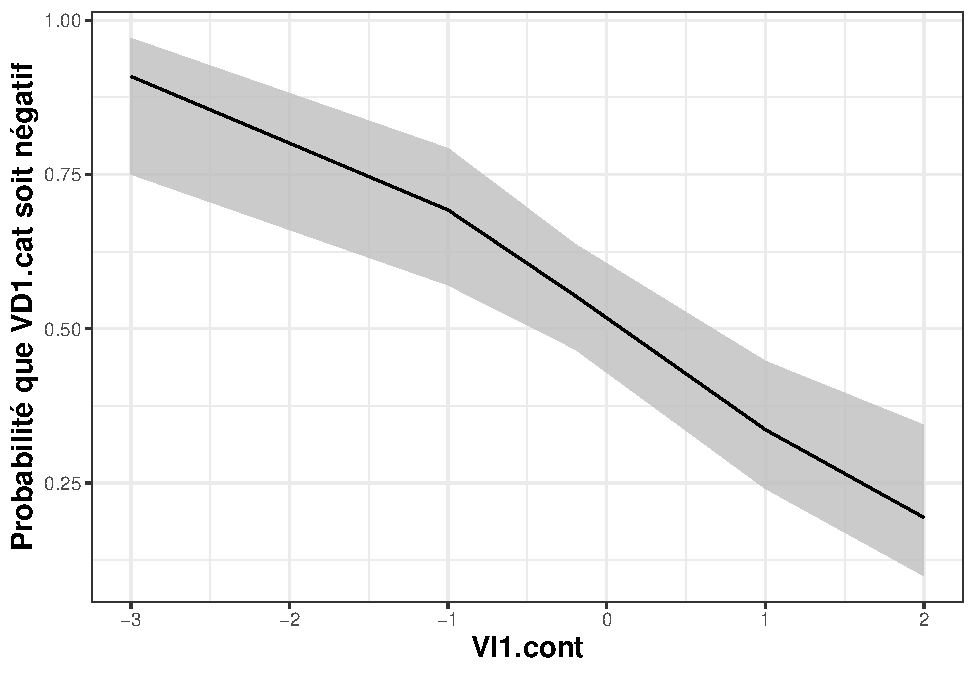
\includegraphics{Manuel_R_independant_files/figure-latex/unnamed-chunk-78-1.pdf}

\hypertarget{interpretation-8}{%
\subsubsection{Interpretation}\label{interpretation-8}}

{[}1{]} ``Les valeurs de VI1.cont sont liées à celles de VD1.cat: plus la valeur de VI1.cont est élevée, plus la probabilité que VD1.cat soit négatif est faible (b = -0.745, SE = 0.19, Odds Ratio = 0.475, p = 8.6e-05)''

\hypertarget{ruxe9gression-logistique-binaire-multiple-1}{%
\subsection{Régression logistique binaire multiple 1}\label{ruxe9gression-logistique-binaire-multiple-1}}

\hypertarget{type-de-variables-9}{%
\subsubsection{Type de variables}\label{type-de-variables-9}}

\textbf{Variable Dépendante :} Catégorielle (2 catégories)
\textbf{Variables Indépendantes :} Catégorielles (2 catégories ou +)

\hypertarget{packages-nuxe9cessaires-9}{%
\subsubsection{Packages nécessaires}\label{packages-nuxe9cessaires-9}}

\begin{Shaded}
\begin{Highlighting}[]
\KeywordTok{library}\NormalTok{(ggplot2)}
\KeywordTok{library}\NormalTok{(GGally)}
\KeywordTok{library}\NormalTok{(forcats)}
\KeywordTok{library}\NormalTok{(dplyr)}
\KeywordTok{library}\NormalTok{(car)}
\KeywordTok{library}\NormalTok{(emmeans)}
\end{Highlighting}
\end{Shaded}

\hypertarget{donnuxe9es-ruxe9elles-9}{%
\subsubsection{Données réelles}\label{donnuxe9es-ruxe9elles-9}}

\begin{Shaded}
\begin{Highlighting}[]
\CommentTok{# choisissez la ligne appropriée au format de votre fichier de données. }

\CommentTok{# si vos données sont dans un fichier .txt}
\NormalTok{my_data.reglog.mult1 <-}\StringTok{ }\KeywordTok{read.delim}\NormalTok{(}\KeywordTok{file.choose}\NormalTok{())}

\CommentTok{# si vos données sont dans un fichier .csv}
\NormalTok{my_data.reglog.mult1 <-}\StringTok{ }\KeywordTok{read.csv}\NormalTok{(}\KeywordTok{file.choose}\NormalTok{())}

\CommentTok{# si vos données sont dans un fichier .xls / .xlsx}
\NormalTok{my_data.reglog.mult1 <-}\StringTok{ }\KeywordTok{read_excel}\NormalTok{(}\KeywordTok{file.choose}\NormalTok{())}

\CommentTok{# une fois vos données chargées, vous pouvez renommer vos noms de colonnes afin qu'ils correspondent à ceux utilisés dans le code ci-dessous}
\CommentTok{# Si vous ne souhaitez pas renommer vos noms de colonnes, sautez cette étape mais adaptez le code des parties suivantes en lui indiquant les noms de colonnes de vos données.}

\CommentTok{# On crée une nouvelle colonne pour votre variable dépendante catégorielle (remplacez 'votre.nom.de.colonne' par le nom approprié)}
\NormalTok{my_data.reglog.mult1}\OperatorTok{$}\NormalTok{VD1.cat <-}\StringTok{ }\NormalTok{my_data.reglog.mult1}\OperatorTok{$}\StringTok{'votre.nom.de.colonne'}

\CommentTok{# On crée une nouvelle colonne pour vos variables indépendantes catégorielles(remplacez 'votre.nom.de.colonne' par les noms appropriés)}
\NormalTok{my_data.reglog.mult1}\OperatorTok{$}\NormalTok{VI1.cat <-}\StringTok{ }\NormalTok{my_data.reglog.mult1}\OperatorTok{$}\StringTok{'votre.nom.de.colonne'}
\NormalTok{my_data.reglog.mult1}\OperatorTok{$}\NormalTok{VI2.cat <-}\StringTok{ }\NormalTok{my_data.reglog.mult1}\OperatorTok{$}\StringTok{'votre.nom.de.colonne'}
\end{Highlighting}
\end{Shaded}

\hypertarget{donnuxe9es-fictives-9}{%
\subsubsection{Données fictives}\label{donnuxe9es-fictives-9}}

\begin{Shaded}
\begin{Highlighting}[]
\KeywordTok{set.seed}\NormalTok{(}\DecValTok{4321}\NormalTok{)}
\NormalTok{my_data.reglog.mult1 <-}\StringTok{ }\KeywordTok{data.frame}\NormalTok{(}
  \DataTypeTok{VD1.cat =} \KeywordTok{rbinom}\NormalTok{(}\DecValTok{200}\NormalTok{, }\DecValTok{1}\NormalTok{, }\FloatTok{0.5}\NormalTok{) }\OperatorTok{+}\StringTok{ }\DecValTok{1}\NormalTok{,}
  \DataTypeTok{VI1.cat =} \KeywordTok{rbinom}\NormalTok{(}\DecValTok{200}\NormalTok{, }\DecValTok{1}\NormalTok{, }\FloatTok{0.3}\NormalTok{) }\OperatorTok{+}\StringTok{ }\DecValTok{1}\NormalTok{,}
  \DataTypeTok{VI2.cat =} \KeywordTok{rbinom}\NormalTok{(}\DecValTok{200}\NormalTok{, }\DecValTok{1}\NormalTok{, }\FloatTok{0.3}\NormalTok{) }\OperatorTok{+}\StringTok{ }\DecValTok{1}\NormalTok{)}

\CommentTok{# On renomme les catégories de VD1.cat, VI1.cat et VI2.cat pour que les résultats soient plus lisibles}
\NormalTok{my_data.reglog.mult1}\OperatorTok{$}\NormalTok{VD1.cat <-}\StringTok{ }\KeywordTok{fct_recode}\NormalTok{(}\KeywordTok{factor}\NormalTok{(my_data.reglog.mult1}\OperatorTok{$}\NormalTok{VD1.cat), }
                                    \StringTok{"Positif"}\NormalTok{ =}\StringTok{ "1"}\NormalTok{, }
                                    \StringTok{"Negatif"}\NormalTok{ =}\StringTok{ "2"}\NormalTok{) }
\NormalTok{my_data.reglog.mult1}\OperatorTok{$}\NormalTok{VI1.cat <-}\StringTok{ }\KeywordTok{fct_recode}\NormalTok{(}\KeywordTok{factor}\NormalTok{(my_data.reglog.mult1}\OperatorTok{$}\NormalTok{VI1.cat), }
                                    \StringTok{"Groupe 1"}\NormalTok{ =}\StringTok{ "1"}\NormalTok{, }
                                    \StringTok{"Groupe 2"}\NormalTok{ =}\StringTok{ "2"}\NormalTok{) }
\NormalTok{my_data.reglog.mult1}\OperatorTok{$}\NormalTok{VI2.cat <-}\StringTok{ }\KeywordTok{fct_recode}\NormalTok{(}\KeywordTok{factor}\NormalTok{(my_data.reglog.mult1}\OperatorTok{$}\NormalTok{VI2.cat), }
                                    \StringTok{"Modalite 1"}\NormalTok{ =}\StringTok{ "1"}\NormalTok{, }
                                    \StringTok{"Modalite 2"}\NormalTok{ =}\StringTok{ "2"}\NormalTok{) }
\end{Highlighting}
\end{Shaded}

\hypertarget{duxe9claration-du-type-de-variables-8}{%
\subsubsection{Déclaration du type de variables}\label{duxe9claration-du-type-de-variables-8}}

\begin{Shaded}
\begin{Highlighting}[]
\NormalTok{my_data.reglog.mult1}\OperatorTok{$}\NormalTok{VD1.cat <-}\StringTok{ }\KeywordTok{factor}\NormalTok{(my_data.reglog.mult1}\OperatorTok{$}\NormalTok{VD1.cat)}
\NormalTok{my_data.reglog.mult1}\OperatorTok{$}\NormalTok{VI1.cat <-}\StringTok{ }\KeywordTok{factor}\NormalTok{(my_data.reglog.mult1}\OperatorTok{$}\NormalTok{VI1.cat)}
\NormalTok{my_data.reglog.mult1}\OperatorTok{$}\NormalTok{VI2.cat <-}\StringTok{ }\KeywordTok{factor}\NormalTok{(my_data.reglog.mult1}\OperatorTok{$}\NormalTok{VI2.cat)}
\end{Highlighting}
\end{Shaded}

\hypertarget{inspection-des-donnuxe9es-8}{%
\subsubsection{Inspection des données}\label{inspection-des-donnuxe9es-8}}

\begin{Shaded}
\begin{Highlighting}[]
\CommentTok{## Les graphiques situés sur la diagonale représentent la distribution des variables}
\CommentTok{## Les graphiques (ou les valeurs de corrélation) situés au dessus et en dessous de la diagonale représentent l'association entre les différentes variables}
\KeywordTok{ggpairs}\NormalTok{(my_data.reglog.mult1,}
        \DataTypeTok{lower =} \KeywordTok{list}\NormalTok{(}\DataTypeTok{continuous =} \KeywordTok{wrap}\NormalTok{(}\StringTok{"smooth"}\NormalTok{, }\DataTypeTok{alpha =} \FloatTok{0.7}\NormalTok{), }\DataTypeTok{combo =} \StringTok{"box_no_facet"}\NormalTok{),}
        \DataTypeTok{upper =} \KeywordTok{list}\NormalTok{(}\DataTypeTok{combo =} \StringTok{"facetdensity"}\NormalTok{, }\DataTypeTok{discrete =} \StringTok{"facetbar"}\NormalTok{), }
        \DataTypeTok{mapping =} \KeywordTok{aes}\NormalTok{(}\DataTypeTok{alpha =} \FloatTok{0.8}\NormalTok{)) }\OperatorTok{+}\StringTok{ }\KeywordTok{theme_bw}\NormalTok{()}
\end{Highlighting}
\end{Shaded}

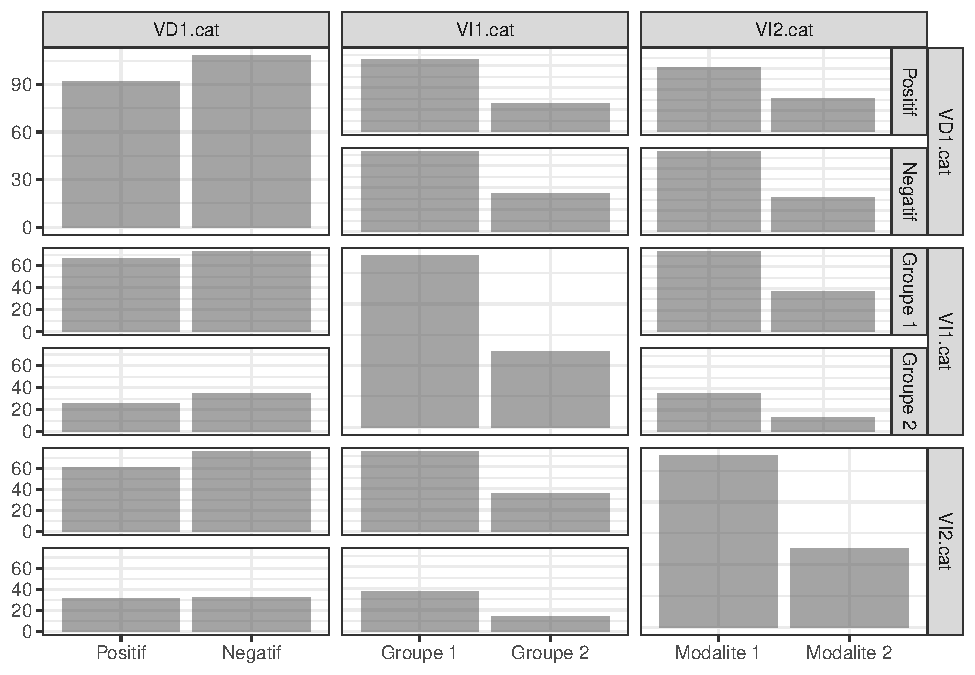
\includegraphics{Manuel_R_independant_files/figure-latex/unnamed-chunk-84-1.pdf}

\hypertarget{analyse-des-donnuxe9es-9}{%
\subsubsection{Analyse des données}\label{analyse-des-donnuxe9es-9}}

\begin{Shaded}
\begin{Highlighting}[]
\CommentTok{# calcul du test de régression logistique et stockage des résultats dans l’objet reglog.mult1.test}
\NormalTok{reglog.mult1.test <-}\StringTok{ }\KeywordTok{glm}\NormalTok{(}\DataTypeTok{formula =}\NormalTok{ VD1.cat }\OperatorTok{~}\StringTok{ }\NormalTok{VI1.cat}\OperatorTok{*}\NormalTok{VI2.cat, }
                    \DataTypeTok{family =} \StringTok{"binomial"}\NormalTok{, }
                    \DataTypeTok{contrasts =} \KeywordTok{list}\NormalTok{(}
                      \DataTypeTok{VI1.cat =} \StringTok{"contr.sum"}\NormalTok{, }
                      \DataTypeTok{VI2.cat =} \StringTok{"contr.sum"}\NormalTok{),}
                    \DataTypeTok{data =}\NormalTok{ my_data.reglog.mult1)}

\CommentTok{# calcul des proportions de VD1.cat dans chaque modalité de VI1.cat et VI2.cat}
\NormalTok{description.reglog.mult1 <-}\StringTok{ }\NormalTok{my_data.reglog.mult1 }\OperatorTok\StringTok{ }
\StringTok{    }\KeywordTok{group_by}\NormalTok{(VI1.cat, VI2.cat, VD1.cat) }\OperatorTok
\StringTok{    }\KeywordTok{summarise}\NormalTok{(}\DataTypeTok{N=}\KeywordTok{n}\NormalTok{()) }\OperatorTok
\StringTok{    }\KeywordTok{mutate}\NormalTok{(}\DataTypeTok{proportion =}\NormalTok{ N }\OperatorTok{/}\StringTok{ }\KeywordTok{sum}\NormalTok{(N))}

\CommentTok{# calcul de la taille d'effet de VI1.cat sur VD1.cat au sein de chaque modalité de VI2.cat (odds ratio)}
\NormalTok{posthoc.reglog.mult1 <-}\StringTok{ }\KeywordTok{emmeans}\NormalTok{(reglog.mult1.test, consec }\OperatorTok{~}\StringTok{ }\NormalTok{VI1.cat }\OperatorTok{|}\StringTok{ }\NormalTok{VI2.cat, }\DataTypeTok{type=}\StringTok{"response"}\NormalTok{)}

\CommentTok{# obtention des proportions  }
\NormalTok{description.reglog.mult1}
\end{Highlighting}
\end{Shaded}

\begin{verbatim}
## # A tibble: 8 x 5
## # Groups:   VI1.cat, VI2.cat [4]
##   VI1.cat  VI2.cat    VD1.cat     N proportion
##   <fct>    <fct>      <fct>   <int>      <dbl>
## 1 Groupe 1 Modalite 1 Positif    41      0.441
## 2 Groupe 1 Modalite 1 Negatif    52      0.559
## 3 Groupe 1 Modalite 2 Positif    25      0.543
## 4 Groupe 1 Modalite 2 Negatif    21      0.457
## 5 Groupe 2 Modalite 1 Positif    20      0.455
## 6 Groupe 2 Modalite 1 Negatif    24      0.545
## 7 Groupe 2 Modalite 2 Positif     6      0.353
## 8 Groupe 2 Modalite 2 Negatif    11      0.647
\end{verbatim}

\begin{Shaded}
\begin{Highlighting}[]
\CommentTok{# obtention des résultats de la régression logistique binaire multiple }
\KeywordTok{Anova}\NormalTok{(reglog.mult1.test, }\DataTypeTok{type =} \DecValTok{3}\NormalTok{)}
\end{Highlighting}
\end{Shaded}

\begin{verbatim}
## Analysis of Deviance Table (Type III tests)
## 
## Response: VD1.cat
##                 LR Chisq Df Pr(>Chisq)
## VI1.cat          1.11427  1     0.2912
## VI2.cat          0.00029  1     0.9864
## VI1.cat:VI2.cat  1.48152  1     0.2235
\end{verbatim}

\begin{Shaded}
\begin{Highlighting}[]
\CommentTok{# obtention des tailles d'effet (odds ratio)}
\CommentTok{# modalite 1}
\KeywordTok{summary}\NormalTok{(posthoc.reglog.mult1)}\OperatorTok{$}\NormalTok{contrasts}\OperatorTok{$}\NormalTok{odds.ratio[}\DecValTok{1}\NormalTok{]}
\end{Highlighting}
\end{Shaded}

\begin{verbatim}
## [1] 0.9461538
\end{verbatim}

\begin{Shaded}
\begin{Highlighting}[]
\CommentTok{# modalite 2}
\KeywordTok{summary}\NormalTok{(posthoc.reglog.mult1)}\OperatorTok{$}\NormalTok{contrasts}\OperatorTok{$}\NormalTok{odds.ratio[}\DecValTok{2}\NormalTok{]}
\end{Highlighting}
\end{Shaded}

\begin{verbatim}
## [1] 2.18254
\end{verbatim}

\hypertarget{graphique-9}{%
\subsubsection{Graphique}\label{graphique-9}}

\begin{Shaded}
\begin{Highlighting}[]
\KeywordTok{ggplot}\NormalTok{(}\KeywordTok{subset}\NormalTok{(description.reglog.mult1, VD1.cat }\OperatorTok{==}\StringTok{ "Positif"}\NormalTok{), }
       \KeywordTok{aes}\NormalTok{(}\DataTypeTok{x =}\NormalTok{ VI1.cat, }\DataTypeTok{y =}\NormalTok{ proportion, }\DataTypeTok{fill =}\NormalTok{ VI1.cat)) }\OperatorTok{+}\StringTok{ }
\StringTok{  }\KeywordTok{geom_bar}\NormalTok{(}\DataTypeTok{stat =} \StringTok{"identity"}\NormalTok{, }\DataTypeTok{position=}\KeywordTok{position_dodge2}\NormalTok{()) }\OperatorTok{+}\StringTok{ }
\StringTok{  }\KeywordTok{facet_wrap}\NormalTok{(}\OperatorTok{~}\NormalTok{VI2.cat) }\OperatorTok{+}\StringTok{ }
\StringTok{  }\KeywordTok{scale_fill_grey}\NormalTok{(}\DataTypeTok{start =} \FloatTok{0.8}\NormalTok{, }\DataTypeTok{end =} \FloatTok{0.5}\NormalTok{) }\OperatorTok{+}
\StringTok{  }\KeywordTok{ylab}\NormalTok{(}\StringTok{"Proportion de personnes ayant}\CharTok{\textbackslash{}n}\StringTok{ un score positif"}\NormalTok{) }\OperatorTok{+}\StringTok{ }\KeywordTok{xlab}\NormalTok{(}\StringTok{"VI1.cat"}\NormalTok{) }\OperatorTok{+}\StringTok{ }
\StringTok{  }\KeywordTok{theme_bw}\NormalTok{() }\OperatorTok{+}\StringTok{ }
\StringTok{  }\KeywordTok{theme}\NormalTok{(}\DataTypeTok{axis.title.y =} \KeywordTok{element_text}\NormalTok{(}\DataTypeTok{size =} \DecValTok{14}\NormalTok{, }\DataTypeTok{hjust =} \FloatTok{0.5}\NormalTok{, }\DataTypeTok{face =} \StringTok{"bold"}\NormalTok{), }
        \DataTypeTok{axis.title.x =} \KeywordTok{element_text}\NormalTok{(}\DataTypeTok{face =} \StringTok{"bold"}\NormalTok{, }\DataTypeTok{size =} \DecValTok{14}\NormalTok{, }\DataTypeTok{hjust =} \FloatTok{0.5}\NormalTok{)) }\OperatorTok{+}
\StringTok{  }\KeywordTok{guides}\NormalTok{(}\DataTypeTok{fill =} \OtherTok{FALSE}\NormalTok{)}
\end{Highlighting}
\end{Shaded}

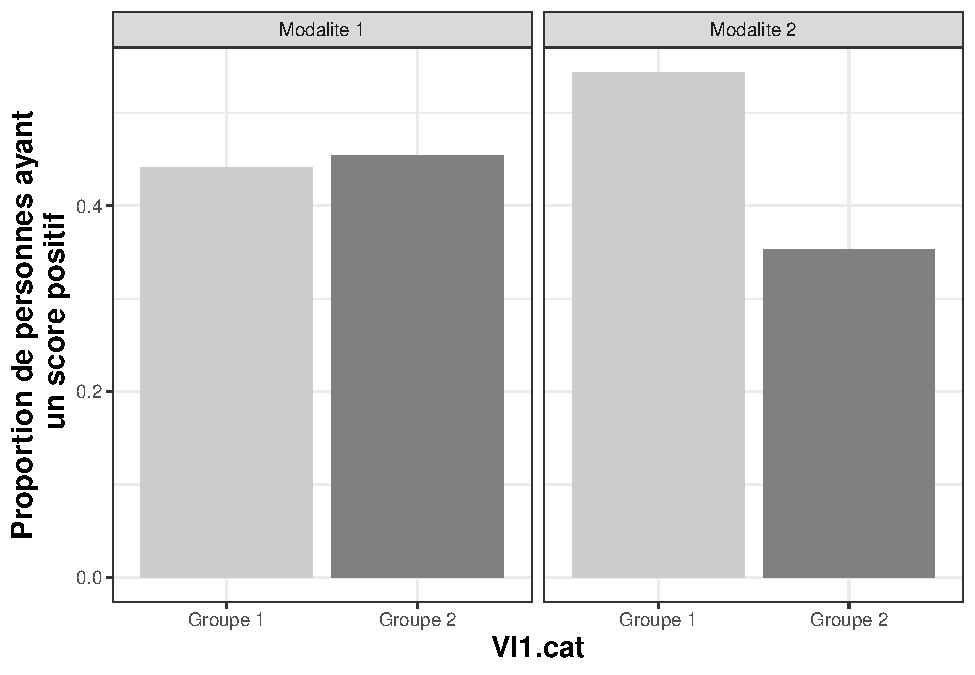
\includegraphics{Manuel_R_independant_files/figure-latex/unnamed-chunk-86-1.pdf}

\hypertarget{interpretation-9}{%
\subsubsection{Interpretation}\label{interpretation-9}}

{[}1{]} ``La différence de proportion de cas positifs entre les groupes ne diffère pas statistiquement entre la modalité 1 (groupe 1 = 44.1\%, groupe 2 = 45.5\%, Odds Ratio = 0.946) et la modalité 2 de VI2.cat (groupe 2 = 54.3\%, groupe 2 = 35.3\%, Odds Ratio = 2.183; X² = 1.482, p = 0.224)''

\hypertarget{ruxe9gression-logistique-binaire-multiple-2}{%
\subsection{Régression logistique binaire multiple 2}\label{ruxe9gression-logistique-binaire-multiple-2}}

\hypertarget{type-de-variables-10}{%
\subsubsection{Type de variables}\label{type-de-variables-10}}

\textbf{Variable Dépendante :} Catégorielle (2 catégories)
\textbf{Variables Indépendantes :} Numériques

\hypertarget{packages-nuxe9cessaires-10}{%
\subsubsection{Packages nécessaires}\label{packages-nuxe9cessaires-10}}

\begin{Shaded}
\begin{Highlighting}[]
\KeywordTok{library}\NormalTok{(ggplot2)}
\KeywordTok{library}\NormalTok{(GGally)}
\KeywordTok{library}\NormalTok{(forcats)}
\KeywordTok{library}\NormalTok{(effects)}
\end{Highlighting}
\end{Shaded}

\hypertarget{donnuxe9es-ruxe9elles-10}{%
\subsubsection{Données réelles}\label{donnuxe9es-ruxe9elles-10}}

\begin{Shaded}
\begin{Highlighting}[]
\CommentTok{# choisissez la ligne appropriée au format de votre fichier de données. }

\CommentTok{# si vos données sont dans un fichier .txt}
\NormalTok{my_data.reglog.mult2 <-}\StringTok{ }\KeywordTok{read.delim}\NormalTok{(}\KeywordTok{file.choose}\NormalTok{())}

\CommentTok{# si vos données sont dans un fichier .csv}
\NormalTok{my_data.reglog.mult2 <-}\StringTok{ }\KeywordTok{read.csv}\NormalTok{(}\KeywordTok{file.choose}\NormalTok{())}

\CommentTok{# si vos données sont dans un fichier .xls / .xlsx}
\NormalTok{my_data.reglog.mult2 <-}\StringTok{ }\KeywordTok{read_excel}\NormalTok{(}\KeywordTok{file.choose}\NormalTok{())}

\CommentTok{# une fois vos données chargées, vous pouvez renommer vos noms de colonnes afin qu'ils correspondent à ceux utilisés dans le code ci-dessous}
\CommentTok{# Si vous ne souhaitez pas renommer vos noms de colonnes, sautez cette étape mais adaptez le code des parties suivantes en lui indiquant les noms de colonnes de vos données.}

\CommentTok{# On crée une nouvelle colonne pour votre variable dépendante catégorielle (remplacez 'votre.nom.de.colonne' par le nom approprié)}
\NormalTok{my_data.reglog.mult2}\OperatorTok{$}\NormalTok{VD1.cat <-}\StringTok{ }\NormalTok{my_data.reglog.mult2}\OperatorTok{$}\StringTok{'votre.nom.de.colonne'}

\CommentTok{# On crée une nouvelle colonne pour votre variable indépendante continue (remplacez 'votre.nom.de.colonne' par le nom approprié)}
\NormalTok{my_data.reglog.mult2}\OperatorTok{$}\NormalTok{VI1.cont <-}\StringTok{ }\NormalTok{my_data.reglog.mult2}\OperatorTok{$}\StringTok{'votre.nom.de.colonne'}
\end{Highlighting}
\end{Shaded}

\hypertarget{donnuxe9es-fictives-10}{%
\subsubsection{Données fictives}\label{donnuxe9es-fictives-10}}

\begin{Shaded}
\begin{Highlighting}[]
\KeywordTok{set.seed}\NormalTok{(}\DecValTok{4321}\NormalTok{)}
\NormalTok{my_data.reglog.mult2 <-}\StringTok{ }\KeywordTok{data.frame}\NormalTok{(}
  \DataTypeTok{VD1.cat =} \KeywordTok{rbinom}\NormalTok{(}\DecValTok{25}\NormalTok{, }\DecValTok{1}\NormalTok{, }\FloatTok{0.7}\NormalTok{) }\OperatorTok{+}\StringTok{ }\DecValTok{1}\NormalTok{,}
  \DataTypeTok{VI1.cont =} \KeywordTok{rnorm}\NormalTok{(}\DecValTok{25}\NormalTok{),}
  \DataTypeTok{VI2.cont =} \KeywordTok{rnorm}\NormalTok{(}\DecValTok{25}\NormalTok{))}

\CommentTok{# on renomme les catégories de VD1.cat pour que les résultats soient plus lisibles}
\NormalTok{my_data.reglog.mult2}\OperatorTok{$}\NormalTok{VD1.cat <-}\StringTok{ }\KeywordTok{fct_recode}\NormalTok{(}\KeywordTok{factor}\NormalTok{(my_data.reglog.mult2}\OperatorTok{$}\NormalTok{VD1.cat), }
                                           \StringTok{"Positif"}\NormalTok{ =}\StringTok{ "1"}\NormalTok{, }
                                           \StringTok{"Negatif"}\NormalTok{ =}\StringTok{ "2"}\NormalTok{) }
\end{Highlighting}
\end{Shaded}

\hypertarget{duxe9claration-du-type-de-variables-9}{%
\subsubsection{Déclaration du type de variables}\label{duxe9claration-du-type-de-variables-9}}

\begin{Shaded}
\begin{Highlighting}[]
\NormalTok{my_data.reglog.mult2}\OperatorTok{$}\NormalTok{VD1.cat <-}\StringTok{ }\KeywordTok{factor}\NormalTok{(my_data.reglog.mult2}\OperatorTok{$}\NormalTok{VD1.cat)}
\NormalTok{my_data.reglog.mult2}\OperatorTok{$}\NormalTok{VI1.cont <-}\StringTok{ }\KeywordTok{as.numeric}\NormalTok{(}\KeywordTok{as.character}\NormalTok{(my_data.reglog.mult2}\OperatorTok{$}\NormalTok{VI1.cont))}
\NormalTok{my_data.reglog.mult2}\OperatorTok{$}\NormalTok{VI2.cont <-}\StringTok{ }\KeywordTok{as.numeric}\NormalTok{(}\KeywordTok{as.character}\NormalTok{(my_data.reglog.mult2}\OperatorTok{$}\NormalTok{VI2.cont))}
\end{Highlighting}
\end{Shaded}

\hypertarget{inspection-des-donnuxe9es-9}{%
\subsubsection{Inspection des données}\label{inspection-des-donnuxe9es-9}}

\begin{Shaded}
\begin{Highlighting}[]
\CommentTok{## Les graphiques situés sur la diagonale représentent la distribution des variables}
\CommentTok{## Les graphiques (ou les valeurs de corrélation) situés au dessus et en dessous de la diagonale représentent l'association entre les différentes variables}
\KeywordTok{ggpairs}\NormalTok{(my_data.reglog.mult2,}
        \DataTypeTok{lower =} \KeywordTok{list}\NormalTok{(}\DataTypeTok{continuous =} \KeywordTok{wrap}\NormalTok{(}\StringTok{"smooth"}\NormalTok{, }\DataTypeTok{alpha =} \FloatTok{0.7}\NormalTok{), }\DataTypeTok{combo =} \StringTok{"box_no_facet"}\NormalTok{),}
        \DataTypeTok{upper =} \KeywordTok{list}\NormalTok{(}\DataTypeTok{combo =} \StringTok{"facetdensity"}\NormalTok{, }\DataTypeTok{discrete =} \StringTok{"facetbar"}\NormalTok{), }
        \DataTypeTok{mapping =} \KeywordTok{aes}\NormalTok{(}\DataTypeTok{alpha =} \FloatTok{0.8}\NormalTok{)) }\OperatorTok{+}\StringTok{ }\KeywordTok{theme_bw}\NormalTok{()}
\end{Highlighting}
\end{Shaded}

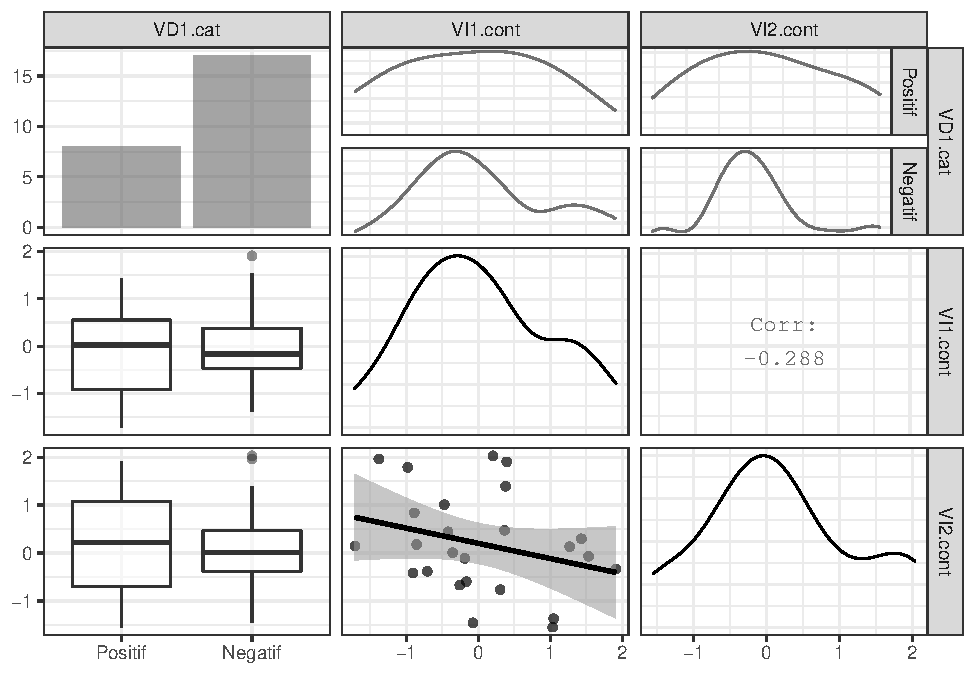
\includegraphics{Manuel_R_independant_files/figure-latex/unnamed-chunk-92-1.pdf}

\hypertarget{analyse-des-donnuxe9es-10}{%
\subsubsection{Analyse des données}\label{analyse-des-donnuxe9es-10}}

\begin{Shaded}
\begin{Highlighting}[]
\CommentTok{# calcul de la régression logistique binaire multiple et stockage des résultats dans l’objet reglog.mult2.test}
\NormalTok{reglog.mult2.test <-}\StringTok{ }\KeywordTok{glm}\NormalTok{(}\DataTypeTok{formula =}\NormalTok{ VD1.cat }\OperatorTok{~}\StringTok{ }\NormalTok{VI1.cont }\OperatorTok{+}\StringTok{ }\NormalTok{VI2.cont, }
                         \DataTypeTok{family=} \StringTok{"binomial"}\NormalTok{, }
                         \DataTypeTok{data =}\NormalTok{ my_data.reglog.mult2)}

\CommentTok{# calcul de la taille d'effet de VI1.cont sur VD1.cat (odds ratio ajusté par VI2.cont)}
\NormalTok{odds.ratio.reglog.mult2 <-}\StringTok{ }\KeywordTok{exp}\NormalTok{(}\KeywordTok{coef}\NormalTok{(reglog.mult2.test))[}\DecValTok{2}\NormalTok{]}

\CommentTok{# obtention  des résultats de la régression logistique binaire multiple}
\KeywordTok{summary}\NormalTok{(reglog.mult2.test)}
\end{Highlighting}
\end{Shaded}

\begin{verbatim}
## 
## Call:
## glm(formula = VD1.cat ~ VI1.cont + VI2.cont, family = "binomial", 
##     data = my_data.reglog.mult2)
## 
## Deviance Residuals: 
##     Min       1Q   Median       3Q      Max  
## -1.6190  -1.4139   0.8582   0.8977   0.9867  
## 
## Coefficients:
##             Estimate Std. Error z value Pr(>|z|)  
## (Intercept)  0.76151    0.44031   1.729   0.0837 .
## VI1.cont     0.17030    0.48817   0.349   0.7272  
## VI2.cont    -0.03048    0.43743  -0.070   0.9444  
## ---
## Signif. codes:  0 '***' 0.001 '**' 0.01 '*' 0.05 '.' 0.1 ' ' 1
## 
## (Dispersion parameter for binomial family taken to be 1)
## 
##     Null deviance: 31.343  on 24  degrees of freedom
## Residual deviance: 31.189  on 22  degrees of freedom
## AIC: 37.189
## 
## Number of Fisher Scoring iterations: 4
\end{verbatim}

\begin{Shaded}
\begin{Highlighting}[]
\CommentTok{# obtention de la taille d'effet}
\NormalTok{odds.ratio.reglog.mult2}
\end{Highlighting}
\end{Shaded}

\begin{verbatim}
## VI1.cont 
## 1.185656
\end{verbatim}

\hypertarget{graphique-10}
\NormalTok{adjusted.slope.reglog.mult2 <-}\StringTok{ }\KeywordTok{as.data.frame}\NormalTok{(}
  \KeywordTok{effect}\NormalTok{(}
    \DataTypeTok{term =} \StringTok{"VI1.cont"}\NormalTok{, }
    \DataTypeTok{mod =}\NormalTok{ reglog.mult2.test, }
    \DataTypeTok{data =}\NormalTok{ my_data.reglog.mult2))}

\KeywordTok{ggplot}\NormalTok{(adjusted.slope.reglog.mult2, }\KeywordTok{aes}\NormalTok{(}\DataTypeTok{x =}\NormalTok{ VI1.cont, }\DataTypeTok{y =}\NormalTok{ fit)) }\OperatorTok{+}\StringTok{ }
\StringTok{  }\KeywordTok{geom_ribbon}\NormalTok{( }\KeywordTok{aes}\NormalTok{(}\DataTypeTok{ymin =}\NormalTok{ lower, }\DataTypeTok{ymax =}\NormalTok{ upper), }\DataTypeTok{fill =} \StringTok{"grey"}\NormalTok{, }\DataTypeTok{alpha =} \FloatTok{0.8}\NormalTok{) }\OperatorTok{+}\StringTok{ }
\StringTok{  }\KeywordTok{geom_line}\NormalTok{() }\OperatorTok{+}\StringTok{ }
\StringTok{  }\KeywordTok{ylab}\NormalTok{(}\StringTok{"Probabilité que VD1.cat soit négatif"}\NormalTok{) }\OperatorTok{+}\StringTok{ }\KeywordTok{xlab}\NormalTok{(}\StringTok{"VI1.cont"}\NormalTok{) }\OperatorTok{+}
\StringTok{  }\KeywordTok{theme_bw}\NormalTok{() }\OperatorTok{+}\StringTok{ }
\StringTok{  }\KeywordTok{theme}\NormalTok{(}\DataTypeTok{axis.title.y =} \KeywordTok{element_text}\NormalTok{(}\DataTypeTok{size =} \DecValTok{14}\NormalTok{, }\DataTypeTok{hjust =} \FloatTok{0.5}\NormalTok{, }\DataTypeTok{face =} \StringTok{"bold"}\NormalTok{), }
        \DataTypeTok{axis.title.x =} \KeywordTok{element_text}\NormalTok{(}\DataTypeTok{face =} \StringTok{"bold"}\NormalTok{, }\DataTypeTok{size =} \DecValTok{14}\NormalTok{, }\DataTypeTok{hjust =} \FloatTok{0.5}\NormalTok{))}
\end{Highlighting}
\end{Shaded}

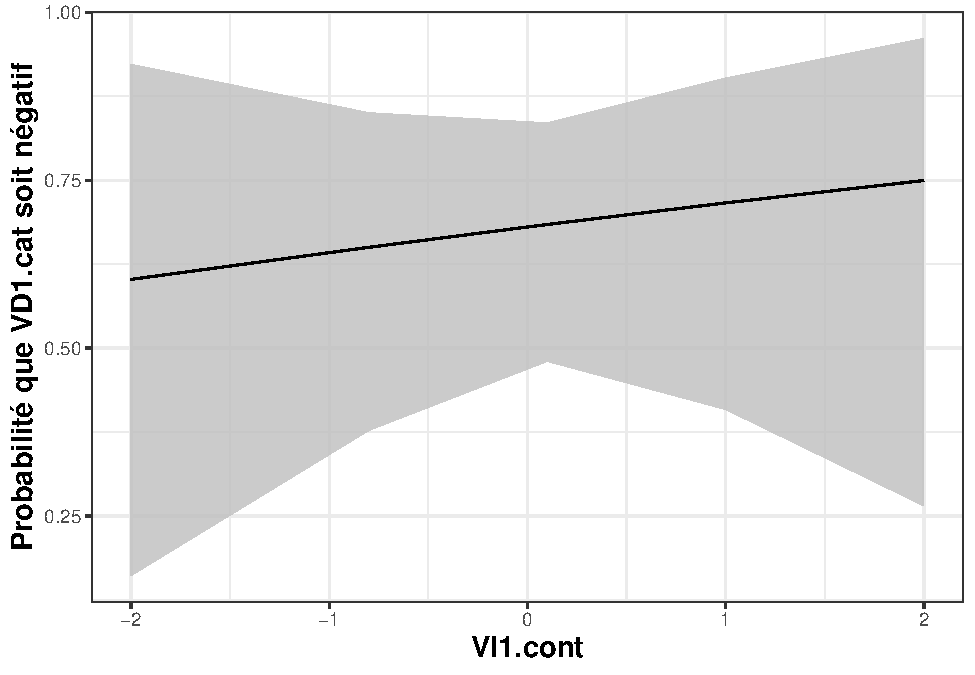
\includegraphics{Manuel_R_independant_files/figure-latex/unnamed-chunk-94-1.pdf}

\hypertarget{interpretation-10}{%
\subsubsection{Interpretation}\label{interpretation-10}}

{[}1{]} ``VI1.cont n'est pas lié à VD1.cat lorsque l'on ajuste par l'effet de VI2.cont (b = 0.17, SE = 0.488, Odds Ratio = 1.186, p = 0.727203)''

\hypertarget{ruxe9gression-logistique-binaire-multiple-3}{%
\subsection{Régression logistique binaire multiple 3}\label{ruxe9gression-logistique-binaire-multiple-3}}

\hypertarget{type-de-variables-11}{%
\subsubsection{Type de variables}\label{type-de-variables-11}}

\textbf{Variable Dépendante :} Catégorielle (2 catégories)
\textbf{Variables Indépendantes :} Numériques / Catégorielles

\hypertarget{packages-nuxe9cessaires-11}{%
\subsubsection{Packages nécessaires}\label{packages-nuxe9cessaires-11}}

\begin{Shaded}
\begin{Highlighting}[]
\KeywordTok{library}\NormalTok{(ggplot2)}
\KeywordTok{library}\NormalTok{(GGally)}
\KeywordTok{library}\NormalTok{(forcats)}
\KeywordTok{library}\NormalTok{(effects)}
\end{Highlighting}
\end{Shaded}

\hypertarget{donnuxe9es-ruxe9elles-11}{%
\subsubsection{Données réelles}\label{donnuxe9es-ruxe9elles-11}}

\begin{Shaded}
\begin{Highlighting}[]
\CommentTok{# choisissez la ligne appropriée au format de votre fichier de données. }

\CommentTok{# si vos données sont dans un fichier .txt}
\NormalTok{my_data.reglog.mult3 <-}\StringTok{ }\KeywordTok{read.delim}\NormalTok{(}\KeywordTok{file.choose}\NormalTok{())}

\CommentTok{# si vos données sont dans un fichier .csv}
\NormalTok{my_data.reglog.mult3 <-}\StringTok{ }\KeywordTok{read.csv}\NormalTok{(}\KeywordTok{file.choose}\NormalTok{())}

\CommentTok{# si vos données sont dans un fichier .xls / .xlsx}
\NormalTok{my_data.reglog.mult3 <-}\StringTok{ }\KeywordTok{read_excel}\NormalTok{(}\KeywordTok{file.choose}\NormalTok{())}

\CommentTok{# une fois vos données chargées, vous pouvez renommer vos noms de colonnes afin qu'ils correspondent à ceux utilisés dans le code ci-dessous}
\CommentTok{# Si vous ne souhaitez pas renommer vos noms de colonnes, sautez cette étape mais adaptez le code des parties suivantes en lui indiquant les noms de colonnes de vos données.}

\CommentTok{# On crée une nouvelle colonne pour votre variable dépendante continue (remplacez 'votre.nom.de.colonne' par le nom approprié)}
\NormalTok{my_data.reglog.mult3}\OperatorTok{$}\NormalTok{VD1.cat <-}\StringTok{ }\NormalTok{my_data.reglog.mult3}\OperatorTok{$}\StringTok{'votre.nom.de.colonne'}

\CommentTok{# On crée une nouvelle colonne pour vos variables indépendantes continues (remplacez 'votre.nom.de.colonne' par les noms appropriés)}
\NormalTok{my_data.reglog.mult3}\OperatorTok{$}\NormalTok{VI1.cont <-}\StringTok{ }\NormalTok{my_data.reglog.mult3}\OperatorTok{$}\StringTok{'votre.nom.de.colonne'}
\NormalTok{my_data.reglog.mult3}\OperatorTok{$}\NormalTok{VI3.cont <-}\StringTok{ }\NormalTok{my_data.reglog.mult3}\OperatorTok{$}\StringTok{'votre.nom.de.colonne'}

\CommentTok{# On crée une nouvelle colonne pour votre variable indépendante catégorielle (remplacez 'votre.nom.de.colonne' par le nom approprié)}
\NormalTok{my_data.reglog.mult3}\OperatorTok{$}\NormalTok{VI2.cat <-}\StringTok{ }\NormalTok{my_data.reglog.mult3}\OperatorTok{$}\StringTok{'votre.nom.de.colonne'}
\end{Highlighting}
\end{Shaded}

\hypertarget{donnuxe9es-fictives-11}{%
\subsubsection{Données fictives}\label{donnuxe9es-fictives-11}}

\begin{Shaded}
\begin{Highlighting}[]
\KeywordTok{set.seed}\NormalTok{(}\DecValTok{4321}\NormalTok{)}
\NormalTok{my_data.reglog.mult3 <-}\StringTok{ }\KeywordTok{data.frame}\NormalTok{(}
  \DataTypeTok{VD1.cat =} \KeywordTok{rep}\NormalTok{(}\KeywordTok{c}\NormalTok{(}\DecValTok{1}\NormalTok{,}\DecValTok{2}\NormalTok{), }\DataTypeTok{each =} \DecValTok{150}\NormalTok{),}
  \DataTypeTok{VI1.cont =} \KeywordTok{c}\NormalTok{(}\KeywordTok{rnorm}\NormalTok{(}\DecValTok{150}\NormalTok{) }\OperatorTok{+}\StringTok{ }\FloatTok{0.2}\NormalTok{, }\KeywordTok{rnorm}\NormalTok{(}\DecValTok{150}\NormalTok{) }\OperatorTok{-}\StringTok{ }\FloatTok{0.2}\NormalTok{),}
  \DataTypeTok{VI2.cat =} \KeywordTok{rbinom}\NormalTok{(}\DecValTok{300}\NormalTok{, }\DecValTok{1}\NormalTok{, }\FloatTok{0.4}\NormalTok{) }\OperatorTok{+}\StringTok{ }\DecValTok{1}\NormalTok{,}
  \DataTypeTok{VI3.cont =} \KeywordTok{rnorm}\NormalTok{(}\DecValTok{300}\NormalTok{))}

\CommentTok{# on renomme les catégories de VD1.cat et VI2.cat pour que les résultats soient plus lisibles}
\NormalTok{my_data.reglog.mult3}\OperatorTok{$}\NormalTok{VD1.cat <-}\StringTok{ }\KeywordTok{fct_recode}\NormalTok{(}\KeywordTok{factor}\NormalTok{(my_data.reglog.mult3}\OperatorTok{$}\NormalTok{VD1.cat), }
                                           \StringTok{"Positif"}\NormalTok{ =}\StringTok{ "1"}\NormalTok{, }
                                           \StringTok{"Negatif"}\NormalTok{ =}\StringTok{ "2"}\NormalTok{) }
\NormalTok{my_data.reglog.mult3}\OperatorTok{$}\NormalTok{VI2.cat <-}\StringTok{ }\KeywordTok{fct_recode}\NormalTok{(}\KeywordTok{factor}\NormalTok{(my_data.reglog.mult3}\OperatorTok{$}\NormalTok{VI2.cat), }
                                           \StringTok{"Modalite 1"}\NormalTok{ =}\StringTok{ "1"}\NormalTok{, }
                                           \StringTok{"Modalite 2"}\NormalTok{ =}\StringTok{ "2"}\NormalTok{) }
\end{Highlighting}
\end{Shaded}

\hypertarget{duxe9claration-du-type-de-variables-10}{%
\subsubsection{Déclaration du type de variables}\label{duxe9claration-du-type-de-variables-10}}

\begin{Shaded}
\begin{Highlighting}[]
\NormalTok{my_data.reglog.mult3}\OperatorTok{$}\NormalTok{VD1.cat <-}\StringTok{ }\KeywordTok{factor}\NormalTok{(my_data.reglog.mult3}\OperatorTok{$}\NormalTok{VD1.cat)}
\NormalTok{my_data.reglog.mult3}\OperatorTok{$}\NormalTok{VI1.cont <-}\StringTok{ }\KeywordTok{as.numeric}\NormalTok{(}\KeywordTok{as.character}\NormalTok{(my_data.reglog.mult3}\OperatorTok{$}\NormalTok{VI1.cont))}
\NormalTok{my_data.reglog.mult3}\OperatorTok{$}\NormalTok{VI2.cat <-}\StringTok{ }\KeywordTok{factor}\NormalTok{(my_data.reglog.mult3}\OperatorTok{$}\NormalTok{VI2.cat)}
\NormalTok{my_data.reglog.mult3}\OperatorTok{$}\NormalTok{VI3.cont <-}\StringTok{ }\KeywordTok{as.numeric}\NormalTok{(}\KeywordTok{as.character}\NormalTok{(my_data.reglog.mult3}\OperatorTok{$}\NormalTok{VI3.cont))}
\end{Highlighting}
\end{Shaded}

\hypertarget{inspection-des-donnuxe9es-10}{%
\subsubsection{Inspection des données}\label{inspection-des-donnuxe9es-10}}

\begin{Shaded}
\begin{Highlighting}[]
\CommentTok{## Les graphiques situés sur la diagonale représentent la distribution des variables}
\CommentTok{## Les graphiques (ou les valeurs de corrélation) situés au dessus et en dessous de la diagonale représentent l'association entre les différentes variables}
\KeywordTok{ggpairs}\NormalTok{(my_data.reglog.mult3,}
        \DataTypeTok{lower =} \KeywordTok{list}\NormalTok{(}\DataTypeTok{continuous =} \KeywordTok{wrap}\NormalTok{(}\StringTok{"smooth"}\NormalTok{, }\DataTypeTok{alpha =} \FloatTok{0.7}\NormalTok{), }\DataTypeTok{combo =} \StringTok{"box_no_facet"}\NormalTok{),}
        \DataTypeTok{upper =} \KeywordTok{list}\NormalTok{(}\DataTypeTok{combo =} \StringTok{"facetdensity"}\NormalTok{, }\DataTypeTok{discrete =} \StringTok{"facetbar"}\NormalTok{), }
        \DataTypeTok{mapping =} \KeywordTok{aes}\NormalTok{(}\DataTypeTok{alpha =} \FloatTok{0.8}\NormalTok{)) }\OperatorTok{+}\StringTok{ }\KeywordTok{theme_bw}\NormalTok{()}
\end{Highlighting}
\end{Shaded}

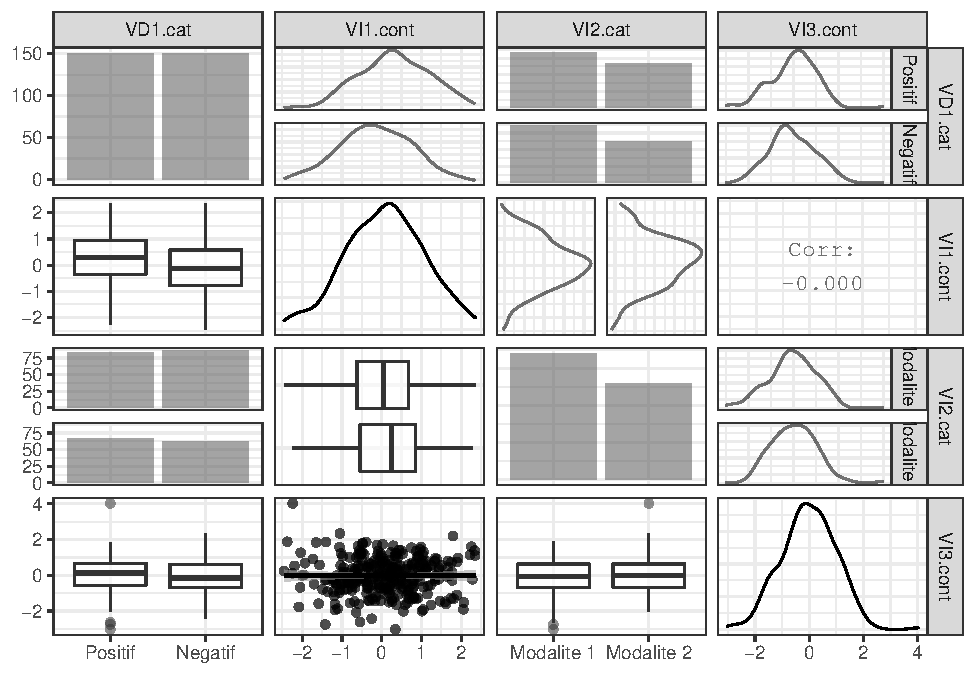
\includegraphics{Manuel_R_independant_files/figure-latex/unnamed-chunk-100-1.pdf}

\hypertarget{analyse-des-donnuxe9es-11}{%
\subsubsection{Analyse des données}\label{analyse-des-donnuxe9es-11}}

\begin{Shaded}
\begin{Highlighting}[]
\CommentTok{# calcul de la régression logistique binaire multiple et stockage des résultats dans l’objet reglog.mult3.test}
\NormalTok{reglog.mult3.test <-}\StringTok{ }\KeywordTok{glm}\NormalTok{(}\DataTypeTok{formula =}\NormalTok{ VD1.cat }\OperatorTok{~}\StringTok{ }\NormalTok{VI1.cont }\OperatorTok{+}\StringTok{ }\NormalTok{VI2.cat }\OperatorTok{+}\StringTok{ }\NormalTok{VI3.cont, }
                         \DataTypeTok{family=} \StringTok{"binomial"}\NormalTok{, }
                         \DataTypeTok{data =}\NormalTok{ my_data.reglog.mult3)}


\CommentTok{# calcul de la taille d'effet de VI1.cont sur VD1. cat (odds ratio ajusté par VI2.cat et VI3.cont)}
\NormalTok{odds.ratio.reglog.mult3 <-}\StringTok{ }\KeywordTok{exp}\NormalTok{(}\KeywordTok{coef}\NormalTok{(reglog.mult3.test))[}\DecValTok{2}\NormalTok{]}

\CommentTok{# obtention des résultats de la régression logistique binaire multiple}
\KeywordTok{summary}\NormalTok{(reglog.mult3.test)}
\end{Highlighting}
\end{Shaded}

\begin{verbatim}
## 
## Call:
## glm(formula = VD1.cat ~ VI1.cont + VI2.cat + VI3.cont, family = "binomial", 
##     data = my_data.reglog.mult3)
## 
## Deviance Residuals: 
##     Min       1Q   Median       3Q      Max  
## -1.6685  -1.1308  -0.0127   1.1321   1.6838  
## 
## Coefficients:
##                   Estimate Std. Error z value Pr(>|z|)    
## (Intercept)        0.05500    0.15752   0.349 0.726970    
## VI1.cont          -0.47028    0.12607  -3.730 0.000191 ***
## VI2.catModalite 2 -0.03680    0.23982  -0.153 0.878030    
## VI3.cont          -0.06012    0.11884  -0.506 0.612939    
## ---
## Signif. codes:  0 '***' 0.001 '**' 0.01 '*' 0.05 '.' 0.1 ' ' 1
## 
## (Dispersion parameter for binomial family taken to be 1)
## 
##     Null deviance: 415.89  on 299  degrees of freedom
## Residual deviance: 400.56  on 296  degrees of freedom
## AIC: 408.56
## 
## Number of Fisher Scoring iterations: 4
\end{verbatim}

\begin{Shaded}
\begin{Highlighting}[]
\CommentTok{# obtention de la taille d'effet}
\NormalTok{odds.ratio.reglog.mult3}
\end{Highlighting}
\end{Shaded}

\begin{verbatim}
##  VI1.cont 
## 0.6248302
\end{verbatim}

\hypertarget{graphique-11}
\NormalTok{adjusted.slope.reglog.mult3 <-}\StringTok{ }\KeywordTok{as.data.frame}\NormalTok{(}
  \KeywordTok{effect}\NormalTok{(}
    \DataTypeTok{term =} \StringTok{"VI1.cont"}\NormalTok{, }
    \DataTypeTok{mod =}\NormalTok{ reglog.mult3.test, }
    \DataTypeTok{data =}\NormalTok{ my_data.reglog.mult3))}

\KeywordTok{ggplot}\NormalTok{(adjusted.slope.reglog.mult3, }\KeywordTok{aes}\NormalTok{(}\DataTypeTok{x =}\NormalTok{ VI1.cont, }\DataTypeTok{y =}\NormalTok{ fit)) }\OperatorTok{+}\StringTok{ }
\StringTok{  }\KeywordTok{geom_ribbon}\NormalTok{(}\KeywordTok{aes}\NormalTok{(}\DataTypeTok{ymin =}\NormalTok{ lower, }\DataTypeTok{ymax =}\NormalTok{ upper), }\DataTypeTok{fill =} \StringTok{"grey"}\NormalTok{, }\DataTypeTok{alpha =} \FloatTok{0.8}\NormalTok{) }\OperatorTok{+}\StringTok{ }
\StringTok{  }\KeywordTok{geom_line}\NormalTok{(}\KeywordTok{aes}\NormalTok{(}\DataTypeTok{x =}\NormalTok{ VI1.cont, }\DataTypeTok{y =}\NormalTok{ fit)) }\OperatorTok{+}\StringTok{ }
\StringTok{  }\KeywordTok{ylab}\NormalTok{(}\StringTok{"Probabilité que VD1.cat soit négatif"}\NormalTok{) }\OperatorTok{+}\StringTok{ }\KeywordTok{xlab}\NormalTok{(}\StringTok{"VI1.cont"}\NormalTok{) }\OperatorTok{+}
\StringTok{  }\KeywordTok{theme_bw}\NormalTok{() }\OperatorTok{+}\StringTok{ }
\StringTok{  }\KeywordTok{theme}\NormalTok{(}\DataTypeTok{axis.title.y =} \KeywordTok{element_text}\NormalTok{(}\DataTypeTok{size =} \DecValTok{14}\NormalTok{, }\DataTypeTok{hjust =} \FloatTok{0.5}\NormalTok{, }\DataTypeTok{face =} \StringTok{"bold"}\NormalTok{), }
        \DataTypeTok{axis.title.x =} \KeywordTok{element_text}\NormalTok{(}\DataTypeTok{face =} \StringTok{"bold"}\NormalTok{, }\DataTypeTok{size =} \DecValTok{14}\NormalTok{, }\DataTypeTok{hjust =} \FloatTok{0.5}\NormalTok{))}
\end{Highlighting}
\end{Shaded}

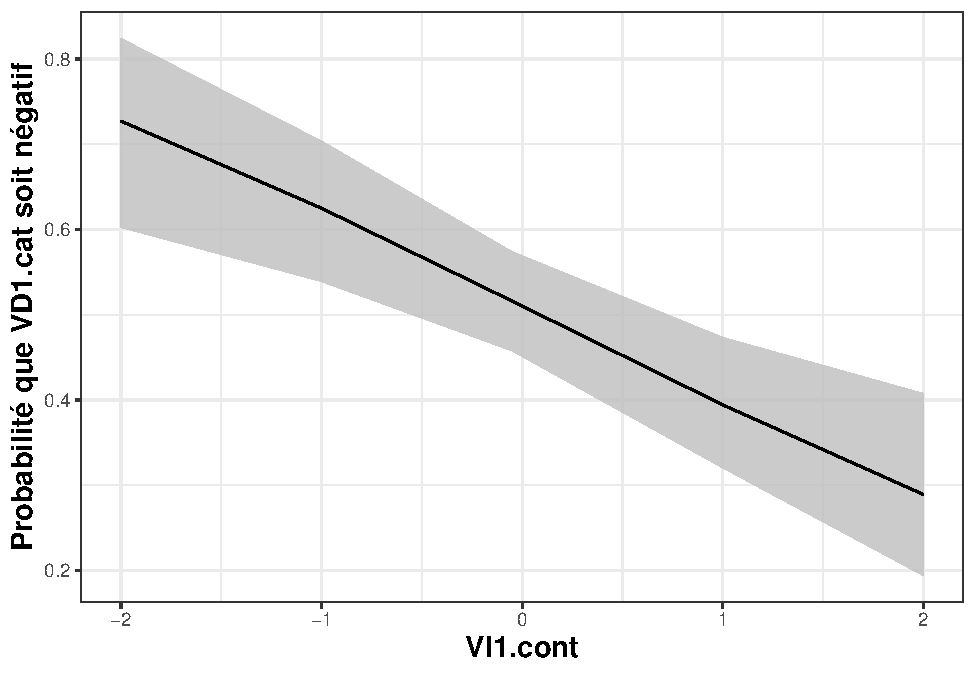
\includegraphics{Manuel_R_independant_files/figure-latex/unnamed-chunk-102-1.pdf}

\hypertarget{interpretation-11}{%
\subsubsection{Interpretation}\label{interpretation-11}}

{[}1{]} ``VI1.cont est lié à VD1.cat lorsque l'on ajuste par l'effet de VI2.cat et VI3.cont: plus VI1.cont est elevé et plus la probabilité que VD1.cat soit négatif est faible (b = -0.47, SE = 0.126, Odds Ratio = 0.625, p = 0.000191)''

\hypertarget{chi-deux-2}{%
\subsection{Chi-deux 2}\label{chi-deux-2}}

\hypertarget{type-de-variables-12}{%
\subsubsection{Type de variables}\label{type-de-variables-12}}

\textbf{Variable Dépendante :} Catégorielle (3 catégories ou +)
\textbf{Variable Indépendante :} Catégorielle (2 catégories ou +)

\hypertarget{packages-nuxe9cessaires-12}{%
\subsubsection{Packages nécessaires}\label{packages-nuxe9cessaires-12}}

\begin{Shaded}
\begin{Highlighting}[]
\KeywordTok{library}\NormalTok{(ggplot2)}
\KeywordTok{library}\NormalTok{(GGally)}
\KeywordTok{library}\NormalTok{(forcats)}
\KeywordTok{library}\NormalTok{(dplyr)}
\KeywordTok{library}\NormalTok{(rcompanion)}
\end{Highlighting}
\end{Shaded}

\hypertarget{donnuxe9es-ruxe9elles-12}{%
\subsubsection{Données réelles}\label{donnuxe9es-ruxe9elles-12}}

\begin{Shaded}
\begin{Highlighting}[]
\CommentTok{# choisissez la ligne appropriée au format de votre fichier de données. }

\CommentTok{# si vos données sont dans un fichier .txt}
\NormalTok{my_data.chideux2 <-}\StringTok{ }\KeywordTok{read.delim}\NormalTok{(}\KeywordTok{file.choose}\NormalTok{())}

\CommentTok{# si vos données sont dans un fichier .csv}
\NormalTok{my_data.chideux2 <-}\StringTok{ }\KeywordTok{read.csv}\NormalTok{(}\KeywordTok{file.choose}\NormalTok{())}

\CommentTok{# si vos données sont dans un fichier .xls / .xlsx}
\NormalTok{my_data.chideux2 <-}\StringTok{ }\KeywordTok{read_excel}\NormalTok{(}\KeywordTok{file.choose}\NormalTok{())}

\CommentTok{# une fois vos données chargées, vous pouvez renommer vos noms de colonnes afin qu'ils correspondent à ceux utilisés dans le code ci-dessous}
\CommentTok{# Si vous ne souhaitez pas renommer vos noms de colonnes, sautez cette étape mais adaptez le code des parties suivantes en lui indiquant les noms de colonnes de vos données.}

\CommentTok{# On crée une nouvelle colonne pour votre variable dépendante catégorielle (remplacez 'votre.nom.de.colonne' par le nom approprié)}
\NormalTok{my_data.chideux2}\OperatorTok{$}\NormalTok{VD1.cat <-}\StringTok{ }\NormalTok{my_data.chideux2}\OperatorTok{$}\StringTok{'votre.nom.de.colonne'}

\CommentTok{# On crée une nouvelle colonne pour votre variable indépendante catégorielle (remplacez 'votre.nom.de.colonne' par le nom approprié)}
\NormalTok{my_data.chideux2}\OperatorTok{$}\NormalTok{VI1.multicat <-}\StringTok{ }\NormalTok{my_data.chideux2}\OperatorTok{$}\StringTok{'votre.nom.de.colonne'}
\end{Highlighting}
\end{Shaded}

\hypertarget{donnuxe9es-fictives-12}{%
\subsubsection{Données fictives}\label{donnuxe9es-fictives-12}}

\begin{Shaded}
\begin{Highlighting}[]
\KeywordTok{set.seed}\NormalTok{(}\DecValTok{4321}\NormalTok{)}
\NormalTok{my_data.chideux2 <-}\StringTok{ }\KeywordTok{data.frame}\NormalTok{(}
  \DataTypeTok{VD1.cat =} \KeywordTok{rbinom}\NormalTok{(}\DecValTok{80}\NormalTok{, }\DecValTok{1}\NormalTok{, }\FloatTok{0.5}\NormalTok{) }\OperatorTok{+}\StringTok{ }\DecValTok{1}\NormalTok{,}
  \DataTypeTok{VI1.multicat =} \KeywordTok{rbinom}\NormalTok{(}\DecValTok{80}\NormalTok{, }\DecValTok{2}\NormalTok{, }\FloatTok{0.5}\NormalTok{) }\OperatorTok{+}\StringTok{ }\DecValTok{1}\NormalTok{)}

\CommentTok{# on renomme les catégories de VD1.cat et VI1.cat pour que les résultats soient plus lisibles}
\NormalTok{my_data.chideux2}\OperatorTok{$}\NormalTok{VD1.cat <-}\StringTok{ }\KeywordTok{fct_recode}\NormalTok{(}\KeywordTok{factor}\NormalTok{(my_data.chideux2}\OperatorTok{$}\NormalTok{VD1.cat), }
                                    \StringTok{"Positif"}\NormalTok{ =}\StringTok{ "1"}\NormalTok{, }
                                    \StringTok{"Negatif"}\NormalTok{ =}\StringTok{ "2"}\NormalTok{) }

\NormalTok{my_data.chideux2}\OperatorTok{$}\NormalTok{VI1.multicat <-}\StringTok{ }\KeywordTok{fct_recode}\NormalTok{(}\KeywordTok{factor}\NormalTok{(my_data.chideux2}\OperatorTok{$}\NormalTok{VI1.multicat), }
                                    \StringTok{"Groupe 1"}\NormalTok{ =}\StringTok{ "1"}\NormalTok{, }
                                    \StringTok{"Groupe 2"}\NormalTok{ =}\StringTok{ "2"}\NormalTok{,}
                                    \StringTok{"Groupe 3"}\NormalTok{ =}\StringTok{ "3"}\NormalTok{) }
\end{Highlighting}
\end{Shaded}

\hypertarget{duxe9claration-du-type-de-variables-11}{%
\subsubsection{Déclaration du type de variables}\label{duxe9claration-du-type-de-variables-11}}

\begin{Shaded}
\begin{Highlighting}[]
\NormalTok{my_data.chideux2}\OperatorTok{$}\NormalTok{VD1.cat <-}\StringTok{ }\KeywordTok{factor}\NormalTok{(my_data.chideux2}\OperatorTok{$}\NormalTok{VD1.cat)}
\NormalTok{my_data.chideux2}\OperatorTok{$}\NormalTok{VI1.multicat <-}\StringTok{ }\KeywordTok{factor}\NormalTok{(my_data.chideux2}\OperatorTok{$}\NormalTok{VI1.multicat)}
\end{Highlighting}
\end{Shaded}

\hypertarget{inspection-des-donnuxe9es-11}{%
\subsubsection{Inspection des données}\label{inspection-des-donnuxe9es-11}}

\begin{Shaded}
\begin{Highlighting}[]
\CommentTok{## Les graphiques situés sur la diagonale représentent la distribution des variables}
\CommentTok{## Les graphiques (ou les valeurs de corrélation) situés au dessus et en dessous de la diagonale représentent l'association entre les différentes variables}
\KeywordTok{ggpairs}\NormalTok{(my_data.chideux2,}
        \DataTypeTok{lower =} \KeywordTok{list}\NormalTok{(}\DataTypeTok{continuous =} \KeywordTok{wrap}\NormalTok{(}\StringTok{"smooth"}\NormalTok{, }\DataTypeTok{alpha =} \FloatTok{0.7}\NormalTok{), }\DataTypeTok{combo =} \StringTok{"box_no_facet"}\NormalTok{),}
        \DataTypeTok{upper =} \KeywordTok{list}\NormalTok{(}\DataTypeTok{combo =} \StringTok{"facetdensity"}\NormalTok{, }\DataTypeTok{discrete =} \StringTok{"facetbar"}\NormalTok{), }
        \DataTypeTok{mapping =} \KeywordTok{aes}\NormalTok{(}\DataTypeTok{alpha =} \FloatTok{0.8}\NormalTok{)) }\OperatorTok{+}\StringTok{ }\KeywordTok{theme_bw}\NormalTok{()}
\end{Highlighting}
\end{Shaded}

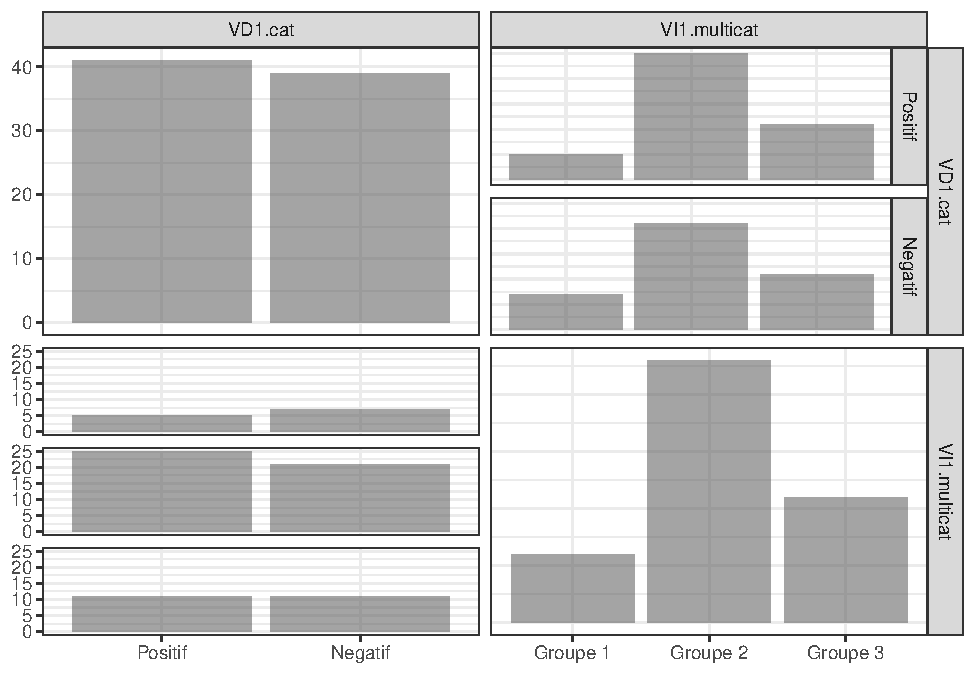
\includegraphics{Manuel_R_independant_files/figure-latex/unnamed-chunk-108-1.pdf}

\hypertarget{analyse-des-donnuxe9es-12}{%
\subsubsection{Analyse des données}\label{analyse-des-donnuxe9es-12}}

\begin{Shaded}
\begin{Highlighting}[]
\CommentTok{# on range les données sous forme de table }
\NormalTok{my_table.chideux2 <-}\StringTok{ }\KeywordTok{with}\NormalTok{(my_data.chideux2, }\KeywordTok{table}\NormalTok{(VI1.multicat, VD1.cat))}

\CommentTok{# calcul du test de chi-deux et stockage des résultats dans l’objet chideux2.test}
\CommentTok{# la correction de Yates peut être obtenue en indiquant l'argument "correct = TRUE"}
\NormalTok{chideux2.test <-}\StringTok{ }\KeywordTok{chisq.test}\NormalTok{(my_table.chideux2, }\DataTypeTok{correct =} \OtherTok{FALSE}\NormalTok{)}

\CommentTok{# calcul des proportions de VD1.cat dans chaque modalité de VI1.cat}
\NormalTok{description.chideux2 <-}\StringTok{ }\KeywordTok{data.frame}\NormalTok{(my_table.chideux2) }\OperatorTok
\StringTok{    }\KeywordTok{group_by}\NormalTok{(VI1.multicat) }\OperatorTok
\StringTok{    }\KeywordTok{summarise}\NormalTok{(}\DataTypeTok{proportion =}\NormalTok{ Freq }\OperatorTok{/}\StringTok{ }\KeywordTok{sum}\NormalTok{(Freq),}
              \DataTypeTok{VD1.cat =}\NormalTok{ VD1.cat)}
\CommentTok{# tests post hoc comparant toutes les modalités de VI1.multicat entre elles (sans correction de yates mais en corrigeant la p-value ajustée avec une méthode de bonferroni)}
\NormalTok{posthoc.chideux2 <-}\StringTok{ }\KeywordTok{pairwiseNominalIndependence}\NormalTok{(my_table.chideux2,}
                            \DataTypeTok{fisher =} \OtherTok{FALSE}\NormalTok{,}
                            \DataTypeTok{gtest =} \OtherTok{FALSE}\NormalTok{,}
                            \DataTypeTok{correct =} \StringTok{"none"}\NormalTok{,}
                            \DataTypeTok{method =} \StringTok{"bonferroni"}\NormalTok{)}

\CommentTok{# calcul de la taille d'effet de VI1.multicat sur VD1.cat (odds ratio comparant le groupe 1 au groupe 2, le groupe 1 au groupe 3 et le groupe 2 au groupe 3)}
\NormalTok{odds.ratio.chideux2.grp1.grp2 <-}\StringTok{ }\NormalTok{(my_table.chideux2[}\DecValTok{1}\NormalTok{,}\DecValTok{1}\NormalTok{]}\OperatorTok{/}\NormalTok{my_table.chideux2[}\DecValTok{1}\NormalTok{,}\DecValTok{2}\NormalTok{])}\OperatorTok{/}\NormalTok{(my_table.chideux2[}\DecValTok{2}\NormalTok{,}\DecValTok{1}\NormalTok{]}\OperatorTok{/}\NormalTok{my_table.chideux2[}\DecValTok{2}\NormalTok{,}\DecValTok{2}\NormalTok{])}
\NormalTok{odds.ratio.chideux2.grp1.grp3 <-}\StringTok{ }\NormalTok{(my_table.chideux2[}\DecValTok{1}\NormalTok{,}\DecValTok{1}\NormalTok{]}\OperatorTok{/}\NormalTok{my_table.chideux2[}\DecValTok{1}\NormalTok{,}\DecValTok{2}\NormalTok{])}\OperatorTok{/}\NormalTok{(my_table.chideux2[}\DecValTok{3}\NormalTok{,}\DecValTok{1}\NormalTok{]}\OperatorTok{/}\NormalTok{my_table.chideux2[}\DecValTok{3}\NormalTok{,}\DecValTok{2}\NormalTok{])}
\NormalTok{odds.ratio.chideux2.grp2.grp3 <-}\StringTok{ }\NormalTok{(my_table.chideux2[}\DecValTok{2}\NormalTok{,}\DecValTok{1}\NormalTok{]}\OperatorTok{/}\NormalTok{my_table.chideux2[}\DecValTok{2}\NormalTok{,}\DecValTok{2}\NormalTok{])}\OperatorTok{/}\NormalTok{(my_table.chideux2[}\DecValTok{3}\NormalTok{,}\DecValTok{1}\NormalTok{]}\OperatorTok{/}\NormalTok{my_table.chideux2[}\DecValTok{3}\NormalTok{,}\DecValTok{2}\NormalTok{])}

\CommentTok{# obtention des résultats tableau de contigence et des proportions  }
\NormalTok{my_table.chideux2; description.chideux2}
\end{Highlighting}
\end{Shaded}

\begin{verbatim}
##             VD1.cat
## VI1.multicat Positif Negatif
##     Groupe 1       5       7
##     Groupe 2      25      21
##     Groupe 3      11      11
\end{verbatim}

\begin{verbatim}
## # A tibble: 6 x 3
## # Groups:   VI1.multicat [3]
##   VI1.multicat proportion VD1.cat
##   <fct>             <dbl> <fct>  
## 1 Groupe 1          0.417 Positif
## 2 Groupe 1          0.583 Negatif
## 3 Groupe 2          0.543 Positif
## 4 Groupe 2          0.457 Negatif
## 5 Groupe 3          0.5   Positif
## 6 Groupe 3          0.5   Negatif
\end{verbatim}

\begin{Shaded}
\begin{Highlighting}[]
\CommentTok{# obtention du test de chi deux }
\NormalTok{chideux2.test}
\end{Highlighting}
\end{Shaded}

\begin{verbatim}
## 
## 	Pearson's Chi-squared test
## 
## data:  my_table.chideux2
## X-squared = 0.63155, df = 2, p-value = 0.7292
\end{verbatim}

\begin{Shaded}
\begin{Highlighting}[]
\CommentTok{# obtention des tests post hoc }
\NormalTok{posthoc.chideux2}
\end{Highlighting}
\end{Shaded}

\begin{verbatim}
##            Comparison p.Chisq p.adj.Chisq
## 1 Groupe 1 : Groupe 2   0.647           1
## 2 Groupe 1 : Groupe 3   0.916           1
## 3 Groupe 2 : Groupe 3   0.939           1
\end{verbatim}

\begin{Shaded}
\begin{Highlighting}[]
\CommentTok{# obtention des tailles d'effet}
\NormalTok{odds.ratio.chideux2.grp1.grp2; odds.ratio.chideux2.grp1.grp3; odds.ratio.chideux2.grp2.grp3}
\end{Highlighting}
\end{Shaded}

\begin{verbatim}
## [1] 0.6
\end{verbatim}

\begin{verbatim}
## [1] 0.7142857
\end{verbatim}

\begin{verbatim}
## [1] 1.190476
\end{verbatim}

\hypertarget{graphique-12}{%
\subsubsection{Graphique}\label{graphique-12}}

\begin{Shaded}
\begin{Highlighting}[]
\KeywordTok{ggplot}\NormalTok{(my_data.chideux2, }\KeywordTok{aes}\NormalTok{(}\DataTypeTok{x =} \KeywordTok{factor}\NormalTok{(VI1.multicat), }\DataTypeTok{fill =}\NormalTok{ VD1.cat)) }\OperatorTok{+}\StringTok{ }
\StringTok{  }\KeywordTok{geom_bar}\NormalTok{(}\DataTypeTok{stat =} \StringTok{"count"}\NormalTok{, }\DataTypeTok{position =} \KeywordTok{position_dodge2}\NormalTok{())  }\OperatorTok{+}
\StringTok{  }\KeywordTok{scale_fill_grey}\NormalTok{(}\DataTypeTok{start =} \FloatTok{0.8}\NormalTok{, }\DataTypeTok{end =} \FloatTok{0.5}\NormalTok{) }\OperatorTok{+}
\StringTok{  }\KeywordTok{ylab}\NormalTok{(}\StringTok{"Nombre de personnes"}\NormalTok{) }\OperatorTok{+}\StringTok{ }\KeywordTok{xlab}\NormalTok{(}\StringTok{"VI1.cat"}\NormalTok{) }\OperatorTok{+}\StringTok{ }
\StringTok{  }\KeywordTok{theme_bw}\NormalTok{() }\OperatorTok{+}\StringTok{ }
\StringTok{  }\KeywordTok{theme}\NormalTok{(}\DataTypeTok{axis.title.y =} \KeywordTok{element_text}\NormalTok{(}\DataTypeTok{size =} \DecValTok{14}\NormalTok{, }\DataTypeTok{hjust =} \FloatTok{0.5}\NormalTok{, }\DataTypeTok{face =} \StringTok{"bold"}\NormalTok{), }
        \DataTypeTok{axis.title.x =} \KeywordTok{element_text}\NormalTok{(}\DataTypeTok{face =} \StringTok{"bold"}\NormalTok{, }\DataTypeTok{size =} \DecValTok{14}\NormalTok{, }\DataTypeTok{hjust =} \FloatTok{0.5}\NormalTok{))}
\end{Highlighting}
\end{Shaded}

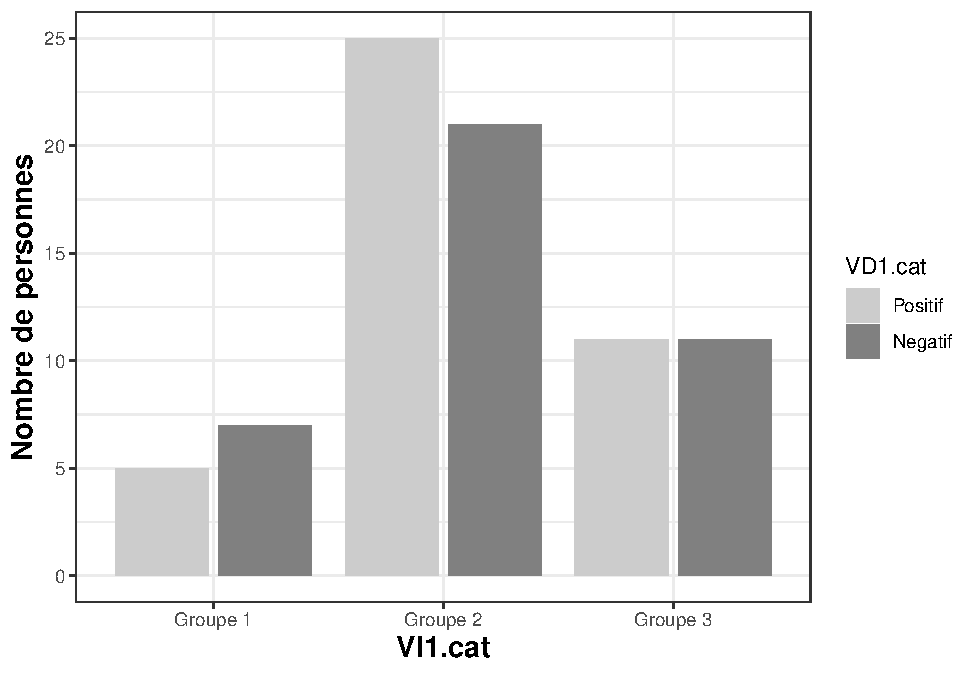
\includegraphics{Manuel_R_independant_files/figure-latex/unnamed-chunk-110-1.pdf}

\hypertarget{interpretation-12}{%
\subsubsection{Interpretation}\label{interpretation-12}}

{[}1{]} ``La proportion de cas ayant une modalité de VD1.cat égale à 1 (positif) ne diffère pas statistiquement entre les groupes 1, 2 et 3 (X² = 0.632, p = 0.729). Plus précisément, ni la différence entre les groupes 1 et 2 (odds ratio = 0.6, p non ajusté = 0.647), ni la différence entre les groupes 1 et 3 (odds ratio = 0.714, p non ajusté = 0.916), ni la différence entre les groupes 2 et 3 (odds ratio = 1.19, p non ajusté = 0.939), n'atteint la significativité.''

\hypertarget{ruxe9gression-logistique-multinomiale-1}{%
\subsection{Régression logistique multinomiale 1}\label{ruxe9gression-logistique-multinomiale-1}}

\hypertarget{type-de-variables-13}{%
\subsubsection{Type de variables}\label{type-de-variables-13}}

\textbf{Variable Dépendante :} Catégorielle (3 catégories ou +)
\textbf{Variable Indépendante :} Numérique

\hypertarget{packages-nuxe9cessaires-13}{%
\subsubsection{Packages nécessaires}\label{packages-nuxe9cessaires-13}}

\begin{Shaded}
\begin{Highlighting}[]
\KeywordTok{library}\NormalTok{(ggplot2)}
\KeywordTok{library}\NormalTok{(GGally)}
\KeywordTok{library}\NormalTok{(forcats)}
\KeywordTok{library}\NormalTok{(car)}
\KeywordTok{library}\NormalTok{(emmeans)}
\KeywordTok{library}\NormalTok{(nnet)}
\KeywordTok{library}\NormalTok{(tidyr)}
\end{Highlighting}
\end{Shaded}

\hypertarget{donnuxe9es-ruxe9elles-13}{%
\subsubsection{Données réelles}\label{donnuxe9es-ruxe9elles-13}}

\begin{Shaded}
\begin{Highlighting}[]
\CommentTok{# choisissez la ligne appropriée au format de votre fichier de données. }

\CommentTok{# si vos données sont dans un fichier .txt}
\NormalTok{my_data.regmultinom1 <-}\StringTok{ }\KeywordTok{read.delim}\NormalTok{(}\KeywordTok{file.choose}\NormalTok{())}

\CommentTok{# si vos données sont dans un fichier .csv}
\NormalTok{my_data.regmultinom1 <-}\StringTok{ }\KeywordTok{read.csv}\NormalTok{(}\KeywordTok{file.choose}\NormalTok{())}

\CommentTok{# si vos données sont dans un fichier .xls / .xlsx}
\NormalTok{my_data.regmultinom1 <-}\StringTok{ }\KeywordTok{read_excel}\NormalTok{(}\KeywordTok{file.choose}\NormalTok{())}

\CommentTok{# une fois vos données chargées, vous pouvez renommer vos noms de colonnes afin qu'ils correspondent à ceux utilisés dans le code ci-dessous}
\CommentTok{# Si vous ne souhaitez pas renommer vos noms de colonnes, sautez cette étape mais adaptez le code des parties suivantes en lui indiquant les noms de colonnes de vos données.}

\CommentTok{# On crée une nouvelle colonne pour votre variable dépendante multicatégorielle (remplacez 'votre.nom.de.colonne' par le nom approprié)}
\NormalTok{my_data.regmultinom1}\OperatorTok{$}\NormalTok{VD1.multicat <-}\StringTok{ }\NormalTok{my_data.regmultinom1}\OperatorTok{$}\StringTok{'votre.nom.de.colonne'}

\CommentTok{# On crée une nouvelle colonne pour votre variable indépendante continue (remplacez 'votre.nom.de.colonne' par le nom approprié)}
\NormalTok{my_data.regmultinom1}\OperatorTok{$}\NormalTok{VI1.cont <-}\StringTok{ }\NormalTok{my_data.regmultinom1}\OperatorTok{$}\StringTok{'votre.nom.de.colonne'}
\end{Highlighting}
\end{Shaded}

\hypertarget{donnuxe9es-fictives-13}{%
\subsubsection{Données fictives}\label{donnuxe9es-fictives-13}}

\begin{Shaded}
\begin{Highlighting}[]
\KeywordTok{set.seed}\NormalTok{(}\DecValTok{4321}\NormalTok{)}
\NormalTok{my_data.regmultinom1 <-}\StringTok{ }\KeywordTok{data.frame}\NormalTok{(}
  \DataTypeTok{VD1.multicat =} \KeywordTok{rep}\NormalTok{(}\KeywordTok{c}\NormalTok{(}\DecValTok{1}\NormalTok{, }\DecValTok{2}\NormalTok{, }\DecValTok{3}\NormalTok{), }\DataTypeTok{each=}\DecValTok{100}\NormalTok{),}
  \DataTypeTok{VI1.cont =} \KeywordTok{c}\NormalTok{(}\KeywordTok{rnorm}\NormalTok{(}\DecValTok{100}\NormalTok{) }\OperatorTok{-}\StringTok{ }\FloatTok{0.25}\NormalTok{, }\KeywordTok{rnorm}\NormalTok{(}\DecValTok{100}\NormalTok{), }\KeywordTok{rnorm}\NormalTok{(}\DecValTok{100}\NormalTok{) }\OperatorTok{+}\StringTok{ }\FloatTok{0.25}\NormalTok{))}

\CommentTok{# on renomme les catégories de VD1.cat pour que les résultats soient plus lisibles}
\NormalTok{my_data.regmultinom1}\OperatorTok{$}\NormalTok{VD1.multicat <-}\StringTok{ }\KeywordTok{fct_recode}\NormalTok{(}\KeywordTok{factor}\NormalTok{(my_data.regmultinom1}\OperatorTok{$}\NormalTok{VD1.multicat), }
                                            \StringTok{"Categorie 1"}\NormalTok{ =}\StringTok{ "1"}\NormalTok{, }
                                            \StringTok{"Categorie 2"}\NormalTok{ =}\StringTok{ "2"}\NormalTok{,}
                                            \StringTok{"Categorie 3"}\NormalTok{ =}\StringTok{ "3"}\NormalTok{) }
\end{Highlighting}
\end{Shaded}

\hypertarget{duxe9claration-du-type-de-variables-12}{%
\subsubsection{Déclaration du type de variables}\label{duxe9claration-du-type-de-variables-12}}

\begin{Shaded}
\begin{Highlighting}[]
\NormalTok{my_data.regmultinom1}\OperatorTok{$}\NormalTok{VD1.multicat <-}\StringTok{ }\KeywordTok{factor}\NormalTok{(my_data.regmultinom1}\OperatorTok{$}\NormalTok{VD1.multicat)}
\NormalTok{my_data.regmultinom1}\OperatorTok{$}\NormalTok{VI1.cont <-}\StringTok{ }\KeywordTok{as.numeric}\NormalTok{(}\KeywordTok{as.character}\NormalTok{(my_data.regmultinom1}\OperatorTok{$}\NormalTok{VI1.cont))}
\end{Highlighting}
\end{Shaded}

\hypertarget{inspection-des-donnuxe9es-12}{%
\subsubsection{Inspection des données}\label{inspection-des-donnuxe9es-12}}

\begin{Shaded}
\begin{Highlighting}[]
\CommentTok{## Les graphiques situés sur la diagonale représentent la distribution des variables}
\CommentTok{## Les graphiques (ou les valeurs de corrélation) situés au dessus et en dessous de la diagonale représentent l'association entre les différentes variables}
\KeywordTok{ggpairs}\NormalTok{(my_data.regmultinom1,}
        \DataTypeTok{lower =} \KeywordTok{list}\NormalTok{(}\DataTypeTok{continuous =} \KeywordTok{wrap}\NormalTok{(}\StringTok{"smooth"}\NormalTok{, }\DataTypeTok{alpha =} \FloatTok{0.7}\NormalTok{), }\DataTypeTok{combo =} \StringTok{"box_no_facet"}\NormalTok{),}
        \DataTypeTok{upper =} \KeywordTok{list}\NormalTok{(}\DataTypeTok{combo =} \StringTok{"facetdensity"}\NormalTok{, }\DataTypeTok{discrete =} \StringTok{"facetbar"}\NormalTok{), }
        \DataTypeTok{mapping =} \KeywordTok{aes}\NormalTok{(}\DataTypeTok{alpha =} \FloatTok{0.8}\NormalTok{)) }\OperatorTok{+}\StringTok{ }\KeywordTok{theme_bw}\NormalTok{()}
\end{Highlighting}
\end{Shaded}

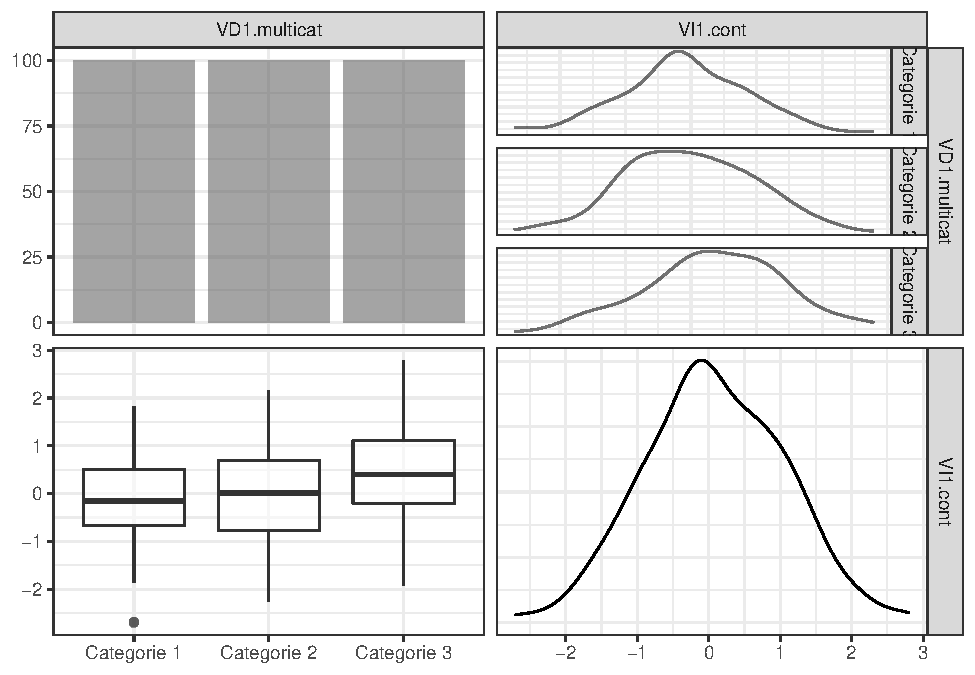
\includegraphics{Manuel_R_independant_files/figure-latex/unnamed-chunk-116-1.pdf}

\hypertarget{analyse-des-donnuxe9es-13}{%
\subsubsection{Analyse des données}\label{analyse-des-donnuxe9es-13}}

\begin{Shaded}
\begin{Highlighting}[]
\CommentTok{# calcul de la régression logistique multinomiale et stockage des résultats dans l’objet regmultinom1.test}
\NormalTok{regmultinom1.test <-}\StringTok{ }\KeywordTok{multinom}\NormalTok{(}\DataTypeTok{formula =}\NormalTok{ VD1.multicat }\OperatorTok{~}\StringTok{ }\NormalTok{VI1.cont, }
                              \DataTypeTok{data =}\NormalTok{ my_data.regmultinom1)}
\end{Highlighting}
\end{Shaded}

\begin{verbatim}
## # weights:  9 (4 variable)
## initial  value 329.583687 
## final  value 321.470377 
## converged
\end{verbatim}

\begin{Shaded}
\begin{Highlighting}[]
\NormalTok{X2.regmultinom1 <-}\StringTok{ }\KeywordTok{as.numeric}\NormalTok{(}\KeywordTok{as.character}\NormalTok{(}\KeywordTok{Anova}\NormalTok{(regmultinom1.test)}\OperatorTok{$}\StringTok{'LR Chisq'}\NormalTok{))}
\end{Highlighting}
\end{Shaded}

\begin{verbatim}
## # weights:  6 (2 variable)
## initial  value 329.583687 
## final  value 329.583687 
## converged
\end{verbatim}

\begin{Shaded}
\begin{Highlighting}[]
\NormalTok{p.regmultinom1 <-}\StringTok{ }\KeywordTok{as.numeric}\NormalTok{(}\KeywordTok{as.character}\NormalTok{(}\KeywordTok{Anova}\NormalTok{(regmultinom1.test)}\OperatorTok{$}\StringTok{'Pr(>Chisq)'}\NormalTok{))}
\end{Highlighting}
\end{Shaded}

\begin{verbatim}
## # weights:  6 (2 variable)
## initial  value 329.583687 
## final  value 329.583687 
## converged
\end{verbatim}

\begin{Shaded}
\begin{Highlighting}[]
\CommentTok{# tests post hoc explorant l'effet de VD1.cont sur chaque modalité de VD1.multicat}
\NormalTok{posthoc.regmultinom1 <-}\StringTok{ }\KeywordTok{emtrends}\NormalTok{(regmultinom1.test, }
                                 \DataTypeTok{var =} \StringTok{"VI1.cont"}\NormalTok{, }\OperatorTok{~}\StringTok{ }\NormalTok{VD1.multicat)}


\CommentTok{# tailles d'effet de VI1.cont sur VD1.multicat (odds ratio comparant l'effet de VI1.cont sur VD1.multicat entre les groupes 1 et 2 puis entre les groupes 1 et 3)}
\NormalTok{odds.ratio.regmultinom1 <-}\StringTok{ }\KeywordTok{exp}\NormalTok{(}\KeywordTok{coef}\NormalTok{(}\KeywordTok{summary}\NormalTok{(regmultinom1.test)))}

\CommentTok{# Obtention des résultats de la régression logistique multinomiale évaluant l'effet global de VI1.cont sur VD1.cat }
\KeywordTok{data.frame}\NormalTok{(}\KeywordTok{cbind}\NormalTok{(}
  \DataTypeTok{Variable =} \StringTok{"VI1.cont"}\NormalTok{, }
  \StringTok{"X2"}\NormalTok{ =}\StringTok{ }\NormalTok{X2.regmultinom1,}
  \StringTok{"p"}\NormalTok{ =}\StringTok{ }\NormalTok{p.regmultinom1))}
\end{Highlighting}
\end{Shaded}

\begin{verbatim}
##   Variable              X2                    p
## 1 VI1.cont 16.226618550692 0.000299526017216273
\end{verbatim}

\begin{Shaded}
\begin{Highlighting}[]
\CommentTok{# obtention des tests post hoc :}

\CommentTok{## explorant l'effet de VD1.cont sur chaque modalité de VD1.multicat}
\KeywordTok{test}\NormalTok{(posthoc.regmultinom1, }\DataTypeTok{adjust =} \StringTok{"mvt"}\NormalTok{)}
\end{Highlighting}
\end{Shaded}

\begin{verbatim}
##  VD1.multicat VI1.cont.trend     SE df t.ratio p.value
##  Categorie 1         -0.0752 0.0287  4 -2.616  0.1212 
##  Categorie 2         -0.0372 0.0285  4 -1.302  0.4654 
##  Categorie 3          0.1123 0.0291  4  3.855  0.0389 
## 
## P value adjustment: mvt method for 3 tests
\end{verbatim}

\begin{Shaded}
\begin{Highlighting}[]
\CommentTok{##comparant l'effet de VI1.cont entre chaque modalité de VD1.multicat}
\KeywordTok{pairs}\NormalTok{(posthoc.regmultinom1)}
\end{Highlighting}
\end{Shaded}

\begin{verbatim}
##  contrast                  estimate     SE df t.ratio p.value
##  Categorie 1 - Categorie 2   -0.038 0.0493  4 -0.771  0.7385 
##  Categorie 1 - Categorie 3   -0.187 0.0503  4 -3.724  0.0436 
##  Categorie 2 - Categorie 3   -0.149 0.0500  4 -2.990  0.0843 
## 
## P value adjustment: tukey method for comparing a family of 3 estimates
\end{verbatim}

\begin{Shaded}
\begin{Highlighting}[]
\CommentTok{# des tailles d'effet}
\NormalTok{odds.ratio.regmultinom1}
\end{Highlighting}
\end{Shaded}

\begin{verbatim}
##             (Intercept) VI1.cont
## Categorie 2   1.0083688 1.122676
## Categorie 3   0.9252016 1.768750
\end{verbatim}

\hypertarget{graphique-13}{%
\subsubsection{Graphique}\label{graphique-13}}

\begin{Shaded}
\begin{Highlighting}[]
\NormalTok{crude.slope.regmultinom1 <-}\StringTok{ }\KeywordTok{as.data.frame}\NormalTok{(}
  \KeywordTok{effect}\NormalTok{(}
    \DataTypeTok{term =} \StringTok{"VI1.cont"}\NormalTok{, }
    \DataTypeTok{mod =}\NormalTok{ regmultinom1.test))}

\NormalTok{crude.slope.regmultinom1.long <-crude.slope.regmultinom1 }\OperatorTok\StringTok{ }
\StringTok{    }\NormalTok{dplyr}\OperatorTok{::}\KeywordTok{select}\NormalTok{(VI1.cont, }
\NormalTok{                  prob.Categorie}\FloatTok{.1}\NormalTok{, }
\NormalTok{                  prob.Categorie}\FloatTok{.2}\NormalTok{,}
\NormalTok{                  prob.Categorie}\FloatTok{.3}\NormalTok{) }\OperatorTok
\StringTok{    }\KeywordTok{pivot_longer}\NormalTok{(}\OperatorTok{-}\NormalTok{VI1.cont, }
        \DataTypeTok{names_to=}\StringTok{"var"}\NormalTok{,}
        \DataTypeTok{values_to=}\StringTok{"VD"}\NormalTok{)}

\NormalTok{crude.slope.regmultinom1.long}\OperatorTok{$}\NormalTok{var<-}\StringTok{ }\KeywordTok{fct_recode}\NormalTok{(crude.slope.regmultinom1.long}\OperatorTok{$}\NormalTok{var, }
           \StringTok{"Categorie 1"}\NormalTok{ =}\StringTok{ "prob.Categorie.1"}\NormalTok{, }
           \StringTok{"Categorie 2"}\NormalTok{ =}\StringTok{ "prob.Categorie.2"}\NormalTok{,}
           \StringTok{"Categorie 3"}\NormalTok{ =}\StringTok{ "prob.Categorie.3"}\NormalTok{)}


\KeywordTok{ggplot}\NormalTok{(crude.slope.regmultinom1.long) }\OperatorTok{+}\StringTok{ }
\StringTok{  }\KeywordTok{geom_line}\NormalTok{(}\KeywordTok{aes}\NormalTok{(}\DataTypeTok{x =}\NormalTok{ VI1.cont, }\DataTypeTok{y =}\NormalTok{ VD, }\DataTypeTok{color =}\NormalTok{ var),  }\DataTypeTok{size =} \DecValTok{1}\NormalTok{) }\OperatorTok{+}\StringTok{ }
\StringTok{  }\KeywordTok{facet_wrap}\NormalTok{(}\OperatorTok{~}\NormalTok{var) }\OperatorTok{+}
\StringTok{  }\KeywordTok{ylab}\NormalTok{(}\StringTok{"Probabilité"}\NormalTok{) }\OperatorTok{+}\StringTok{ }
\StringTok{  }\KeywordTok{xlab}\NormalTok{(}\StringTok{"VI1.cont"}\NormalTok{) }\OperatorTok{+}
\StringTok{  }\KeywordTok{theme_bw}\NormalTok{() }\OperatorTok{+}\StringTok{ }
\StringTok{  }\KeywordTok{theme}\NormalTok{(}\DataTypeTok{axis.title.y =} \KeywordTok{element_text}\NormalTok{(}\DataTypeTok{size =} \DecValTok{14}\NormalTok{, }\DataTypeTok{hjust =} \FloatTok{0.5}\NormalTok{, }\DataTypeTok{face=}\StringTok{"bold"}\NormalTok{), }
        \DataTypeTok{axis.title.x =} \KeywordTok{element_text}\NormalTok{(}\DataTypeTok{face=}\StringTok{"bold"}\NormalTok{, }\DataTypeTok{size =} \DecValTok{14}\NormalTok{, }\DataTypeTok{hjust =} \FloatTok{0.5}\NormalTok{)) }\OperatorTok{+}
\StringTok{  }\KeywordTok{guides}\NormalTok{(}\DataTypeTok{color=}\OtherTok{FALSE}\NormalTok{) }
\end{Highlighting}
\end{Shaded}

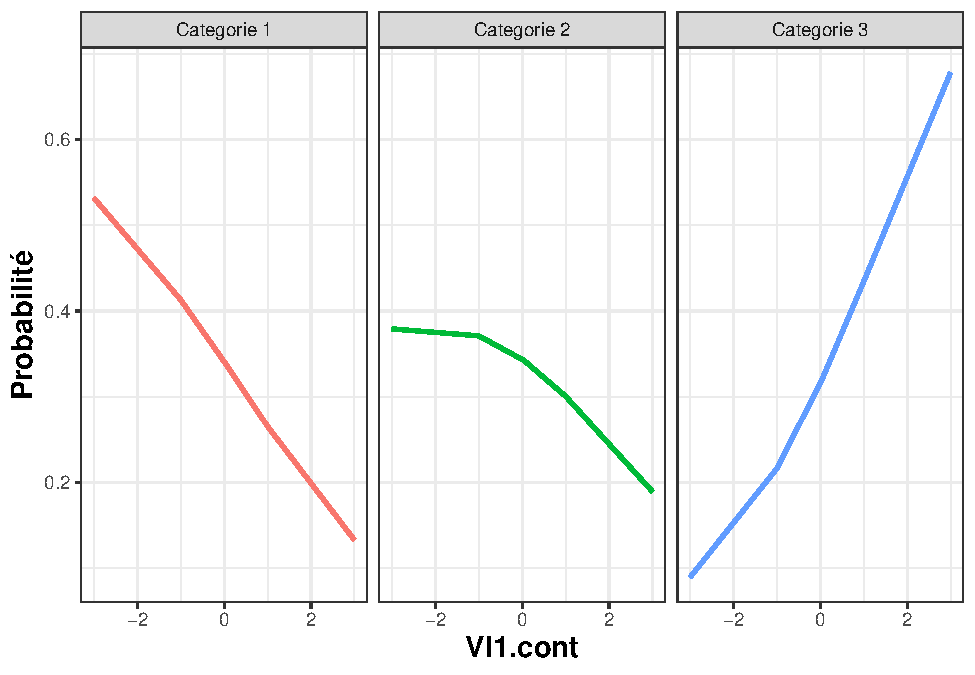
\includegraphics{Manuel_R_independant_files/figure-latex/unnamed-chunk-118-1.pdf}

\hypertarget{interpretation-13}{%
\subsubsection{Interpretation}\label{interpretation-13}}

{[}1{]} ``Les valeurs de VI1.cont sont liées à celles de VD1.multicat (X² = 16.227, p = 3e-04). Plus précisement, plus VI1.cont est élevée et plus la probabilité de Catégorie 3 augmente (valeur p ajustée = 0.039). En revanche, aucun lien statistiquement significatif entre VI1.cont et les catégories 1 et 2 de VD1.multicat (toutes valeurs p ajustées \textgreater{} 0.121). Ces différences entre les catégories 1 et 2 vs.~catégorie 3 sont significatives ou marginalement significatives (toutes valeurs p ajustées \textless{} 0.084)''

\hypertarget{ruxe9gression-logistique-multinomiale-2}{%
\subsection{Régression logistique multinomiale 2}\label{ruxe9gression-logistique-multinomiale-2}}

\hypertarget{type-de-variables-14}{%
\subsubsection{Type de variables}\label{type-de-variables-14}}

\textbf{Variable Dépendante :} Catégorielle (3 catégories ou +)
\textbf{Variables Indépendantes :} Catégorielles (2 catégories ou +)

\hypertarget{packages-nuxe9cessaires-14}{%
\subsubsection{Packages nécessaires}\label{packages-nuxe9cessaires-14}}

\begin{Shaded}
\begin{Highlighting}[]
\KeywordTok{library}\NormalTok{(ggplot2)}
\KeywordTok{library}\NormalTok{(GGally)}
\KeywordTok{library}\NormalTok{(forcats)}
\KeywordTok{library}\NormalTok{(dplyr)}
\KeywordTok{library}\NormalTok{(emmeans)}
\KeywordTok{library}\NormalTok{(broom)}
\KeywordTok{library}\NormalTok{(nnet)}
\KeywordTok{library}\NormalTok{(car)}
\end{Highlighting}
\end{Shaded}

\hypertarget{donnuxe9es-ruxe9elles-14}{%
\subsubsection{Données réelles}\label{donnuxe9es-ruxe9elles-14}}

\begin{Shaded}
\begin{Highlighting}[]
\CommentTok{# choisissez la ligne appropriée au format de votre fichier de données. }

\CommentTok{# si vos données sont dans un fichier .txt}
\NormalTok{my_data.regmultinom2 <-}\StringTok{ }\KeywordTok{read.delim}\NormalTok{(}\KeywordTok{file.choose}\NormalTok{())}

\CommentTok{# si vos données sont dans un fichier .csv}
\NormalTok{my_data.regmultinom2 <-}\StringTok{ }\KeywordTok{read.csv}\NormalTok{(}\KeywordTok{file.choose}\NormalTok{())}

\CommentTok{# si vos données sont dans un fichier .xls / .xlsx}
\NormalTok{my_data.regmultinom2 <-}\StringTok{ }\KeywordTok{read_excel}\NormalTok{(}\KeywordTok{file.choose}\NormalTok{())}

\CommentTok{# une fois vos données chargées, vous pouvez renommer vos noms de colonnes afin qu'ils correspondent à ceux utilisés dans le code ci-dessous}
\CommentTok{# Si vous ne souhaitez pas renommer vos noms de colonnes, sautez cette étape mais adaptez le code des parties suivantes en lui indiquant les noms de colonnes de vos données.}

\CommentTok{# On crée une nouvelle colonne pour votre variable dépendante multicatégorielle (remplacez 'votre.nom.de.colonne' par le nom approprié)}
\NormalTok{my_data.regmultinom2}\OperatorTok{$}\NormalTok{VD1.multicat <-}\StringTok{ }\NormalTok{my_data.regmultinom2}\OperatorTok{$}\StringTok{'votre.nom.de.colonne'}

\CommentTok{# On crée une nouvelle colonne pour vos variables indépendantes catégorielles (remplacez 'votre.nom.de.colonne' par les noms appropriés)}
\NormalTok{my_data.regmultinom2}\OperatorTok{$}\NormalTok{VI1.multicat <-}\StringTok{ }\NormalTok{my_data.regmultinom2}\OperatorTok{$}\StringTok{'votre.nom.de.colonne'}
\NormalTok{my_data.regmultinom2}\OperatorTok{$}\NormalTok{VI2.cat <-}\StringTok{ }\NormalTok{my_data.regmultinom2}\OperatorTok{$}\StringTok{'votre.nom.de.colonne'}
\end{Highlighting}
\end{Shaded}

\hypertarget{donnuxe9es-fictives-14}{%
\subsubsection{Données fictives}\label{donnuxe9es-fictives-14}}

\begin{Shaded}
\begin{Highlighting}[]
\KeywordTok{set.seed}\NormalTok{(}\DecValTok{4321}\NormalTok{)}
\NormalTok{multinom2 <-}\StringTok{ }\KeywordTok{rbinom}\NormalTok{(}\DecValTok{300}\NormalTok{, }\DecValTok{1}\NormalTok{, }\FloatTok{0.8}\NormalTok{)}
\NormalTok{my_data.multinom2 <-}\StringTok{ }\KeywordTok{data.frame}\NormalTok{(}
  \DataTypeTok{VD1.multicat =}\NormalTok{ (}\KeywordTok{rbinom}\NormalTok{(}\DecValTok{300}\NormalTok{, }\DecValTok{2}\NormalTok{, }\FloatTok{0.5}\NormalTok{)}\OperatorTok{*}\NormalTok{multinom2 }\OperatorTok{+}\StringTok{ }\DecValTok{1}\NormalTok{),}
  \DataTypeTok{VI1.multicat =}\NormalTok{ (}\KeywordTok{rbinom}\NormalTok{(}\DecValTok{300}\NormalTok{, }\DecValTok{2}\NormalTok{, }\FloatTok{0.5}\NormalTok{)}\OperatorTok{*}\NormalTok{multinom2 }\OperatorTok{+}\StringTok{ }\DecValTok{1}\NormalTok{),}
  \DataTypeTok{VI2.cat =}\NormalTok{ (}\KeywordTok{rbinom}\NormalTok{(}\DecValTok{300}\NormalTok{, }\DecValTok{1}\NormalTok{, }\FloatTok{0.6}\NormalTok{) }\OperatorTok{+}\StringTok{ }\DecValTok{1}\NormalTok{))}


\CommentTok{# on renomme les catégories de VD1.multicat, VI1.multicat et VI2.cat pour que les résultats soient plus lisibles}
\NormalTok{my_data.multinom2}\OperatorTok{$}\NormalTok{VD1.multicat <-}\StringTok{ }\KeywordTok{fct_recode}\NormalTok{(}\KeywordTok{factor}\NormalTok{(my_data.multinom2}\OperatorTok{$}\NormalTok{VD1.multicat), }
                                    \StringTok{"Categorie 1"}\NormalTok{ =}\StringTok{ "1"}\NormalTok{, }
                                    \StringTok{"Categorie 2"}\NormalTok{ =}\StringTok{ "2"}\NormalTok{,}
                                    \StringTok{"Categorie 3"}\NormalTok{ =}\StringTok{ "3"}\NormalTok{) }

\NormalTok{my_data.multinom2}\OperatorTok{$}\NormalTok{VI1.multicat <-}\StringTok{ }\KeywordTok{fct_recode}\NormalTok{(}\KeywordTok{factor}\NormalTok{(my_data.multinom2}\OperatorTok{$}\NormalTok{VI1.multicat), }
                                    \StringTok{"Groupe 1"}\NormalTok{ =}\StringTok{ "1"}\NormalTok{, }
                                    \StringTok{"Groupe 2"}\NormalTok{ =}\StringTok{ "2"}\NormalTok{,}
                                    \StringTok{"Groupe 3"}\NormalTok{ =}\StringTok{ "3"}\NormalTok{) }

\NormalTok{my_data.multinom2}\OperatorTok{$}\NormalTok{VI2.cat <-}\StringTok{ }\KeywordTok{fct_recode}\NormalTok{(}\KeywordTok{factor}\NormalTok{(my_data.multinom2}\OperatorTok{$}\NormalTok{VI2.cat), }
                                    \StringTok{"Caracteristique 1"}\NormalTok{ =}\StringTok{ "1"}\NormalTok{, }
                                    \StringTok{"Caracteristique 2"}\NormalTok{ =}\StringTok{ "2"}\NormalTok{)}
\end{Highlighting}
\end{Shaded}

\hypertarget{duxe9claration-du-type-de-variables-13}{%
\subsubsection{Déclaration du type de variables}\label{duxe9claration-du-type-de-variables-13}}

\begin{Shaded}
\begin{Highlighting}[]
\NormalTok{my_data.multinom2}\OperatorTok{$}\NormalTok{VD1.multicat <-}\StringTok{ }\KeywordTok{factor}\NormalTok{(my_data.multinom2}\OperatorTok{$}\NormalTok{VD1.multicat)}
\NormalTok{my_data.multinom2}\OperatorTok{$}\NormalTok{VI1.multicat <-}\StringTok{ }\KeywordTok{factor}\NormalTok{(my_data.multinom2}\OperatorTok{$}\NormalTok{VI1.multicat)}
\NormalTok{my_data.multinom2}\OperatorTok{$}\NormalTok{VI2.cat <-}\StringTok{ }\KeywordTok{factor}\NormalTok{(my_data.multinom2}\OperatorTok{$}\NormalTok{VI2.cat)}
\end{Highlighting}
\end{Shaded}

\hypertarget{inspection-des-donnuxe9es-13}{%
\subsubsection{Inspection des données}\label{inspection-des-donnuxe9es-13}}

\begin{Shaded}
\begin{Highlighting}[]
\CommentTok{## Les graphiques situés sur la diagonale représentent la distribution des variables}
\CommentTok{## Les graphiques (ou les valeurs de corrélation) situés au dessus et en dessous de la diagonale représentent l'association entre les différentes variables}
\KeywordTok{ggpairs}\NormalTok{(my_data.multinom2,}
        \DataTypeTok{lower =} \KeywordTok{list}\NormalTok{(}\DataTypeTok{continuous =} \KeywordTok{wrap}\NormalTok{(}\StringTok{"smooth"}\NormalTok{, }\DataTypeTok{alpha =} \FloatTok{0.7}\NormalTok{), }\DataTypeTok{combo =} \StringTok{"box_no_facet"}\NormalTok{),}
        \DataTypeTok{upper =} \KeywordTok{list}\NormalTok{(}\DataTypeTok{combo =} \StringTok{"facetdensity"}\NormalTok{, }\DataTypeTok{discrete =} \StringTok{"facetbar"}\NormalTok{), }
        \DataTypeTok{mapping =} \KeywordTok{aes}\NormalTok{(}\DataTypeTok{alpha =} \FloatTok{0.8}\NormalTok{)) }\OperatorTok{+}\StringTok{ }\KeywordTok{theme_bw}\NormalTok{()}
\end{Highlighting}
\end{Shaded}

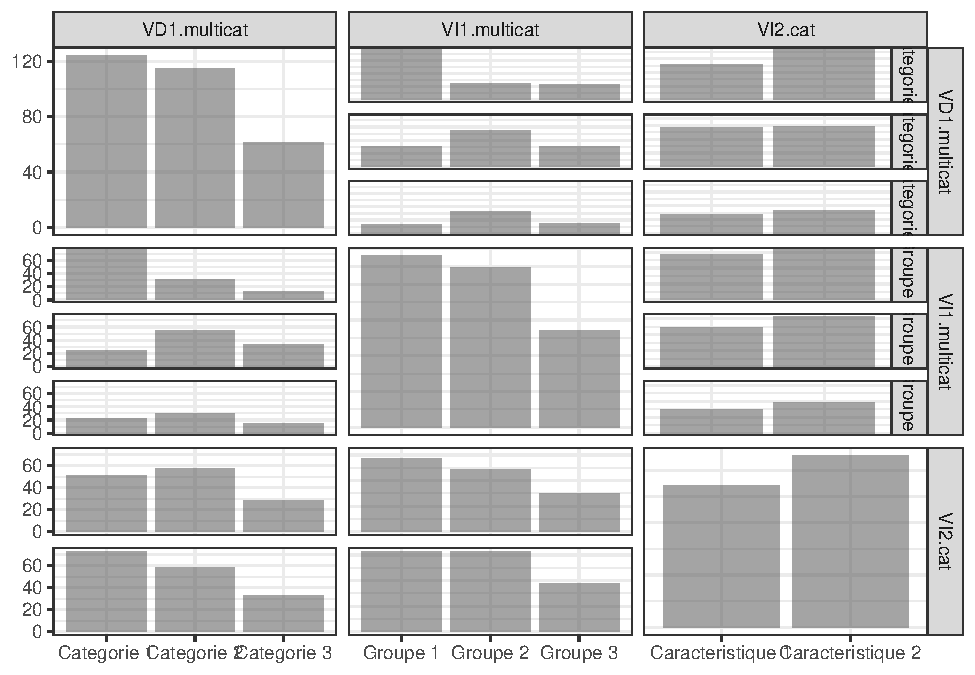
\includegraphics{Manuel_R_independant_files/figure-latex/unnamed-chunk-124-1.pdf}

\hypertarget{analyse-des-donnuxe9es-14}{%
\subsubsection{Analyse des données}\label{analyse-des-donnuxe9es-14}}

\begin{Shaded}
\begin{Highlighting}[]
\CommentTok{# calcul du test de log-linéaire  et stockage des résultats dans l’objet multinom2.test}
\NormalTok{regmultinom2.test <-}\StringTok{ }\KeywordTok{multinom}\NormalTok{(}\DataTypeTok{formula =}\NormalTok{ VD1.multicat  }\OperatorTok{~}\StringTok{ }\NormalTok{VI1.multicat }\OperatorTok{+}\StringTok{ }\NormalTok{VI2.cat, }
                    \DataTypeTok{data =}\NormalTok{ my_data.multinom2)}
\end{Highlighting}
\end{Shaded}

\begin{verbatim}
## # weights:  15 (8 variable)
## initial  value 329.583687 
## iter  10 value 293.652364
## final  value 293.604376 
## converged
\end{verbatim}

\begin{Shaded}
\begin{Highlighting}[]
\NormalTok{X2.regmultinom2 <-}\StringTok{ }\KeywordTok{as.numeric}\NormalTok{(}\KeywordTok{as.character}\NormalTok{(}\KeywordTok{Anova}\NormalTok{(regmultinom2.test)}\OperatorTok{$}\StringTok{'LR Chisq'}\NormalTok{))}
\NormalTok{p.regmultinom2 <-}\StringTok{ }\KeywordTok{as.numeric}\NormalTok{(}\KeywordTok{as.character}\NormalTok{(}\KeywordTok{Anova}\NormalTok{(regmultinom2.test)}\OperatorTok{$}\StringTok{'Pr(>Chisq)'}\NormalTok{))}

\CommentTok{# calcul des proportions de VD1.cat dans chaque modalité de VI1.cat}
\NormalTok{description.multinom2 <-}\StringTok{ }\NormalTok{my_data.multinom2 }\OperatorTok\StringTok{ }
\StringTok{  }\KeywordTok{group_by}\NormalTok{(VI1.multicat, VD1.multicat) }\OperatorTok
\StringTok{  }\KeywordTok{summarise}\NormalTok{(}\DataTypeTok{N =} \KeywordTok{n}\NormalTok{()) }\OperatorTok
\StringTok{  }\KeywordTok{mutate}\NormalTok{(}\DataTypeTok{proportion =}\NormalTok{ N }\OperatorTok{/}\StringTok{ }\KeywordTok{sum}\NormalTok{(N))}

\CommentTok{# tailles d'effet de VI1.cont sur VD1.multicat (odds ratio comparant l'effet de VI1.cont sur VD1.multicat entre les groupes 1 et 2 puis entre les groupes 1 et 3)}
\NormalTok{odds.ratio.regmultinom2 <-}\StringTok{ }\KeywordTok{exp}\NormalTok{(}\KeywordTok{coef}\NormalTok{(}\KeywordTok{summary}\NormalTok{(regmultinom2.test)))}

\NormalTok{posthoc.regmultinom2 <-}\StringTok{ }\KeywordTok{emmeans}\NormalTok{(regmultinom2.test, pairwise}\OperatorTok{~}\NormalTok{VD1.multicat}\OperatorTok{|}\NormalTok{VI1.multicat)}

\CommentTok{# Obtention des résultats de la régression logistique multinomiale évaluant l'effet global de VI1.cont sur VD1.cat }
\KeywordTok{data.frame}\NormalTok{(}\KeywordTok{cbind}\NormalTok{(}
  \DataTypeTok{Variable =} \StringTok{"VI1.multicat"}\NormalTok{, }
  \StringTok{"X2"}\NormalTok{ =}\StringTok{ }\NormalTok{X2.regmultinom2,}
  \StringTok{"p"}\NormalTok{ =}\StringTok{ }\NormalTok{p.regmultinom2))}
\end{Highlighting}
\end{Shaded}

\begin{verbatim}
##       Variable               X2                    p
## 1 VI1.multicat 45.0440877077601 3.89292187700322e-09
## 2 VI1.multicat 2.64905426287987    0.265928678673529
\end{verbatim}

\begin{Shaded}
\begin{Highlighting}[]
\CommentTok{# obtention du tableau de contigence et des proportions  }
\NormalTok{description.multinom2}
\end{Highlighting}
\end{Shaded}

\begin{verbatim}
## # A tibble: 9 x 4
## # Groups:   VI1.multicat [3]
##   VI1.multicat VD1.multicat     N proportion
##   <fct>        <fct>        <int>      <dbl>
## 1 Groupe 1     Categorie 1     76      0.633
## 2 Groupe 1     Categorie 2     31      0.258
## 3 Groupe 1     Categorie 3     13      0.108
## 4 Groupe 2     Categorie 1     25      0.223
## 5 Groupe 2     Categorie 2     54      0.482
## 6 Groupe 2     Categorie 3     33      0.295
## 7 Groupe 3     Categorie 1     23      0.338
## 8 Groupe 3     Categorie 2     30      0.441
## 9 Groupe 3     Categorie 3     15      0.221
\end{verbatim}

\begin{Shaded}
\begin{Highlighting}[]
\CommentTok{# Obtention des résultats du test de régression multinomiale}
\KeywordTok{Anova}\NormalTok{(regmultinom2.test)}
\end{Highlighting}
\end{Shaded}

\begin{verbatim}
## Analysis of Deviance Table (Type II tests)
## 
## Response: VD1.multicat
##              LR Chisq Df Pr(>Chisq)    
## VI1.multicat   45.044  4  3.893e-09 ***
## VI2.cat         2.649  2     0.2659    
## ---
## Signif. codes:  0 '***' 0.001 '**' 0.01 '*' 0.05 '.' 0.1 ' ' 1
\end{verbatim}

\begin{Shaded}
\begin{Highlighting}[]
\CommentTok{# obtention des tests post hoc }
\NormalTok{posthoc.regmultinom2}
\end{Highlighting}
\end{Shaded}

\begin{verbatim}
## $emmeans
## VI1.multicat = Groupe 1:
##  VD1.multicat  prob     SE df lower.CL upper.CL
##  Categorie 1  0.631 0.0439  8   0.5297    0.732
##  Categorie 2  0.260 0.0400  8   0.1680    0.353
##  Categorie 3  0.109 0.0285  8   0.0431    0.174
## 
## VI1.multicat = Groupe 2:
##  VD1.multicat  prob     SE df lower.CL upper.CL
##  Categorie 1  0.219 0.0388  8   0.1296    0.308
##  Categorie 2  0.486 0.0473  8   0.3772    0.595
##  Categorie 3  0.295 0.0433  8   0.1950    0.395
## 
## VI1.multicat = Groupe 3:
##  VD1.multicat  prob     SE df lower.CL upper.CL
##  Categorie 1  0.333 0.0568  8   0.2021    0.464
##  Categorie 2  0.446 0.0603  8   0.3069    0.585
##  Categorie 3  0.221 0.0505  8   0.1048    0.338
## 
## Results are averaged over the levels of: VI2.cat 
## Confidence level used: 0.95 
## 
## $contrasts
## VI1.multicat = Groupe 1:
##  contrast                  estimate     SE df t.ratio p.value
##  Categorie 1 - Categorie 2   0.3707 0.0791  8  4.689  0.0039 
##  Categorie 1 - Categorie 3   0.5222 0.0623  8  8.385  0.0001 
##  Categorie 2 - Categorie 3   0.1515 0.0538  8  2.815  0.0532 
## 
## VI1.multicat = Groupe 2:
##  contrast                  estimate     SE df t.ratio p.value
##  Categorie 1 - Categorie 2  -0.2673 0.0749  8 -3.568  0.0179 
##  Categorie 1 - Categorie 3  -0.0758 0.0672  8 -1.128  0.5249 
##  Categorie 2 - Categorie 3   0.1915 0.0819  8  2.337  0.1074 
## 
## VI1.multicat = Groupe 3:
##  contrast                  estimate     SE df t.ratio p.value
##  Categorie 1 - Categorie 2  -0.1128 0.1056  8 -1.068  0.5585 
##  Categorie 1 - Categorie 3   0.1118 0.0889  8  1.257  0.4558 
##  Categorie 2 - Categorie 3   0.2246 0.0956  8  2.350  0.1054 
## 
## Results are averaged over the levels of: VI2.cat 
## P value adjustment: tukey method for comparing a family of 3 estimates
\end{verbatim}

\begin{Shaded}
\begin{Highlighting}[]
\CommentTok{# obtention de la tailel d'effet}
\NormalTok{odds.ratio.regmultinom2}
\end{Highlighting}
\end{Shaded}

\begin{verbatim}
##             (Intercept) VI1.multicatGroupe 2 VI1.multicatGroupe 3
## Categorie 2   0.5113441             5.480052             3.289059
## Categorie 3   0.2018970             7.905919             3.889369
##             VI2.catCaracteristique 2
## Categorie 2                0.6401833
## Categorie 3                0.7283309
\end{verbatim}

\hypertarget{graphique-14}{%
\subsubsection{Graphique}\label{graphique-14}}

\begin{Shaded}
\begin{Highlighting}[]
\KeywordTok{ggplot}\NormalTok{(description.multinom2, }
       \KeywordTok{aes}\NormalTok{(}\DataTypeTok{x =}\NormalTok{ VI1.multicat, }\DataTypeTok{y=}\NormalTok{proportion, }\DataTypeTok{fill =}\NormalTok{ VD1.multicat)) }\OperatorTok{+}\StringTok{ }
\StringTok{  }\KeywordTok{geom_bar}\NormalTok{(}\DataTypeTok{stat =} \StringTok{"identity"}\NormalTok{, }\DataTypeTok{position =} \KeywordTok{position_dodge2}\NormalTok{(}\DataTypeTok{preserve =} \StringTok{"single"}\NormalTok{)) }\OperatorTok{+}\StringTok{ }
\StringTok{  }\KeywordTok{scale_fill_grey}\NormalTok{(}\DataTypeTok{start =} \FloatTok{0.8}\NormalTok{, }\DataTypeTok{end =} \FloatTok{0.4}\NormalTok{) }\OperatorTok{+}
\StringTok{  }\KeywordTok{ylab}\NormalTok{(}\StringTok{"Proportion"}\NormalTok{) }\OperatorTok{+}\StringTok{ }\KeywordTok{xlab}\NormalTok{(}\StringTok{"VI1.multicat"}\NormalTok{) }\OperatorTok{+}\StringTok{ }
\StringTok{  }\KeywordTok{theme_bw}\NormalTok{() }\OperatorTok{+}\StringTok{ }
\StringTok{  }\KeywordTok{theme}\NormalTok{(}\DataTypeTok{axis.title.y =} \KeywordTok{element_text}\NormalTok{(}\DataTypeTok{size =} \DecValTok{14}\NormalTok{, }\DataTypeTok{hjust =} \FloatTok{0.5}\NormalTok{, }\DataTypeTok{face =}\StringTok{"bold"}\NormalTok{), }
        \DataTypeTok{axis.title.x =} \KeywordTok{element_text}\NormalTok{(}\DataTypeTok{face =}\StringTok{"bold"}\NormalTok{, }\DataTypeTok{size =} \DecValTok{14}\NormalTok{, }\DataTypeTok{hjust =} \FloatTok{0.5}\NormalTok{))}
\end{Highlighting}
\end{Shaded}

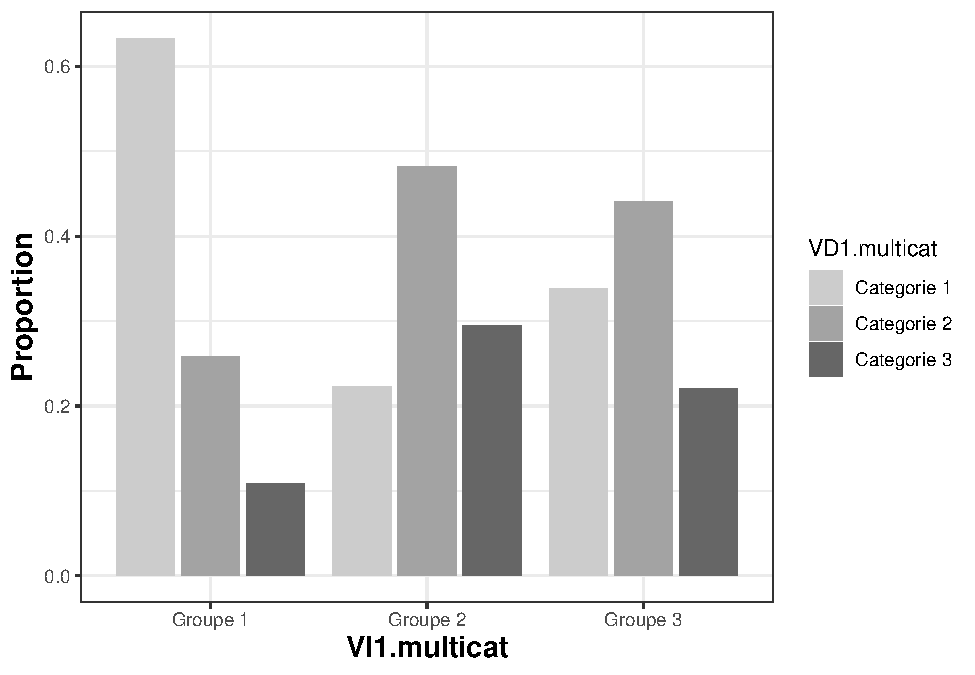
\includegraphics{Manuel_R_independant_files/figure-latex/unnamed-chunk-126-1.pdf}

\hypertarget{interpretation-14}{%
\subsubsection{Interpretation}\label{interpretation-14}}

{[}1{]} ``L'effet principal de VI1.multicat sur VD1.multicat atteint la significativite malgré l'ajustement par l'effet de VI2.cat (X² = 45.044, p = 4e-09). Au sein du groupe 1, la proportions d'individus en Catégorie 1 est plus élevée que la proportion d'individus en Catégorie 2 (p = 0.00394), elle-même marginalement plus élevée que la proportion d'individus en Catégorie 3 (p = 0.053). En revanche, au sein du groupe 2, seul le nombre d'individus en Catégorie 2 est plus élevé que le nombre d'individus en Catégorie 1 (p = 0.018). Pour le groupe 3 aucune différence significative n'était retrouvée (toutes valeurs p ajustées = 0.105).''

\hypertarget{ruxe9gression-logistique-multinomiale-3}{%
\subsection{Régression logistique multinomiale 3}\label{ruxe9gression-logistique-multinomiale-3}}

\hypertarget{type-de-variables-15}{%
\subsubsection{Type de variables}\label{type-de-variables-15}}

\textbf{Variable Dépendante :} Catégorielle (3 catégories ou +)
\textbf{Variables Indépendantes :} Numériques

\hypertarget{packages-nuxe9cessaires-15}{%
\subsubsection{Packages nécessaires}\label{packages-nuxe9cessaires-15}}

\begin{Shaded}
\begin{Highlighting}[]
\KeywordTok{library}\NormalTok{(ggplot2)}
\KeywordTok{library}\NormalTok{(GGally)}
\KeywordTok{library}\NormalTok{(effects)}
\KeywordTok{library}\NormalTok{(forcats)}
\KeywordTok{library}\NormalTok{(car)}
\KeywordTok{library}\NormalTok{(nnet)}
\KeywordTok{library}\NormalTok{(tidyr)}
\end{Highlighting}
\end{Shaded}

\hypertarget{donnuxe9es-ruxe9elles-15}{%
\subsubsection{Données réelles}\label{donnuxe9es-ruxe9elles-15}}

\begin{Shaded}
\begin{Highlighting}[]
\CommentTok{# choisissez la ligne appropriée au format de votre fichier de données. }

\CommentTok{# si vos données sont dans un fichier .txt}
\NormalTok{my_data.regmultinom3 <-}\StringTok{ }\KeywordTok{read.delim}\NormalTok{(}\KeywordTok{file.choose}\NormalTok{())}

\CommentTok{# si vos données sont dans un fichier .csv}
\NormalTok{my_data.regmultinom3 <-}\StringTok{ }\KeywordTok{read.csv}\NormalTok{(}\KeywordTok{file.choose}\NormalTok{())}

\CommentTok{# si vos données sont dans un fichier .xls / .xlsx}
\NormalTok{my_data.regmultinom3 <-}\StringTok{ }\KeywordTok{read_excel}\NormalTok{(}\KeywordTok{file.choose}\NormalTok{())}

\CommentTok{# une fois vos données chargées, vous pouvez renommer vos noms de colonnes afin qu'ils correspondent à ceux utilisés dans le code ci-dessous}
\CommentTok{# Si vous ne souhaitez pas renommer vos noms de colonnes, sautez cette étape mais adaptez le code des parties suivantes en lui indiquant les noms de colonnes de vos données.}

\CommentTok{# On crée une nouvelle colonne pour votre variable dépendante multicatégorielle (remplacez 'votre.nom.de.colonne' par le nom approprié)}
\NormalTok{my_data.regmultinom3}\OperatorTok{$}\NormalTok{VD1.multicat <-}\StringTok{ }\NormalTok{my_data.regmultinom3}\OperatorTok{$}\StringTok{'votre.nom.de.colonne'}

\CommentTok{# On crée une nouvelle colonne pour vos variables indépendantes continues (remplacez 'votre.nom.de.colonne' par les noms appropriés)}
\NormalTok{my_data.regmultinom3}\OperatorTok{$}\NormalTok{VI1.cont <-}\StringTok{ }\NormalTok{my_data.regmultinom3}\OperatorTok{$}\StringTok{'votre.nom.de.colonne'}
\NormalTok{my_data.regmultinom3}\OperatorTok{$}\NormalTok{VI2.cont <-}\StringTok{ }\NormalTok{my_data.regmultinom3}\OperatorTok{$}\StringTok{'votre.nom.de.colonne'}
\end{Highlighting}
\end{Shaded}

\hypertarget{donnuxe9es-fictives-15}{%
\subsubsection{Données fictives}\label{donnuxe9es-fictives-15}}

\begin{Shaded}
\begin{Highlighting}[]
\KeywordTok{set.seed}\NormalTok{(}\DecValTok{4321}\NormalTok{)}
\NormalTok{my_data.regmultinom3 <-}\StringTok{ }\KeywordTok{data.frame}\NormalTok{(}
  \DataTypeTok{VD1.multicat =} \KeywordTok{rbinom}\NormalTok{(}\DecValTok{330}\NormalTok{, }\DecValTok{2}\NormalTok{, }\FloatTok{0.5}\NormalTok{) }\OperatorTok{+}\StringTok{ }\DecValTok{1}\NormalTok{,}
  \DataTypeTok{VI1.cont =} \KeywordTok{rnorm}\NormalTok{(}\DecValTok{330}\NormalTok{),}
  \DataTypeTok{VI2.cont =} \KeywordTok{rnorm}\NormalTok{(}\DecValTok{330}\NormalTok{))}

\CommentTok{# On renomme les catégories de VD1.multicat pour que les résultats soient plus lisibles}
\NormalTok{my_data.regmultinom3}\OperatorTok{$}\NormalTok{VD1.multicat <-}\StringTok{ }\KeywordTok{fct_recode}\NormalTok{(}\KeywordTok{factor}\NormalTok{(my_data.regmultinom3}\OperatorTok{$}\NormalTok{VD1.multicat), }
                                            \StringTok{"Categorie 1"}\NormalTok{ =}\StringTok{ "1"}\NormalTok{, }
                                            \StringTok{"Categorie 2"}\NormalTok{ =}\StringTok{ "2"}\NormalTok{,}
                                            \StringTok{"Categorie 3"}\NormalTok{ =}\StringTok{ "3"}\NormalTok{) }
\end{Highlighting}
\end{Shaded}

\hypertarget{duxe9claration-du-type-de-variables-14}{%
\subsubsection{Déclaration du type de variables}\label{duxe9claration-du-type-de-variables-14}}

\begin{Shaded}
\begin{Highlighting}[]
\NormalTok{my_data.regmultinom3}\OperatorTok{$}\NormalTok{VD1.multicat <-}\StringTok{ }\KeywordTok{factor}\NormalTok{(my_data.regmultinom3}\OperatorTok{$}\NormalTok{VD1.multicat)}
\NormalTok{my_data.regmultinom3}\OperatorTok{$}\NormalTok{VI1.cont <-}\StringTok{ }\KeywordTok{as.numeric}\NormalTok{(}\KeywordTok{as.character}\NormalTok{(my_data.regmultinom3}\OperatorTok{$}\NormalTok{VI1.cont))}
\NormalTok{my_data.regmultinom3}\OperatorTok{$}\NormalTok{VI2.cont <-}\StringTok{ }\KeywordTok{as.numeric}\NormalTok{(}\KeywordTok{as.character}\NormalTok{(my_data.regmultinom3}\OperatorTok{$}\NormalTok{VI2.cont))}
\end{Highlighting}
\end{Shaded}

\hypertarget{inspection-des-donnuxe9es-14}{%
\subsubsection{Inspection des données}\label{inspection-des-donnuxe9es-14}}

\begin{Shaded}
\begin{Highlighting}[]
\CommentTok{## Les graphiques situés sur la diagonale représentent la distribution des variables}
\CommentTok{## Les graphiques (ou les valeurs de corrélation) situés au dessus et en dessous de la diagonale représentent l'association entre les différentes variables}
\KeywordTok{ggpairs}\NormalTok{(my_data.regmultinom3,}
        \DataTypeTok{lower =} \KeywordTok{list}\NormalTok{(}\DataTypeTok{continuous =} \KeywordTok{wrap}\NormalTok{(}\StringTok{"smooth"}\NormalTok{, }\DataTypeTok{alpha =} \FloatTok{0.7}\NormalTok{), }\DataTypeTok{combo =} \StringTok{"box_no_facet"}\NormalTok{),}
        \DataTypeTok{upper =} \KeywordTok{list}\NormalTok{(}\DataTypeTok{combo =} \StringTok{"facetdensity"}\NormalTok{, }\DataTypeTok{discrete =} \StringTok{"facetbar"}\NormalTok{), }
        \DataTypeTok{mapping =} \KeywordTok{aes}\NormalTok{(}\DataTypeTok{alpha =} \FloatTok{0.8}\NormalTok{)) }\OperatorTok{+}\StringTok{ }\KeywordTok{theme_bw}\NormalTok{()}
\end{Highlighting}
\end{Shaded}

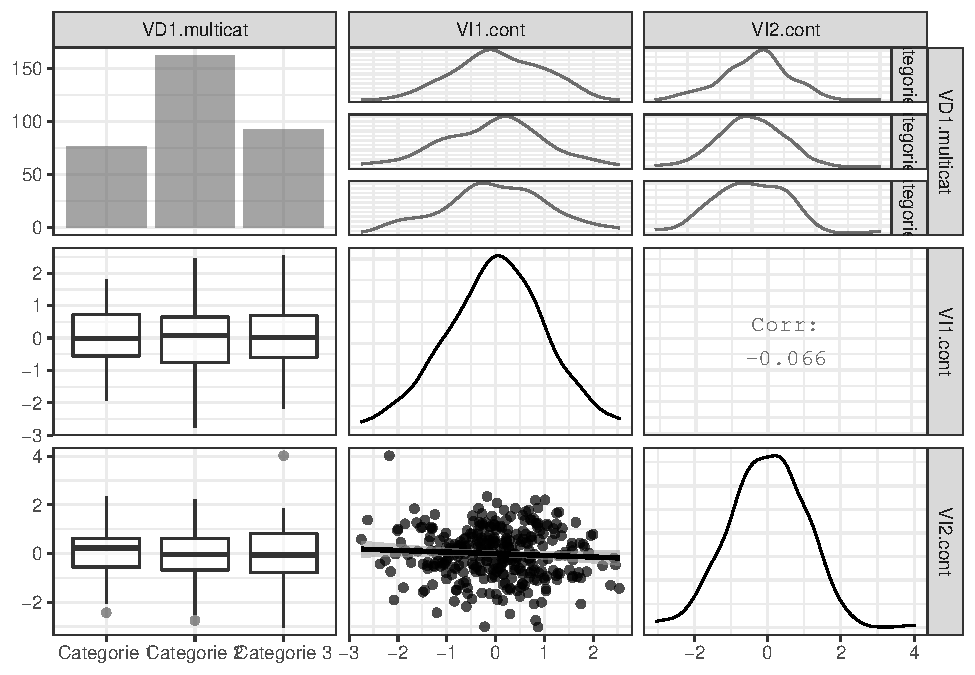
\includegraphics{Manuel_R_independant_files/figure-latex/unnamed-chunk-132-1.pdf}

\hypertarget{analyse-des-donnuxe9es-15}{%
\subsubsection{Analyse des données}\label{analyse-des-donnuxe9es-15}}

\begin{Shaded}
\begin{Highlighting}[]
\CommentTok{# calcul de la régression logistique multinomiale et stockage des résultats dans l’objet regmultinom3.test}
\NormalTok{regmultinom3.test <-}\StringTok{ }\KeywordTok{multinom}\NormalTok{(}\DataTypeTok{formula =}\NormalTok{ VD1.multicat }\OperatorTok{~}\StringTok{ }\NormalTok{VI1.cont }\OperatorTok{+}\StringTok{ }\NormalTok{VI2.cont, }
                              \DataTypeTok{data =}\NormalTok{ my_data.regmultinom3)}
\end{Highlighting}
\end{Shaded}

\begin{verbatim}
## # weights:  12 (6 variable)
## initial  value 362.542055 
## iter  10 value 343.124110
## final  value 343.124107 
## converged
\end{verbatim}

\begin{Shaded}
\begin{Highlighting}[]
\NormalTok{X2.regmultinom3 <-}\StringTok{ }\KeywordTok{as.numeric}\NormalTok{(}\KeywordTok{as.character}\NormalTok{(}\KeywordTok{Anova}\NormalTok{(regmultinom3.test)}\OperatorTok{$}\StringTok{'LR Chisq'}\NormalTok{))}
\NormalTok{p.regmultinom3 <-}\StringTok{ }\KeywordTok{as.numeric}\NormalTok{(}\KeywordTok{as.character}\NormalTok{(}\KeywordTok{Anova}\NormalTok{(regmultinom3.test)}\OperatorTok{$}\StringTok{'Pr(>Chisq)'}\NormalTok{))}

\CommentTok{# tests post hoc explorant l'effet de VD1.cont sur chaque modalité de VD1.multicat}
\NormalTok{posthoc.regmultinom3 <-}\StringTok{ }\KeywordTok{emtrends}\NormalTok{(regmultinom3.test, }
                                 \DataTypeTok{var =} \StringTok{"VI1.cont"}\NormalTok{, }\OperatorTok{~}\StringTok{ }\NormalTok{VD1.multicat)}


\CommentTok{# tailles d'effet de VI1.cont sur VD1.multicat (odds ratio comparant l'effet de VI1.cont sur VD1.multicat entre les groupes 1 et 2 puis entre les groupes 1 et 3)}
\NormalTok{odds.ratio.regmultinom3 <-}\StringTok{ }\KeywordTok{exp}\NormalTok{(}\KeywordTok{coef}\NormalTok{(}\KeywordTok{summary}\NormalTok{(regmultinom3.test)))}

\CommentTok{# Obtention des résultats de la régression logistique multinomiale évaluant l'effet global de VI1.cont sur VD1.cat }
\KeywordTok{data.frame}\NormalTok{(}\KeywordTok{cbind}\NormalTok{(}
  \DataTypeTok{Variable =} \KeywordTok{c}\NormalTok{(}\StringTok{"VI1.cont"}\NormalTok{, }\StringTok{"VI2.cont"}\NormalTok{),}
  \StringTok{"X2"}\NormalTok{ =}\StringTok{ }\NormalTok{X2.regmultinom3,}
  \StringTok{"p"}\NormalTok{ =}\StringTok{ }\NormalTok{p.regmultinom3))}
\end{Highlighting}
\end{Shaded}

\begin{verbatim}
##   Variable               X2                 p
## 1 VI1.cont 1.05878865026409 0.588961580899968
## 2 VI2.cont 1.54550290941927 0.461740859838403
\end{verbatim}

\begin{Shaded}
\begin{Highlighting}[]
\CommentTok{# obtention des tests post hoc :}

\CommentTok{## explorant l'effet de VD1.cont sur chaque modalité de VD1.multicat}
\KeywordTok{test}\NormalTok{(posthoc.regmultinom3, }\DataTypeTok{adjust =} \StringTok{"mvt"}\NormalTok{)}
\end{Highlighting}
\end{Shaded}

\begin{verbatim}
##  VD1.multicat VI1.cont.trend     SE df t.ratio p.value
##  Categorie 1         0.02008 0.0237  6  0.848  0.6878 
##  Categorie 2        -0.02658 0.0282  6 -0.944  0.6336 
##  Categorie 3         0.00651 0.0252  6  0.258  0.9641 
## 
## P value adjustment: mvt method for 3 tests
\end{verbatim}

\begin{Shaded}
\begin{Highlighting}[]
\CommentTok{##comparant l'effet de VI1.cont entre chaque modalité de VD1.multicat}
\KeywordTok{pairs}\NormalTok{(posthoc.regmultinom3)}
\end{Highlighting}
\end{Shaded}

\begin{verbatim}
##  contrast                  estimate     SE df t.ratio p.value
##  Categorie 1 - Categorie 2   0.0467 0.0455  6  1.026  0.5890 
##  Categorie 1 - Categorie 3   0.0136 0.0400  6  0.339  0.9392 
##  Categorie 2 - Categorie 3  -0.0331 0.0480  6 -0.690  0.7778 
## 
## P value adjustment: tukey method for comparing a family of 3 estimates
\end{verbatim}

\begin{Shaded}
\begin{Highlighting}[]
\CommentTok{# des tailles d'effet}
\NormalTok{odds.ratio.regmultinom3}
\end{Highlighting}
\end{Shaded}

\begin{verbatim}
##             (Intercept)  VI1.cont  VI2.cont
## Categorie 2    2.150149 0.8677836 0.8618484
## Categorie 3    1.220189 0.9375591 0.8394665
\end{verbatim}

\hypertarget{graphique-15}{%
\subsubsection{Graphique}\label{graphique-15}}

\begin{Shaded}
\begin{Highlighting}[]
\NormalTok{adjusted.slope.regmultinom3 <-}\StringTok{ }\KeywordTok{as.data.frame}\NormalTok{(}
  \KeywordTok{effect}\NormalTok{(}
    \DataTypeTok{term=}\StringTok{"VI1.cont"}\NormalTok{, }
    \DataTypeTok{mod =}\NormalTok{ regmultinom3.test))}

\NormalTok{adjusted.slope.regmultinom3.long <-}\StringTok{ }\NormalTok{adjusted.slope.regmultinom3 }\OperatorTok\StringTok{ }
\StringTok{    }\NormalTok{dplyr}\OperatorTok{::}\KeywordTok{select}\NormalTok{(VI1.cont, prob.Categorie}\FloatTok{.1}\NormalTok{,prob.Categorie}\FloatTok{.2}\NormalTok{,prob.Categorie}\FloatTok{.3}\NormalTok{) }\OperatorTok
\StringTok{    }\KeywordTok{pivot_longer}\NormalTok{(}\OperatorTok{-}\NormalTok{VI1.cont, }
        \DataTypeTok{names_to=}\StringTok{"var"}\NormalTok{,}
        \DataTypeTok{values_to=}\StringTok{"VD"}\NormalTok{)}

\NormalTok{adjusted.slope.regmultinom3.long}\OperatorTok{$}\NormalTok{var<-}\StringTok{ }\KeywordTok{fct_recode}\NormalTok{(adjusted.slope.regmultinom3.long}\OperatorTok{$}\NormalTok{var, }
           \StringTok{"Categorie 1"}\NormalTok{ =}\StringTok{ "prob.Categorie.1"}\NormalTok{, }
           \StringTok{"Categorie 2"}\NormalTok{ =}\StringTok{ "prob.Categorie.2"}\NormalTok{,}
           \StringTok{"Categorie 3"}\NormalTok{ =}\StringTok{ "prob.Categorie.3"}\NormalTok{)}


\KeywordTok{ggplot}\NormalTok{(adjusted.slope.regmultinom3.long) }\OperatorTok{+}\StringTok{ }
\StringTok{  }\KeywordTok{geom_line}\NormalTok{(}\KeywordTok{aes}\NormalTok{(}\DataTypeTok{x =}\NormalTok{ VI1.cont, }\DataTypeTok{y =}\NormalTok{ VD, }\DataTypeTok{color =}\NormalTok{ var),  }\DataTypeTok{size =} \DecValTok{1}\NormalTok{) }\OperatorTok{+}\StringTok{ }
\StringTok{  }\KeywordTok{facet_wrap}\NormalTok{(}\OperatorTok{~}\StringTok{ }\NormalTok{var) }\OperatorTok{+}
\StringTok{  }\KeywordTok{ylab}\NormalTok{(}\StringTok{"Probabilité"}\NormalTok{) }\OperatorTok{+}\StringTok{ }
\StringTok{  }\KeywordTok{xlab}\NormalTok{(}\StringTok{"VI1.cont"}\NormalTok{) }\OperatorTok{+}
\StringTok{  }\KeywordTok{theme_bw}\NormalTok{() }\OperatorTok{+}\StringTok{ }
\StringTok{  }\KeywordTok{theme}\NormalTok{(}\DataTypeTok{axis.title.y =} \KeywordTok{element_text}\NormalTok{(}\DataTypeTok{size =} \DecValTok{14}\NormalTok{, }\DataTypeTok{hjust =} \FloatTok{0.5}\NormalTok{, }\DataTypeTok{face=}\StringTok{"bold"}\NormalTok{), }
        \DataTypeTok{axis.title.x =} \KeywordTok{element_text}\NormalTok{(}\DataTypeTok{face=}\StringTok{"bold"}\NormalTok{, }\DataTypeTok{size =} \DecValTok{14}\NormalTok{, }\DataTypeTok{hjust =} \FloatTok{0.5}\NormalTok{)) }\OperatorTok{+}\StringTok{ }
\StringTok{  }\KeywordTok{guides}\NormalTok{(}\DataTypeTok{color=}\OtherTok{FALSE}\NormalTok{) }
\end{Highlighting}
\end{Shaded}

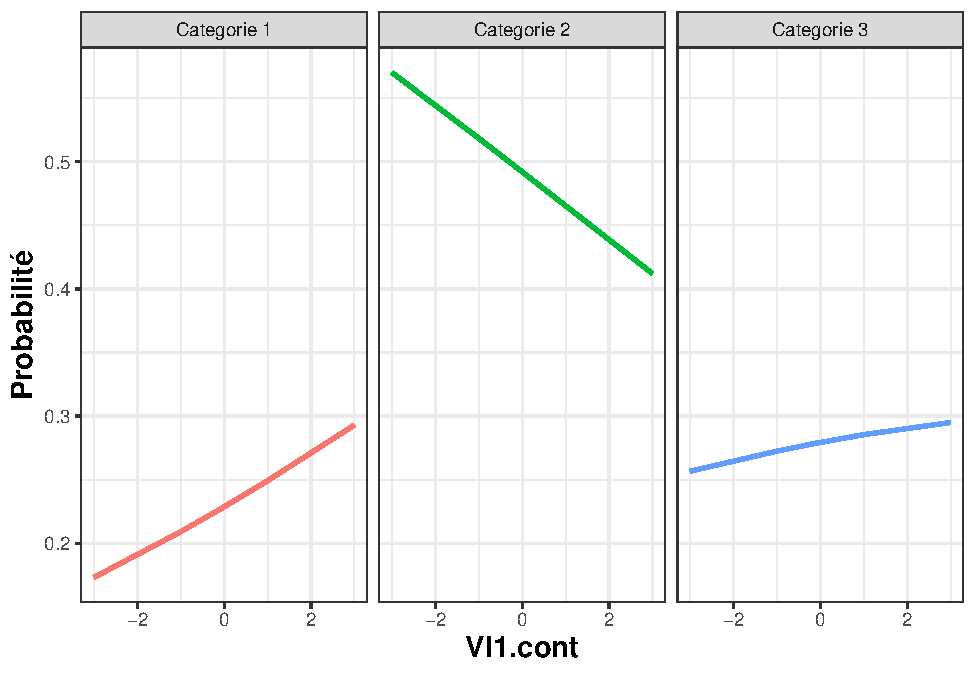
\includegraphics{Manuel_R_independant_files/figure-latex/unnamed-chunk-134-1.pdf}

\hypertarget{interpretation-15}{%
\subsubsection{Interpretation}\label{interpretation-15}}

{[}1{]} ``Les valeurs de VI1.cont ne sont pas liées à celles de VD1.multicat lorsque l'on ajuste par l'effet du VI2.cont (X² = 1.059, p = 0.58896). Plus précisement, quelle que soit la modalité de VD1.multicat, l'effet de VI1.cont n'est pas statistiquement significatif (valeur p ajustée \textgreater{} 0.634''

\hypertarget{ruxe9gression-logistique-multinomiale-4}{%
\subsection{Régression logistique multinomiale 4}\label{ruxe9gression-logistique-multinomiale-4}}

\hypertarget{type-de-variables-16}{%
\subsubsection{Type de variables}\label{type-de-variables-16}}

\textbf{Variable Dépendante :} Catégorielle (3 catégories ou +)
\textbf{Variables Indépendantes :} Numériques / Catégorielles

\hypertarget{packages-nuxe9cessaires-16}{%
\subsubsection{Packages nécessaires}\label{packages-nuxe9cessaires-16}}

\begin{Shaded}
\begin{Highlighting}[]
\KeywordTok{library}\NormalTok{(ggplot2)}
\KeywordTok{library}\NormalTok{(GGally)}
\KeywordTok{library}\NormalTok{(forcats)}
\KeywordTok{library}\NormalTok{(car)}
\KeywordTok{library}\NormalTok{(nnet)}
\KeywordTok{library}\NormalTok{(tidyr)}
\end{Highlighting}
\end{Shaded}

\hypertarget{donnuxe9es-ruxe9elles-16}{%
\subsubsection{Données réelles}\label{donnuxe9es-ruxe9elles-16}}

\begin{Shaded}
\begin{Highlighting}[]
\CommentTok{# choisissez la ligne appropriée au format de votre fichier de données. }

\CommentTok{# si vos données sont dans un fichier .txt}
\NormalTok{my_data.regmultinom4 <-}\StringTok{ }\KeywordTok{read.delim}\NormalTok{(}\KeywordTok{file.choose}\NormalTok{())}

\CommentTok{# si vos données sont dans un fichier .csv}
\NormalTok{my_data.regmultinom4 <-}\StringTok{ }\KeywordTok{read.csv}\NormalTok{(}\KeywordTok{file.choose}\NormalTok{())}

\CommentTok{# si vos données sont dans un fichier .xls / .xlsx}
\NormalTok{my_data.regmultinom4 <-}\StringTok{ }\KeywordTok{read_excel}\NormalTok{(}\KeywordTok{file.choose}\NormalTok{())}

\CommentTok{# une fois vos données chargées, vous pouvez renommer vos noms de colonnes afin qu'ils correspondent à ceux utilisés dans le code ci-dessous}
\CommentTok{# Si vous ne souhaitez pas renommer vos noms de colonnes, sautez cette étape mais adaptez le code des parties suivantes en lui indiquant les noms de colonnes de vos données.}

\CommentTok{# On crée une nouvelle colonne pour votre variable dépendante multicatégorielle (remplacez 'votre.nom.de.colonne' par le nom approprié)}
\NormalTok{my_data.regmultinom4}\OperatorTok{$}\NormalTok{VD1.multicat <-}\StringTok{ }\NormalTok{my_data.regmultinom4}\OperatorTok{$}\StringTok{'votre.nom.de.colonne'}

\CommentTok{# On crée une nouvelle colonne pour vos variables indépendantes continues (remplacez 'votre.nom.de.colonne' par les noms appropriés)}
\NormalTok{my_data.regmultinom4}\OperatorTok{$}\NormalTok{VI1.cont <-}\StringTok{ }\NormalTok{my_data.regmultinom4}\OperatorTok{$}\StringTok{'votre.nom.de.colonne'}
\NormalTok{my_data.regmultinom4}\OperatorTok{$}\NormalTok{VI2.cont <-}\StringTok{ }\NormalTok{my_data.regmultinom4}\OperatorTok{$}\StringTok{'votre.nom.de.colonne'}

\CommentTok{# On crée une nouvelle colonne pour votre variable catégorielle (remplacez 'votre.nom.de.colonne' par le nom approprié)}
\NormalTok{my_data.regmultinom4}\OperatorTok{$}\NormalTok{VI3.cat <-}\StringTok{ }\NormalTok{my_data.regmultinom4}\OperatorTok{$}\StringTok{'votre.nom.de.colonne'}
\end{Highlighting}
\end{Shaded}

\hypertarget{donnuxe9es-fictives-16}{%
\subsubsection{Données fictives}\label{donnuxe9es-fictives-16}}

\begin{Shaded}
\begin{Highlighting}[]
\KeywordTok{set.seed}\NormalTok{(}\DecValTok{4321}\NormalTok{)}
\NormalTok{my_data.regmultinom4 <-}\StringTok{ }\KeywordTok{data.frame}\NormalTok{(}
  \DataTypeTok{VD1.multicat =} \KeywordTok{rep}\NormalTok{(}\KeywordTok{c}\NormalTok{(}\DecValTok{1}\NormalTok{,}\DecValTok{2}\NormalTok{,}\DecValTok{3}\NormalTok{), }\DataTypeTok{each =} \DecValTok{40}\NormalTok{),}
  \DataTypeTok{VI1.cont =} \KeywordTok{c}\NormalTok{(}\KeywordTok{rnorm}\NormalTok{(}\DecValTok{40}\NormalTok{)}\OperatorTok{+}\FloatTok{0.35}\NormalTok{, }\KeywordTok{rnorm}\NormalTok{(}\DecValTok{40}\NormalTok{)}\OperatorTok{-}\FloatTok{0.35}\NormalTok{, }\KeywordTok{rnorm}\NormalTok{(}\DecValTok{40}\NormalTok{)}\OperatorTok{-}\FloatTok{0.35}\NormalTok{),}
  \DataTypeTok{VI2.cont =} \KeywordTok{rnorm}\NormalTok{(}\DecValTok{120}\NormalTok{),}
  \DataTypeTok{VI3.cat =} \KeywordTok{rbinom}\NormalTok{(}\DecValTok{120}\NormalTok{, }\DecValTok{1}\NormalTok{, }\FloatTok{.4}\NormalTok{) }\OperatorTok{+}\StringTok{ }\DecValTok{1}\NormalTok{)}

\CommentTok{# On renomme les catégories de VD1.multicat pour que les résultats soient plus lisibles}
\NormalTok{my_data.regmultinom4}\OperatorTok{$}\NormalTok{VD1.multicat <-}\StringTok{ }\KeywordTok{fct_recode}\NormalTok{(}\KeywordTok{factor}\NormalTok{(my_data.regmultinom4}\OperatorTok{$}\NormalTok{VD1.multicat), }
                                            \StringTok{"Categorie 1"}\NormalTok{ =}\StringTok{ "1"}\NormalTok{, }
                                            \StringTok{"Categorie 2"}\NormalTok{ =}\StringTok{ "2"}\NormalTok{,}
                                            \StringTok{"Categorie 3"}\NormalTok{ =}\StringTok{ "3"}\NormalTok{) }

\NormalTok{my_data.regmultinom4}\OperatorTok{$}\NormalTok{VI3.cat <-}\StringTok{ }\KeywordTok{fct_recode}\NormalTok{(}\KeywordTok{factor}\NormalTok{(my_data.regmultinom4}\OperatorTok{$}\NormalTok{VI3.cat), }
                                            \StringTok{"Caracteristique 1"}\NormalTok{ =}\StringTok{ "1"}\NormalTok{, }
                                            \StringTok{"Caracteristique 2"}\NormalTok{ =}\StringTok{ "2"}\NormalTok{) }
\end{Highlighting}
\end{Shaded}

\hypertarget{duxe9claration-du-type-de-variables-15}{%
\subsubsection{Déclaration du type de variables}\label{duxe9claration-du-type-de-variables-15}}

\begin{Shaded}
\begin{Highlighting}[]
\NormalTok{my_data.regmultinom4}\OperatorTok{$}\NormalTok{VD1.multicat <-}\StringTok{ }\KeywordTok{factor}\NormalTok{(my_data.regmultinom4}\OperatorTok{$}\NormalTok{VD1.multicat)}
\NormalTok{my_data.regmultinom4}\OperatorTok{$}\NormalTok{VI1.cont <-}\StringTok{ }\KeywordTok{as.numeric}\NormalTok{(}\KeywordTok{as.character}\NormalTok{(my_data.regmultinom4}\OperatorTok{$}\NormalTok{VI1.cont))}
\NormalTok{my_data.regmultinom4}\OperatorTok{$}\NormalTok{VI2.cont <-}\StringTok{ }\KeywordTok{as.numeric}\NormalTok{(}\KeywordTok{as.character}\NormalTok{(my_data.regmultinom4}\OperatorTok{$}\NormalTok{VI2.cont))}
\NormalTok{my_data.regmultinom4}\OperatorTok{$}\NormalTok{VI3.cat <-}\StringTok{ }\KeywordTok{factor}\NormalTok{(my_data.regmultinom4}\OperatorTok{$}\NormalTok{VI3.cat)}
\end{Highlighting}
\end{Shaded}

\hypertarget{inspection-des-donnuxe9es-15}{%
\subsubsection{Inspection des données}\label{inspection-des-donnuxe9es-15}}

\begin{Shaded}
\begin{Highlighting}[]
\CommentTok{## Les graphiques situés sur la diagonale représentent la distribution des variables}
\CommentTok{## Les graphiques (ou les valeurs de corrélation) situés au dessus et en dessous de la diagonale représentent l'association entre les différentes variables}
\KeywordTok{ggpairs}\NormalTok{(my_data.regmultinom4,}
        \DataTypeTok{lower =} \KeywordTok{list}\NormalTok{(}\DataTypeTok{continuous =} \KeywordTok{wrap}\NormalTok{(}\StringTok{"smooth"}\NormalTok{, }\DataTypeTok{alpha =} \FloatTok{0.7}\NormalTok{), }\DataTypeTok{combo =} \StringTok{"box_no_facet"}\NormalTok{),}
        \DataTypeTok{upper =} \KeywordTok{list}\NormalTok{(}\DataTypeTok{combo =} \StringTok{"facetdensity"}\NormalTok{, }\DataTypeTok{discrete =} \StringTok{"facetbar"}\NormalTok{), }
        \DataTypeTok{mapping =} \KeywordTok{aes}\NormalTok{(}\DataTypeTok{alpha =} \FloatTok{0.8}\NormalTok{)) }\OperatorTok{+}\StringTok{ }\KeywordTok{theme_bw}\NormalTok{()}
\end{Highlighting}
\end{Shaded}

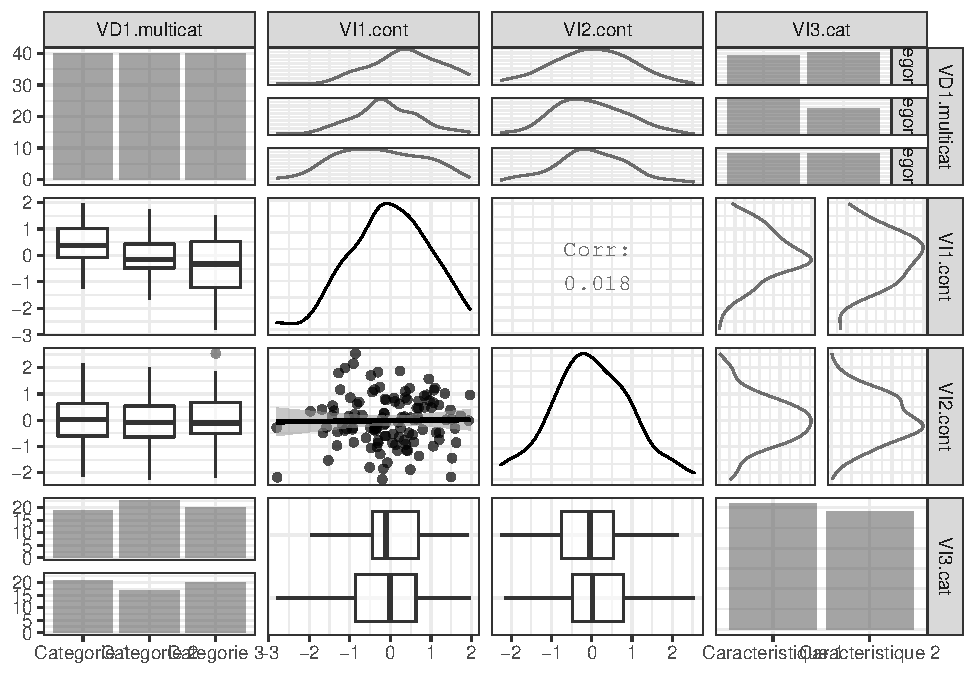
\includegraphics{Manuel_R_independant_files/figure-latex/unnamed-chunk-140-1.pdf}

\hypertarget{analyse-des-donnuxe9es-16}{%
\subsubsection{Analyse des données}\label{analyse-des-donnuxe9es-16}}

\begin{Shaded}
\begin{Highlighting}[]
\CommentTok{# calcul de la régression logistique multinomiale et stockage des résultats dans l’objet regmultinom4.test}
\NormalTok{regmultinom4.test <-}\StringTok{ }\KeywordTok{multinom}\NormalTok{(}\DataTypeTok{formula =}\NormalTok{ VD1.multicat }\OperatorTok{~}\StringTok{ }\NormalTok{VI1.cont }\OperatorTok{+}\StringTok{ }\NormalTok{VI2.cont }\OperatorTok{+}\StringTok{ }\NormalTok{VI3.cat, }
                              \DataTypeTok{data =}\NormalTok{ my_data.regmultinom4)}
\end{Highlighting}
\end{Shaded}

\begin{verbatim}
## # weights:  15 (8 variable)
## initial  value 131.833475 
## iter  10 value 124.324194
## final  value 124.309827 
## converged
\end{verbatim}

\begin{Shaded}
\begin{Highlighting}[]
\NormalTok{X2.regmultinom4 <-}\StringTok{ }\KeywordTok{as.numeric}\NormalTok{(}\KeywordTok{as.character}\NormalTok{(}\KeywordTok{Anova}\NormalTok{(regmultinom4.test)}\OperatorTok{$}\StringTok{'LR Chisq'}\NormalTok{))}
\NormalTok{p.regmultinom4 <-}\StringTok{ }\KeywordTok{as.numeric}\NormalTok{(}\KeywordTok{as.character}\NormalTok{(}\KeywordTok{Anova}\NormalTok{(regmultinom4.test)}\OperatorTok{$}\StringTok{'Pr(>Chisq)'}\NormalTok{))}

\CommentTok{# tests post hoc explorant l'effet de VD1.cont sur chaque modalité de VD1.multicat}
\NormalTok{posthoc.regmultinom4 <-}\StringTok{ }\KeywordTok{emtrends}\NormalTok{(regmultinom4.test, }
                                 \DataTypeTok{var =} \StringTok{"VI1.cont"}\NormalTok{, }\OperatorTok{~}\StringTok{ }\NormalTok{VD1.multicat)}


\CommentTok{# tailles d'effet de VI1.cont sur VD1.multicat (odds ratio comparant l'effet de VI1.cont sur VD1.multicat entre les groupes 1 et 2 puis entre les groupes 1 et 3)}
\NormalTok{odds.ratio.regmultinom4 <-}\StringTok{ }\KeywordTok{exp}\NormalTok{(}\KeywordTok{coef}\NormalTok{(}\KeywordTok{summary}\NormalTok{(regmultinom4.test)))}

\CommentTok{# Obtention des résultats de la régression logistique multinomiale évaluant l'effet global de VI1.cont sur VD1.cat }
\KeywordTok{data.frame}\NormalTok{(}\KeywordTok{cbind}\NormalTok{(}
  \DataTypeTok{Variable =} \KeywordTok{c}\NormalTok{(}\StringTok{"VI1.cont"}\NormalTok{, }\StringTok{"VI2.cont"}\NormalTok{, }\StringTok{"VI3.cat"}\NormalTok{),}
  \StringTok{"X2"}\NormalTok{ =}\StringTok{ }\NormalTok{X2.regmultinom4,}
  \StringTok{"p"}\NormalTok{ =}\StringTok{ }\NormalTok{p.regmultinom4))}
\end{Highlighting}
\end{Shaded}

\begin{verbatim}
##   Variable                 X2                    p
## 1 VI1.cont   14.1257841581388 0.000856298027825813
## 2 VI2.cont 0.0470392679264364    0.976754796912821
## 3  VI3.cat   1.02404809973623    0.599281375034191
\end{verbatim}

\begin{Shaded}
\begin{Highlighting}[]
\CommentTok{# obtention des tests post hoc :}

\CommentTok{## explorant l'effet de VD1.cont sur chaque modalité de VD1.multicat}
\KeywordTok{test}\NormalTok{(posthoc.regmultinom4, }\DataTypeTok{adjust =} \StringTok{"mvt"}\NormalTok{)}
\end{Highlighting}
\end{Shaded}

\begin{verbatim}
##  VD1.multicat VI1.cont.trend     SE df t.ratio p.value
##  Categorie 1          0.1727 0.0502  8  3.441  0.0214 
##  Categorie 2         -0.0446 0.0473  8 -0.943  0.6302 
##  Categorie 3         -0.1280 0.0480  8 -2.669  0.0659 
## 
## Results are averaged over the levels of: VI3.cat 
## P value adjustment: mvt method for 3 tests
\end{verbatim}

\begin{Shaded}
\begin{Highlighting}[]
\CommentTok{##comparant l'effet de VI1.cont entre chaque modalité de VD1.multicat}
\KeywordTok{pairs}\NormalTok{(posthoc.regmultinom4)}
\end{Highlighting}
\end{Shaded}

\begin{verbatim}
##  contrast                  estimate     SE df t.ratio p.value
##  Categorie 1 - Categorie 2   0.2173 0.0849  8 2.559   0.0776 
##  Categorie 1 - Categorie 3   0.3007 0.0860  8 3.495   0.0198 
##  Categorie 2 - Categorie 3   0.0834 0.0810  8 1.030   0.5800 
## 
## Results are averaged over the levels of: VI3.cat 
## P value adjustment: tukey method for comparing a family of 3 estimates
\end{verbatim}

\begin{Shaded}
\begin{Highlighting}[]
\CommentTok{# des tailles d'effet}
\NormalTok{odds.ratio.regmultinom4}
\end{Highlighting}
\end{Shaded}

\begin{verbatim}
##             (Intercept)  VI1.cont  VI2.cont VI3.catCaracteristique 2
## Categorie 2     1.38505 0.5075991 0.9521526                0.6244487
## Categorie 3     1.16946 0.3935861 0.9897427                0.7959744
\end{verbatim}

\hypertarget{graphique-16}{%
\subsubsection{Graphique}\label{graphique-16}}

\begin{Shaded}
\begin{Highlighting}[]
\NormalTok{adjusted.slope.regmultinom4 <-}\StringTok{ }\KeywordTok{as.data.frame}\NormalTok{(}
  \KeywordTok{effect}\NormalTok{(}
    \DataTypeTok{term=}\StringTok{"VI1.cont"}\NormalTok{, }
    \DataTypeTok{mod =}\NormalTok{ regmultinom4.test))}

\NormalTok{adjusted.slope.regmultinom4.long <-}\StringTok{ }\NormalTok{adjusted.slope.regmultinom4 }\OperatorTok\StringTok{ }
\StringTok{    }\NormalTok{dplyr}\OperatorTok{::}\KeywordTok{select}\NormalTok{(VI1.cont, prob.Categorie}\FloatTok{.1}\NormalTok{,prob.Categorie}\FloatTok{.2}\NormalTok{,prob.Categorie}\FloatTok{.3}\NormalTok{) }\OperatorTok
\StringTok{    }\KeywordTok{pivot_longer}\NormalTok{(}\OperatorTok{-}\NormalTok{VI1.cont, }
        \DataTypeTok{names_to=}\StringTok{"var"}\NormalTok{,}
        \DataTypeTok{values_to=}\StringTok{"VD"}\NormalTok{)}

\NormalTok{adjusted.slope.regmultinom4.long}\OperatorTok{$}\NormalTok{var<-}\StringTok{ }\KeywordTok{fct_recode}\NormalTok{(adjusted.slope.regmultinom4.long}\OperatorTok{$}\NormalTok{var, }
           \StringTok{"Categorie 1"}\NormalTok{ =}\StringTok{ "prob.Categorie.1"}\NormalTok{, }
           \StringTok{"Categorie 2"}\NormalTok{ =}\StringTok{ "prob.Categorie.2"}\NormalTok{,}
           \StringTok{"Categorie 3"}\NormalTok{ =}\StringTok{ "prob.Categorie.3"}\NormalTok{)}


\KeywordTok{ggplot}\NormalTok{(adjusted.slope.regmultinom4.long) }\OperatorTok{+}\StringTok{ }
\StringTok{  }\KeywordTok{geom_line}\NormalTok{(}\KeywordTok{aes}\NormalTok{(}\DataTypeTok{x =}\NormalTok{ VI1.cont, }\DataTypeTok{y =}\NormalTok{ VD, }\DataTypeTok{color =}\NormalTok{ var),  }\DataTypeTok{size =} \DecValTok{1}\NormalTok{) }\OperatorTok{+}\StringTok{ }
\StringTok{  }\KeywordTok{facet_wrap}\NormalTok{(}\OperatorTok{~}\StringTok{ }\NormalTok{var) }\OperatorTok{+}
\StringTok{  }\KeywordTok{ylab}\NormalTok{(}\StringTok{"Probabilité"}\NormalTok{) }\OperatorTok{+}\StringTok{ }
\StringTok{  }\KeywordTok{xlab}\NormalTok{(}\StringTok{"VI1.cont"}\NormalTok{) }\OperatorTok{+}
\StringTok{  }\KeywordTok{theme_bw}\NormalTok{() }\OperatorTok{+}\StringTok{ }
\StringTok{  }\KeywordTok{theme}\NormalTok{(}\DataTypeTok{axis.title.y =} \KeywordTok{element_text}\NormalTok{(}\DataTypeTok{size =} \DecValTok{14}\NormalTok{, }\DataTypeTok{hjust =} \FloatTok{0.5}\NormalTok{, }\DataTypeTok{face=}\StringTok{"bold"}\NormalTok{), }
        \DataTypeTok{axis.title.x =} \KeywordTok{element_text}\NormalTok{(}\DataTypeTok{face=}\StringTok{"bold"}\NormalTok{, }\DataTypeTok{size =} \DecValTok{14}\NormalTok{, }\DataTypeTok{hjust =} \FloatTok{0.5}\NormalTok{)) }\OperatorTok{+}\StringTok{ }
\StringTok{  }\KeywordTok{guides}\NormalTok{(}\DataTypeTok{color=}\OtherTok{FALSE}\NormalTok{) }
\end{Highlighting}
\end{Shaded}

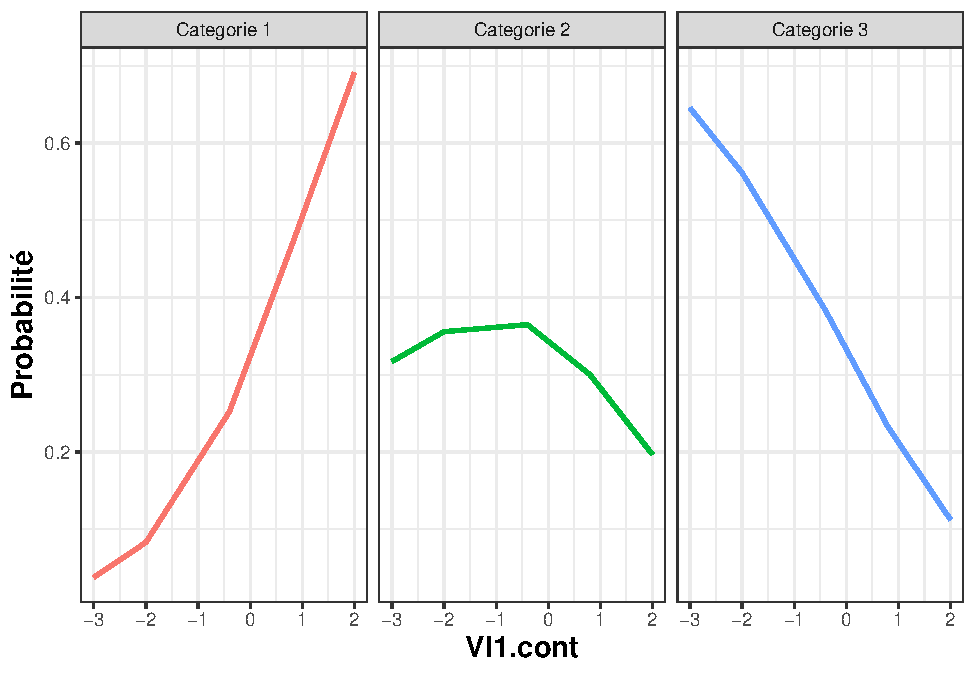
\includegraphics{Manuel_R_independant_files/figure-latex/unnamed-chunk-142-1.pdf}

\hypertarget{interpretation-16}{%
\subsubsection{Interpretation}\label{interpretation-16}}

{[}1{]} ``Les valeurs de VI1.cont sont liées à celles de VD1.multicat lorsque l'on ajuste par l'effet de VI2.cont et VI3.cat (X² = 14.126, p = 0.00086). Plus précisement, plus VI1.cont est élevée et plus la probabilité de Catégorie 1 augmente (valeur p ajustée = 0.022) et plus la probabilité de Catégorie 3 diminue (valeur p ajustée marginalement significative = 0.066). La probabilité de Catégorie 2 n'est pas liée à celle de VI1.cont (valeur p ajustée = 0.63). Concernant la différence entre les catégories de VD1.multicat, l'évolution des probabilités des Catégories 2 et 3 selon VI1.cont est différente de l'évolution de la probabilité de la Catégorie 1 (toutes valeurs p ajustées \textless{} 0.078)''

\hypertarget{ruxe9gression-logistique-ordinale-1}{%
\subsection{Régression logistique ordinale 1}\label{ruxe9gression-logistique-ordinale-1}}

\hypertarget{type-de-variables-17}{%
\subsubsection{Type de variables}\label{type-de-variables-17}}

\textbf{Variable Dépendante :} Ordinale (3 catégories ou +)
\textbf{Variables Indépendantes :} Catégorielles

\hypertarget{packages-nuxe9cessaires-17}{%
\subsubsection{Packages nécessaires}\label{packages-nuxe9cessaires-17}}

\begin{Shaded}
\begin{Highlighting}[]
\KeywordTok{library}\NormalTok{(ggplot2)}
\KeywordTok{library}\NormalTok{(GGally)}
\KeywordTok{library}\NormalTok{(forcats)}
\KeywordTok{library}\NormalTok{(dplyr)}
\KeywordTok{library}\NormalTok{(car)}
\KeywordTok{library}\NormalTok{(effects)}
\KeywordTok{library}\NormalTok{(tidyr)}
\KeywordTok{library}\NormalTok{(broom)}
\end{Highlighting}
\end{Shaded}

\hypertarget{donnuxe9es-ruxe9elles-17}{%
\subsubsection{Données réelles}\label{donnuxe9es-ruxe9elles-17}}

\begin{Shaded}
\begin{Highlighting}[]
\CommentTok{# choisissez la ligne appropriée au format de votre fichier de données. }

\CommentTok{# si vos données sont dans un fichier .txt}
\NormalTok{my_data.regord1 <-}\StringTok{ }\KeywordTok{read.delim}\NormalTok{(}\KeywordTok{file.choose}\NormalTok{())}

\CommentTok{# si vos données sont dans un fichier .csv}
\NormalTok{my_data.regord1 <-}\StringTok{ }\KeywordTok{read.csv}\NormalTok{(}\KeywordTok{file.choose}\NormalTok{())}

\CommentTok{# si vos données sont dans un fichier .xls / .xlsx}
\NormalTok{my_data.regord1 <-}\StringTok{ }\KeywordTok{read_excel}\NormalTok{(}\KeywordTok{file.choose}\NormalTok{())}

\CommentTok{# une fois vos données chargées, vous pouvez renommer vos noms de colonnes afin qu'ils correspondent à ceux utilisés dans le code ci-dessous}
\CommentTok{# Si vous ne souhaitez pas renommer vos noms de colonnes, sautez cette étape mais adaptez le code des parties suivantes en lui indiquant les noms de colonnes de vos données.}

\CommentTok{# On crée une nouvelle colonne pour votre variable dépendante ordinale (remplacez 'votre.nom.de.colonne' par le nom approprié)}
\NormalTok{my_data.regord1}\OperatorTok{$}\NormalTok{VD1.ord <-}\StringTok{ }\NormalTok{my_data.regord1}\OperatorTok{$}\StringTok{'votre.nom.de.colonne'}

\CommentTok{# On crée une nouvelle colonne pour votre variable indépendante catégorielle (remplacez 'votre.nom.de.colonne' par le nom approprié)}
\NormalTok{my_data.regord1}\OperatorTok{$}\NormalTok{VI1.cat <-}\StringTok{ }\NormalTok{my_data.regord1}\OperatorTok{$}\StringTok{'votre.nom.de.colonne'}
\end{Highlighting}
\end{Shaded}

\hypertarget{donnuxe9es-fictives-17}{%
\subsubsection{Données fictives}\label{donnuxe9es-fictives-17}}

\begin{Shaded}
\begin{Highlighting}[]
\KeywordTok{set.seed}\NormalTok{(}\DecValTok{4321}\NormalTok{)}
\NormalTok{regord1 <-}\StringTok{ }\KeywordTok{rbinom}\NormalTok{(}\DecValTok{200}\NormalTok{, }\DecValTok{1}\NormalTok{, }\FloatTok{0.8}\NormalTok{)}
\NormalTok{my_data.regord1 <-}\StringTok{ }\KeywordTok{data.frame}\NormalTok{(}
  \DataTypeTok{VD1.ord =}\NormalTok{ (}\KeywordTok{rbinom}\NormalTok{(}\DecValTok{200}\NormalTok{, }\DecValTok{2}\NormalTok{, }\FloatTok{0.5}\NormalTok{)}\OperatorTok{*}\NormalTok{regord1 }\OperatorTok{+}\StringTok{ }\DecValTok{1}\NormalTok{),}
  \DataTypeTok{VI1.cat =}\NormalTok{ (}\KeywordTok{rbinom}\NormalTok{(}\DecValTok{200}\NormalTok{, }\DecValTok{1}\NormalTok{, }\FloatTok{0.6}\NormalTok{)}\OperatorTok{*}\NormalTok{regord1 }\OperatorTok{+}\StringTok{ }\DecValTok{1}\NormalTok{))}

\CommentTok{# on recode les catégories de VD1.ord et VI1.cat pour que les résultats soient plus lisibles}
\NormalTok{my_data.regord1}\OperatorTok{$}\NormalTok{VI1.cat <-}\StringTok{ }\KeywordTok{fct_recode}\NormalTok{(}\KeywordTok{factor}\NormalTok{(my_data.regord1}\OperatorTok{$}\NormalTok{VI1.cat), }
                                    \StringTok{"Groupe 1"}\NormalTok{ =}\StringTok{ "1"}\NormalTok{, }
                                    \StringTok{"Groupe 2"}\NormalTok{ =}\StringTok{ "2"}\NormalTok{) }

\NormalTok{ my_data.regord1}\OperatorTok{$}\NormalTok{VD1.ord <-}\StringTok{ }\KeywordTok{fct_recode}\NormalTok{(}\KeywordTok{ordered}\NormalTok{(my_data.regord1}\OperatorTok{$}\NormalTok{VD1.ord), }
                                     \StringTok{"Faible"}\NormalTok{ =}\StringTok{ "1"}\NormalTok{, }
                                     \StringTok{"Modere"}\NormalTok{ =}\StringTok{ "2"}\NormalTok{,}
                                     \StringTok{"Severe"}\NormalTok{ =}\StringTok{ "3"}\NormalTok{) }
\end{Highlighting}
\end{Shaded}

\hypertarget{duxe9claration-du-type-de-variables-16}{%
\subsubsection{Déclaration du type de variables}\label{duxe9claration-du-type-de-variables-16}}

\begin{Shaded}
\begin{Highlighting}[]
\NormalTok{my_data.regord1}\OperatorTok{$}\NormalTok{VD1.ord <-}\StringTok{ }\KeywordTok{ordered}\NormalTok{(my_data.regord1}\OperatorTok{$}\NormalTok{VD1.ord, }
                                   \DataTypeTok{levels =} \KeywordTok{c}\NormalTok{(}\StringTok{"Faible"}\NormalTok{, }\StringTok{"Modere"}\NormalTok{, }\StringTok{"Severe"}\NormalTok{))}
\NormalTok{my_data.regord1}\OperatorTok{$}\NormalTok{VI1.cat <-}\StringTok{ }\KeywordTok{factor}\NormalTok{(my_data.regord1}\OperatorTok{$}\NormalTok{VI1.cat)}
\end{Highlighting}
\end{Shaded}

\hypertarget{inspection-des-donnuxe9es-16}{%
\subsubsection{Inspection des données}\label{inspection-des-donnuxe9es-16}}

\begin{Shaded}
\begin{Highlighting}[]
\CommentTok{## Les graphiques situés sur la diagonale représentent la distribution des variables}
\CommentTok{## Les graphiques (ou les valeurs de corrélation) situés au dessus et en dessous de la diagonale représentent l'association entre les différentes variables}
\KeywordTok{ggpairs}\NormalTok{(my_data.regord1,}
        \DataTypeTok{lower =} \KeywordTok{list}\NormalTok{(}\DataTypeTok{continuous =} \KeywordTok{wrap}\NormalTok{(}\StringTok{"smooth"}\NormalTok{, }\DataTypeTok{alpha =} \FloatTok{0.7}\NormalTok{), }\DataTypeTok{combo =} \StringTok{"box_no_facet"}\NormalTok{),}
        \DataTypeTok{upper =} \KeywordTok{list}\NormalTok{(}\DataTypeTok{combo =} \StringTok{"facetdensity"}\NormalTok{, }\DataTypeTok{discrete =} \StringTok{"facetbar"}\NormalTok{), }
        \DataTypeTok{mapping =} \KeywordTok{aes}\NormalTok{(}\DataTypeTok{alpha =} \FloatTok{0.8}\NormalTok{)) }\OperatorTok{+}\StringTok{ }\KeywordTok{theme_bw}\NormalTok{()}
\end{Highlighting}
\end{Shaded}

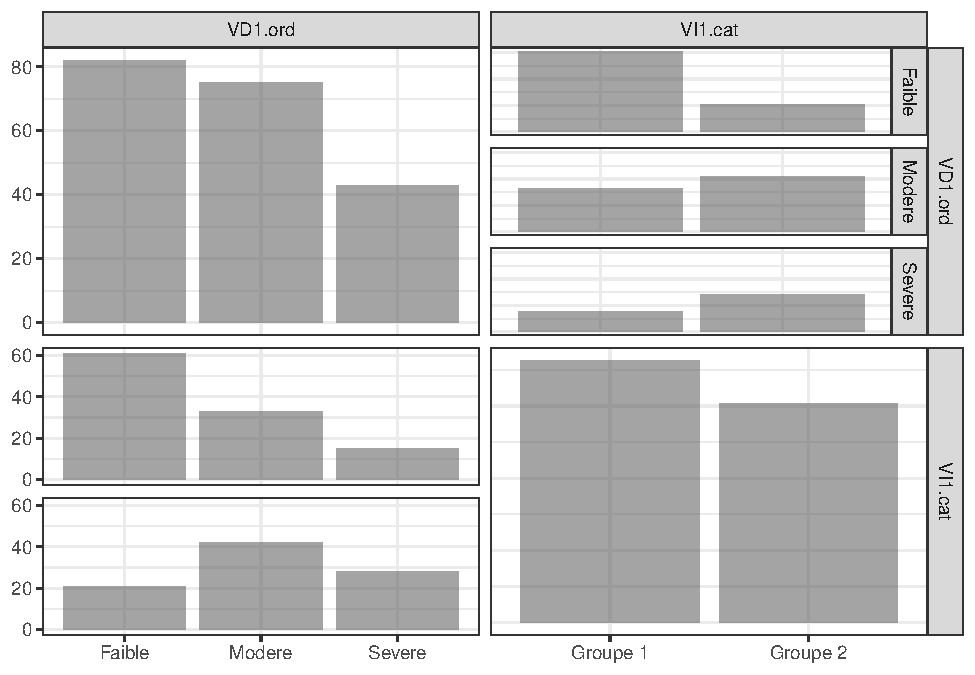
\includegraphics{Manuel_R_independant_files/figure-latex/unnamed-chunk-148-1.pdf}

\hypertarget{analyse-des-donnuxe9es-17}{%
\subsubsection{Analyse des données}\label{analyse-des-donnuxe9es-17}}

\begin{Shaded}
\begin{Highlighting}[]
\CommentTok{# Pour vérifier que vos catégories de VD1.ord ont bien été hierarchisées correctement}
\KeywordTok{str}\NormalTok{(my_data.regord1}\OperatorTok{$}\NormalTok{VD1.ord)}
\end{Highlighting}
\end{Shaded}

\begin{verbatim}
##  Ord.factor w/ 3 levels "Faible"<"Modere"<..: 3 1 2 2 1 2 2 1 3 2 ...
\end{verbatim}

\begin{Shaded}
\begin{Highlighting}[]
\CommentTok{# calcul de la régression ordinale et stockage des résultats dans l’objet regord1.test}
\NormalTok{regord1.test <-}\StringTok{ }\NormalTok{MASS}\OperatorTok{::}\KeywordTok{polr}\NormalTok{(}\DataTypeTok{formula =}\NormalTok{ VD1.ord }\OperatorTok{~}\StringTok{ }\NormalTok{VI1.cat, }
                           \DataTypeTok{data =}\NormalTok{ my_data.regord1)}

\CommentTok{# Anova(MASS::polr(formula = VD1.ord.ON ~ VI1.cat, data = my_data.regord1))}
\CommentTok{# wilcox.test(VD1.ord ~ VI1.cat, data = my_data.regord1)}

\CommentTok{# calcul de la taille d'effet de VI1.cat sur VD1.ord (odds ratio)}
\NormalTok{oddsratio.regord1 <-}\StringTok{ }\KeywordTok{exp}\NormalTok{(}\KeywordTok{coef}\NormalTok{(}\KeywordTok{summary}\NormalTok{(regord1.test)))}

\CommentTok{# Obtention des résultats de la regression ordinale}
\KeywordTok{Anova}\NormalTok{(regord1.test)}
\end{Highlighting}
\end{Shaded}

\begin{verbatim}
## Analysis of Deviance Table (Type II tests)
## 
## Response: VD1.ord
##         LR Chisq Df Pr(>Chisq)    
## VI1.cat   22.569  1  2.027e-06 ***
## ---
## Signif. codes:  0 '***' 0.001 '**' 0.01 '*' 0.05 '.' 0.1 ' ' 1
\end{verbatim}

\begin{Shaded}
\begin{Highlighting}[]
\CommentTok{# Obtention de la taille d'effet}
\NormalTok{oddsratio.regord1}
\end{Highlighting}
\end{Shaded}

\begin{verbatim}
##                    Value Std. Error     t value
## VI1.catGroupe 2 3.633876   1.320968  103.057160
## Faible|Modere   1.219093   1.210530    2.820439
## Modere|Severe   7.510103   1.276284 3885.198214
\end{verbatim}

\hypertarget{graphique-17}{%
\subsubsection{Graphique}\label{graphique-17}}

\begin{Shaded}
\begin{Highlighting}[]
\NormalTok{crude.slope.regord1 <-}\StringTok{ }\KeywordTok{as.data.frame}\NormalTok{(}
  \KeywordTok{effect}\NormalTok{(}
    \DataTypeTok{term=}\StringTok{"VI1.cat"}\NormalTok{, }
    \DataTypeTok{mod =}\NormalTok{ regord1.test))}

\NormalTok{crude.slope.regord1.long.prob <-}\StringTok{ }\NormalTok{crude.slope.regord1 }\OperatorTok\StringTok{ }
\StringTok{    }\NormalTok{dplyr}\OperatorTok{::}\KeywordTok{select}\NormalTok{(VI1.cat, }
\NormalTok{                  prob.Faible,}
\NormalTok{                  prob.Modere,}
\NormalTok{                  prob.Severe) }\OperatorTok
\StringTok{    }\KeywordTok{pivot_longer}\NormalTok{(}\OperatorTok{-}\NormalTok{VI1.cat, }
        \DataTypeTok{names_to=}\StringTok{"VD1.ord"}\NormalTok{,}
        \DataTypeTok{values_to=}\StringTok{"VD"}\NormalTok{)}

\NormalTok{crude.slope.regord1.long.se <-}\StringTok{ }\NormalTok{crude.slope.regord1 }\OperatorTok\StringTok{ }
\StringTok{    }\NormalTok{dplyr}\OperatorTok{::}\KeywordTok{select}\NormalTok{(VI1.cat, }
\NormalTok{                  se.prob.Faible,}
\NormalTok{                  se.prob.Modere,}
\NormalTok{                  se.prob.Severe) }\OperatorTok
\StringTok{    }\KeywordTok{pivot_longer}\NormalTok{(}\OperatorTok{-}\NormalTok{VI1.cat, }
        \DataTypeTok{names_to=}\StringTok{"VD1.ord.se"}\NormalTok{,}
        \DataTypeTok{values_to=}\StringTok{"SE"}\NormalTok{)}

\NormalTok{crude.slope.regord1.long <-}\StringTok{ }\KeywordTok{cbind}\NormalTok{(crude.slope.regord1.long.prob,                                    crude.slope.regord1.long.se[,}\KeywordTok{c}\NormalTok{(}\StringTok{'VD1.ord.se'}\NormalTok{, }\StringTok{'SE'}\NormalTok{)])}

\NormalTok{crude.slope.regord1.long}\OperatorTok{$}\NormalTok{VD1.ord<-}\StringTok{ }\KeywordTok{fct_recode}\NormalTok{(crude.slope.regord1.long}\OperatorTok{$}\NormalTok{VD1.ord,}
    \StringTok{"Faible"}\NormalTok{ =}\StringTok{ "prob.Faible"}\NormalTok{, }
    \StringTok{"Modere"}\NormalTok{ =}\StringTok{ "prob.Modere"}\NormalTok{,}
    \StringTok{"Severe"}\NormalTok{ =}\StringTok{ "prob.Severe"}\NormalTok{)}

\NormalTok{crude.slope.regord1.long}\OperatorTok{$}\NormalTok{VD1.ord <-}\StringTok{ }\KeywordTok{ordered}\NormalTok{(crude.slope.regord1.long}\OperatorTok{$}\NormalTok{VD1.ord, }
        \DataTypeTok{levels =} \KeywordTok{c}\NormalTok{(}\StringTok{"Faible"}\NormalTok{, }\StringTok{"Modere"}\NormalTok{, }\StringTok{"Severe"}\NormalTok{))}

\KeywordTok{ggplot}\NormalTok{(crude.slope.regord1.long, }
       \KeywordTok{aes}\NormalTok{(}\DataTypeTok{x =}\NormalTok{ VI1.cat, }\DataTypeTok{y =}\NormalTok{ VD, }\DataTypeTok{color =}\NormalTok{ VD1.ord)) }\OperatorTok{+}\StringTok{ }
\StringTok{  }\KeywordTok{geom_errorbar}\NormalTok{(}\KeywordTok{aes}\NormalTok{(}
      \DataTypeTok{ymin =}\NormalTok{ VD }\OperatorTok{-}\StringTok{ }\NormalTok{SE,}
      \DataTypeTok{ymax =}\NormalTok{ VD }\OperatorTok{+}\StringTok{ }\NormalTok{SE),}
      \DataTypeTok{width =} \DecValTok{0}\NormalTok{, }\DataTypeTok{position =} \KeywordTok{position_dodge}\NormalTok{(}\FloatTok{0.3}\NormalTok{)) }\OperatorTok{+}
\StringTok{  }\KeywordTok{geom_point}\NormalTok{(}\DataTypeTok{size =} \DecValTok{2}\NormalTok{, }\DataTypeTok{position =} \KeywordTok{position_dodge}\NormalTok{(}\FloatTok{0.3}\NormalTok{)) }\OperatorTok{+}
\StringTok{  }\KeywordTok{ylab}\NormalTok{(}\StringTok{"Probabilité"}\NormalTok{) }\OperatorTok{+}\StringTok{ }\KeywordTok{xlab}\NormalTok{(}\StringTok{"VI1.cat"}\NormalTok{) }\OperatorTok{+}
\StringTok{  }\KeywordTok{theme_bw}\NormalTok{() }\OperatorTok{+}\StringTok{ }
\StringTok{  }\KeywordTok{theme}\NormalTok{(}
    \DataTypeTok{axis.title.y =} \KeywordTok{element_text}\NormalTok{(}\DataTypeTok{size =} \DecValTok{14}\NormalTok{, }\DataTypeTok{hjust =} \FloatTok{0.5}\NormalTok{, }\DataTypeTok{face =}\StringTok{"bold"}\NormalTok{), }
    \DataTypeTok{axis.title.x =} \KeywordTok{element_text}\NormalTok{(}\DataTypeTok{face =}\StringTok{"bold"}\NormalTok{, }\DataTypeTok{size =} \DecValTok{14}\NormalTok{, }\DataTypeTok{hjust =} \FloatTok{0.5}\NormalTok{)) }\OperatorTok{+}\StringTok{ }
\StringTok{  }\KeywordTok{scale_color_grey}\NormalTok{(}\DataTypeTok{start=}\FloatTok{0.7}\NormalTok{, }\DataTypeTok{end=}\FloatTok{0.01}\NormalTok{) }\OperatorTok{+}\StringTok{ }
\StringTok{  }\KeywordTok{scale_y_continuous}\NormalTok{(}\DataTypeTok{limits=}\KeywordTok{c}\NormalTok{(}\DecValTok{0}\NormalTok{,}\DecValTok{1}\NormalTok{))}
\end{Highlighting}
\end{Shaded}

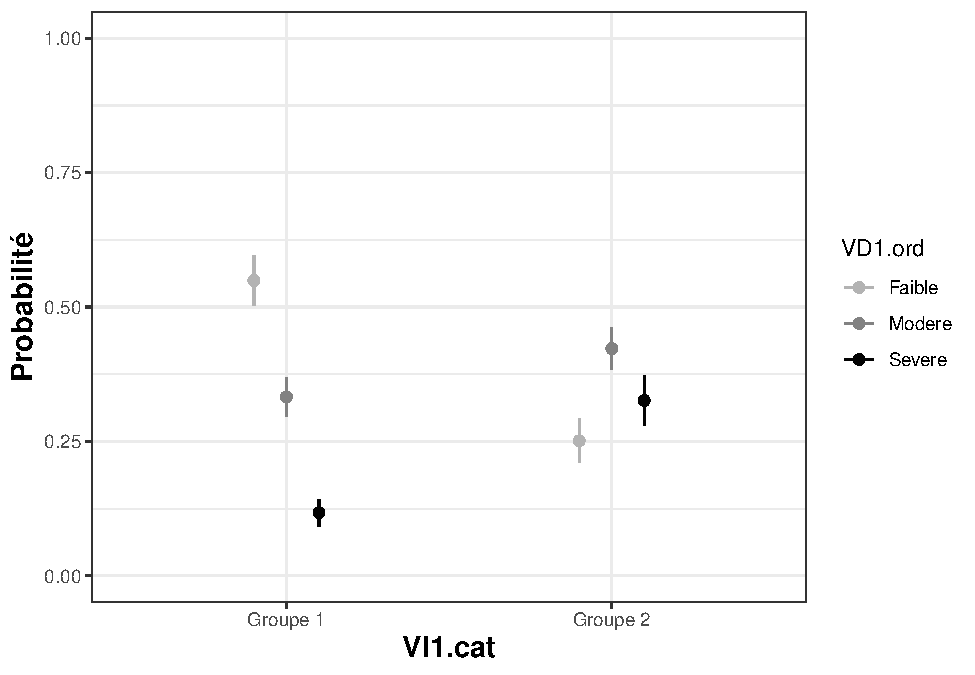
\includegraphics{Manuel_R_independant_files/figure-latex/unnamed-chunk-150-1.pdf}

\hypertarget{interpretation-17}{%
\subsubsection{Interpretation}\label{interpretation-17}}

{[}1{]} ``La probabilité d'obtenir un score faible à VD1.ord (comparativement à un score modéré ou sévère) est plus importante dans le groupe 1 que dans le groupe 2 (X² = 22.569, Odds ratio = 3.634, p = 2e-06).''

\hypertarget{ruxe9gression-logistique-ordinale-2}{%
\subsection{Régression logistique ordinale 2}\label{ruxe9gression-logistique-ordinale-2}}

\hypertarget{type-de-variables-18}{%
\subsubsection{Type de variables}\label{type-de-variables-18}}

\textbf{Variable Dépendante :} Ordinale (3 catégories ou +)
\textbf{Variables Indépendantes:} Numériques

\hypertarget{packages-nuxe9cessaires-18}{%
\subsubsection{Packages nécessaires}\label{packages-nuxe9cessaires-18}}

\begin{Shaded}
\begin{Highlighting}[]
\KeywordTok{library}\NormalTok{(ggplot2)}
\KeywordTok{library}\NormalTok{(GGally)}
\KeywordTok{library}\NormalTok{(forcats)}
\KeywordTok{library}\NormalTok{(dplyr)}
\KeywordTok{library}\NormalTok{(car)}
\KeywordTok{library}\NormalTok{(effects)}
\KeywordTok{library}\NormalTok{(tidyr)}
\KeywordTok{library}\NormalTok{(broom)}
\end{Highlighting}
\end{Shaded}

\hypertarget{donnuxe9es-ruxe9elles-18}{%
\subsubsection{Données réelles}\label{donnuxe9es-ruxe9elles-18}}

\begin{Shaded}
\begin{Highlighting}[]
\CommentTok{# choisissez la ligne appropriée au format de votre fichier de données. }

\CommentTok{# si vos données sont dans un fichier .txt}
\NormalTok{my_data.regord2 <-}\StringTok{ }\KeywordTok{read.delim}\NormalTok{(}\KeywordTok{file.choose}\NormalTok{())}

\CommentTok{# si vos données sont dans un fichier .csv}
\NormalTok{my_data.regord2 <-}\StringTok{ }\KeywordTok{read.csv}\NormalTok{(}\KeywordTok{file.choose}\NormalTok{())}

\CommentTok{# si vos données sont dans un fichier .xls / .xlsx}
\NormalTok{my_data.regord2 <-}\StringTok{ }\KeywordTok{read_excel}\NormalTok{(}\KeywordTok{file.choose}\NormalTok{())}

\CommentTok{# une fois vos données chargées, vous pouvez renommer vos noms de colonnes afin qu'ils correspondent à ceux utilisés dans le code ci-dessous}
\CommentTok{# Si vous ne souhaitez pas renommer vos noms de colonnes, sautez cette étape mais adaptez le code des parties suivantes en lui indiquant les noms de colonnes de vos données.}

\CommentTok{# On crée une nouvelle colonne pour votre variable dépendante ordinale (remplacez 'votre.nom.de.colonne' par le nom approprié)}
\NormalTok{my_data.regord2}\OperatorTok{$}\NormalTok{VD1.ord <-}\StringTok{ }\NormalTok{my_data.regord2}\OperatorTok{$}\StringTok{'votre.nom.de.colonne'}

\CommentTok{# On crée une nouvelle colonne pour votre variable indépendante continue (remplacez 'votre.nom.de.colonne' par le nom approprié)}
\NormalTok{my_data.regord2}\OperatorTok{$}\NormalTok{VI1.cont <-}\StringTok{ }\NormalTok{my_data.regord2}\OperatorTok{$}\StringTok{'votre.nom.de.colonne'}
\end{Highlighting}
\end{Shaded}

\hypertarget{donnuxe9es-fictives-18}{%
\subsubsection{Données fictives}\label{donnuxe9es-fictives-18}}

\begin{Shaded}
\begin{Highlighting}[]
\KeywordTok{set.seed}\NormalTok{(}\DecValTok{4321}\NormalTok{)}
\NormalTok{my_data.regord2 <-}\StringTok{ }\KeywordTok{data.frame}\NormalTok{(}
  \DataTypeTok{VD1.ord =} \KeywordTok{rep}\NormalTok{(}\KeywordTok{c}\NormalTok{(}\DecValTok{1}\NormalTok{,}\DecValTok{2}\NormalTok{,}\DecValTok{3}\NormalTok{), }\DataTypeTok{each=}\DecValTok{35}\NormalTok{),}
  \DataTypeTok{VI1.cont =} \KeywordTok{c}\NormalTok{(}\KeywordTok{rnorm}\NormalTok{(}\DecValTok{35}\NormalTok{)}\OperatorTok{-}\FloatTok{0.3}\NormalTok{, }\KeywordTok{rnorm}\NormalTok{(}\DecValTok{35}\NormalTok{), }\KeywordTok{rnorm}\NormalTok{(}\DecValTok{35}\NormalTok{)}\OperatorTok{+}\FloatTok{0.3}\NormalTok{))}

\CommentTok{# on recode les catégories de VD1.ord pour que les résultats soient plus lisibles}
\NormalTok{my_data.regord2}\OperatorTok{$}\NormalTok{VD1.ord <-}\StringTok{ }\KeywordTok{fct_recode}\NormalTok{(}\KeywordTok{factor}\NormalTok{(my_data.regord2}\OperatorTok{$}\NormalTok{VD1.ord), }
                                    \StringTok{"Faible"}\NormalTok{ =}\StringTok{ "1"}\NormalTok{, }
                                    \StringTok{"Modere"}\NormalTok{ =}\StringTok{ "2"}\NormalTok{,}
                                    \StringTok{"Severe"}\NormalTok{ =}\StringTok{ "3"}\NormalTok{) }
\end{Highlighting}
\end{Shaded}

\hypertarget{duxe9claration-du-type-de-variables-17}{%
\subsubsection{Déclaration du type de variables}\label{duxe9claration-du-type-de-variables-17}}

\begin{Shaded}
\begin{Highlighting}[]
\NormalTok{my_data.regord2}\OperatorTok{$}\NormalTok{VD1.ord <-}\StringTok{ }\KeywordTok{ordered}\NormalTok{(my_data.regord2}\OperatorTok{$}\NormalTok{VD1.ord, }
                                   \DataTypeTok{levels =} \KeywordTok{c}\NormalTok{(}\StringTok{"Faible"}\NormalTok{, }\StringTok{"Modere"}\NormalTok{, }\StringTok{"Severe"}\NormalTok{))}
\NormalTok{my_data.regord2}\OperatorTok{$}\NormalTok{VI1.cont <-}\StringTok{ }\KeywordTok{as.numeric}\NormalTok{(}\KeywordTok{as.character}\NormalTok{(my_data.regord2}\OperatorTok{$}\NormalTok{VI1.cont))}
\end{Highlighting}
\end{Shaded}

\hypertarget{inspection-des-donnuxe9es-17}{%
\subsubsection{Inspection des données}\label{inspection-des-donnuxe9es-17}}

\begin{Shaded}
\begin{Highlighting}[]
\CommentTok{## Les graphiques situés sur la diagonale représentent la distribution des variables}
\CommentTok{## Les graphiques (ou les valeurs de corrélation) situés au dessus et en dessous de la diagonale représentent l'association entre les différentes variables}
\KeywordTok{ggpairs}\NormalTok{(my_data.regord2,}
        \DataTypeTok{lower =} \KeywordTok{list}\NormalTok{(}\DataTypeTok{continuous =} \KeywordTok{wrap}\NormalTok{(}\StringTok{"smooth"}\NormalTok{, }\DataTypeTok{alpha =} \FloatTok{0.7}\NormalTok{), }\DataTypeTok{combo =} \StringTok{"box_no_facet"}\NormalTok{),}
        \DataTypeTok{upper =} \KeywordTok{list}\NormalTok{(}\DataTypeTok{combo =} \StringTok{"facetdensity"}\NormalTok{, }\DataTypeTok{discrete =} \StringTok{"facetbar"}\NormalTok{), }
        \DataTypeTok{mapping =} \KeywordTok{aes}\NormalTok{(}\DataTypeTok{alpha =} \FloatTok{0.8}\NormalTok{)) }\OperatorTok{+}\StringTok{ }\KeywordTok{theme_bw}\NormalTok{()}
\end{Highlighting}
\end{Shaded}

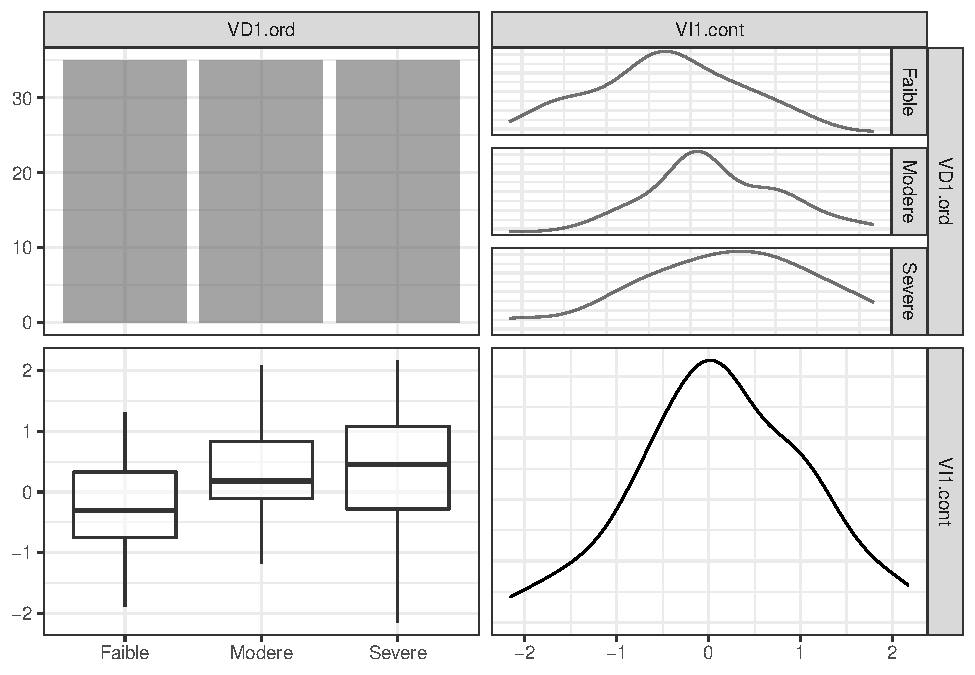
\includegraphics{Manuel_R_independant_files/figure-latex/unnamed-chunk-156-1.pdf}

\hypertarget{analyse-des-donnuxe9es-18}{%
\subsubsection{Analyse des données}\label{analyse-des-donnuxe9es-18}}

\begin{Shaded}
\begin{Highlighting}[]
\CommentTok{# Pour vérifier que vos catégories de VD1.ord ont bien été hierarchisées correctement}
\KeywordTok{str}\NormalTok{(my_data.regord2}\OperatorTok{$}\NormalTok{VD1.ord)}
\end{Highlighting}
\end{Shaded}

\begin{verbatim}
##  Ord.factor w/ 3 levels "Faible"<"Modere"<..: 1 1 1 1 1 1 1 1 1 1 ...
\end{verbatim}

\begin{Shaded}
\begin{Highlighting}[]
\CommentTok{# calcul du test de régression ordinale et stockage des résultats dans l’objet regord2.test}
\NormalTok{regord2.test <-}\StringTok{ }\NormalTok{MASS}\OperatorTok{::}\KeywordTok{polr}\NormalTok{(}\DataTypeTok{formula =} \KeywordTok{ordered}\NormalTok{(VD1.ord) }\OperatorTok{~}\StringTok{ }\NormalTok{VI1.cont, }
                           \DataTypeTok{data =}\NormalTok{ my_data.regord2)}

\CommentTok{# calcul des odds ratio}
\NormalTok{oddsratio.regord2 <-}\StringTok{ }\KeywordTok{exp}\NormalTok{(}\KeywordTok{coef}\NormalTok{(}\KeywordTok{summary}\NormalTok{(regord2.test)))}

\CommentTok{# obtention des résultats de la régression logistique ordinale}
\KeywordTok{Anova}\NormalTok{(regord2.test)}
\end{Highlighting}
\end{Shaded}

\begin{verbatim}
## Analysis of Deviance Table (Type II tests)
## 
## Response: ordered(VD1.ord)
##          LR Chisq Df Pr(>Chisq)   
## VI1.cont   8.9571  1   0.002764 **
## ---
## Signif. codes:  0 '***' 0.001 '**' 0.01 '*' 0.05 '.' 0.1 ' ' 1
\end{verbatim}

\begin{Shaded}
\begin{Highlighting}[]
\CommentTok{# obtention de la taille d'effet}
\NormalTok{oddsratio.regord2}
\end{Highlighting}
\end{Shaded}

\begin{verbatim}
##                   Value Std. Error     t value
## VI1.cont      1.8565100   1.237809 18.17457892
## Faible|Modere 0.5343113   1.237832  0.05299107
## Modere|Severe 2.3600219   1.249030 47.53678752
\end{verbatim}

\hypertarget{graphique-18}{%
\subsubsection{Graphique}\label{graphique-18}}

\begin{Shaded}
\begin{Highlighting}[]
\NormalTok{crude.slope.regord2 <-}\StringTok{ }\KeywordTok{as.data.frame}\NormalTok{(}
  \KeywordTok{effect}\NormalTok{(}
    \DataTypeTok{term=}\StringTok{"VI1.cont"}\NormalTok{, }
    \DataTypeTok{mod =}\NormalTok{ regord2.test))}

\NormalTok{crude.slope.regord2.long <-}\StringTok{ }\NormalTok{crude.slope.regord2 }\OperatorTok\StringTok{ }
\StringTok{    }\NormalTok{dplyr}\OperatorTok{::}\KeywordTok{select}\NormalTok{(VI1.cont, }
\NormalTok{                  prob.Faible,}
\NormalTok{                  prob.Modere,}
\NormalTok{                  prob.Severe) }\OperatorTok
\StringTok{    }\KeywordTok{pivot_longer}\NormalTok{(}\OperatorTok{-}\NormalTok{VI1.cont, }
        \DataTypeTok{names_to=}\StringTok{"VD1.ord"}\NormalTok{,}
        \DataTypeTok{values_to=}\StringTok{"VD"}\NormalTok{)}

\NormalTok{crude.slope.regord2.long}\OperatorTok{$}\NormalTok{VD1.ord<-}\StringTok{ }\KeywordTok{fct_recode}\NormalTok{(crude.slope.regord2.long}\OperatorTok{$}\NormalTok{VD1.ord,}
    \StringTok{"Faible"}\NormalTok{ =}\StringTok{ "prob.Faible"}\NormalTok{, }
    \StringTok{"Modere"}\NormalTok{ =}\StringTok{ "prob.Modere"}\NormalTok{,}
    \StringTok{"Severe"}\NormalTok{ =}\StringTok{ "prob.Severe"}\NormalTok{)}

\NormalTok{crude.slope.regord2.long}\OperatorTok{$}\NormalTok{VD1.ord <-}\StringTok{ }\KeywordTok{ordered}\NormalTok{(crude.slope.regord2.long}\OperatorTok{$}\NormalTok{VD1.ord, }
        \DataTypeTok{levels =} \KeywordTok{c}\NormalTok{(}\StringTok{"Faible"}\NormalTok{, }\StringTok{"Modere"}\NormalTok{, }\StringTok{"Severe"}\NormalTok{))}

\KeywordTok{ggplot}\NormalTok{(crude.slope.regord2.long) }\OperatorTok{+}\StringTok{ }
\StringTok{  }\KeywordTok{geom_line}\NormalTok{(}\KeywordTok{aes}\NormalTok{(}\DataTypeTok{x =}\NormalTok{ VI1.cont, }\DataTypeTok{y =}\NormalTok{ VD, }\DataTypeTok{color =}\NormalTok{ VD1.ord),  }\DataTypeTok{size =} \DecValTok{1}\NormalTok{) }\OperatorTok{+}\StringTok{ }
\StringTok{  }\KeywordTok{ylab}\NormalTok{(}\StringTok{"Probabilité"}\NormalTok{) }\OperatorTok{+}\StringTok{ }\KeywordTok{xlab}\NormalTok{(}\StringTok{"VI1.cont"}\NormalTok{) }\OperatorTok{+}
\StringTok{  }\KeywordTok{theme_bw}\NormalTok{() }\OperatorTok{+}\StringTok{ }
\StringTok{  }\KeywordTok{theme}\NormalTok{(}
    \DataTypeTok{axis.title.y =} \KeywordTok{element_text}\NormalTok{(}\DataTypeTok{size =} \DecValTok{14}\NormalTok{, }\DataTypeTok{hjust =} \FloatTok{0.5}\NormalTok{, }\DataTypeTok{face =}\StringTok{"bold"}\NormalTok{), }
    \DataTypeTok{axis.title.x =} \KeywordTok{element_text}\NormalTok{(}\DataTypeTok{face =}\StringTok{"bold"}\NormalTok{, }\DataTypeTok{size =} \DecValTok{14}\NormalTok{, }\DataTypeTok{hjust =} \FloatTok{0.5}\NormalTok{)) }\OperatorTok{+}
\StringTok{  }\KeywordTok{scale_color_grey}\NormalTok{(}\DataTypeTok{start=}\FloatTok{0.9}\NormalTok{, }\DataTypeTok{end=}\FloatTok{0.1}\NormalTok{) }\OperatorTok{+}\StringTok{ }
\StringTok{  }\KeywordTok{scale_y_continuous}\NormalTok{(}\DataTypeTok{limits=}\KeywordTok{c}\NormalTok{(}\DecValTok{0}\NormalTok{,}\DecValTok{1}\NormalTok{))}
\end{Highlighting}
\end{Shaded}

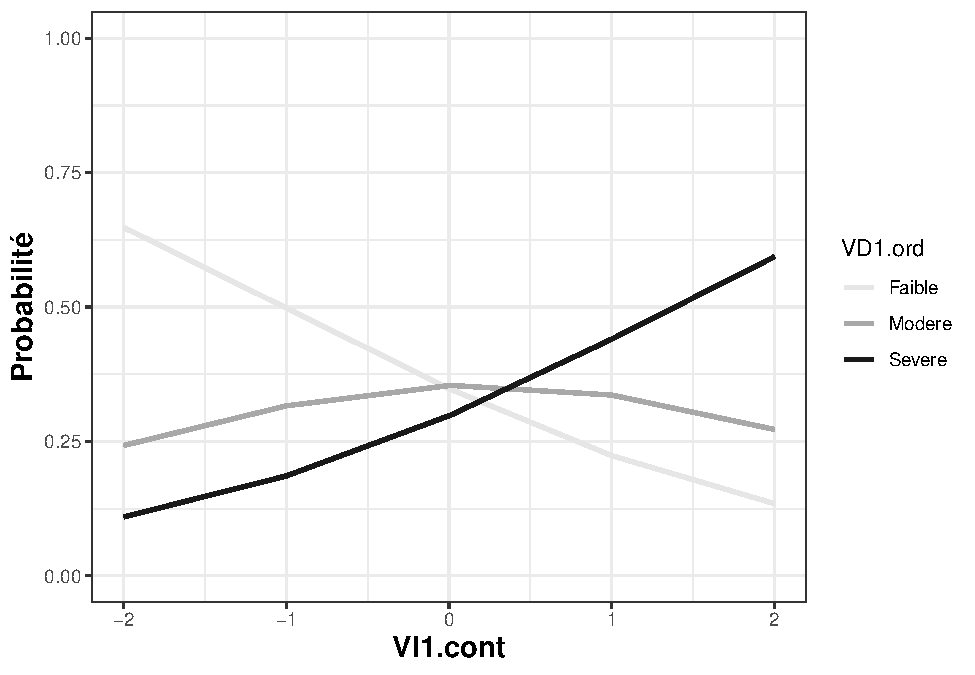
\includegraphics{Manuel_R_independant_files/figure-latex/unnamed-chunk-158-1.pdf}

\hypertarget{interpretation-18}{%
\subsubsection{Interpretation}\label{interpretation-18}}

{[}1{]} ``La probabilité d'obtenir un score sévère à VD1.ord (comparativement à un score faible ou modéré) augmente à mesure que VI1.cont augmente (X² = 8.957, OR = 1.857, p = 0.0028).''

\hypertarget{ruxe9gression-logistique-ordinale-3}{%
\subsection{Régression logistique ordinale 3}\label{ruxe9gression-logistique-ordinale-3}}

\hypertarget{type-de-variables-19}{%
\subsubsection{Type de variables}\label{type-de-variables-19}}

\textbf{Variable Dépendante :} Ordinale (3 catégories ou +)
\textbf{Variables Indépendantes :} Numériques / Catégorielles (2 catégories ou +)

\hypertarget{packages-nuxe9cessaires-19}{%
\subsubsection{Packages nécessaires}\label{packages-nuxe9cessaires-19}}

\begin{Shaded}
\begin{Highlighting}[]
\KeywordTok{library}\NormalTok{(ggplot2)}
\KeywordTok{library}\NormalTok{(GGally)}
\KeywordTok{library}\NormalTok{(forcats)}
\KeywordTok{library}\NormalTok{(dplyr)}
\KeywordTok{library}\NormalTok{(car)}
\KeywordTok{library}\NormalTok{(effects)}
\KeywordTok{library}\NormalTok{(tidyr)}
\KeywordTok{library}\NormalTok{(broom)}
\end{Highlighting}
\end{Shaded}

\hypertarget{donnuxe9es-ruxe9elles-19}{%
\subsubsection{Données réelles}\label{donnuxe9es-ruxe9elles-19}}

\begin{Shaded}
\begin{Highlighting}[]
\CommentTok{# choisissez la ligne appropriée au format de votre fichier de données. }

\CommentTok{# si vos données sont dans un fichier .txt}
\NormalTok{my_data.regord3 <-}\StringTok{ }\KeywordTok{read.delim}\NormalTok{(}\KeywordTok{file.choose}\NormalTok{())}

\CommentTok{# si vos données sont dans un fichier .csv}
\NormalTok{my_data.regord3 <-}\StringTok{ }\KeywordTok{read.csv}\NormalTok{(}\KeywordTok{file.choose}\NormalTok{())}

\CommentTok{# si vos données sont dans un fichier .xls / .xlsx}
\NormalTok{my_data.regord3 <-}\StringTok{ }\KeywordTok{read_excel}\NormalTok{(}\KeywordTok{file.choose}\NormalTok{())}

\CommentTok{# une fois vos données chargées, vous pouvez renommer vos noms de colonnes afin qu'ils correspondent à ceux utilisés dans le code ci-dessous}
\CommentTok{# Si vous ne souhaitez pas renommer vos noms de colonnes, sautez cette étape mais adaptez le code des parties suivantes en lui indiquant les noms de colonnes de vos données.}

\CommentTok{# On crée une nouvelle colonne pour votre variable dépendante ordinale (remplacez 'votre.nom.de.colonne' par le nom approprié)}
\NormalTok{my_data.regord3}\OperatorTok{$}\NormalTok{VD1.ord <-}\StringTok{ }\NormalTok{my_data.regord3}\OperatorTok{$}\StringTok{'votre.nom.de.colonne'}

\CommentTok{# On crée une nouvelle colonne pour vos variables indépendantes catégorielles (remplacez 'votre.nom.de.colonne' par les noms appropriés)}
\NormalTok{my_data.regord3}\OperatorTok{$}\NormalTok{VI1.cat <-}\StringTok{ }\NormalTok{my_data.regord3}\OperatorTok{$}\StringTok{'votre.nom.de.colonne'}
\NormalTok{my_data.regord3}\OperatorTok{$}\NormalTok{VI2.multicat <-}\StringTok{ }\NormalTok{my_data.regord3}\OperatorTok{$}\StringTok{'votre.nom.de.colonne'}

\CommentTok{# On crée une nouvelle colonne pour votre variable indépendante continue (remplacez 'votre.nom.de.colonne' par le nom approprié)}
\NormalTok{my_data.regord3}\OperatorTok{$}\NormalTok{VI1.cont <-}\StringTok{ }\NormalTok{my_data.regord3}\OperatorTok{$}\StringTok{'votre.nom.de.colonne'}
\end{Highlighting}
\end{Shaded}

\hypertarget{donnuxe9es-fictives-19}{%
\subsubsection{Données fictives}\label{donnuxe9es-fictives-19}}

\begin{Shaded}
\begin{Highlighting}[]
\KeywordTok{set.seed}\NormalTok{(}\DecValTok{4321}\NormalTok{)}
\NormalTok{regord3 <-}\StringTok{ }\KeywordTok{rbinom}\NormalTok{(}\DecValTok{200}\NormalTok{, }\DecValTok{1}\NormalTok{, }\FloatTok{0.8}\NormalTok{)}
\NormalTok{my_data.regord3 <-}\StringTok{ }\KeywordTok{data.frame}\NormalTok{(}
  \DataTypeTok{VD1.ord =}\NormalTok{ (}\KeywordTok{rbinom}\NormalTok{(}\DecValTok{200}\NormalTok{, }\DecValTok{2}\NormalTok{, }\FloatTok{0.5}\NormalTok{)}\OperatorTok{*}\NormalTok{regord3 }\OperatorTok{+}\StringTok{ }\DecValTok{1}\NormalTok{),}
  \DataTypeTok{VI1.cat =}\NormalTok{ (}\KeywordTok{rbinom}\NormalTok{(}\DecValTok{200}\NormalTok{, }\DecValTok{1}\NormalTok{, }\FloatTok{0.6}\NormalTok{)}\OperatorTok{*}\NormalTok{regord3 }\OperatorTok{+}\StringTok{ }\DecValTok{1}\NormalTok{),}
  \DataTypeTok{VI2.multicat =}\NormalTok{ (}\KeywordTok{rbinom}\NormalTok{(}\DecValTok{200}\NormalTok{, }\DecValTok{3}\NormalTok{, }\FloatTok{0.5}\NormalTok{)}\OperatorTok{*}\NormalTok{regord3),}
  \DataTypeTok{VI3.cont =} \KeywordTok{rnorm}\NormalTok{(}\DecValTok{200}\NormalTok{))}

\CommentTok{# on recode les catégories de VD1.ord, VI1.cat et VI2.multicat pour que les résultats soient plus lisibles}
\NormalTok{my_data.regord3}\OperatorTok{$}\NormalTok{VD1.ord <-}\StringTok{ }\KeywordTok{fct_recode}\NormalTok{(}\KeywordTok{factor}\NormalTok{(my_data.regord3}\OperatorTok{$}\NormalTok{VD1.ord), }
                                    \StringTok{"Faible"}\NormalTok{ =}\StringTok{ "1"}\NormalTok{, }
                                    \StringTok{"Modere"}\NormalTok{ =}\StringTok{ "2"}\NormalTok{,}
                                    \StringTok{"Severe"}\NormalTok{ =}\StringTok{ "3"}\NormalTok{) }

\NormalTok{my_data.regord3}\OperatorTok{$}\NormalTok{VI1.cat <-}\StringTok{ }\KeywordTok{fct_recode}\NormalTok{(}\KeywordTok{factor}\NormalTok{(my_data.regord3}\OperatorTok{$}\NormalTok{VI1.cat), }
                                    \StringTok{"Groupe 1"}\NormalTok{ =}\StringTok{ "1"}\NormalTok{, }
                                    \StringTok{"Groupe 2"}\NormalTok{ =}\StringTok{ "2"}\NormalTok{) }

\NormalTok{my_data.regord3}\OperatorTok{$}\NormalTok{VI2.multicat <-}\StringTok{ }\KeywordTok{fct_recode}\NormalTok{(}\KeywordTok{factor}\NormalTok{(my_data.regord3}\OperatorTok{$}\NormalTok{VI2.multicat), }
                                    \StringTok{"Caracteristique 1"}\NormalTok{ =}\StringTok{ "0"}\NormalTok{, }
                                    \StringTok{"Caracteristique 2"}\NormalTok{ =}\StringTok{ "1"}\NormalTok{,}
                                    \StringTok{"Caracteristique 3"}\NormalTok{ =}\StringTok{ "2"}\NormalTok{,}
                                    \StringTok{"Caracteristique 4"}\NormalTok{ =}\StringTok{ "3"}\NormalTok{) }
\end{Highlighting}
\end{Shaded}

\hypertarget{duxe9claration-du-type-de-variables-18}{%
\subsubsection{Déclaration du type de variables}\label{duxe9claration-du-type-de-variables-18}}

\begin{Shaded}
\begin{Highlighting}[]
\NormalTok{my_data.regord3}\OperatorTok{$}\NormalTok{VD1.ord <-}\StringTok{ }\KeywordTok{ordered}\NormalTok{(my_data.regord3}\OperatorTok{$}\NormalTok{VD1.ord, }
                                   \DataTypeTok{levels =} \KeywordTok{c}\NormalTok{(}\StringTok{"Faible"}\NormalTok{, }\StringTok{"Modere"}\NormalTok{, }\StringTok{"Severe"}\NormalTok{))}
\NormalTok{my_data.regord3}\OperatorTok{$}\NormalTok{VI1.cat <-}\StringTok{ }\KeywordTok{factor}\NormalTok{(my_data.regord3}\OperatorTok{$}\NormalTok{VI1.cat)}
\NormalTok{my_data.regord3}\OperatorTok{$}\NormalTok{VI2.multicat <-}\StringTok{ }\KeywordTok{factor}\NormalTok{(my_data.regord3}\OperatorTok{$}\NormalTok{VI2.multicat)}
\NormalTok{my_data.regord3}\OperatorTok{$}\NormalTok{VI3.cont <-}\KeywordTok{as.numeric}\NormalTok{(}\KeywordTok{as.character}\NormalTok{(my_data.regord3}\OperatorTok{$}\NormalTok{VI3.cont))}
\end{Highlighting}
\end{Shaded}

\hypertarget{inspection-des-donnuxe9es-18}{%
\subsubsection{Inspection des données}\label{inspection-des-donnuxe9es-18}}

\begin{Shaded}
\begin{Highlighting}[]
\CommentTok{## Les graphiques situés sur la diagonale représentent la distribution des variables}
\CommentTok{## Les graphiques (ou les valeurs de corrélation) situés au dessus et en dessous de la diagonale représentent l'association entre les différentes variables}
\KeywordTok{ggpairs}\NormalTok{(my_data.regord3,}
        \DataTypeTok{lower =} \KeywordTok{list}\NormalTok{(}\DataTypeTok{continuous =} \KeywordTok{wrap}\NormalTok{(}\StringTok{"smooth"}\NormalTok{, }\DataTypeTok{alpha =} \FloatTok{0.7}\NormalTok{), }\DataTypeTok{combo =} \StringTok{"box_no_facet"}\NormalTok{),}
        \DataTypeTok{upper =} \KeywordTok{list}\NormalTok{(}\DataTypeTok{combo =} \StringTok{"facetdensity"}\NormalTok{, }\DataTypeTok{discrete =} \StringTok{"facetbar"}\NormalTok{), }
        \DataTypeTok{mapping =} \KeywordTok{aes}\NormalTok{(}\DataTypeTok{alpha =} \FloatTok{0.8}\NormalTok{)) }\OperatorTok{+}\StringTok{ }\KeywordTok{theme_bw}\NormalTok{()}
\end{Highlighting}
\end{Shaded}

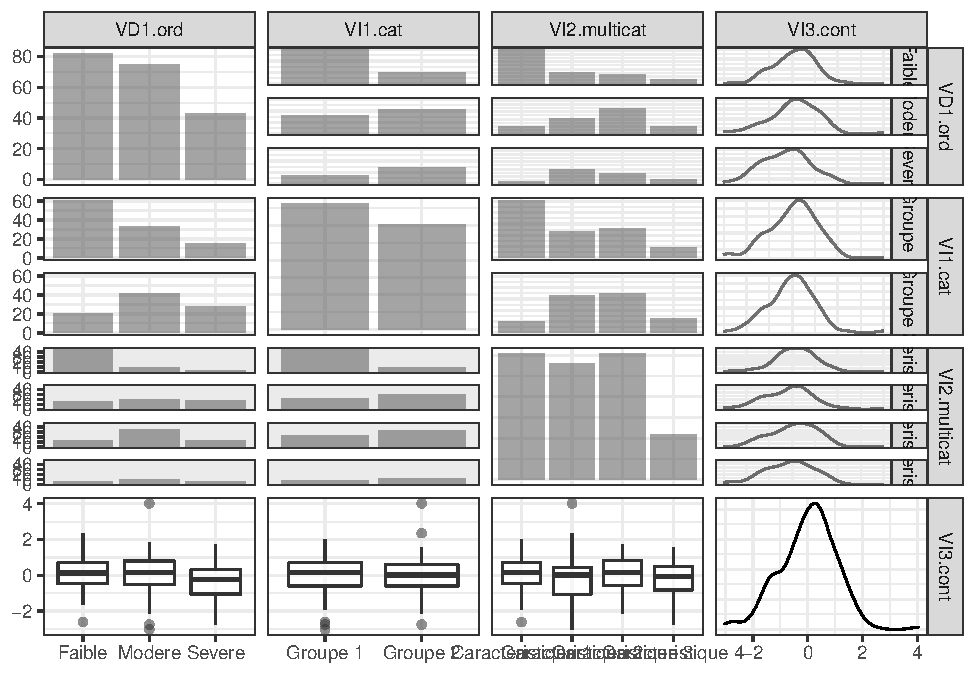
\includegraphics{Manuel_R_independant_files/figure-latex/unnamed-chunk-164-1.pdf}

\hypertarget{analyse-des-donnuxe9es-19}{%
\subsubsection{Analyse des données}\label{analyse-des-donnuxe9es-19}}

\begin{Shaded}
\begin{Highlighting}[]
\CommentTok{# pour vérifier que vos catégories de VD1.ord ont bien été hierarchisées correctement}
\KeywordTok{str}\NormalTok{(my_data.regord3}\OperatorTok{$}\NormalTok{VD1.ord)}
\end{Highlighting}
\end{Shaded}

\begin{verbatim}
##  Ord.factor w/ 3 levels "Faible"<"Modere"<..: 3 1 2 2 1 2 2 1 3 2 ...
\end{verbatim}

\begin{Shaded}
\begin{Highlighting}[]
\CommentTok{# calcul du test de régression ordinale et stockage des résultats dans l’objet regord3.test}
\NormalTok{regord3.test <-}\StringTok{ }\NormalTok{MASS}\OperatorTok{::}\KeywordTok{polr}\NormalTok{(}\DataTypeTok{formula =}\NormalTok{ VD1.ord }\OperatorTok{~}\StringTok{ }\NormalTok{VI1.cat }\OperatorTok{+}\StringTok{ }\NormalTok{VI2.multicat }\OperatorTok{+}\StringTok{ }\NormalTok{VI3.cont, }
                           \DataTypeTok{data =}\NormalTok{ my_data.regord3)}

\CommentTok{# calcul de la taille d'effet de VI1.cat sur VD1.ord (odds ratio ajusté par l'effet de VI2.multicat)}
\NormalTok{oddsratio.regord3 <-}\StringTok{ }\KeywordTok{exp}\NormalTok{(}\KeywordTok{coef}\NormalTok{(}\KeywordTok{summary}\NormalTok{(regord3.test)))}

\CommentTok{# obtention des résultats de la régression logistique ordinale}
\KeywordTok{Anova}\NormalTok{(regord3.test)}
\end{Highlighting}
\end{Shaded}

\begin{verbatim}
## Analysis of Deviance Table (Type II tests)
## 
## Response: VD1.ord
##              LR Chisq Df Pr(>Chisq)    
## VI1.cat        7.3574  1   0.006679 ** 
## VI2.multicat  31.3003  3  7.349e-07 ***
## VI3.cont       1.8682  1   0.171680    
## ---
## Signif. codes:  0 '***' 0.001 '**' 0.01 '*' 0.05 '.' 0.1 ' ' 1
\end{verbatim}

\begin{Shaded}
\begin{Highlighting}[]
\CommentTok{# obtention de la taille d'effet}
\NormalTok{oddsratio.regord3}
\end{Highlighting}
\end{Shaded}

\begin{verbatim}
##                                   Value Std. Error      t value
## VI1.catGroupe 2                2.242658   1.348506   14.8980760
## VI2.multicatCaracteristique 2  7.341798   1.525543  112.1918529
## VI2.multicatCaracteristique 3  6.756080   1.501548  109.9224311
## VI2.multicatCaracteristique 4  6.053035   1.681173   32.0084911
## VI3.cont                       0.833781   1.142465    0.2554152
## Faible|Modere                  3.698366   1.367037   65.5821571
## Modere|Severe                 28.004948   1.452782 7498.8958611
\end{verbatim}

\hypertarget{graphique-19}{%
\subsubsection{Graphique}\label{graphique-19}}

\begin{Shaded}
\begin{Highlighting}[]
\NormalTok{adjusted.slope.regord3 <-}\StringTok{ }\KeywordTok{as.data.frame}\NormalTok{(}
  \KeywordTok{effect}\NormalTok{(}
    \DataTypeTok{term=}\StringTok{"VI1.cat"}\NormalTok{, }
    \DataTypeTok{mod =}\NormalTok{ regord3.test))}
\end{Highlighting}
\end{Shaded}

\begin{verbatim}
## 
## Re-fitting to get Hessian
\end{verbatim}

\begin{Shaded}
\begin{Highlighting}[]
\NormalTok{adjusted.slope.regord3.long.prob <-}\StringTok{ }\NormalTok{adjusted.slope.regord3 }\OperatorTok\StringTok{ }
\StringTok{    }\NormalTok{dplyr}\OperatorTok{::}\KeywordTok{select}\NormalTok{(VI1.cat, }
\NormalTok{                  prob.Faible,}
\NormalTok{                  prob.Modere,}
\NormalTok{                  prob.Severe) }\OperatorTok
\StringTok{    }\KeywordTok{pivot_longer}\NormalTok{(}\OperatorTok{-}\NormalTok{VI1.cat, }
        \DataTypeTok{names_to=}\StringTok{"VD1.ord"}\NormalTok{,}
        \DataTypeTok{values_to=}\StringTok{"VD"}\NormalTok{)}

\NormalTok{adjusted.slope.regord3.long.se <-}\StringTok{ }\NormalTok{adjusted.slope.regord3 }\OperatorTok\StringTok{ }
\StringTok{    }\NormalTok{dplyr}\OperatorTok{::}\KeywordTok{select}\NormalTok{(VI1.cat, }
\NormalTok{                  se.prob.Faible,}
\NormalTok{                  se.prob.Modere,}
\NormalTok{                  se.prob.Severe) }\OperatorTok
\StringTok{    }\KeywordTok{pivot_longer}\NormalTok{(}\OperatorTok{-}\NormalTok{VI1.cat, }
        \DataTypeTok{names_to=}\StringTok{"VD1.ord.se"}\NormalTok{,}
        \DataTypeTok{values_to=}\StringTok{"SE"}\NormalTok{)}

\NormalTok{adjusted.slope.regord3.long <-}\StringTok{ }\KeywordTok{cbind}\NormalTok{(adjusted.slope.regord3.long.prob,                                    adjusted.slope.regord3.long.se[,}\KeywordTok{c}\NormalTok{(}\StringTok{'VD1.ord.se'}\NormalTok{, }\StringTok{'SE'}\NormalTok{)])}

\NormalTok{adjusted.slope.regord3.long}\OperatorTok{$}\NormalTok{VD1.ord<-}\StringTok{ }\KeywordTok{fct_recode}\NormalTok{(adjusted.slope.regord3.long}\OperatorTok{$}\NormalTok{VD1.ord,}
    \StringTok{"Faible"}\NormalTok{ =}\StringTok{ "prob.Faible"}\NormalTok{, }
    \StringTok{"Modere"}\NormalTok{ =}\StringTok{ "prob.Modere"}\NormalTok{,}
    \StringTok{"Severe"}\NormalTok{ =}\StringTok{ "prob.Severe"}\NormalTok{)}

\NormalTok{adjusted.slope.regord3.long}\OperatorTok{$}\NormalTok{VD1.ord <-}\StringTok{ }\KeywordTok{factor}\NormalTok{(adjusted.slope.regord3.long}\OperatorTok{$}\NormalTok{VD1.ord, }
        \DataTypeTok{levels =} \KeywordTok{c}\NormalTok{(}\StringTok{"Faible"}\NormalTok{, }\StringTok{"Modere"}\NormalTok{, }\StringTok{"Severe"}\NormalTok{))}

\KeywordTok{ggplot}\NormalTok{(adjusted.slope.regord3.long, }
       \KeywordTok{aes}\NormalTok{(}\DataTypeTok{x =}\NormalTok{ VI1.cat, }\DataTypeTok{y =}\NormalTok{ VD, }\DataTypeTok{color =}\NormalTok{ VD1.ord)) }\OperatorTok{+}\StringTok{ }
\StringTok{  }\KeywordTok{geom_errorbar}\NormalTok{(}\KeywordTok{aes}\NormalTok{(}
      \DataTypeTok{ymin =}\NormalTok{ VD }\OperatorTok{-}\StringTok{ }\NormalTok{SE,}
      \DataTypeTok{ymax =}\NormalTok{ VD }\OperatorTok{+}\StringTok{ }\NormalTok{SE),}
      \DataTypeTok{width =} \DecValTok{0}\NormalTok{, }\DataTypeTok{position =} \KeywordTok{position_dodge}\NormalTok{(}\FloatTok{0.3}\NormalTok{)) }\OperatorTok{+}
\StringTok{  }\KeywordTok{geom_point}\NormalTok{(}\DataTypeTok{size =} \DecValTok{2}\NormalTok{, }\DataTypeTok{position =} \KeywordTok{position_dodge}\NormalTok{(}\FloatTok{0.3}\NormalTok{)) }\OperatorTok{+}
\StringTok{  }\KeywordTok{ylab}\NormalTok{(}\StringTok{"Probabilité"}\NormalTok{) }\OperatorTok{+}\StringTok{ }\KeywordTok{xlab}\NormalTok{(}\StringTok{"VI1.cat"}\NormalTok{) }\OperatorTok{+}
\StringTok{  }\KeywordTok{theme_bw}\NormalTok{() }\OperatorTok{+}\StringTok{ }
\StringTok{  }\KeywordTok{theme}\NormalTok{(}
    \DataTypeTok{axis.title.y =} \KeywordTok{element_text}\NormalTok{(}\DataTypeTok{size =} \DecValTok{14}\NormalTok{, }\DataTypeTok{hjust =} \FloatTok{0.5}\NormalTok{, }\DataTypeTok{face =}\StringTok{"bold"}\NormalTok{), }
    \DataTypeTok{axis.title.x =} \KeywordTok{element_text}\NormalTok{(}\DataTypeTok{face =}\StringTok{"bold"}\NormalTok{, }\DataTypeTok{size =} \DecValTok{14}\NormalTok{, }\DataTypeTok{hjust =} \FloatTok{0.5}\NormalTok{)) }\OperatorTok{+}
\StringTok{  }\KeywordTok{scale_color_grey}\NormalTok{(}\DataTypeTok{start=}\FloatTok{0.7}\NormalTok{, }\DataTypeTok{end=}\FloatTok{0.01}\NormalTok{) }\OperatorTok{+}\StringTok{ }
\StringTok{  }\KeywordTok{scale_y_continuous}\NormalTok{(}\DataTypeTok{limits=}\KeywordTok{c}\NormalTok{(}\DecValTok{0}\NormalTok{,}\DecValTok{1}\NormalTok{))}
\end{Highlighting}
\end{Shaded}

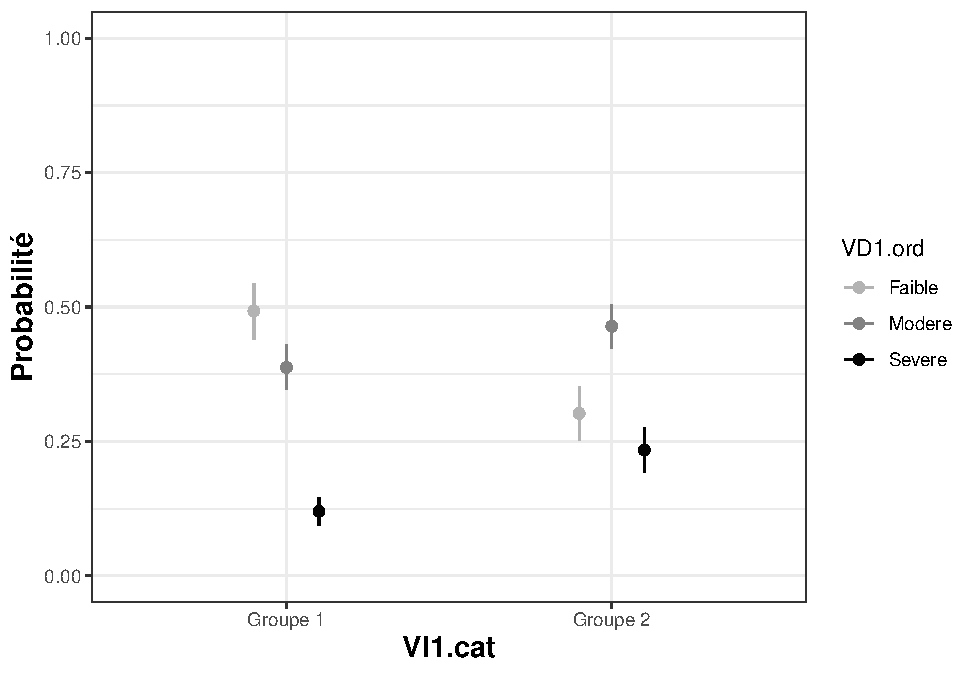
\includegraphics{Manuel_R_independant_files/figure-latex/unnamed-chunk-166-1.pdf}

\hypertarget{interpretation-19}{%
\subsubsection{Interpretation}\label{interpretation-19}}

{[}1{]} ``La probabilité d'obtenir un score faible à VD1.ord (comparativement à un score modéré ou sévère) est plus importante dans le groupe 1 que dans le groupe 2 même lorsque l'on ajuste par VI2.multicat (X² = 7.357, Odds ratio = 2.243, p = 0.0066788).''

\hypertarget{plusieurs-vd-numuxe9riques}{%
\section{Plusieurs VD numériques}\label{plusieurs-vd-numuxe9riques}}

\hypertarget{manova}{%
\subsection{MANOVA}\label{manova}}

\hypertarget{type-de-variables-20}{%
\subsubsection{Type de variables}\label{type-de-variables-20}}

\textbf{Variables Dépendantes :} Numérique
\textbf{Variables Indépendantes :} Catégorielles

\hypertarget{packages-nuxe9cessaires-20}{%
\subsubsection{Packages nécessaires}\label{packages-nuxe9cessaires-20}}

\begin{Shaded}
\begin{Highlighting}[]
\KeywordTok{library}\NormalTok{(ggplot2)}
\KeywordTok{library}\NormalTok{(GGally)}
\KeywordTok{library}\NormalTok{(rstatix)}
\KeywordTok{library}\NormalTok{(dplyr)}
\KeywordTok{library}\NormalTok{(effects)}
\KeywordTok{library}\NormalTok{(forcats)}
\KeywordTok{library}\NormalTok{(emmeans)}
\KeywordTok{library}\NormalTok{(tidyr)}
\end{Highlighting}
\end{Shaded}

\hypertarget{donnuxe9es-ruxe9elles-20}{%
\subsubsection{Données réelles}\label{donnuxe9es-ruxe9elles-20}}

\begin{Shaded}
\begin{Highlighting}[]
\CommentTok{# choisissez la ligne appropriée au format de votre fichier de données. }

\CommentTok{# si vos données sont dans un fichier .txt}
\NormalTok{my_data.manova <-}\StringTok{ }\KeywordTok{read.delim}\NormalTok{(}\KeywordTok{file.choose}\NormalTok{())}

\CommentTok{# si vos données sont dans un fichier .csv}
\NormalTok{my_data.manova <-}\StringTok{ }\KeywordTok{read.csv}\NormalTok{(}\KeywordTok{file.choose}\NormalTok{())}

\CommentTok{# si vos données sont dans un fichier .xls / .xlsx}
\NormalTok{my_data.manova <-}\StringTok{ }\KeywordTok{read_excel}\NormalTok{(}\KeywordTok{file.choose}\NormalTok{())}

\CommentTok{# une fois vos données chargées, vous pouvez renommer vos noms de colonnes afin qu'ils correspondent à ceux utilisés dans le code ci-dessous}
\CommentTok{# Si vous ne souhaitez pas renommer vos noms de colonnes, sautez cette étape mais adaptez le code des parties suivantes en lui indiquant les noms de colonnes de vos données.}

\CommentTok{# On crée une nouvelle colonne pour vos variables dépendantes continues (remplacez 'votre.nom.de.colonne' par les noms appropriés)}
\NormalTok{my_data.manova}\OperatorTok{$}\NormalTok{VD1.cont <-}\StringTok{ }\NormalTok{my_data.manova}\OperatorTok{$}\StringTok{'votre.nom.de.colonne'}
\NormalTok{my_data.manova}\OperatorTok{$}\NormalTok{VD2.cont <-}\StringTok{ }\NormalTok{my_data.manova}\OperatorTok{$}\StringTok{'votre.nom.de.colonne'}

\CommentTok{# On crée une nouvelle colonne pour vos variables indépendantes catégorielles (remplacez 'votre.nom.de.colonne' par les noms appropriés)}
\NormalTok{my_data.manova}\OperatorTok{$}\NormalTok{VI1.cat <-}\StringTok{ }\NormalTok{my_data.manova}\OperatorTok{$}\StringTok{'votre.nom.de.colonne'}
\NormalTok{my_data.manova}\OperatorTok{$}\NormalTok{VI2.cat <-}\StringTok{ }\NormalTok{my_data.manova}\OperatorTok{$}\StringTok{'votre.nom.de.colonne'}
\end{Highlighting}
\end{Shaded}

\hypertarget{donnuxe9es-fictives-20}{%
\subsubsection{Données fictives}\label{donnuxe9es-fictives-20}}

\begin{Shaded}
\begin{Highlighting}[]
\KeywordTok{set.seed}\NormalTok{(}\DecValTok{4321}\NormalTok{)}
\NormalTok{manova <-}\StringTok{ }\KeywordTok{rnorm}\NormalTok{(}\DecValTok{50}\NormalTok{)}
\NormalTok{my_data.manova <-}\StringTok{ }\KeywordTok{data.frame}\NormalTok{(}
  \DataTypeTok{VD1.cont =} \KeywordTok{rnorm}\NormalTok{(}\DecValTok{50}\NormalTok{)}\OperatorTok{*}\DecValTok{2} \OperatorTok{+}\StringTok{ }\DecValTok{1}\OperatorTok{*}\NormalTok{manova,}
  \DataTypeTok{VD2.cont =} \KeywordTok{rnorm}\NormalTok{(}\DecValTok{50}\NormalTok{)}\OperatorTok{+}\StringTok{ }\FloatTok{0.2}\OperatorTok{*}\NormalTok{manova,}
  \DataTypeTok{VI1.cat =} \KeywordTok{rep}\NormalTok{(}\KeywordTok{c}\NormalTok{(}\DecValTok{1}\NormalTok{,}\DecValTok{2}\NormalTok{), }\DataTypeTok{each=}\DecValTok{25}\NormalTok{),}
  \DataTypeTok{VI2.cat =} \KeywordTok{rbinom}\NormalTok{(}\DecValTok{50}\NormalTok{, }\DecValTok{1}\NormalTok{, }\FloatTok{0.5}\NormalTok{) }\OperatorTok{+}\StringTok{ }\DecValTok{1}\NormalTok{)}

\CommentTok{# on recode les catégories de VI1.cat et VI2.cat pour que les résultats soient plus lisibles}
\NormalTok{my_data.manova}\OperatorTok{$}\NormalTok{VI1.cat <-}\StringTok{ }\KeywordTok{fct_recode}\NormalTok{(}\KeywordTok{factor}\NormalTok{(my_data.manova}\OperatorTok{$}\NormalTok{VI1.cat), }
                                    \StringTok{"Groupe 1"}\NormalTok{ =}\StringTok{ "1"}\NormalTok{, }
                                    \StringTok{"Groupe 2"}\NormalTok{ =}\StringTok{ "2"}\NormalTok{) }

\NormalTok{my_data.manova}\OperatorTok{$}\NormalTok{VI2.cat <-}\StringTok{ }\KeywordTok{fct_recode}\NormalTok{(}\KeywordTok{factor}\NormalTok{(my_data.manova}\OperatorTok{$}\NormalTok{VI2.cat), }
                                    \StringTok{"Caracteristique 1"}\NormalTok{ =}\StringTok{ "1"}\NormalTok{, }
                                    \StringTok{"Caracteristique 2"}\NormalTok{ =}\StringTok{ "2"}\NormalTok{) }
\end{Highlighting}
\end{Shaded}

\hypertarget{duxe9claration-du-type-de-variables-19}{%
\subsubsection{Déclaration du type de variables}\label{duxe9claration-du-type-de-variables-19}}

\begin{Shaded}
\begin{Highlighting}[]
\NormalTok{my_data.manova}\OperatorTok{$}\NormalTok{VD1.cont <-}\StringTok{ }\KeywordTok{as.numeric}\NormalTok{(}\KeywordTok{as.character}\NormalTok{(my_data.manova}\OperatorTok{$}\NormalTok{VD1.cont))}
\NormalTok{my_data.manova}\OperatorTok{$}\NormalTok{VD2.cont <-}\StringTok{ }\KeywordTok{as.numeric}\NormalTok{(}\KeywordTok{as.character}\NormalTok{(my_data.manova}\OperatorTok{$}\NormalTok{VD2.cont))}
\NormalTok{my_data.manova}\OperatorTok{$}\NormalTok{VI1.cat <-}\StringTok{ }\KeywordTok{factor}\NormalTok{(my_data.manova}\OperatorTok{$}\NormalTok{VI1.cat)}
\NormalTok{my_data.manova}\OperatorTok{$}\NormalTok{VI2.cat <-}\StringTok{ }\KeywordTok{factor}\NormalTok{(my_data.manova}\OperatorTok{$}\NormalTok{VI2.cat)}
\end{Highlighting}
\end{Shaded}

\hypertarget{inspection-des-donnuxe9es-19}{%
\subsubsection{Inspection des données}\label{inspection-des-donnuxe9es-19}}

\begin{Shaded}
\begin{Highlighting}[]
\CommentTok{## Les graphiques situés sur la diagonale représentent la distribution des variables}
\CommentTok{## Les graphiques (ou les valeurs de corrélation) situés au dessus et en dessous de la diagonale représentent l'association entre les différentes variables}
\KeywordTok{ggpairs}\NormalTok{(my_data.manova,}
        \DataTypeTok{lower =} \KeywordTok{list}\NormalTok{(}\DataTypeTok{continuous =} \KeywordTok{wrap}\NormalTok{(}\StringTok{"smooth"}\NormalTok{, }\DataTypeTok{alpha =} \FloatTok{0.7}\NormalTok{), }\DataTypeTok{combo =} \StringTok{"box_no_facet"}\NormalTok{),}
        \DataTypeTok{upper =} \KeywordTok{list}\NormalTok{(}\DataTypeTok{combo =} \StringTok{"facetdensity"}\NormalTok{, }\DataTypeTok{discrete =} \StringTok{"facetbar"}\NormalTok{), }
        \DataTypeTok{mapping =} \KeywordTok{aes}\NormalTok{(}\DataTypeTok{alpha =} \FloatTok{0.8}\NormalTok{)) }\OperatorTok{+}\StringTok{ }\KeywordTok{theme_bw}\NormalTok{()}
\end{Highlighting}
\end{Shaded}

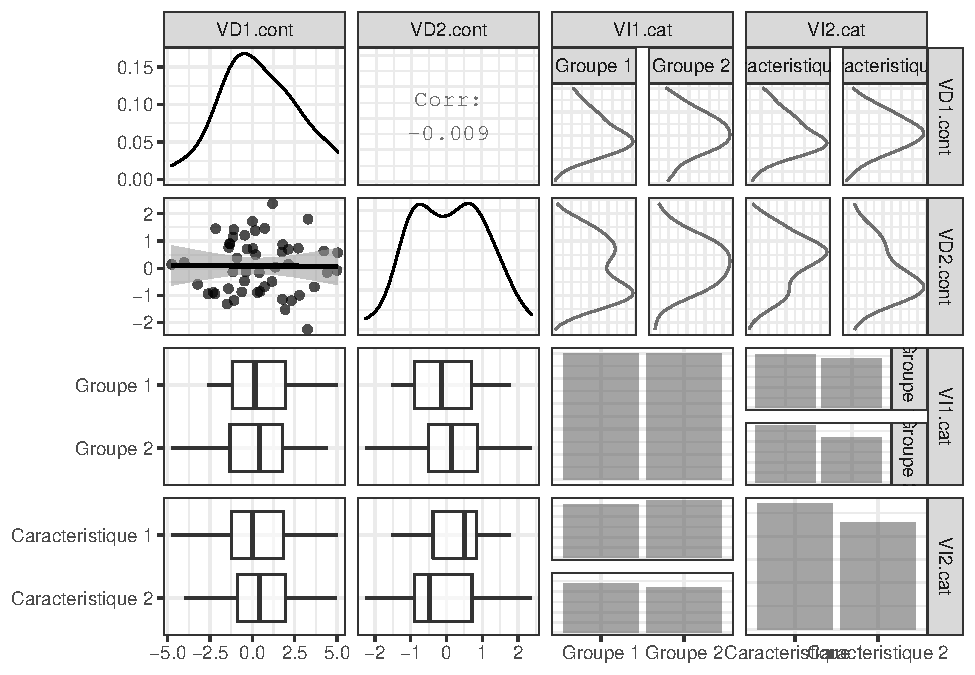
\includegraphics{Manuel_R_independant_files/figure-latex/unnamed-chunk-172-1.pdf}

\hypertarget{analyse-des-donnuxe9es-20}{%
\subsubsection{Analyse des données}\label{analyse-des-donnuxe9es-20}}

\begin{Shaded}
\begin{Highlighting}[]
\CommentTok{# calcul de la manova et stockage des résultats dans l’objet manova.test}
\NormalTok{manova.test <-}\StringTok{ }\KeywordTok{lm}\NormalTok{(}\DataTypeTok{formula =} \KeywordTok{cbind}\NormalTok{(VD1.cont, VD2.cont) }\OperatorTok{~}\StringTok{ }\NormalTok{VI1.cat}\OperatorTok{*}\NormalTok{VI2.cat, }
                  \DataTypeTok{contrasts =} \KeywordTok{list}\NormalTok{(}
                    \DataTypeTok{VI1.cat =} \StringTok{"contr.sum"}\NormalTok{,}
                    \DataTypeTok{VI2.cat =} \StringTok{"contr.sum"}\NormalTok{),}
                 \DataTypeTok{data =}\NormalTok{ my_data.manova)}

\CommentTok{# tests post-hocs évaluant l'effet principal de VI1.cat pour chaque modalité de VI2.cat et pour chaque variable dépendante (p-values non ajustées)}
\NormalTok{posthoc.manova <-}\StringTok{ }\KeywordTok{emmeans}\NormalTok{(manova.test, consec }\OperatorTok{~}\StringTok{ }\NormalTok{VI1.cat}\OperatorTok{|}\NormalTok{VD.mult}\OperatorTok{*}\NormalTok{VI2.cat, }\DataTypeTok{mult.names =} \StringTok{"VD.mult"}\NormalTok{)}

\CommentTok{# obtention des résultats de la manova}

\CommentTok{## résultats multivariés }
\KeywordTok{Anova}\NormalTok{(manova.test, }\DataTypeTok{type =} \DecValTok{3}\NormalTok{)}
\end{Highlighting}
\end{Shaded}

\begin{verbatim}
## 
## Type III MANOVA Tests: Pillai test statistic
##                 Df test stat approx F num Df den Df Pr(>F)
## (Intercept)      1  0.034148  0.79550      2     45 0.4576
## VI1.cat          1  0.012499  0.28480      2     45 0.7535
## VI2.cat          1  0.042506  0.99883      2     45 0.3763
## VI1.cat:VI2.cat  1  0.036214  0.84542      2     45 0.4361
\end{verbatim}

\begin{Shaded}
\begin{Highlighting}[]
\CommentTok{## résultats univariés }
\KeywordTok{summary}\NormalTok{(manova.test)}
\end{Highlighting}
\end{Shaded}

\begin{verbatim}
## Response VD1.cont :
## 
## Call:
## lm(formula = VD1.cont ~ VI1.cat * VI2.cat, data = my_data.manova, 
##     contrasts = list(VI1.cat = "contr.sum", VI2.cat = "contr.sum"))
## 
## Residuals:
##     Min      1Q  Median      3Q     Max 
## -4.6451 -1.2643 -0.1874  1.3982  4.6416 
## 
## Coefficients:
##                   Estimate Std. Error t value Pr(>|t|)
## (Intercept)        0.40036    0.32863   1.218    0.229
## VI1.cat1           0.15666    0.32863   0.477    0.636
## VI2.cat1          -0.08085    0.32863  -0.246    0.807
## VI1.cat1:VI2.cat1  0.27755    0.32863   0.845    0.403
## 
## Residual standard error: 2.314 on 46 degrees of freedom
## Multiple R-squared:  0.02295,	Adjusted R-squared:  -0.04077 
## F-statistic: 0.3602 on 3 and 46 DF,  p-value: 0.782
## 
## 
## Response VD2.cont :
## 
## Call:
## lm(formula = VD2.cont ~ VI1.cat * VI2.cat, data = my_data.manova, 
##     contrasts = list(VI1.cat = "contr.sum", VI2.cat = "contr.sum"))
## 
## Residuals:
##      Min       1Q   Median       3Q      Max 
## -2.05660 -0.77576 -0.08148  0.68083  2.57804 
## 
## Coefficients:
##                   Estimate Std. Error t value Pr(>|t|)
## (Intercept)        0.05850    0.14363   0.407    0.686
## VI1.cat1          -0.08385    0.14363  -0.584    0.562
## VI2.cat1           0.20125    0.14363   1.401    0.168
## VI1.cat1:VI2.cat1 -0.14165    0.14363  -0.986    0.329
## 
## Residual standard error: 1.012 on 46 degrees of freedom
## Multiple R-squared:  0.06956,	Adjusted R-squared:  0.008876 
## F-statistic: 1.146 on 3 and 46 DF,  p-value: 0.3405
\end{verbatim}

\begin{Shaded}
\begin{Highlighting}[]
\CommentTok{# résultats des tests post hoc}
\NormalTok{posthoc.manova}
\end{Highlighting}
\end{Shaded}

\begin{verbatim}
## $emmeans
## VD.mult = VD1.cont, VI2.cat = Caracteristique 1:
##  VI1.cat   emmean    SE df lower.CL upper.CL
##  Groupe 1  0.7537 0.642 46  -0.5384    2.046
##  Groupe 2 -0.1147 0.619 46  -1.3598    1.130
## 
## VD.mult = VD2.cont, VI2.cat = Caracteristique 1:
##  VI1.cat   emmean    SE df lower.CL upper.CL
##  Groupe 1  0.0342 0.281 46  -0.5305    0.599
##  Groupe 2  0.4852 0.270 46  -0.0589    1.029
## 
## VD.mult = VD1.cont, VI2.cat = Caracteristique 2:
##  VI1.cat   emmean    SE df lower.CL upper.CL
##  Groupe 1  0.3603 0.668 46  -0.9845    1.705
##  Groupe 2  0.6021 0.698 46  -0.8026    2.007
## 
## VD.mult = VD2.cont, VI2.cat = Caracteristique 2:
##  VI1.cat   emmean    SE df lower.CL upper.CL
##  Groupe 1 -0.0849 0.292 46  -0.6727    0.503
##  Groupe 2 -0.2006 0.305 46  -0.8145    0.413
## 
## Confidence level used: 0.95 
## 
## $contrasts
## VD.mult = VD1.cont, VI2.cat = Caracteristique 1:
##  contrast            estimate    SE df t.ratio p.value
##  Groupe 2 - Groupe 1   -0.868 0.891 46 -0.974  0.3351 
## 
## VD.mult = VD2.cont, VI2.cat = Caracteristique 1:
##  contrast            estimate    SE df t.ratio p.value
##  Groupe 2 - Groupe 1    0.451 0.390 46  1.158  0.2530 
## 
## VD.mult = VD1.cont, VI2.cat = Caracteristique 2:
##  contrast            estimate    SE df t.ratio p.value
##  Groupe 2 - Groupe 1    0.242 0.966 46  0.250  0.8035 
## 
## VD.mult = VD2.cont, VI2.cat = Caracteristique 2:
##  contrast            estimate    SE df t.ratio p.value
##  Groupe 2 - Groupe 1   -0.116 0.422 46 -0.274  0.7855
\end{verbatim}

\hypertarget{graphique-20}{%
\subsubsection{Graphique}\label{graphique-20}}

\begin{Shaded}
\begin{Highlighting}[]
\CommentTok{# graphique représentant les effets multivariés}
\NormalTok{crude.manova <-}\StringTok{ }\KeywordTok{do.call}\NormalTok{(rbind, }\KeywordTok{data.frame}\NormalTok{(}\KeywordTok{effect}\NormalTok{(}\DataTypeTok{term=}\StringTok{"VI1.cat*VI2.cat"}\NormalTok{, }\DataTypeTok{mod=}\NormalTok{ manova.test)))}
\NormalTok{crude.manova}\OperatorTok{$}\NormalTok{Outcome <-}\StringTok{ }\KeywordTok{rep}\NormalTok{(}\KeywordTok{c}\NormalTok{(}\StringTok{"VD1.cont"}\NormalTok{, }\StringTok{"VD2.cont"}\NormalTok{), }\DataTypeTok{each =} \KeywordTok{nrow}\NormalTok{(crude.manova)}\OperatorTok{/}\DecValTok{2}\NormalTok{)}

\KeywordTok{ggplot}\NormalTok{(crude.manova, }
       \KeywordTok{aes}\NormalTok{(}\DataTypeTok{x =}\NormalTok{ VI1.cat, }\DataTypeTok{y =}\NormalTok{ fit, }\DataTypeTok{fill =}\NormalTok{ VI1.cat)) }\OperatorTok{+}
\StringTok{  }\KeywordTok{geom_hline}\NormalTok{(}\KeywordTok{aes}\NormalTok{(}\DataTypeTok{yintercept =} \DecValTok{0}\NormalTok{)) }\OperatorTok{+}\StringTok{ }
\StringTok{  }\KeywordTok{geom_bar}\NormalTok{(}\DataTypeTok{stat =} \StringTok{"identity"}\NormalTok{, }\DataTypeTok{color =} \StringTok{"black"}\NormalTok{, }\DataTypeTok{alpha =} \FloatTok{0.7}\NormalTok{,}
           \DataTypeTok{position =} \KeywordTok{position_dodge2}\NormalTok{()) }\OperatorTok{+}
\StringTok{  }\KeywordTok{geom_errorbar}\NormalTok{(}\KeywordTok{aes}\NormalTok{(}\DataTypeTok{ymin =}\NormalTok{ fit }\OperatorTok{-}\StringTok{ }\NormalTok{se, }
                    \DataTypeTok{ymax =}\NormalTok{ fit }\OperatorTok{+}\StringTok{ }\NormalTok{se), }
                \DataTypeTok{position =} \KeywordTok{position_dodge2}\NormalTok{(), }
                \DataTypeTok{color =} \StringTok{"black"}\NormalTok{) }\OperatorTok{+}
\StringTok{  }\KeywordTok{facet_wrap}\NormalTok{(}\OperatorTok{~}\StringTok{ }\NormalTok{VI2.cat) }\OperatorTok{+}
\StringTok{  }\KeywordTok{ylab}\NormalTok{(}\StringTok{"VD multivariée"}\NormalTok{) }\OperatorTok{+}\StringTok{ }\KeywordTok{xlab}\NormalTok{(}\StringTok{"VI1.cat"}\NormalTok{) }\OperatorTok{+}\StringTok{ }
\StringTok{  }\KeywordTok{theme_bw}\NormalTok{() }\OperatorTok{+}\StringTok{ }
\StringTok{  }\KeywordTok{theme}\NormalTok{(}\DataTypeTok{axis.title.y =} \KeywordTok{element_text}\NormalTok{(}\DataTypeTok{size =} \DecValTok{14}\NormalTok{, }\DataTypeTok{hjust =} \FloatTok{0.5}\NormalTok{, }\DataTypeTok{face=}\StringTok{"bold"}\NormalTok{), }
        \DataTypeTok{axis.title.x =} \KeywordTok{element_text}\NormalTok{(}\DataTypeTok{face=}\StringTok{"bold"}\NormalTok{, }\DataTypeTok{size =} \DecValTok{14}\NormalTok{, }\DataTypeTok{hjust =} \FloatTok{0.5}\NormalTok{)) }\OperatorTok{+}\StringTok{ }
\StringTok{  }\KeywordTok{scale_fill_grey}\NormalTok{(}\DataTypeTok{start=}\FloatTok{0.8}\NormalTok{, }\DataTypeTok{end =} \FloatTok{0.4}\NormalTok{) }\OperatorTok{+}\StringTok{ }
\StringTok{  }\KeywordTok{guides}\NormalTok{(}\DataTypeTok{fill=}\OtherTok{FALSE}\NormalTok{)}
\end{Highlighting}
\end{Shaded}

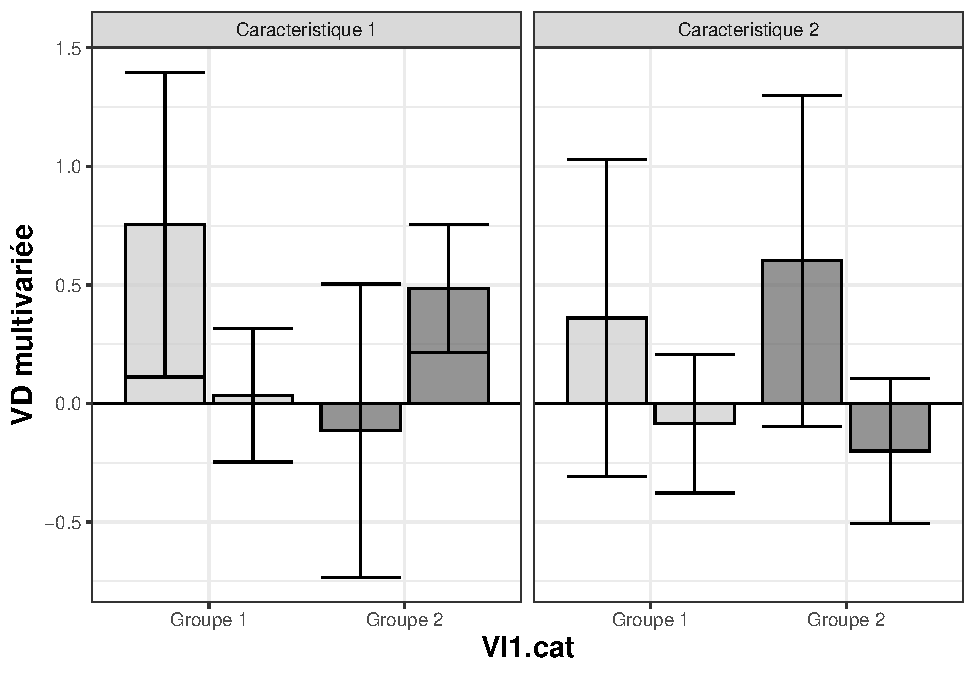
\includegraphics{Manuel_R_independant_files/figure-latex/unnamed-chunk-174-1.pdf}

\begin{Shaded}
\begin{Highlighting}[]
\NormalTok{my_data.manova.long <-}\StringTok{ }\NormalTok{my_data.manova }\OperatorTok
\StringTok{  }\KeywordTok{pivot_longer}\NormalTok{(}\DataTypeTok{cols =} \OperatorTok{-}\KeywordTok{c}\NormalTok{(VI1.cat, VI2.cat),}
               \DataTypeTok{names_to =} \StringTok{"VD"}\NormalTok{, }
               \DataTypeTok{values_to =} \StringTok{"VD.values"}\NormalTok{)}

\CommentTok{# graphique représentant les effets univariés}
\KeywordTok{ggplot}\NormalTok{(my_data.manova.long, }\KeywordTok{aes}\NormalTok{(}\DataTypeTok{x =}\NormalTok{ VI1.cat, }\DataTypeTok{y =}\NormalTok{ VD.values, }\DataTypeTok{fill =}\NormalTok{ VD)) }\OperatorTok{+}
\StringTok{  }\KeywordTok{geom_boxplot}\NormalTok{(}\DataTypeTok{color=}\StringTok{"black"}\NormalTok{, }\DataTypeTok{outlier.color=}\StringTok{"red"}\NormalTok{) }\OperatorTok{+}\StringTok{ }
\StringTok{  }\KeywordTok{facet_wrap}\NormalTok{(}\OperatorTok{~}\StringTok{ }\NormalTok{VI2.cat) }\OperatorTok{+}
\StringTok{  }\KeywordTok{ylab}\NormalTok{(}\StringTok{"Valeur de chaque VD"}\NormalTok{) }\OperatorTok{+}\StringTok{ }\KeywordTok{xlab}\NormalTok{(}\StringTok{"VI1.cat"}\NormalTok{) }\OperatorTok{+}\StringTok{ }
\StringTok{  }\KeywordTok{theme_bw}\NormalTok{() }\OperatorTok{+}\StringTok{ }
\StringTok{  }\KeywordTok{theme}\NormalTok{(}\DataTypeTok{axis.title.y =} \KeywordTok{element_text}\NormalTok{(}\DataTypeTok{size =} \DecValTok{14}\NormalTok{, }\DataTypeTok{hjust =} \FloatTok{0.5}\NormalTok{, }\DataTypeTok{face=}\StringTok{"bold"}\NormalTok{), }
        \DataTypeTok{axis.title.x =} \KeywordTok{element_text}\NormalTok{(}\DataTypeTok{face=}\StringTok{"bold"}\NormalTok{, }\DataTypeTok{size =} \DecValTok{14}\NormalTok{, }\DataTypeTok{hjust =} \FloatTok{0.5}\NormalTok{)) }\OperatorTok{+}
\StringTok{  }\KeywordTok{scale_fill_grey}\NormalTok{(}\DataTypeTok{start=}\FloatTok{0.8}\NormalTok{, }\DataTypeTok{end =} \FloatTok{0.4}\NormalTok{)}
\end{Highlighting}
\end{Shaded}

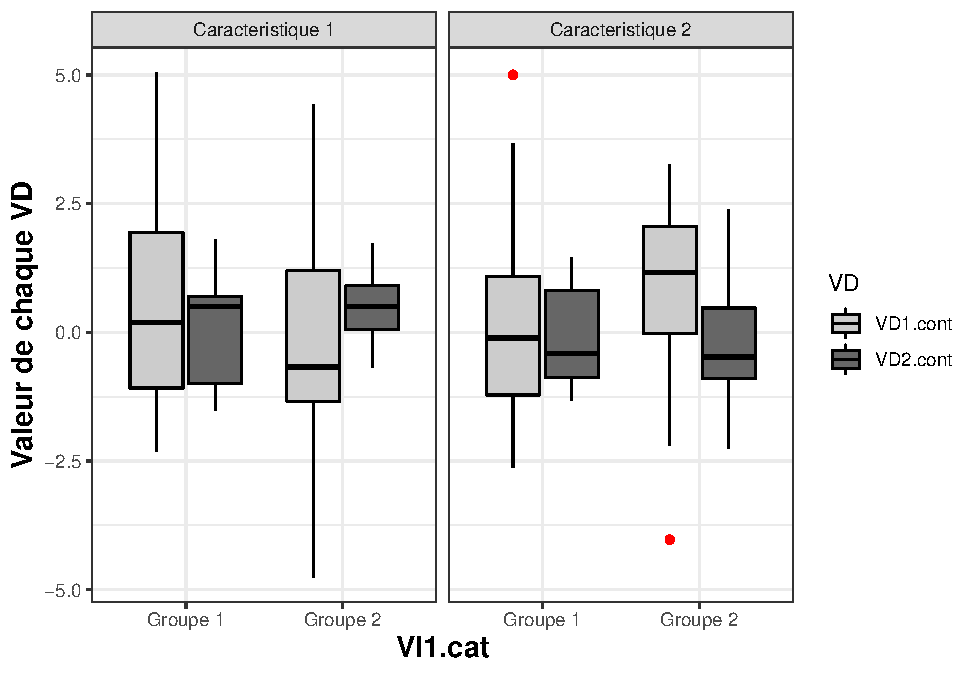
\includegraphics{Manuel_R_independant_files/figure-latex/unnamed-chunk-174-2.pdf}

\hypertarget{interpruxe9tation}{%
\subsubsection{Interprétation}\label{interpruxe9tation}}

{[}1{]} ``L'effet multivarié de l'interaction VI1.cat x VI2.cat sur VD1.cont et VD2.cont n'est pas significatif (F = 0.845, p = 0.436). Quelle que soit la variable dépendante ou la modalité de VI2.cat, l'effet de VI1.cat n'était pas significatif (toutes valeurs p non ajustées \textgreater{} 0.253)''

\hypertarget{regression-linuxe9aire-multivariuxe9e-1}{%
\subsection{Regression linéaire multivariée 1}\label{regression-linuxe9aire-multivariuxe9e-1}}

\hypertarget{type-de-variables-21}{%
\subsubsection{Type de variables}\label{type-de-variables-21}}

\textbf{Variables Dépendantes :} Numérique
\textbf{Variables Indépendantes :} Numériques

\hypertarget{packages-nuxe9cessaires-21}{%
\subsubsection{Packages nécessaires}\label{packages-nuxe9cessaires-21}}

\begin{Shaded}
\begin{Highlighting}[]
\KeywordTok{library}\NormalTok{(ggplot2)}
\KeywordTok{library}\NormalTok{(GGally)}
\KeywordTok{library}\NormalTok{(rstatix)}
\KeywordTok{library}\NormalTok{(dplyr)}
\KeywordTok{library}\NormalTok{(effects)}
\KeywordTok{library}\NormalTok{(tidyr)}
\end{Highlighting}
\end{Shaded}

\hypertarget{donnuxe9es-ruxe9elles-21}{%
\subsubsection{Données réelles}\label{donnuxe9es-ruxe9elles-21}}

\begin{Shaded}
\begin{Highlighting}[]
\CommentTok{# choisissez la ligne appropriée au format de votre fichier de données. }

\CommentTok{# si vos données sont dans un fichier .txt}
\NormalTok{regmultivariate1 <-}\StringTok{ }\KeywordTok{read.delim}\NormalTok{(}\KeywordTok{file.choose}\NormalTok{())}

\CommentTok{# si vos données sont dans un fichier .csv}
\NormalTok{regmultivariate1 <-}\StringTok{ }\KeywordTok{read.csv}\NormalTok{(}\KeywordTok{file.choose}\NormalTok{())}

\CommentTok{# si vos données sont dans un fichier .xls / .xlsx}
\NormalTok{regmultivariate1 <-}\StringTok{ }\KeywordTok{read_excel}\NormalTok{(}\KeywordTok{file.choose}\NormalTok{())}

\CommentTok{# une fois vos données chargées, vous pouvez renommer vos noms de colonnes afin qu'ils correspondent à ceux utilisés dans le code ci-dessous}
\CommentTok{# Si vous ne souhaitez pas renommer vos noms de colonnes, sautez cette étape mais adaptez le code des parties suivantes en lui indiquant les noms de colonnes de vos données.}

\CommentTok{# On crée une nouvelle colonne pour vos variables dépendantes continues (remplacez 'votre.nom.de.colonne' par les noms appropriés)}
\NormalTok{regmultivariate1}\OperatorTok{$}\NormalTok{VD1.cont <-}\StringTok{ }\NormalTok{regmultivariate1}\OperatorTok{$}\StringTok{'votre.nom.de.colonne'}
\NormalTok{regmultivariate1}\OperatorTok{$}\NormalTok{VD2.cont <-}\StringTok{ }\NormalTok{regmultivariate1}\OperatorTok{$}\StringTok{'votre.nom.de.colonne'}

\CommentTok{# On crée une nouvelle colonne pour vos variables indépendantes continues (remplacez 'votre.nom.de.colonne' par les noms appropriés)}
\NormalTok{regmultivariate1}\OperatorTok{$}\NormalTok{VI1.cont <-}\StringTok{ }\NormalTok{regmultivariate1}\OperatorTok{$}\StringTok{'votre.nom.de.colonne'}
\NormalTok{regmultivariate1}\OperatorTok{$}\NormalTok{VI2.cont <-}\StringTok{ }\NormalTok{regmultivariate1}\OperatorTok{$}\StringTok{'votre.nom.de.colonne'}
\end{Highlighting}
\end{Shaded}

\hypertarget{donnuxe9es-fictives-21}{%
\subsubsection{Données fictives}\label{donnuxe9es-fictives-21}}

\begin{Shaded}
\begin{Highlighting}[]
\KeywordTok{set.seed}\NormalTok{(}\DecValTok{4321}\NormalTok{)}
\NormalTok{regmultivariate1 <-}\StringTok{ }\KeywordTok{rnorm}\NormalTok{(}\DecValTok{65}\NormalTok{)}\OperatorTok{*}\DecValTok{3}
\NormalTok{my_data.regmultivariate1 <-}\StringTok{ }\KeywordTok{data.frame}\NormalTok{(}
  \DataTypeTok{VD1.cont =} \KeywordTok{rnorm}\NormalTok{(}\DecValTok{65}\NormalTok{) }\OperatorTok{+}\StringTok{ }\DecValTok{1}\OperatorTok{*}\NormalTok{regmultivariate1,}
  \DataTypeTok{VD2.cont =} \KeywordTok{rnorm}\NormalTok{(}\DecValTok{65}\NormalTok{) }\OperatorTok{+}\StringTok{ }\FloatTok{0.2}\OperatorTok{*}\NormalTok{regmultivariate1,}
  \DataTypeTok{VI1.cont =} \KeywordTok{rnorm}\NormalTok{(}\DecValTok{65}\NormalTok{)}\OperatorTok{+}\StringTok{ }\FloatTok{0.2}\OperatorTok{*}\NormalTok{regmultivariate1)}
\end{Highlighting}
\end{Shaded}

\hypertarget{duxe9claration-du-type-de-variables-20}{%
\subsubsection{Déclaration du type de variables}\label{duxe9claration-du-type-de-variables-20}}

\begin{Shaded}
\begin{Highlighting}[]
\NormalTok{my_data.regmultivariate1}\OperatorTok{$}\NormalTok{VD1.cont <-}\StringTok{ }\KeywordTok{as.numeric}\NormalTok{(}\KeywordTok{as.character}\NormalTok{(my_data.regmultivariate1}\OperatorTok{$}\NormalTok{VD1.cont))}
\NormalTok{my_data.regmultivariate1}\OperatorTok{$}\NormalTok{VD2.cont <-}\StringTok{ }\KeywordTok{as.numeric}\NormalTok{(}\KeywordTok{as.character}\NormalTok{(my_data.regmultivariate1}\OperatorTok{$}\NormalTok{VD2.cont))}
\NormalTok{my_data.regmultivariate1}\OperatorTok{$}\NormalTok{VI1.cont <-}\StringTok{ }\KeywordTok{as.numeric}\NormalTok{(}\KeywordTok{as.character}\NormalTok{(my_data.regmultivariate1}\OperatorTok{$}\NormalTok{VI1.cont))}
\end{Highlighting}
\end{Shaded}

\hypertarget{inspection-des-donnuxe9es-20}{%
\subsubsection{Inspection des données}\label{inspection-des-donnuxe9es-20}}

\begin{Shaded}
\begin{Highlighting}[]
\CommentTok{## Les graphiques situés sur la diagonale représentent la distribution des variables}
\CommentTok{## Les graphiques (ou les valeurs de corrélation) situés au dessus et en dessous de la diagonale représentent l'association entre les différentes variables}
\KeywordTok{ggpairs}\NormalTok{(my_data.regmultivariate1,}
        \DataTypeTok{lower =} \KeywordTok{list}\NormalTok{(}\DataTypeTok{continuous =} \KeywordTok{wrap}\NormalTok{(}\StringTok{"smooth"}\NormalTok{, }\DataTypeTok{alpha =} \FloatTok{0.7}\NormalTok{), }\DataTypeTok{combo =} \StringTok{"box_no_facet"}\NormalTok{),}
        \DataTypeTok{upper =} \KeywordTok{list}\NormalTok{(}\DataTypeTok{combo =} \StringTok{"facetdensity"}\NormalTok{, }\DataTypeTok{discrete =} \StringTok{"facetbar"}\NormalTok{), }
        \DataTypeTok{mapping =} \KeywordTok{aes}\NormalTok{(}\DataTypeTok{alpha =} \FloatTok{0.8}\NormalTok{)) }\OperatorTok{+}\StringTok{ }\KeywordTok{theme_bw}\NormalTok{()}
\end{Highlighting}
\end{Shaded}

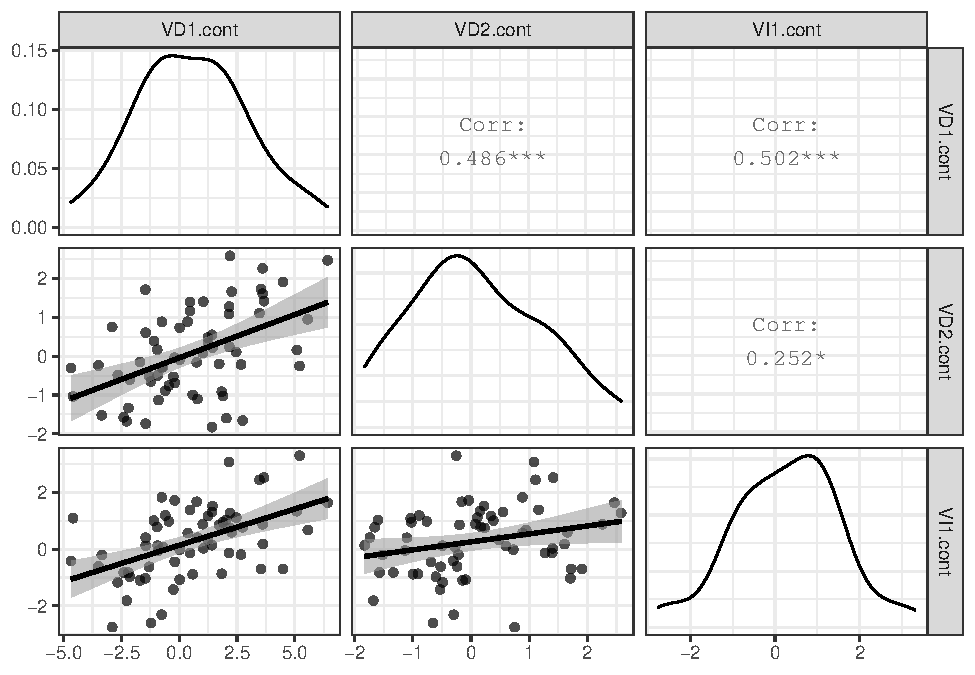
\includegraphics{Manuel_R_independant_files/figure-latex/unnamed-chunk-180-1.pdf}

\hypertarget{analyse-des-donnuxe9es-21}{%
\subsubsection{Analyse des données}\label{analyse-des-donnuxe9es-21}}

\begin{Shaded}
\begin{Highlighting}[]
\CommentTok{# calcul de la régression multivariée et stockage des résultats dans l’objet regmultivariate1.test}
\NormalTok{regmultivariate1.test <-}\StringTok{ }\KeywordTok{lm}\NormalTok{(}\DataTypeTok{formula =} \KeywordTok{cbind}\NormalTok{(VD1.cont, VD2.cont) }\OperatorTok{~}\StringTok{ }\NormalTok{VI1.cont,}
                    \DataTypeTok{data =}\NormalTok{ my_data.regmultivariate1)}

\CommentTok{# obtention des résultats de la régression linéaire multivariée}

\CommentTok{# effet multivarié}
\KeywordTok{Anova}\NormalTok{(regmultivariate1.test)}
\end{Highlighting}
\end{Shaded}

\begin{verbatim}
## 
## Type II MANOVA Tests: Pillai test statistic
##          Df test stat approx F num Df den Df    Pr(>F)    
## VI1.cont  1    0.2523   10.461      2     62 0.0001218 ***
## ---
## Signif. codes:  0 '***' 0.001 '**' 0.01 '*' 0.05 '.' 0.1 ' ' 1
\end{verbatim}

\begin{Shaded}
\begin{Highlighting}[]
\CommentTok{# effet univarié}
\KeywordTok{summary}\NormalTok{(regmultivariate1.test)}
\end{Highlighting}
\end{Shaded}

\begin{verbatim}
## Response VD1.cont :
## 
## Call:
## lm(formula = VD1.cont ~ VI1.cont, data = my_data.regmultivariate1)
## 
## Residuals:
##     Min      1Q  Median      3Q     Max 
## -5.9440 -1.3316 -0.1302  1.0871  4.9018 
## 
## Coefficients:
##             Estimate Std. Error t value Pr(>|t|)    
## (Intercept)   0.2786     0.2709   1.028    0.308    
## VI1.cont      0.9833     0.2133   4.610 2.02e-05 ***
## ---
## Signif. codes:  0 '***' 0.001 '**' 0.01 '*' 0.05 '.' 0.1 ' ' 1
## 
## Residual standard error: 2.13 on 63 degrees of freedom
## Multiple R-squared:  0.2522,	Adjusted R-squared:  0.2403 
## F-statistic: 21.25 on 1 and 63 DF,  p-value: 2.021e-05
## 
## 
## Response VD2.cont :
## 
## Call:
## lm(formula = VD2.cont ~ VI1.cont, data = my_data.regmultivariate1)
## 
## Residuals:
##     Min      1Q  Median      3Q     Max 
## -1.8773 -0.7352 -0.1386  0.7147  2.2754 
## 
## Coefficients:
##             Estimate Std. Error t value Pr(>|t|)  
## (Intercept)  0.01706    0.13886   0.123   0.9026  
## VI1.cont     0.22598    0.10935   2.067   0.0429 *
## ---
## Signif. codes:  0 '***' 0.001 '**' 0.01 '*' 0.05 '.' 0.1 ' ' 1
## 
## Residual standard error: 1.092 on 63 degrees of freedom
## Multiple R-squared:  0.06349,	Adjusted R-squared:  0.04862 
## F-statistic: 4.271 on 1 and 63 DF,  p-value: 0.04288
\end{verbatim}

\hypertarget{graphique-21}
\NormalTok{crude.slope.regmultivariate1 <-}\StringTok{ }\KeywordTok{do.call}\NormalTok{(rbind,}
  \KeywordTok{as.data.frame}\NormalTok{(}
    \KeywordTok{effect}\NormalTok{(}
      \DataTypeTok{term =} \StringTok{"VI1.cont"}\NormalTok{, }
      \DataTypeTok{mod =}\NormalTok{ regmultivariate1.test)))}

\NormalTok{crude.slope.regmultivariate1}\OperatorTok{$}\NormalTok{Outcome <-}\StringTok{ }\KeywordTok{rep}\NormalTok{(}\KeywordTok{c}\NormalTok{(}\StringTok{"VD1.cont"}\NormalTok{, }\StringTok{"VD2.cont"}\NormalTok{), }\DataTypeTok{each =} \KeywordTok{nrow}\NormalTok{(crude.slope.regmultivariate1)}\OperatorTok{/}\DecValTok{2}\NormalTok{)}

\NormalTok{my_data.regmultivariate1.long <-}\StringTok{ }\NormalTok{my_data.regmultivariate1 }\OperatorTok\StringTok{ }
\StringTok{  }\KeywordTok{pivot_longer}\NormalTok{(}\DataTypeTok{cols =} \KeywordTok{c}\NormalTok{(VD1.cont, VD2.cont),}
               \DataTypeTok{names_to =} \StringTok{"VD.names"}\NormalTok{,}
               \DataTypeTok{values_to =} \StringTok{"VD"}\NormalTok{)}


\KeywordTok{ggplot}\NormalTok{() }\OperatorTok{+}
\StringTok{  }\KeywordTok{geom_point}\NormalTok{(}\DataTypeTok{data =}\NormalTok{ my_data.regmultivariate1.long, }
       \KeywordTok{aes}\NormalTok{(}\DataTypeTok{x =}\NormalTok{ VI1.cont, }\DataTypeTok{y =}\NormalTok{ VD, }\DataTypeTok{color =}\NormalTok{ VD.names),}
       \DataTypeTok{size =} \DecValTok{3}\NormalTok{, }\DataTypeTok{alpha =} \FloatTok{0.4}\NormalTok{) }\OperatorTok{+}\StringTok{ }
\StringTok{  }\KeywordTok{geom_ribbon}\NormalTok{(}\DataTypeTok{data =}\NormalTok{ crude.slope.regmultivariate1, }
         \KeywordTok{aes}\NormalTok{(}\DataTypeTok{x =}\NormalTok{ VI1.cont, }\DataTypeTok{y =}\NormalTok{ fit, }
             \DataTypeTok{fill =}\NormalTok{ Outcome,}
             \DataTypeTok{ymin =}\NormalTok{ lower, }\DataTypeTok{ymax =}\NormalTok{ upper), }
         \DataTypeTok{alpha=}\FloatTok{0.7}\NormalTok{) }\OperatorTok{+}
\StringTok{  }\KeywordTok{geom_line}\NormalTok{(}\DataTypeTok{data =}\NormalTok{ crude.slope.regmultivariate1, }
        \KeywordTok{aes}\NormalTok{(}\DataTypeTok{x =}\NormalTok{ VI1.cont , }\DataTypeTok{y =}\NormalTok{ fit, }\DataTypeTok{color =}\NormalTok{ Outcome), }
        \DataTypeTok{size =} \DecValTok{1}\NormalTok{) }\OperatorTok{+}
\StringTok{  }\KeywordTok{ylab}\NormalTok{(}\StringTok{"VD1.cont"}\NormalTok{) }\OperatorTok{+}\StringTok{ }\KeywordTok{xlab}\NormalTok{(}\StringTok{"VI1.cont"}\NormalTok{) }\OperatorTok{+}\StringTok{ }
\StringTok{  }\KeywordTok{theme_bw}\NormalTok{() }\OperatorTok{+}\StringTok{ }
\StringTok{  }\KeywordTok{theme}\NormalTok{(}\DataTypeTok{axis.title.y =} \KeywordTok{element_text}\NormalTok{(}\DataTypeTok{size =} \DecValTok{14}\NormalTok{, }\DataTypeTok{hjust =} \FloatTok{0.5}\NormalTok{, }\DataTypeTok{face=}\StringTok{"bold"}\NormalTok{), }
        \DataTypeTok{axis.title.x =} \KeywordTok{element_text}\NormalTok{(}\DataTypeTok{face=}\StringTok{"bold"}\NormalTok{, }\DataTypeTok{size =} \DecValTok{14}\NormalTok{, }\DataTypeTok{hjust =} \FloatTok{0.5}\NormalTok{)) }\OperatorTok{+}
\StringTok{  }\KeywordTok{scale_color_manual}\NormalTok{(}\DataTypeTok{values =} \KeywordTok{c}\NormalTok{(}\StringTok{"black"}\NormalTok{, }\StringTok{"red"}\NormalTok{)) }\OperatorTok{+}
\StringTok{  }\KeywordTok{scale_fill_manual}\NormalTok{(}\DataTypeTok{values =} \KeywordTok{c}\NormalTok{(}\StringTok{"lightgrey"}\NormalTok{, }\StringTok{"#FDA2A2"}\NormalTok{)) }\OperatorTok{+}
\StringTok{  }\KeywordTok{guides}\NormalTok{(}\DataTypeTok{fill=}\OtherTok{FALSE}\NormalTok{)}
\end{Highlighting}
\end{Shaded}

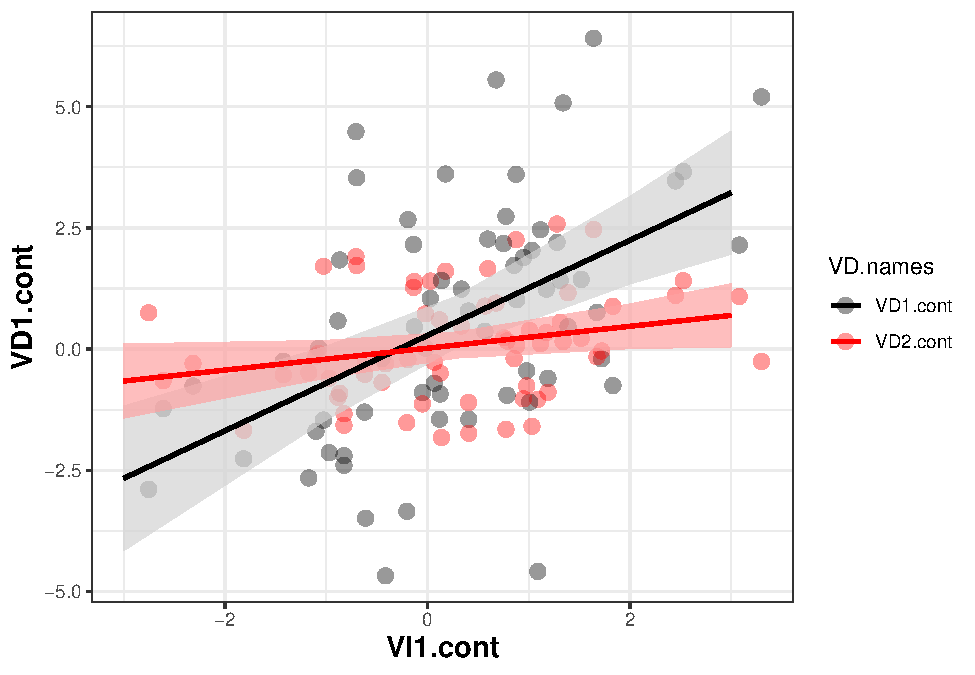
\includegraphics{Manuel_R_independant_files/figure-latex/unnamed-chunk-182-1.pdf}

\hypertarget{interpruxe9tation-1}{%
\subsubsection{Interprétation}\label{interpruxe9tation-1}}

{[}1{]} ``L'effet multivarié de VI1.cont sur VD1.cont et VD2.cont est statistiquement significatif (F = 10.461, p = 0.000122). Quelle que soit la variable dépendante, l'effet univarié de VI1.cont était significatif ou marginalement significatif (toutes valeurs p non ajustées \textless{} 0.0429)''

\hypertarget{mancova}{%
\subsection{MANCOVA}\label{mancova}}

\textbf{ATTENTION :} si votre variable indépendante principale est \textbf{Numérique} OU que vous faites une hypothèse d'interaction entre votre VI principale catégorielle et une autre covariable, reportez-vous à la section suivante \textbf{Régression linéaire multivariée 2}.

Dans le cas contraire (votre VI principale est catégorielle ET vous ne faites pas d'hypothèse d'interaction entre votre VI catégorielle et une covariable), utilisez une MANCOVA décrite dans cette vignette.

\hypertarget{type-de-variables-22}{%
\subsubsection{Type de variables}\label{type-de-variables-22}}

\textbf{Variables Dépendantes :} Numériques
\textbf{Variable indépendante principale:} Catégorielle
\textbf{Autres variables indépendantes (covariables) :} Numériques / Catégorielles

\hypertarget{packages-nuxe9cessaires-22}{%
\subsubsection{Packages nécessaires}\label{packages-nuxe9cessaires-22}}

\begin{Shaded}
\begin{Highlighting}[]
\KeywordTok{library}\NormalTok{(ggplot2)}
\KeywordTok{library}\NormalTok{(GGally)}
\KeywordTok{library}\NormalTok{(rstatix)}
\KeywordTok{library}\NormalTok{(dplyr)}
\KeywordTok{library}\NormalTok{(effects)}
\KeywordTok{library}\NormalTok{(forcats)}
\KeywordTok{library}\NormalTok{(emmeans)}
\KeywordTok{library}\NormalTok{(tidyr)}
\end{Highlighting}
\end{Shaded}

\hypertarget{donnuxe9es-ruxe9elles-22}{%
\subsubsection{Données réelles}\label{donnuxe9es-ruxe9elles-22}}

\begin{Shaded}
\begin{Highlighting}[]
\CommentTok{# choisissez la ligne appropriée au format de votre fichier de données. }

\CommentTok{# si vos données sont dans un fichier .txt}
\NormalTok{my_data.mancova <-}\StringTok{ }\KeywordTok{read.delim}\NormalTok{(}\KeywordTok{file.choose}\NormalTok{())}

\CommentTok{# si vos données sont dans un fichier .csv}
\NormalTok{my_data.mancova <-}\StringTok{ }\KeywordTok{read.csv}\NormalTok{(}\KeywordTok{file.choose}\NormalTok{())}

\CommentTok{# si vos données sont dans un fichier .xls / .xlsx}
\NormalTok{my_data.mancova <-}\StringTok{ }\KeywordTok{read_excel}\NormalTok{(}\KeywordTok{file.choose}\NormalTok{())}

\CommentTok{# une fois vos données chargées, vous pouvez renommer vos noms de colonnes afin qu'ils correspondent à ceux utilisés dans le code ci-dessous}
\CommentTok{# Si vous ne souhaitez pas renommer vos noms de colonnes, sautez cette étape mais adaptez le code des parties suivantes en lui indiquant les noms de colonnes de vos données.}

\CommentTok{# On crée une nouvelle colonne pour vos variables dépendantes continues (remplacez 'votre.nom.de.colonne' par les noms appropriés)}
\NormalTok{my_data.mancova}\OperatorTok{$}\NormalTok{VD1.cont <-}\StringTok{ }\NormalTok{my_data.mancova}\OperatorTok{$}\StringTok{'votre.nom.de.colonne'}
\NormalTok{my_data.mancova}\OperatorTok{$}\NormalTok{VD2.cont <-}\StringTok{ }\NormalTok{my_data.mancova}\OperatorTok{$}\StringTok{'votre.nom.de.colonne'}

\CommentTok{# On crée une nouvelle colonne pour votre variable indépendante catégorielle (remplacez 'votre.nom.de.colonne' par le nom approprié)}
\NormalTok{my_data.mancova}\OperatorTok{$}\NormalTok{VI1.cat <-}\StringTok{ }\NormalTok{my_data.mancova}\OperatorTok{$}\StringTok{'votre.nom.de.colonne'}

\CommentTok{# On crée une nouvelle colonne pour votre variable indépendante continue (remplacez 'votre.nom.de.colonne' par le nom approprié)}
\NormalTok{my_data.mancova}\OperatorTok{$}\NormalTok{VI1.cont <-}\StringTok{ }\NormalTok{my_data.mancova}\OperatorTok{$}\StringTok{'votre.nom.de.colonne'}
\end{Highlighting}
\end{Shaded}

\hypertarget{donnuxe9es-fictives-22}{%
\subsubsection{Données fictives}\label{donnuxe9es-fictives-22}}

\begin{Shaded}
\begin{Highlighting}[]
\KeywordTok{set.seed}\NormalTok{(}\DecValTok{4321}\NormalTok{)}
\NormalTok{mancova <-}\StringTok{ }\KeywordTok{rnorm}\NormalTok{(}\DecValTok{50}\NormalTok{)}
\NormalTok{my_data.mancova <-}\StringTok{ }\KeywordTok{data.frame}\NormalTok{(}
  \DataTypeTok{VD1.cont =} \KeywordTok{rnorm}\NormalTok{(}\DecValTok{50}\NormalTok{)}\OperatorTok{*}\DecValTok{2} \OperatorTok{+}\StringTok{ }\DecValTok{1}\OperatorTok{*}\NormalTok{mancova,}
  \DataTypeTok{VD2.cont =} \KeywordTok{rnorm}\NormalTok{(}\DecValTok{50}\NormalTok{)}\OperatorTok{+}\StringTok{ }\FloatTok{0.2}\OperatorTok{*}\NormalTok{mancova,}
  \DataTypeTok{VI1.cat =} \KeywordTok{rbinom}\NormalTok{(}\DecValTok{50}\NormalTok{, }\DecValTok{1}\NormalTok{, }\FloatTok{0.5}\NormalTok{) }\OperatorTok{+}\StringTok{ }\DecValTok{1}\NormalTok{,}
  \DataTypeTok{VI2.cont =} \KeywordTok{rnorm}\NormalTok{(}\DecValTok{50}\NormalTok{)}\OperatorTok{+}\StringTok{ }\FloatTok{0.6}\OperatorTok{*}\NormalTok{mancova)}

\NormalTok{my_data.mancova}\OperatorTok{$}\NormalTok{VI1.cat <-}\StringTok{ }\KeywordTok{fct_recode}\NormalTok{(}\KeywordTok{factor}\NormalTok{(my_data.mancova}\OperatorTok{$}\NormalTok{VI1.cat), }
          \StringTok{"Groupe 1"}\NormalTok{ =}\StringTok{ "1"}\NormalTok{, }
          \StringTok{"Groupe 2"}\NormalTok{ =}\StringTok{ "2"}\NormalTok{) }
\end{Highlighting}
\end{Shaded}

\hypertarget{duxe9claration-du-type-de-variables-21}{%
\subsubsection{Déclaration du type de variables}\label{duxe9claration-du-type-de-variables-21}}

\begin{Shaded}
\begin{Highlighting}[]
\NormalTok{my_data.mancova}\OperatorTok{$}\NormalTok{VD1.cont <-}\StringTok{ }\KeywordTok{as.numeric}\NormalTok{(}\KeywordTok{as.character}\NormalTok{(my_data.mancova}\OperatorTok{$}\NormalTok{VD1.cont))}
\NormalTok{my_data.mancova}\OperatorTok{$}\NormalTok{VD2.cont <-}\StringTok{ }\KeywordTok{as.numeric}\NormalTok{(}\KeywordTok{as.character}\NormalTok{(my_data.mancova}\OperatorTok{$}\NormalTok{VD2.cont))}
\NormalTok{my_data.mancova}\OperatorTok{$}\NormalTok{VI1.cat <-}\StringTok{ }\KeywordTok{factor}\NormalTok{(my_data.mancova}\OperatorTok{$}\NormalTok{VI1.cat)}
\NormalTok{my_data.mancova}\OperatorTok{$}\NormalTok{VI2.cont <-}\StringTok{ }\KeywordTok{as.numeric}\NormalTok{(}\KeywordTok{as.character}\NormalTok{(my_data.mancova}\OperatorTok{$}\NormalTok{VI2.cont))}
\end{Highlighting}
\end{Shaded}

\hypertarget{inspection-des-donnuxe9es-21}{%
\subsubsection{Inspection des données}\label{inspection-des-donnuxe9es-21}}

\begin{Shaded}
\begin{Highlighting}[]
\CommentTok{## Les graphiques situés sur la diagonale représentent la distribution des variables}
\CommentTok{## Les graphiques (ou les valeurs de corrélation) situés au dessus et en dessous de la diagonale représentent l'association entre les différentes variables}
\KeywordTok{ggpairs}\NormalTok{(my_data.mancova,}
        \DataTypeTok{lower =} \KeywordTok{list}\NormalTok{(}\DataTypeTok{continuous =} \KeywordTok{wrap}\NormalTok{(}\StringTok{"smooth"}\NormalTok{, }\DataTypeTok{alpha =} \FloatTok{0.7}\NormalTok{), }\DataTypeTok{combo =} \StringTok{"box_no_facet"}\NormalTok{),}
        \DataTypeTok{upper =} \KeywordTok{list}\NormalTok{(}\DataTypeTok{combo =} \StringTok{"facetdensity"}\NormalTok{, }\DataTypeTok{discrete =} \StringTok{"facetbar"}\NormalTok{), }
        \DataTypeTok{mapping =} \KeywordTok{aes}\NormalTok{(}\DataTypeTok{alpha =} \FloatTok{0.8}\NormalTok{)) }\OperatorTok{+}\StringTok{ }\KeywordTok{theme_bw}\NormalTok{()}
\end{Highlighting}
\end{Shaded}

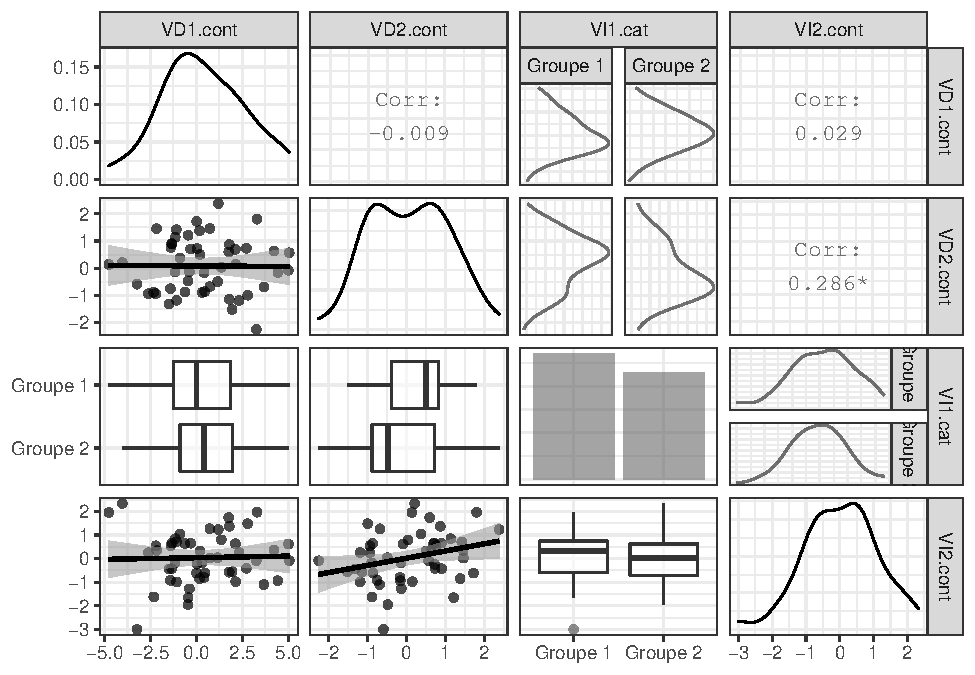
\includegraphics{Manuel_R_independant_files/figure-latex/unnamed-chunk-188-1.pdf}

\hypertarget{analyse-des-donnuxe9es-22}{%
\subsubsection{Analyse des données}\label{analyse-des-donnuxe9es-22}}

\begin{Shaded}
\begin{Highlighting}[]
\CommentTok{# calcul de la mancova et stockage des résultats dans l’objet mancova.test}
\NormalTok{mancova.test <-}\StringTok{ }\KeywordTok{lm}\NormalTok{(}\DataTypeTok{formula =} \KeywordTok{cbind}\NormalTok{(VD1.cont, VD2.cont) }\OperatorTok{~}\StringTok{ }\NormalTok{VI1.cat }\OperatorTok{+}\StringTok{ }\NormalTok{VI2.cont,}
                 \DataTypeTok{data =}\NormalTok{ my_data.mancova)}

\CommentTok{# obtention des résultats de la mancova}

\CommentTok{## résultats multivariés }
\KeywordTok{Anova}\NormalTok{(mancova.test)}
\end{Highlighting}
\end{Shaded}

\begin{verbatim}
## 
## Type II MANOVA Tests: Pillai test statistic
##          Df test stat approx F num Df den Df Pr(>F)
## VI1.cat   1  0.042032   1.0091      2     46 0.3725
## VI2.cont  1  0.082378   2.0648      2     46 0.1384
\end{verbatim}

\begin{Shaded}
\begin{Highlighting}[]
\CommentTok{## résultats univariés }
\KeywordTok{summary}\NormalTok{(mancova.test)}
\end{Highlighting}
\end{Shaded}

\begin{verbatim}
## Response VD1.cont :
## 
## Call:
## lm(formula = VD1.cont ~ VI1.cat + VI2.cont, data = my_data.mancova)
## 
## Residuals:
##     Min      1Q  Median      3Q     Max 
## -5.1823 -1.5719 -0.2031  1.5844  4.7531 
## 
## Coefficients:
##                 Estimate Std. Error t value Pr(>|t|)
## (Intercept)      0.29885    0.44581   0.670    0.506
## VI1.catGroupe 2  0.17677    0.65682   0.269    0.789
## VI2.cont         0.06324    0.30540   0.207    0.837
## 
## Residual standard error: 2.314 on 47 degrees of freedom
## Multiple R-squared:  0.002376,	Adjusted R-squared:  -0.04008 
## F-statistic: 0.05597 on 2 and 47 DF,  p-value: 0.9456
## 
## 
## Response VD2.cont :
## 
## Call:
## lm(formula = VD2.cont ~ VI1.cat + VI2.cont, data = my_data.mancova)
## 
## Residuals:
##      Min       1Q   Median       3Q      Max 
## -2.09123 -0.68646 -0.07975  0.62216  2.19576 
## 
## Coefficients:
##                 Estimate Std. Error t value Pr(>|t|)  
## (Intercept)       0.2491     0.1876   1.328   0.1908  
## VI1.catGroupe 2  -0.3907     0.2764  -1.413   0.1642  
## VI2.cont          0.2624     0.1285   2.041   0.0468 *
## ---
## Signif. codes:  0 '***' 0.001 '**' 0.01 '*' 0.05 '.' 0.1 ' ' 1
## 
## Residual standard error: 0.9738 on 47 degrees of freedom
## Multiple R-squared:  0.119,	Adjusted R-squared:  0.08156 
## F-statistic: 3.176 on 2 and 47 DF,  p-value: 0.05086
\end{verbatim}

\hypertarget{graphique-22}{%
\subsubsection{Graphique}\label{graphique-22}}

\begin{Shaded}
\begin{Highlighting}[]
\CommentTok{# graphique représentant les effets multivariés}
\NormalTok{adjusted.mancova <-}\StringTok{ }\KeywordTok{do.call}\NormalTok{(rbind, }\KeywordTok{data.frame}\NormalTok{(}\KeywordTok{effect}\NormalTok{(}\DataTypeTok{term=}\StringTok{"VI1.cat"}\NormalTok{, }\DataTypeTok{mod=}\NormalTok{ mancova.test)))}
\NormalTok{adjusted.mancova}\OperatorTok{$}\NormalTok{Outcome <-}\StringTok{ }\KeywordTok{rep}\NormalTok{(}\KeywordTok{c}\NormalTok{(}\StringTok{"VD1.cont"}\NormalTok{, }\StringTok{"VD2.cont"}\NormalTok{), }\DataTypeTok{each =} \KeywordTok{nrow}\NormalTok{(adjusted.mancova)}\OperatorTok{/}\DecValTok{2}\NormalTok{)}

\KeywordTok{ggplot}\NormalTok{(adjusted.mancova, }
       \KeywordTok{aes}\NormalTok{(}\DataTypeTok{x =}\NormalTok{ VI1.cat, }\DataTypeTok{y =}\NormalTok{ fit, }\DataTypeTok{fill =}\NormalTok{ VI1.cat)) }\OperatorTok{+}
\StringTok{  }\KeywordTok{geom_hline}\NormalTok{(}\KeywordTok{aes}\NormalTok{(}\DataTypeTok{yintercept =} \DecValTok{0}\NormalTok{)) }\OperatorTok{+}\StringTok{ }
\StringTok{  }\KeywordTok{geom_bar}\NormalTok{(}\DataTypeTok{stat =} \StringTok{"identity"}\NormalTok{, }\DataTypeTok{color =} \StringTok{"black"}\NormalTok{, }\DataTypeTok{alpha =} \FloatTok{0.7}\NormalTok{,}
           \DataTypeTok{position =} \KeywordTok{position_dodge2}\NormalTok{()) }\OperatorTok{+}
\StringTok{  }\KeywordTok{geom_errorbar}\NormalTok{(}\KeywordTok{aes}\NormalTok{(}\DataTypeTok{ymin =}\NormalTok{ fit }\OperatorTok{-}\StringTok{ }\NormalTok{se, }
                    \DataTypeTok{ymax =}\NormalTok{ fit }\OperatorTok{+}\StringTok{ }\NormalTok{se), }
                \DataTypeTok{width =} \FloatTok{0.1}\NormalTok{,}
                \DataTypeTok{position =} \KeywordTok{position_dodge2}\NormalTok{(}\DataTypeTok{width =} \FloatTok{0.9}\NormalTok{), }
                \DataTypeTok{color =} \StringTok{"black"}\NormalTok{) }\OperatorTok{+}
\StringTok{  }\KeywordTok{facet_wrap}\NormalTok{(}\OperatorTok{~}\StringTok{ }\NormalTok{Outcome) }\OperatorTok{+}
\StringTok{  }\KeywordTok{ylab}\NormalTok{(}\StringTok{"VD multivariée"}\NormalTok{) }\OperatorTok{+}\StringTok{ }\KeywordTok{xlab}\NormalTok{(}\StringTok{"VI1.cat"}\NormalTok{) }\OperatorTok{+}\StringTok{ }
\StringTok{  }\KeywordTok{theme_bw}\NormalTok{() }\OperatorTok{+}\StringTok{ }
\StringTok{  }\KeywordTok{theme}\NormalTok{(}\DataTypeTok{axis.title.y =} \KeywordTok{element_text}\NormalTok{(}\DataTypeTok{size =} \DecValTok{14}\NormalTok{, }\DataTypeTok{hjust =} \FloatTok{0.5}\NormalTok{, }\DataTypeTok{face=}\StringTok{"bold"}\NormalTok{), }
        \DataTypeTok{axis.title.x =} \KeywordTok{element_text}\NormalTok{(}\DataTypeTok{face=}\StringTok{"bold"}\NormalTok{, }\DataTypeTok{size =} \DecValTok{14}\NormalTok{, }\DataTypeTok{hjust =} \FloatTok{0.5}\NormalTok{)) }\OperatorTok{+}\StringTok{ }
\StringTok{  }\KeywordTok{scale_fill_grey}\NormalTok{(}\DataTypeTok{start=}\FloatTok{0.8}\NormalTok{, }\DataTypeTok{end =} \FloatTok{0.4}\NormalTok{) }\OperatorTok{+}\StringTok{ }
\StringTok{  }\KeywordTok{guides}\NormalTok{(}\DataTypeTok{fill=}\OtherTok{FALSE}\NormalTok{)}
\end{Highlighting}
\end{Shaded}

\includegraphics{Manuel_R_independant_files/figure-latex/unnamed-chunk-190-1.pdf}

\hypertarget{interpruxe9tation-2}{%
\subsubsection{Interprétation}\label{interpruxe9tation-2}}

{[}1{]} ``L'effet multivarié de VI1.cat sur VD1.cont et VD2.cont n'est pas significatif (F = 1.009, p = 0.372). Plus précisément, l'effet univarié de VI1.cat était non significatif sur VD1.cont (b = 0.177, SE = 0.657, p = 0.789), et sur VD2.cont (b = -0.391, SE = 0.276, p = 0.164)''

\hypertarget{regression-linuxe9aire-multivariuxe9e-2}{%
\subsection{Regression linéaire multivariée 2}\label{regression-linuxe9aire-multivariuxe9e-2}}

\textbf{ATTENTION :} si votre variable indépendante principale est \textbf{catégorielle} ET que vous ne faites pas d'hypothèse d'interaction entre cette VI principale catégorielle et une autre covariable, reportez-vous à la section précédente \textbf{MANCOVA}.

Dans le cas contraire (votre VI principale est numérique OU vous faites une hypothèse d'interaction entre votre VI catégorielle et une covariable), utilisez une régression linéaire multivariée décrite dans cette vignette.

\hypertarget{type-de-variables-23}{%
\subsubsection{Type de variables}\label{type-de-variables-23}}

\textbf{Variables Dépendantes :} Numérique
\textbf{Variables Indépendantes :} Numérique / Catégorielles

\hypertarget{packages-nuxe9cessaires-23}{%
\subsubsection{Packages nécessaires}\label{packages-nuxe9cessaires-23}}

\begin{Shaded}
\begin{Highlighting}[]
\KeywordTok{library}\NormalTok{(ggplot2)}
\KeywordTok{library}\NormalTok{(GGally)}
\KeywordTok{library}\NormalTok{(rstatix)}
\KeywordTok{library}\NormalTok{(dplyr)}
\KeywordTok{library}\NormalTok{(effects)}
\KeywordTok{library}\NormalTok{(tidyr)}
\KeywordTok{library}\NormalTok{(effects)}
\end{Highlighting}
\end{Shaded}

\hypertarget{donnuxe9es-ruxe9elles-23}{%
\subsubsection{Données réelles}\label{donnuxe9es-ruxe9elles-23}}

\begin{Shaded}
\begin{Highlighting}[]
\CommentTok{# choisissez la ligne appropriée au format de votre fichier de données. }

\CommentTok{# si vos données sont dans un fichier .txt}
\NormalTok{my_data.regmultivariate2 <-}\StringTok{ }\KeywordTok{read.delim}\NormalTok{(}\KeywordTok{file.choose}\NormalTok{())}

\CommentTok{# si vos données sont dans un fichier .csv}
\NormalTok{my_data.regmultivariate2 <-}\StringTok{ }\KeywordTok{read.csv}\NormalTok{(}\KeywordTok{file.choose}\NormalTok{())}

\CommentTok{# si vos données sont dans un fichier .xls / .xlsx}
\NormalTok{my_data.regmultivariate2 <-}\StringTok{ }\KeywordTok{read_excel}\NormalTok{(}\KeywordTok{file.choose}\NormalTok{())}

\CommentTok{# une fois vos données chargées, vous pouvez renommer vos noms de colonnes afin qu'ils correspondent à ceux utilisés dans le code ci-dessous}
\CommentTok{# Si vous ne souhaitez pas renommer vos noms de colonnes, sautez cette étape mais adaptez le code des parties suivantes en lui indiquant les noms de colonnes de vos données.}

\CommentTok{# On crée une nouvelle colonne pour vos variables dépendantes continues (remplacez 'votre.nom.de.colonne' par les noms appropriés)}
\NormalTok{my_data.regmultivariate2}\OperatorTok{$}\NormalTok{VD1.cont <-}\StringTok{ }\NormalTok{my_data.regmultivariate2}\OperatorTok{$}\StringTok{'votre.nom.de.colonne'}
\NormalTok{my_data.regmultivariate2}\OperatorTok{$}\NormalTok{VD2.cont <-}\StringTok{ }\NormalTok{my_data.regmultivariate2}\OperatorTok{$}\StringTok{'votre.nom.de.colonne'}

\CommentTok{# On crée une nouvelle colonne pour vos variables indépendantes continues (remplacez 'votre.nom.de.colonne' par les noms appropriés)}
\NormalTok{my_data.regmultivariate2}\OperatorTok{$}\NormalTok{VI1.cont <-}\StringTok{ }\NormalTok{my_data.regmultivariate2}\OperatorTok{$}\StringTok{'votre.nom.de.colonne'}
\NormalTok{my_data.regmultivariate2}\OperatorTok{$}\NormalTok{VI2.cont <-}\StringTok{ }\NormalTok{my_data.regmultivariate2}\OperatorTok{$}\StringTok{'votre.nom.de.colonne'}

\CommentTok{# On crée une nouvelle colonne pour votre variable indépendante catégorielle (remplacez 'votre.nom.de.colonne' par le nom approprié)}
\NormalTok{my_data.regmultivariate2}\OperatorTok{$}\NormalTok{VI3.cat <-}\StringTok{ }\NormalTok{my_data.regmultivariate2}\OperatorTok{$}\StringTok{'votre.nom.de.colonne'}
\end{Highlighting}
\end{Shaded}

\hypertarget{donnuxe9es-fictives-23}{%
\subsubsection{Données fictives}\label{donnuxe9es-fictives-23}}

\begin{Shaded}
\begin{Highlighting}[]
\KeywordTok{set.seed}\NormalTok{(}\DecValTok{4321}\NormalTok{)}
\NormalTok{regmultivariate2 <-}\StringTok{ }\KeywordTok{rnorm}\NormalTok{(}\DecValTok{65}\NormalTok{)}\OperatorTok{*}\DecValTok{3}
\NormalTok{my_data.regmultivariate2 <-}\StringTok{ }\KeywordTok{data.frame}\NormalTok{(}
  \DataTypeTok{VD1.cont =} \KeywordTok{rnorm}\NormalTok{(}\DecValTok{65}\NormalTok{) }\OperatorTok{+}\StringTok{ }\DecValTok{1}\OperatorTok{*}\NormalTok{regmultivariate2,}
  \DataTypeTok{VD2.cont =} \KeywordTok{rnorm}\NormalTok{(}\DecValTok{65}\NormalTok{) }\OperatorTok{+}\StringTok{ }\FloatTok{0.8}\OperatorTok{*}\NormalTok{regmultivariate2,}
  \DataTypeTok{VI1.cont =} \KeywordTok{rnorm}\NormalTok{(}\DecValTok{65}\NormalTok{)}\OperatorTok{+}\StringTok{ }\FloatTok{0.2}\OperatorTok{*}\NormalTok{regmultivariate2,}
  \DataTypeTok{VI2.cont =} \KeywordTok{rnorm}\NormalTok{(}\DecValTok{65}\NormalTok{)}\OperatorTok{+}\StringTok{ }\FloatTok{0.1}\OperatorTok{*}\NormalTok{regmultivariate2,}
  \DataTypeTok{VI3.cat =} \KeywordTok{rbinom}\NormalTok{(}\DecValTok{65}\NormalTok{, }\DecValTok{1}\NormalTok{, }\FloatTok{0.4}\NormalTok{))}
\end{Highlighting}
\end{Shaded}

\hypertarget{duxe9claration-du-type-de-variables-22}{%
\subsubsection{Déclaration du type de variables}\label{duxe9claration-du-type-de-variables-22}}

\begin{Shaded}
\begin{Highlighting}[]
\NormalTok{my_data.regmultivariate2}\OperatorTok{$}\NormalTok{VD1.cont <-}\StringTok{ }\KeywordTok{as.numeric}\NormalTok{(}\KeywordTok{as.character}\NormalTok{(my_data.regmultivariate2}\OperatorTok{$}\NormalTok{VD1.cont))}
\NormalTok{my_data.regmultivariate2}\OperatorTok{$}\NormalTok{VD2.cont <-}\StringTok{ }\KeywordTok{as.numeric}\NormalTok{(}\KeywordTok{as.character}\NormalTok{(my_data.regmultivariate2}\OperatorTok{$}\NormalTok{VD2.cont))}
\NormalTok{my_data.regmultivariate2}\OperatorTok{$}\NormalTok{VI1.cont <-}\StringTok{ }\KeywordTok{as.numeric}\NormalTok{(}\KeywordTok{as.character}\NormalTok{(my_data.regmultivariate2}\OperatorTok{$}\NormalTok{VI1.cont))}
\NormalTok{my_data.regmultivariate2}\OperatorTok{$}\NormalTok{VI2.cont <-}\StringTok{ }\KeywordTok{as.numeric}\NormalTok{(}\KeywordTok{as.character}\NormalTok{(my_data.regmultivariate2}\OperatorTok{$}\NormalTok{VI2.cont))}
\NormalTok{my_data.regmultivariate2}\OperatorTok{$}\NormalTok{VI3.cat <-}\StringTok{ }\KeywordTok{factor}\NormalTok{(my_data.regmultivariate2}\OperatorTok{$}\NormalTok{VI3.cat)}
\end{Highlighting}
\end{Shaded}

\hypertarget{inspection-des-donnuxe9es-22}{%
\subsubsection{Inspection des données}\label{inspection-des-donnuxe9es-22}}

\begin{Shaded}
\begin{Highlighting}[]
\CommentTok{## Les graphiques situés sur la diagonale représentent la distribution des variables}
\CommentTok{## Les graphiques (ou les valeurs de corrélation) situés au dessus et en dessous de la diagonale représentent l'association entre les différentes variables}
\KeywordTok{ggpairs}\NormalTok{(my_data.regmultivariate2,}
        \DataTypeTok{lower =} \KeywordTok{list}\NormalTok{(}\DataTypeTok{continuous =} \KeywordTok{wrap}\NormalTok{(}\StringTok{"smooth"}\NormalTok{, }\DataTypeTok{alpha =} \FloatTok{0.7}\NormalTok{), }\DataTypeTok{combo =} \StringTok{"box_no_facet"}\NormalTok{),}
        \DataTypeTok{upper =} \KeywordTok{list}\NormalTok{(}\DataTypeTok{combo =} \StringTok{"facetdensity"}\NormalTok{, }\DataTypeTok{discrete =} \StringTok{"facetbar"}\NormalTok{), }
        \DataTypeTok{mapping =} \KeywordTok{aes}\NormalTok{(}\DataTypeTok{alpha =} \FloatTok{0.8}\NormalTok{)) }\OperatorTok{+}\StringTok{ }\KeywordTok{theme_bw}\NormalTok{()}
\end{Highlighting}
\end{Shaded}

\includegraphics{Manuel_R_independant_files/figure-latex/unnamed-chunk-196-1.pdf}

\hypertarget{analyse-des-donnuxe9es-23}{%
\subsubsection{Analyse des données}\label{analyse-des-donnuxe9es-23}}

\begin{Shaded}
\begin{Highlighting}[]
\CommentTok{# calcul de la régression multivariée et stockage des résultats dans l’objet regmultivariate2.test}
\NormalTok{regmultivariate2.test <-}\StringTok{ }\KeywordTok{lm}\NormalTok{(}\DataTypeTok{formula =} \KeywordTok{cbind}\NormalTok{(VD1.cont, VD2.cont) }\OperatorTok{~}\StringTok{ }\NormalTok{VI1.cont }\OperatorTok{+}\StringTok{ }\NormalTok{VI2.cont }\OperatorTok{+}\StringTok{ }\NormalTok{VI3.cat,}
                    \DataTypeTok{data =}\NormalTok{ my_data.regmultivariate2)}

\CommentTok{# obtention des résultats de la régression linéaire multivariée}

\CommentTok{# effet multivarié}
\KeywordTok{Anova}\NormalTok{(regmultivariate2.test)}
\end{Highlighting}
\end{Shaded}

\begin{verbatim}
## 
## Type II MANOVA Tests: Pillai test statistic
##          Df test stat approx F num Df den Df    Pr(>F)    
## VI1.cont  1  0.249791   9.9889      2     60 0.0001801 ***
## VI2.cont  1  0.142223   4.9741      2     60 0.0100284 *  
## VI3.cat   1  0.044884   1.4098      2     60 0.2521622    
## ---
## Signif. codes:  0 '***' 0.001 '**' 0.01 '*' 0.05 '.' 0.1 ' ' 1
\end{verbatim}

\begin{Shaded}
\begin{Highlighting}[]
\CommentTok{# effet univarié}
\KeywordTok{summary}\NormalTok{(regmultivariate2.test)}
\end{Highlighting}
\end{Shaded}

\begin{verbatim}
## Response VD1.cont :
## 
## Call:
## lm(formula = VD1.cont ~ VI1.cont + VI2.cont + VI3.cat, data = my_data.regmultivariate2)
## 
## Residuals:
##     Min      1Q  Median      3Q     Max 
## -5.8585 -1.3109 -0.2386  1.1488  4.4687 
## 
## Coefficients:
##             Estimate Std. Error t value Pr(>|t|)    
## (Intercept)  0.05097    0.37549   0.136  0.89247    
## VI1.cont     0.87522    0.20699   4.228 8.02e-05 ***
## VI2.cont     0.74093    0.25746   2.878  0.00551 ** 
## VI3.cat1     0.21593    0.50938   0.424  0.67312    
## ---
## Signif. codes:  0 '***' 0.001 '**' 0.01 '*' 0.05 '.' 0.1 ' ' 1
## 
## Residual standard error: 2.031 on 61 degrees of freedom
## Multiple R-squared:  0.3416,	Adjusted R-squared:  0.3092 
## F-statistic: 10.55 on 3 and 61 DF,  p-value: 1.104e-05
## 
## 
## Response VD2.cont :
## 
## Call:
## lm(formula = VD2.cont ~ VI1.cont + VI2.cont + VI3.cat, data = my_data.regmultivariate2)
## 
## Residuals:
##     Min      1Q  Median      3Q     Max 
## -4.0828 -1.0812 -0.0543  0.9173  4.1102 
## 
## Coefficients:
##             Estimate Std. Error t value Pr(>|t|)    
## (Intercept)  -0.2791     0.3458  -0.807   0.4228    
## VI1.cont      0.7994     0.1906   4.193 9.05e-05 ***
## VI2.cont      0.7229     0.2371   3.048   0.0034 ** 
## VI3.cat1      0.6605     0.4692   1.408   0.1643    
## ---
## Signif. codes:  0 '***' 0.001 '**' 0.01 '*' 0.05 '.' 0.1 ' ' 1
## 
## Residual standard error: 1.87 on 61 degrees of freedom
## Multiple R-squared:  0.3579,	Adjusted R-squared:  0.3263 
## F-statistic: 11.33 on 3 and 61 DF,  p-value: 5.264e-06
\end{verbatim}

\hypertarget{graphique-23}{%
\subsubsection{Graphique}\label{graphique-23}}

\begin{Shaded}
\begin{Highlighting}[]
\CommentTok{# la ligne représente la pente de l'effet de VI1.cont ajusté par l'effet de VI2.cat sur VD1.cont}
\NormalTok{adjusted.slope.regmultivariate2 <-}\StringTok{ }\KeywordTok{do.call}\NormalTok{(rbind,}
  \KeywordTok{as.data.frame}\NormalTok{(}
    \KeywordTok{effect}\NormalTok{(}
      \DataTypeTok{term =} \StringTok{"VI1.cont"}\NormalTok{, }
      \DataTypeTok{mod =}\NormalTok{ regmultivariate2.test)))}

\NormalTok{adjusted.slope.regmultivariate2}\OperatorTok{$}\NormalTok{Outcome <-}\StringTok{ }\KeywordTok{rep}\NormalTok{(}\KeywordTok{c}\NormalTok{(}\StringTok{"VD1.cont"}\NormalTok{, }\StringTok{"VD2.cont"}\NormalTok{), }\DataTypeTok{each =} \KeywordTok{nrow}\NormalTok{(adjusted.slope.regmultivariate2)}\OperatorTok{/}\DecValTok{2}\NormalTok{)}

\NormalTok{my_data.regmultivariate2.long <-}\StringTok{ }\NormalTok{my_data.regmultivariate2 }\OperatorTok\StringTok{ }
\StringTok{  }\KeywordTok{pivot_longer}\NormalTok{(}\DataTypeTok{cols =} \KeywordTok{c}\NormalTok{(VD1.cont, VD2.cont),}
               \DataTypeTok{names_to =} \StringTok{"VD.names"}\NormalTok{,}
               \DataTypeTok{values_to =} \StringTok{"VD"}\NormalTok{)}

\KeywordTok{ggplot}\NormalTok{() }\OperatorTok{+}
\StringTok{  }\KeywordTok{geom_point}\NormalTok{(}\DataTypeTok{data =}\NormalTok{ my_data.regmultivariate2.long, }
       \KeywordTok{aes}\NormalTok{(}\DataTypeTok{x =}\NormalTok{ VI1.cont, }\DataTypeTok{y =}\NormalTok{ VD, }\DataTypeTok{color =}\NormalTok{ VD.names),}
       \DataTypeTok{size =} \DecValTok{3}\NormalTok{, }\DataTypeTok{alpha =} \FloatTok{0.4}\NormalTok{) }\OperatorTok{+}\StringTok{ }
\StringTok{  }\KeywordTok{geom_ribbon}\NormalTok{(}\DataTypeTok{data =}\NormalTok{ adjusted.slope.regmultivariate2, }
         \KeywordTok{aes}\NormalTok{(}\DataTypeTok{x =}\NormalTok{ VI1.cont, }\DataTypeTok{y =}\NormalTok{ fit, }
             \DataTypeTok{fill =}\NormalTok{ Outcome,}
             \DataTypeTok{ymin =}\NormalTok{ lower, }\DataTypeTok{ymax =}\NormalTok{ upper), }
         \DataTypeTok{alpha=}\FloatTok{0.5}\NormalTok{) }\OperatorTok{+}
\StringTok{  }\KeywordTok{geom_line}\NormalTok{(}\DataTypeTok{data =}\NormalTok{ adjusted.slope.regmultivariate2, }
        \KeywordTok{aes}\NormalTok{(}\DataTypeTok{x =}\NormalTok{ VI1.cont , }\DataTypeTok{y =}\NormalTok{ fit, }\DataTypeTok{color =}\NormalTok{ Outcome), }
        \DataTypeTok{size =} \DecValTok{1}\NormalTok{) }\OperatorTok{+}
\StringTok{  }\KeywordTok{ylab}\NormalTok{(}\StringTok{"VD1.cont"}\NormalTok{) }\OperatorTok{+}\StringTok{ }\KeywordTok{xlab}\NormalTok{(}\StringTok{"VI1.cont"}\NormalTok{) }\OperatorTok{+}\StringTok{ }
\StringTok{  }\KeywordTok{theme_bw}\NormalTok{() }\OperatorTok{+}\StringTok{ }
\StringTok{  }\KeywordTok{theme}\NormalTok{(}\DataTypeTok{axis.title.y =} \KeywordTok{element_text}\NormalTok{(}\DataTypeTok{size =} \DecValTok{14}\NormalTok{, }\DataTypeTok{hjust =} \FloatTok{0.5}\NormalTok{, }\DataTypeTok{face=}\StringTok{"bold"}\NormalTok{), }
        \DataTypeTok{axis.title.x =} \KeywordTok{element_text}\NormalTok{(}\DataTypeTok{face=}\StringTok{"bold"}\NormalTok{, }\DataTypeTok{size =} \DecValTok{14}\NormalTok{, }\DataTypeTok{hjust =} \FloatTok{0.5}\NormalTok{)) }\OperatorTok{+}
\StringTok{  }\KeywordTok{scale_color_manual}\NormalTok{(}\DataTypeTok{values =} \KeywordTok{c}\NormalTok{(}\StringTok{"black"}\NormalTok{, }\StringTok{"red"}\NormalTok{)) }\OperatorTok{+}
\StringTok{  }\KeywordTok{scale_fill_manual}\NormalTok{(}\DataTypeTok{values =} \KeywordTok{c}\NormalTok{(}\StringTok{"lightgrey"}\NormalTok{, }\StringTok{"#FDA2A2"}\NormalTok{)) }\OperatorTok{+}
\StringTok{  }\KeywordTok{guides}\NormalTok{(}\DataTypeTok{fill=}\OtherTok{FALSE}\NormalTok{)}
\end{Highlighting}
\end{Shaded}

\includegraphics{Manuel_R_independant_files/figure-latex/unnamed-chunk-198-1.pdf}

\hypertarget{interpretation-20}{%
\subsubsection{Interpretation}\label{interpretation-20}}

{[}1{]} ``L'effet multivarié de VI1.cont sur VD1.cont et VD2.cont est statistiquement significatif (F = 9.989, p = 0.00018). Quelle que soit la variable dépendante, l'effet univarié de VI1.cont était significatif (toutes valeurs p non ajustées \textless{} 1e-04)''

  \bibliography{book.bib,packages.bib}

\end{document}
